%%
%% Automatically generated file from DocOnce source
%% (https://github.com/hplgit/doconce/)
%%

% #define PREAMBLE

% #ifdef PREAMBLE
%-------------------- begin preamble ----------------------

% Style: Standard Springer svmono (book) - without courier font
\documentclass[graybox,envcountchap,sectrefs,final]{svmonodo}
%\pagestyle{headings}
\usepackage{mathptmx}
\usepackage{helvet}
\usepackage{lmodern}   % not svmono style, but gives prettier math symbols
%\usepackage{courier} % note: courier monospace font is too wide
\usepackage{type1cm}
\usepackage{framed}
\usepackage{booktabs}
\usepackage{subeqnarray}
\usepackage[bottom]{footmisc}
\usepackage{cite}
\usepackage{multicol}

\listfiles               %  print all files needed to compile this document

\usepackage{makeidx,color,setspace,amsmath,amsfonts,amssymb}
\usepackage[table]{xcolor}
\usepackage{bm}

\usepackage[pdftex]{graphicx}

% Packages for typesetting blocks of computer code
\usepackage{fancyvrb,framed,moreverb}

% Define colors
\definecolor{orange}{cmyk}{0,0.4,0.8,0.2}
\definecolor{tucorange}{rgb}{1.0,0.64,0}
\definecolor{darkorange}{rgb}{.71,0.21,0.01}
\definecolor{darkgreen}{rgb}{.12,.54,.11}
\definecolor{myteal}{rgb}{.26, .44, .56}
\definecolor{gray}{gray}{0.45}
\definecolor{mediumgray}{gray}{.8}
\definecolor{lightgray}{gray}{.95}
\definecolor{brown}{rgb}{0.54,0.27,0.07}
\definecolor{purple}{rgb}{0.5,0.0,0.5}
\definecolor{darkgray}{gray}{0.25}
\definecolor{darkblue}{rgb}{0,0.08,0.45}
\definecolor{darkblue2}{rgb}{0,0,0.8}
\definecolor{lightred}{rgb}{1.0,0.39,0.28}
\definecolor{lightgreen}{rgb}{0.48,0.99,0.0}
\definecolor{lightblue}{rgb}{0.53,0.81,0.92}
\definecolor{lightblue2}{rgb}{0.3,0.3,1.0}
\definecolor{lightpurple}{rgb}{0.87,0.63,0.87}
\definecolor{lightcyan}{rgb}{0.5,1.0,0.83}

\colorlet{comment_green}{green!50!black}
\colorlet{string_red}{red!60!black}
\colorlet{keyword_pink}{magenta!70!black}
\colorlet{indendifier_green}{green!70!white}

% Backgrounds for code
\definecolor{cbg_gray}{rgb}{.95, .95, .95}
\definecolor{bar_gray}{rgb}{.92, .92, .92}

\definecolor{cbg_yellowgray}{rgb}{.95, .95, .85}
\definecolor{bar_yellowgray}{rgb}{.95, .95, .65}

\colorlet{cbg_yellow2}{yellow!10}
\colorlet{bar_yellow2}{yellow!20}

\definecolor{cbg_yellow1}{rgb}{.98, .98, 0.8}
\definecolor{bar_yellow1}{rgb}{.98, .98, 0.4}

\definecolor{cbg_red1}{rgb}{1, 0.85, 0.85}
\definecolor{bar_red1}{rgb}{1, 0.75, 0.85}

\definecolor{cbg_blue1}{rgb}{0.87843, 0.95686, 1.0}
\definecolor{bar_blue1}{rgb}{0.7,     0.95686, 1}

\usepackage{listingsutf8}

% Common lstlisting parameters

\usepackage{calc}
\newlength{\lstboxwidth}  % width of lst box
\newlength{\framethickness}
\setlength{\framethickness}{0.5mm}
% for frame=trbl and a framerule that has significant size, set
% xleftmargin=5mm and xrightmargin=5mm.

\lstset{
  basicstyle=\small \ttfamily,
  breaklines=false,          % break/wrap lines
  breakatwhitespace=true,    % let linebreaks happen at whitespace
  breakindent=40pt,
  tab=,
  tabsize=4,                 % tab means 4 spaces
  %belowskip=\smallskipamount,  % space between code and text below
  xleftmargin=2mm,           % indentation of code frame
  xrightmargin=0mm,
  framexleftmargin=2mm,      % add frame space to the left of the code box
  %numbers=left,             % put line numbers on the left
  %stepnumber=2,             % stepnumber=1 numbers each line, =n every n lines
  framerule=\framethickness, % thickness of frame
  aboveskip=2ex,             % vertical space above code frame
  showstringspaces=false,    % show spaces in strings with an underscore
  showspaces=false,          % show spaces with an underscore
  showtabs=false,
  keepspaces=true,
  columns=fullflexible,      % tighter character kerning, like verb
  escapeinside={(*@}{@*)},   % (*@ \pause @*) in slides and math in code blocks
  extendedchars=\true,       % allows non-ascii chars, does not work with utf-8
}

% Internally defined styles for lstlisting

% Use this one without additional background color
\lstdefinestyle{graycolor}{
backgroundcolor=\color{cbg_gray},
%frame=tb,                            % include frame
%framerule=1mm                        % thickness of frame
%linewidth=100mm                      % box width
keywordstyle=\color{black},
commentstyle=\color{darkgreen},
stringstyle=\color{myteal},
identifierstyle=\color{darkblue},
}

\lstdefinestyle{simple}{
commentstyle={},
}

% end of custom lstdefinestyles

\usepackage[T1]{fontenc}
%\usepackage[latin1]{inputenc}
\usepackage{ucs}
\usepackage[utf8x]{inputenc}

% Hyperlinks in PDF:

\usepackage{hyperref}
\hypersetup{
    breaklinks=true,
    colorlinks=true,
    linkcolor=black,
    urlcolor=black,
    citecolor=black,
    filecolor=black,
    %filecolor=blue,
    pdfmenubar=true,
    pdftoolbar=true,
    bookmarksdepth=3   % Uncomment (and tweak) for PDF bookmarks with more levels than the TOC
    }
%\hyperbaseurl{}   % hyperlinks are relative to this root

\setcounter{tocdepth}{3}  % levels in table of contents

% --- fancyhdr package for fancy headers ---
\usepackage{fancyhdr}
\fancyhf{} % sets both header and footer to nothing
\renewcommand{\headrulewidth}{0pt}
% Ensure copyright on chapter pages (only)
\fancypagestyle{bchap}{
  \fancyhf{}
  \fancyfoot[C]{{\footnotesize \copyright\ 2017, Hans Petter Langtangen, Anders Logg. \\ Released under CC Attribution 4.0 license}}
%  \renewcommand{\footrulewidth}{0mm}
  \renewcommand{\headrulewidth}{0mm}
}

\pagestyle{fancy}


\usepackage[framemethod=TikZ]{mdframed}

% --- begin definitions of admonition environments ---

% Admonition style "mdfbox" is an oval colored box based on mdframed
% "notice" admon
\definecolor{mdfbox_notice_background}{rgb}{1,1,1}
\newmdenv[
  skipabove=15pt,
  skipbelow=15pt,
  outerlinewidth=0,
  backgroundcolor=mdfbox_notice_background,
  linecolor=gray,
  linewidth=2pt,       % frame thickness
  frametitlebackgroundcolor=gray!5,
  frametitlerule=true,
  frametitlefont=\normalfont\bfseries,
  shadow=false,        % frame shadow?
  shadowsize=11pt,
  leftmargin=0,
  rightmargin=0,
  roundcorner=5,
  needspace=0pt,
]{notice_mdfboxmdframed}

\newenvironment{notice_mdfboxadmon}[1][]{
\begin{notice_mdfboxmdframed}[frametitle=#1]
}
{
\end{notice_mdfboxmdframed}
}

% Admonition style "mdfbox" is an oval colored box based on mdframed
% "summary" admon
\definecolor{mdfbox_summary_background}{rgb}{1,1,1}
\newmdenv[
  skipabove=15pt,
  skipbelow=15pt,
  outerlinewidth=0,
  backgroundcolor=mdfbox_summary_background,
  linecolor=gray,
  linewidth=2pt,       % frame thickness
  frametitlebackgroundcolor=gray!5,
  frametitlerule=true,
  frametitlefont=\normalfont\bfseries,
  shadow=false,        % frame shadow?
  shadowsize=11pt,
  leftmargin=0,
  rightmargin=0,
  roundcorner=5,
  needspace=0pt,
]{summary_mdfboxmdframed}

\newenvironment{summary_mdfboxadmon}[1][]{
\begin{summary_mdfboxmdframed}[frametitle=#1]
}
{
\end{summary_mdfboxmdframed}
}

% Admonition style "mdfbox" is an oval colored box based on mdframed
% "warning" admon
\definecolor{mdfbox_warning_background}{rgb}{1,1,1}
\newmdenv[
  skipabove=15pt,
  skipbelow=15pt,
  outerlinewidth=0,
  backgroundcolor=mdfbox_warning_background,
  linecolor=gray,
  linewidth=2pt,       % frame thickness
  frametitlebackgroundcolor=gray!5,
  frametitlerule=true,
  frametitlefont=\normalfont\bfseries,
  shadow=false,        % frame shadow?
  shadowsize=11pt,
  leftmargin=0,
  rightmargin=0,
  roundcorner=5,
  needspace=0pt,
]{warning_mdfboxmdframed}

\newenvironment{warning_mdfboxadmon}[1][]{
\begin{warning_mdfboxmdframed}[frametitle=#1]
}
{
\end{warning_mdfboxmdframed}
}

% Admonition style "mdfbox" is an oval colored box based on mdframed
% "question" admon
\colorlet{mdfbox_question_background}{gray!5}
\newmdenv[        % edited for solution admons in exercises
  skipabove=15pt,
  skipbelow=15pt,
  outerlinewidth=0,
  backgroundcolor=white,
  linecolor=gray,
  linewidth=1pt,       % frame thickness
  frametitlebackgroundcolor=gray!5,
  frametitlerule=true,
  frametitlefont=\normalfont\bfseries,
  shadow=false,        % frame shadow?
  shadowsize=11pt,
  leftmargin=0,
  rightmargin=0,
  roundcorner=5,
  needspace=0pt,
]{question_mdfboxmdframed}

\newenvironment{question_mdfboxadmon}[1][]{
\begin{question_mdfboxmdframed}[frametitle=#1]
}
{
\end{question_mdfboxmdframed}
}

% Admonition style "mdfbox" is an oval colored box based on mdframed
% "block" admon
\definecolor{mdfbox_block_background}{rgb}{1,1,1}
\newmdenv[
  skipabove=15pt,
  skipbelow=15pt,
  outerlinewidth=0,
  backgroundcolor=mdfbox_block_background,
  linecolor=gray,
  linewidth=2pt,       % frame thickness
  frametitlebackgroundcolor=gray!5,
  frametitlerule=true,
  frametitlefont=\normalfont\bfseries,
  shadow=false,        % frame shadow?
  shadowsize=11pt,
  leftmargin=0,
  rightmargin=0,
  roundcorner=5,
  needspace=0pt,
]{block_mdfboxmdframed}

\newenvironment{block_mdfboxadmon}[1][]{
\begin{block_mdfboxmdframed}[frametitle=#1]
}
{
\end{block_mdfboxmdframed}
}

% --- end of definitions of admonition environments ---

% prevent orhpans and widows
\clubpenalty = 10000
\widowpenalty = 10000

% Redefine double page clear to make it a blank page without headers
% (from BYUTextbook)
\makeatletter
\def\cleardoublepage{\clearpage\if@twoside \ifodd\c@page\else
\hbox{}
\thispagestyle{empty}
\newpage
\if@twocolumn\hbox{}\newpage\fi\fi\fi}
\makeatother
% These commands fiddle with the space left for page numbers in the TOC
% (from BYUTextbook)
\makeatletter
%\renewcommand{\@pnumwidth}{2em}
%\renewcommand{\@tocrmarg}{2.85em}
\makeatother

% --- end of standard preamble for documents ---


% insert custom LaTeX commands...

\raggedbottom
\makeindex
\usepackage[totoc]{idxlayout}   % for index in the toc
\usepackage[nottoc]{tocbibind}  % for references/bibliography in the toc

%-------------------- end preamble ----------------------

\begin{document}

% matching end for #ifdef PREAMBLE
% #endif

\newcommand{\exercisesection}[1]{\subsection*{#1}}

\newcommand{\half}{\frac{1}{2}}
\newcommand{\halfi}{{1/2}}
\newcommand{\dt}{\Delta t}
% Springer's period for math formulas (Thinspace + Period):
\newcommand{\tp}{\thinspace .}

\newcommand{\uex}{u_{\mbox{\footnotesize e}}}
\newcommand{\wex}{w_{\mbox{\footnotesize e}}}
\newcommand{\uexd}[1]{u_{\mbox{\footnotesize e}, #1}}
\newcommand{\vex}{v_{\mbox{\footnotesize e}}}
\newcommand{\vexd}[1]{v_{\mbox{\footnotesize e}, #1}}
\newcommand{\Aex}{A_{\mbox{\footnotesize e}}}

% Operators
\newcommand{\Ddt}[1]{\frac{D #1}{dt}}
%\renewcommand{\E}[1]{\hbox{E}\lbrack #1 \rbrack}
\newcommand{\Var}[1]{\hbox{Var}\lbrack #1 \rbrack}
\newcommand{\Std}[1]{\hbox{Std}\lbrack #1 \rbrack}

\newcommand{\xpoint}{\bm{x}}
\newcommand{\normalvec}{\bm{n}}
\newcommand{\Oof}[1]{\mathcal{O}(#1)}

% Boldface vectors/tensors
\newcommand{\x}{\bm{x}}
\newcommand{\X}{\bm{X}}
\renewcommand{\u}{\bm{u}}
\renewcommand{\v}{\bm{v}}
\newcommand{\w}{\bm{w}}
\newcommand{\acc}{\bm{a}}
\newcommand{\rpos}{\bm{r}}
%\newcommand{\V}{\bm{V}}
\newcommand{\e}{\bm{e}}
\newcommand{\f}{\bm{f}}
%\newcommand{\F}{\bm{F}}
\newcommand{\stress}{\bm{\sigma}}
\newcommand{\strain}{\bm{\varepsilon}}
\newcommand{\stressc}{{\sigma}}
\newcommand{\strainc}{{\varepsilon}}
%\renewcommand{\I}{\bm{I}}
%\newcommand{\T}{\bm{T}}

\newcommand{\dfc}{\alpha}  % diffusion coefficient
% Unit vectors
\newcommand{\ii}{\bm{i}}
\newcommand{\jj}{\bm{j}}
\newcommand{\kk}{\bm{k}}
\newcommand{\ir}{\bm{i}_r}
\newcommand{\ith}{\bm{i}_{\theta}}
\newcommand{\iz}{\bm{i}_z}

% Index sets
\newcommand{\Ix}{\mathcal{I}_x}
\newcommand{\Iy}{\mathcal{I}_y}
\newcommand{\Iz}{\mathcal{I}_z}
\newcommand{\It}{\mathcal{I}_t}
%\newcommand{\Ix}{{I_x}}
%\newcommand{\Iy}{{I_y}}
%\newcommand{\Iz}{{I_z}}
%\newcommand{\It}{{I_t}}
%\newcommand{\If}{\mathcal{I}}     % for FEM
%\newcommand{\If}{\mathcal{I}_s}     % for FEM
%\newcommand{\If}{{I}}     % for FEM
%\newcommand{\Ifd}{\mathcal{I}_d}  % for FEM
\newcommand{\Ifd}{{I_d}}  % for FEM
\newcommand{\Ifb}{{I_b}}  % for FEM
\newcommand{\setb}[1]{#1^0}    % set begin
\newcommand{\sete}[1]{#1^{-1}} % set end
%\newcommand{\setl}[1]{#1\setminus\{\set1{#1}\}}
%\newcommand{\setr}[1]{#1\setminus\{\set0{#1}\}}
%\newcommand{\seti}[1]{#1\setminus\{\set0{#1},\set1{#1}\}}
\newcommand{\setl}[1]{#1^-}
\newcommand{\setr}[1]{#1^+}
\newcommand{\seti}[1]{#1^i}
\newcommand{\sequencei}[1]{\left\{ {#1}_i \right\}_{i\in\If}}
\newcommand{\sequencej}[1]{\left\{ {#1}_j \right\}_{j\in\If}}

% Finite elements
\newcommand{\basphi}{\varphi}
\newcommand{\baspsi}{\psi}

\newcommand{\refphi}{\tilde\basphi}
\newcommand{\psib}{\bm{\psi}}
\newcommand{\sinL}[1]{\sin\left((#1+1)\pi\frac{x}{L}\right)}
\newcommand{\xno}[1]{x_{#1}}
%\newcommand{\xno}[1]{x^{(#1)}}
\newcommand{\Xno}[1]{X_{(#1)}}
\newcommand{\yno}[1]{y_{#1}}
\newcommand{\Yno}[1]{Y_{(#1)}}
\newcommand{\xdno}[1]{\bm{x}_{#1}}
\newcommand{\Vg}{V^{(\mbox{g})}} % vector space for grad(u)

% FEniCS commands
\newcommand{\dX}{\, \mathrm{d}X}
\newcommand{\dx}{\, \mathrm{d}x}
\newcommand{\dr}{\, \mathrm{d}r}
\newcommand{\ds}{\, \mathrm{d}s}
\newcommand{\Real}{\mathbb{R}}
\newcommand{\Integerp}{\mathbb{N}}
\newcommand{\Integer}{\mathbb{Z}}

% Misc notation
\newcommand{\uI}{u_{_0}}
\newcommand{\ub}{u_{_\mathrm{D}}}
\newcommand{\uN}{u_{_\mathrm{N}}}
\newcommand{\GD}{\Gamma_{_\mathrm{D}}}
\newcommand{\GN}{\Gamma_{_\mathrm{N}}}
\newcommand{\GR}{\Gamma_{_\mathrm{R}}}
\newcommand{\inner}[2]{\langle #1, #2 \rangle}

\newcommand{\renni}[2]{\langle #2, #1 \rangle}

% Units
\newcommand{\WmK}{\mathrm{W}\cdot\mathrm{m}^{-1}\cdot\mathrm{K}^{-1}}


% ------------------- main content ----------------------




\frontmatter
\setcounter{page}{3}
\pagestyle{headings}


% ----------------- title -------------------------

\title{Solving PDEs in Python \\ -- The FEniCS Tutorial Volume I}

% ----------------- author(s) -------------------------

\author{Hans Petter Langtangen\footnote{Center for Biomedical Computing, Simula Research Laboratory and Department of Informatics, University of Oslo.}
\and Anders Logg\footnote{Email: \texttt{logg@chalmers.se}. Department of Mathematical Sciences, Chalmers University of Technology; Center for Biomedical Computing, Simula Research Laboratory; and Computational Engineering and Design, Fraunhofer-Chalmers Centre.}}

% ----------------- end author(s) -------------------------

\date{Jun 1, 2017}
\maketitle

% !split


\tableofcontents


\vspace{1cm} % after toc

\mainmatter




% !split
\chapter*{Preface}
\addcontentsline{toc}{chapter}{Preface}

This book gives a concise and gentle introduction to finite element
programming in Python based on the popular FEniCS software library.
FEniCS can be programmed in both C++ and Python, but this tutorial
focuses exclusively on Python programming, since this is the simplest
and most effective approach for beginners. After having digested the
examples in this tutorial, the reader should be able to learn more
from the FEniCS documentation, the numerous demo programs that come
with the software, and the comprehensive FEniCS book \emph{Automated
Solution of Differential Equations by the Finite Element Method}
\cite{FEniCS}. This tutorial is a further development of the opening
chapter in \cite{FEniCS}.

We thank Johan Hake, Kent-Andre Mardal, and Kristian Valen-Sendstad
for many helpful discussions during the preparation of the first
version of this tutorial for the FEniCS book \cite{FEniCS}. We are
particularly thankful to Professor Douglas Arnold for very valuable
feedback on early versions of the text.  Øystein Sørensen pointed out
numerous typos and contributed with many helpful comments. Many errors
and typos were also reported by Mauricio Angeles, Ida Drøsdal,
Miroslav Kuchta, Hans Ekkehard Plesser, Marie Rognes, Hans Joachim
Scroll, Glenn Terje Lines, Simon Funke, Matthew Moelter, and Magne
Nordaas. Ekkehard Ellmann as well as two anonymous reviewers provided
a series of suggestions and improvements.  Special thanks go to
Benjamin Kehlet for all his work with the \texttt{mshr} tool and for quickly
implementing our requests for this tutorial.

Comments and corrections can be reported as \emph{issues} for the
\href{{https://github.com/hplgit/fenics-tutorial/}}{Git repository of this book}\footnote{\texttt{https://github.com/hplgit/fenics-tutorial/}},
or via email
to \texttt{logg@chalmers.se}.

\vspace{1cm}

\noindent
{\it Oslo and Smögen, November 2016} \hfill  {\it Hans Petter Langtangen, Anders Logg}

% !split
\chapter{Preliminaries}
\label{ch:prelim}

\section{The FEniCS Project}

The FEniCS Project is a research and software project aimed at
creating mathematical methods and software for automated computational
mathematical modeling. This means creating easy, intuitive, efficient,
and flexible software for solving partial differential equations
(PDEs) using finite element methods. FEniCS was initially created in
2003 and is developed in collaboration between researchers from a
number of universities and research institutes around the world. For
more information about FEniCS and the latest updates of the FEniCS
software and this tutorial, visit the FEniCS web page at
\texttt{https://fenicsproject.org}.

\index{DOLFIN}
\index{FFC}
\index{FIAT}
\index{UFL}
\index{mshr}
\index{PETSc}

FEniCS consists of a number of building blocks (software components)
that together form the FEniCS software: DOLFIN \cite{DOLFIN}, FFC
\cite{FFC}, FIAT \cite{FIAT}, UFL \cite{UFL_2014}, mshr,
and a few others. For an overview, see \cite{FEniCS}.
FEniCS users rarely need to think about this
internal organization of FEniCS, but since even casual users may
sometimes encounter the names of various FEniCS components, we briefly
list the components and their main roles in FEniCS. DOLFIN is the
computational high-performance C++ backend of FEniCS. DOLFIN
implements data structures such as meshes, function spaces and
functions, compute-intensive algorithms such as finite element
assembly and mesh refinement, and interfaces to linear algebra solvers
and data structures such as PETSc. DOLFIN also implements the FEniCS
problem-solving environment in both C++ and Python. FFC is the code
generation engine of FEniCS (the form compiler), responsible for
generating efficient C++ code from high-level mathematical
abstractions. FIAT is the finite element backend of FEniCS,
responsible for generating finite element basis functions, UFL
implements the abstract mathematical language by which users may
express variational problems, and mshr provides FEniCS with
mesh generation capabilities.

\section{What you will learn}

The goal of this tutorial is to demonstrate how to apply the
finite element to solve PDEs in FEniCS. Through a series of
examples, we demonstrate how to:

\begin{itemize}
  \item solve linear PDEs (such as the Poisson equation),

  \item solve time-dependent PDEs (such as the heat equation),

  \item solve nonlinear PDEs,

  \item solve systems of time-dependent nonlinear PDEs.
\end{itemize}

\noindent
Important topics involve how to set boundary conditions of various
types (Dirichlet, Neumann, Robin), how to create meshes, how to
define variable coefficients, how to interact with linear and
nonlinear solvers, and how to postprocess and visualize solutions.

We will also discuss how to best structure the Python code for
a PDE solver, how to debug programs, and how to take advantage
of testing frameworks.

\section{Working with this tutorial}

The mathematics of the illustrations is kept simple to better focus on
FEniCS functionality and syntax. This means that we mostly use the
Poisson equation and the time-dependent diffusion equation as model
problems, often with input data adjusted such that we get a very
simple solution that can be exactly reproduced by any standard finite
element method over a uniform, structured mesh. This latter property
greatly simplifies the verification of the implementations.
Occasionally we insert a physically more relevant example to remind
the reader that the step from solving a simple model problem to a
challenging real-world problem is often quite short and easy with FEniCS.

% With the fundamentals explained, we move on to physically more
% complicated problems, including systems of PDEs, and show how to build
% more complete simulation codes.

Using FEniCS to solve PDEs may seem to require a thorough
understanding of the abstract mathematical framework of the finite
element method as well as expertise in Python programming.
Nevertheless, it turns out that many users are able to pick up the
fundamentals of finite elements \emph{and} Python programming as they go
along with this tutorial. Simply keep on reading and try out the
examples. You will be amazed at how easy it is to solve PDEs with
FEniCS!

\section{Obtaining the software}

Working with this tutorial obviously requires access to the FEniCS
software. FEniCS is a complex software library, both in itself and due
to its many dependencies to state-of-the-art open-source scientific
software libraries. Manually building FEniCS and all its dependencies
from source can thus be a daunting task. Even for an expert who knows
exactly how to configure and build each component, a full build can
literally take hours! In addition to the complexity of the software
itself, there is an additional layer of complexity in how many
different kinds of operating systems (Linux, Mac, Windows)
may be running on a user's laptop or compute server, with
different requirements for how to configure and build software.

\index{GNU/Linux}
\index{Linux}
\index{Mac OS X}
\index{Windows}
\index{installation}

For this reason, the FEniCS Project provides prebuilt packages to make
the installation easy, fast, and foolproof.

\begin{notice_mdfboxadmon}[FEniCS download and installation]
In this tutorial, we highlight two main options for installing the
FEniCS software: Docker containers and Ubuntu packages. While the
Docker containers work on all operating systems, the Ubuntu packages
only work on Ubuntu-based systems. Note that the built-in FEniCS
plotting does currently not work from Docker, although rudimentary
plotting is supported via the Docker Jupyter notebook option.

FEniCS may also be installed using other methods, including Conda
packages and building from source. For more installation options and
the latest information on the simplest and best options for installing
FEniCS, check out the official FEniCS installation instructions. These
can be found at
\href{{https://fenicsproject.org/download}}{\nolinkurl{https://fenicsproject.org/download}}.
\end{notice_mdfboxadmon} % title: FEniCS download and installation

\begin{notice_mdfboxadmon}[FEniCS version: 2016.2]
FEniCS versions are labeled 2016.1, 2016.2, 2017.1 and so on,
where the major number indicates the year of release and the
minor number is a counter starting at 1. The number of releases
per year varies but typically one can expect 2--3 releases per
year. This tutorial was prepared for and tested with FEniCS
version 2016.2.
\end{notice_mdfboxadmon} % title: FEniCS version: 2016.2

\index{source}

\subsection{Installation using Docker containers}

\index{Docker}

A modern solution to the challenge of software installation on diverse
software platforms is to use so-called \emph{containers}. The FEniCS
Project provides custom-made containers that are controlled,
consistent, and high-performance software environments for FEniCS
programming. FEniCS containers work equally well\footnote{Running Docker containers on Mac and Windows involves a small performance overhead compared to running Docker containers on Linux. However, this performance penalty is typically small and is often compensated for by using the highly tuned and optimized version of FEniCS that comes with the official FEniCS containers, compared to building FEniCS and its dependencies from source on Mac or Windows.}
on all operating systems, including Linux, Mac, and Windows.

\index{Docker}
\index{performance}

To use FEniCS containers, you must first install the Docker
platform. Docker installation is simple and instructions are available
on the \href{{https://www.docker.com}}{Docker web page}\footnote{\texttt{https://www.docker.com}}. Once you have installed
Docker, just copy the following line into a
terminal window:

\begin{Verbatim}[frame=lines,label=\fbox{{\tiny Terminal}},framesep=2.5mm,framerule=0.7pt,fontsize=\fontsize{9pt}{9pt}]
Terminal> curl -s https://get.fenicsproject.org | bash
\end{Verbatim}

The command above will install the program \texttt{fenicsproject} on your
system. This program lets you easily create FEniCS sessions
(containers) on your system:

\index{fenicsproject@{\rm\texttt{fenicsproject}}}

\begin{Verbatim}[frame=lines,label=\fbox{{\tiny Terminal}},framesep=2.5mm,framerule=0.7pt,fontsize=\fontsize{9pt}{9pt}]
Terminal> fenicsproject run
\end{Verbatim}
This command has several useful options, such as easily switching
between the latest release of FEniCS, the latest development version
and many more. To learn more, type \texttt{fenicsproject help}. FEniCS can
also be used directly with Docker, but this typically requires
typing a relatively complex Docker command, for example:

\begin{Verbatim}[frame=lines,label=\fbox{{\tiny Terminal}},framesep=2.5mm,framerule=0.7pt,fontsize=\fontsize{9pt}{9pt}]
docker run --rm -ti -v `pwd`:/home/fenics/shared -w
/home/fenics/shared quay.io/fenicsproject/stable:current '/bin/bash -l
-c "export TERM=xterm; bash -i"'
\end{Verbatim}

\begin{notice_mdfboxadmon}[Sharing files with FEniCS containers]
When you run a FEniCS session using \texttt{fenicsproject run}, it will
automatically share your current working directory (the directory
from which you run the \texttt{fenicsproject} command) with the FEniCS
session. When the FEniCS session starts, it will automatically
enter into a directory named \texttt{shared} which will be identical with
your current working directory on your host system. This means that
you can easily edit files and write data inside the FEniCS session, and
the files will be directly accessible on your host system. It is
recommended that you edit your programs using your favorite editor
(such as Emacs or Vim) on your host system and use the FEniCS session
only to run your program(s).
\end{notice_mdfboxadmon} % title: Sharing files with FEniCS containers

\index{editor}
\index{Emacs}
\index{Vim}

\subsection{Installation using Ubuntu packages}

For users of Ubuntu GNU/Linux, FEniCS can also be installed easily via
the standard Ubuntu package manager \texttt{apt-get}. Just copy the following
lines into a terminal window:

\index{Ubuntu}
\index{Debian}
\index{packages}

\begin{Verbatim}[frame=lines,label=\fbox{{\tiny Terminal}},framesep=2.5mm,framerule=0.7pt,fontsize=\fontsize{9pt}{9pt}]
Terminal> sudo add-apt-repository ppa:fenics-packages/fenics
Terminal> sudo apt-get update
Terminal> sudo apt-get install fenics
Terminal> sudo apt-get dist-upgrade
\end{Verbatim}

This will add the FEniCS package archive (PPA) to your Ubuntu
computer's list of software sources and then install FEniCS. It will
will also automatically install packages for dependencies of FEniCS.

\begin{warning_mdfboxadmon}[Watch out for old packages!]
In addition to being available from the FEniCS PPA, the FEniCS
software is also part of the official Ubuntu repositories. However,
depending on which release of Ubuntu you are running, and when this
release was created in relation to the latest FEniCS release, the
official Ubuntu repositories might contain an outdated version of
FEniCS. For this reason, it is better to install from the FEniCS PPA.
\end{warning_mdfboxadmon} % title: Watch out for old packages!

\subsection{Testing your installation}

Once you have installed FEniCS, you should make a quick test to see
that your installation works properly. To do this, type the following
command in a FEniCS-enabled\footnote{For users of FEniCS containers, this means first running the command \texttt{fenicsproject run}.} terminal:

\begin{Verbatim}[frame=lines,label=\fbox{{\tiny Terminal}},framesep=2.5mm,framerule=0.7pt,fontsize=\fontsize{9pt}{9pt}]
Terminal> python -c 'import fenics'
\end{Verbatim}

If all goes well, you should be able to run this command without any
error message (or any other output).

\section{Obtaining the tutorial examples}

In this tutorial, you will learn finite element and FEniCS programming
through a number of example programs that demonstrate both how to
solve particular PDEs using the finite element method, how to program
solvers in FEniCS, and how to create well-designed Python code that
can later be extended to solve more complex problems. All
example programs are available from the web page of this book at
\texttt{https://fenicsproject.org/tutorial}. The programs as well as the
source code for this text can also be accessed directly from the \href{{https://github.com/hplgit/fenics-tutorial/}}{Git
repository}\footnote{\texttt{https://github.com/hplgit/fenics-tutorial/}} for this
book.

\index{code}

\section{Background knowledge}

\subsection{Programming in Python}
\label{ftut:pybooks}

While you can likely pick up basic Python programming by working
through the examples in this tutorial, you may want to study
additional material on the Python language. A natural starting point
for beginners is the classic \emph{Python Tutorial} \cite{PythonTutorial},
or a tutorial geared towards scientific computing
\cite{Langtangen_Hellevik_tutorial}.  In the latter, you will also find
pointers to other tutorials for scientific computing in Python. Among
ordinary books we recommend the general introduction \emph{Dive into
Python} \cite{Pilgrim} as well as texts that focus on scientific
computing with Python
\cite{Langtangen2008,Langtangen2009a,Kinder_Nelson_2015,Kiusalaas2005,Landau_2015}.

\index{Python}

\begin{warning_mdfboxadmon}[Python versions]
Python comes in two versions, 2 and 3, and these are not compatible.
FEniCS works with both versions of Python. All the
programs in this tutorial are also developed such that they can be run
under both Python 2 and 3. Python programs that need to print must
then start with

\begin{lstlisting}[language=Python,style=graycolor]
from __future__ import print_function
\end{lstlisting}
to  enable the \texttt{print} function from Python 3 in Python 2. All
use of \texttt{print} in the programs in this tutorial consists of function
calls, like \texttt{print('a:', a)}. Almost all other constructions are of
a form that looks the same in Python 2 and 3.

% Python 3 container does not yet exist
% To start a FEniCS Python 3 session, users of FEniCS containers should
% run the command \texttt{fenicsproject run stable-py3}.
\end{warning_mdfboxadmon} % title: Python versions

\subsection{The finite element method}
\label{ftut:fembooks}

\index{finite element method}

Many good books have been written on the finite element method. The
books typically fall in either of two categories: the abstract
mathematical version of the method or the engineering ``structural
analysis'' formulation. FEniCS builds heavily on concepts from the
abstract mathematical exposition. The first author has
a \href{{http://hplgit.github.io/fem-book/doc/web/index.html}}{book}\footnote{\texttt{http://hplgit.github.io/fem-book/doc/web/index.html}}
\cite{Langtangen_Mardal_FEM_2016} in development that
explains all details of the finite element method in an intuitive way,
using the abstract mathematical formulations that FEniCS employs.

The finite element text by Larson and Bengzon \cite{Larson_2013}
is our recommended introduction to the finite element method,
with a mathematical notation that goes well with FEniCS.
An easy-to-read book, which also provides a good general background for
using FEniCS, is Gockenbach \cite{Gockenbach2006}. The book by Donea
and Huerta \cite{DoneaHuerta2003} has a similar style, but aims at
readers with an interest in fluid flow problems. Hughes \cite{Hughes1987}
is also recommended, especially for readers interested in solid
mechanics and heat transfer applications.

Readers with a background in the engineering ``structural analysis''
version of the finite element method may find Bickford
\cite{Bickford1994} an attractive bridge over to the abstract
mathematical formulation that FEniCS builds upon. Those who have a
weak background in differential equations in general should consult a
more fundamental book, and Eriksson \emph{et al}
\cite{ErikssonEstepHansboEtAl1996} is a very good choice. On the
other hand, FEniCS users with a strong background in mathematics
will appreciate the texts by Brenner and Scott \cite{BrennerScott2008},
Braess \cite{Braess2007}, Ern and Guermond \cite{ErnGuermond2004},
Quarteroni and Valli \cite{QuarteroniValli1994}, or Ciarlet
\cite{Ciarlet2002}.

% !split
\chapter{Fundamentals: Solving the Poisson equation}
\label{ch:fundamentals}


\begin{quote}
The goal of this chapter is to show how the Poisson equation, the
most basic of all PDEs, can be quickly solved with a few lines
of FEniCS code. We introduce the most
fundamental FEniCS objects such as \texttt{Mesh}, \texttt{Function},
\texttt{FunctionSpace}, \texttt{TrialFunction},
and \texttt{TestFunction}, and learn how to write a basic PDE solver,
including how to formulate the mathematical variational problem,
apply boundary conditions, call the FEniCS solver, and plot
the solution.
\end{quote}



% Stand-alone notebook?
% (Need preprocess #if tests here since they are to be executed
% when preprocess is run to get the right #include statements.
% Thereafter, mako is executed and we can also have %if syntax.)
\section{Mathematical problem formulation}
\label{ftut:poisson1:bvp}
\index{Poisson's equation}

Many books on programming languages start with a ``Hello, World!''
program. Readers are curious to know how fundamental tasks are
expressed in the language, and printing a text to the screen can be
such a task. In the world of \emph{finite element methods for PDEs}, the
most fundamental task must be to solve the Poisson equation. Our
counterpart to the classical ``Hello, World!'' program therefore
solves the following boundary-value problem:

\begin{alignat}{2}
- \nabla^2 u(\x) &= f(\x),\quad &&\x\mbox{ in } \Omega,
\label{ftut:poisson1}\\
u(\x) &= \ub(\x),\quad &&\x\mbox{ on } \partial \Omega\tp \label{ch:poisson0:bc}
\end{alignat}
Here, $u = u(\x)$ is the unknown function, $f = f(\x)$ is a
prescribed function, $\nabla^2$ is the Laplace operator
(often written as $\Delta$), $\Omega$ is the spatial domain, and
$\partial\Omega$ is the boundary of $\Omega$. The Poisson problem,
including both the PDE $-\nabla^2 u = f$ and the boundary condition
$u = \ub$ on $\partial \Omega$, is an example of a \emph{boundary-value
problem}, which must be precisely stated before
it makes sense to start solving it with FEniCS.

In two space dimensions with coordinates $x$ and $y$, we can write out
the Poisson equation as

\begin{equation}
- {\partial^2 u\over\partial x^2} -
{\partial^2 u\over\partial y^2} = f(x,y)\tp
\end{equation}
The unknown $u$ is now a function of two variables, $u = u(x,y)$, defined
over a two-dimensional domain $\Omega$.

The Poisson equation arises in numerous physical contexts, including
heat conduction, electrostatics, diffusion of substances, twisting of
elastic rods, inviscid fluid flow, and water waves. Moreover, the
equation appears in numerical splitting strategies for more complicated
systems of PDEs, in particular the Navier--Stokes equations.

Solving a boundary-value problem such as the Poisson equation in
FEniCS consists of the following steps:

\begin{enumerate}
 \item Identify the computational domain ($\Omega$), the PDE, its
    boundary conditions, and source terms ($f$).

 \item Reformulate the PDE as a finite element variational problem.

 \item Write a Python program which defines the computational domain,
    the variational problem, the boundary conditions, and source
    terms, using the corresponding FEniCS abstractions.

 \item Call FEniCS to solve the boundary-value problem and, optionally,
    extend the program
    to compute derived quantities such as fluxes and averages, and
    visualize the results.
\end{enumerate}

\noindent
We shall now go through steps 2--4 in detail. The key feature of
FEniCS is that steps 3 and 4 result in fairly short code, while a
similar program in most other software frameworks for PDEs require
much more code and technically difficult programming.


\begin{notice_mdfboxadmon}[What makes FEniCS attractive?]
Although many software frameworks have a really elegant
``Hello, World!'' example for the
Poisson equation, FEniCS is to our knowledge the only framework where
the code stays compact and nice, very close to the mathematical
formulation, even when the mathematical and algorithmic complexity
increases and when moving from a laptop to a high-performance
compute server (cluster).
\end{notice_mdfboxadmon} % title: What makes FEniCS attractive?



\subsection{Finite element variational formulation}
\label{ch:poisson0:varform}
\index{variational formulation}

FEniCS is based on the finite element method, which is a general and
efficient mathematical machinery for the numerical solution of
PDEs. The starting point for the finite element methods is a PDE
expressed in \emph{variational form}. Readers who are not familiar with
variational problems will get a very brief introduction to the topic
in this tutorial, but reading a proper book on the finite element
method in addition is encouraged. Section~\ref{ftut:fembooks} contains
a list of recommended books. Experience shows that you can work with
FEniCS as a tool to solve PDEs even without thorough knowledge of
the finite element method, as long as you get somebody to help you
with formulating the PDE as a variational problem.

\index{test function}
\index{trial function}

The basic recipe for turning a PDE into a variational problem is to
multiply the PDE by a function $v$, integrate the resulting equation
over the domain $\Omega$, and perform integration by parts of terms
with second-order derivatives. The function $v$ which multiplies the
PDE is called a \emph{test function}. The unknown function $u$ to be
approximated is referred to as a \emph{trial function}. The terms trial and
test functions are used in FEniCS programs too. The trial and test
functions belong to certain so-called \emph{function spaces} that specify
the properties of the functions.

\index{integration by parts}

In the present case, we first multiply the Poisson equation
by the test function $v$ and integrate over $\Omega$:

\begin{equation}
\label{ch:poisson0:multbyv}
 -\int_\Omega (\nabla^2 u)v \dx = \int_\Omega fv \dx\tp \end{equation}
We here let $\dx$ denote the differential element for integration over
the domain $\Omega$. We will later let $\ds$ denote the differential
element for integration over the boundary of $\Omega$.

A common rule when we derive variational formulations is that we try
to keep the order of the derivatives of $u$ and $v$ as small as
possible. Here, we have a second-order spatial derivative of $u$,
which can be transformed to a first-derivative of $u$ and $v$ by
applying the technique of \href{{https://en.wikipedia.org/wiki/Integration_by_parts}}{integration by parts}\footnote{\texttt{https://en.wikipedia.org/wiki/Integration\_by\_parts}}. The formula
reads

\begin{equation}
\label{ch:poisson0:eqbyparts}
 -\int_\Omega (\nabla^2 u)v \dx
= \int_\Omega\nabla u\cdot\nabla v \dx - \int_{\partial\Omega}{\partial u\over
\partial n}v \ds ,
\end{equation}
where $\frac{\partial u}{\partial n} = \nabla u \cdot n$ is the
derivative of $u$ in the outward normal direction $n$ on the
boundary.

Another feature of variational formulations is that
the test function $v$ is required to vanish on the parts of
the boundary where the solution $u$ is known (the book \cite{Langtangen_Mardal_FEM_2016} explains in detail why this requirement is necessary).
In the present
problem, this means that $v=0$ on the whole boundary $\partial\Omega$.
The second term on the right-hand side of
(\ref{ch:poisson0:eqbyparts}) therefore vanishes. From
(\ref{ch:poisson0:multbyv}) and (\ref{ch:poisson0:eqbyparts}) it
follows that

\begin{equation}
\int_\Omega\nabla u\cdot\nabla v \dx = \int_\Omega fv \dx\tp
\label{ch:poisson0:weak1}
\end{equation}
If we require that this equation holds for all test functions $v$ in
some suitable space $\hat V$, the so-called \emph{test space}, we obtain a
well-defined mathematical problem that uniquely determines the
solution $u$ which lies in some (possibly different) function space
$V$, the so-called \emph{trial space}.  We refer to
(\ref{ch:poisson0:weak1}) as the \emph{weak form} or \emph{variational form} of
the original boundary-value problem
(\ref{ftut:poisson1})--(\ref{ch:poisson0:bc}).

The proper statement of
our variational problem now goes as follows:
find $u \in V$ such that

\begin{equation} \label{ch:poisson0:var}
  \int_{\Omega} \nabla u \cdot \nabla v \dx =
  \int_{\Omega} fv \dx
  \quad \forall v \in \hat{V}\tp
\end{equation}
The trial and test spaces $V$ and $\hat V$ are in the present
problem defined as

\begin{align*}
     V      &= \{v \in H^1(\Omega) : v = \ub \mbox{ on } \partial\Omega\}, \\
    \hat{V} &= \{v \in H^1(\Omega) : v = 0 \mbox{ on } \partial\Omega\}\tp
\end{align*}
In short, $H^1(\Omega)$ is the mathematically well-known Sobolev space
containing functions $v$ such that $v^2$ and $|\nabla v|^2$ have
finite integrals over $\Omega$ (essentially meaning that the functions
are continuous). The solution of the underlying PDE must lie in a
function space where the derivatives are also continuous, but the
Sobolev space $H^1(\Omega)$ allows functions with discontinuous
derivatives. This weaker continuity requirement of $u$ in the
variational statement (\ref{ch:poisson0:var}), as a result of the
integration by parts, has great practical consequences when it comes
to constructing finite element function spaces. In particular, it
allows the use of piecewise polynomial function spaces; i.e., function
spaces constructed by stitching together polynomial functions on simple
domains such as intervals, triangles, or tetrahedrons.

The variational problem (\ref{ch:poisson0:var}) is a \emph{continuous
problem}: it defines the solution $u$ in the infinite-dimensional
function space $V$. The finite element method for the Poisson equation
finds an approximate solution of the variational problem
(\ref{ch:poisson0:var}) by replacing the infinite-dimensional function
spaces $V$ and $\hat{V}$ by \emph{discrete} (finite-dimensional) trial and
test spaces $V_h\subset{V}$ and $\hat{V}_h\subset\hat{V}$. The discrete variational problem reads: find $u_h \in
V_h \subset V$ such that

\begin{equation} \label{ch:poisson0:vard}
  \int_{\Omega} \nabla u_h \cdot \nabla v \dx =
  \int_{\Omega} fv \dx
  \quad \forall v \in \hat{V}_h \subset \hat{V}\tp
\end{equation}

This variational problem, together with a suitable definition of the
function spaces $V_h$ and $\hat{V}_h$, uniquely define our approximate
numerical solution of Poisson's equation (\ref{ftut:poisson1}). Note
that the boundary conditions are encoded as part of the trial and test
spaces. The mathematical framework may seem complicated at first
glance, but the good news is that the finite element variational
problem (\ref{ch:poisson0:vard}) looks the same as the continuous
variational problem (\ref{ch:poisson0:var}), and FEniCS can
automatically solve variational problems like (\ref{ch:poisson0:vard})!

% The choice of $\hat{V}_h$ and $V_h$ follows directly from the kind of
% finite elements we want to apply in our problem. For example, choosing
% the well-known linear triangular element with three nodes implies that
% $\hat V_h$ and $V_h$ are the spaces of all piecewise linear functions
% over a mesh of triangles, where the functions in $\hat V_h$ are zero
% on the boundary and those in $V_h$ equal $\ub$ on the boundary.


\begin{warning_mdfboxadmon}[What we mean by the notation $u$ and $V$]
The mathematics literature on variational problems writes $u_h$ for
the solution of the discrete problem and $u$ for the solution of the
continuous problem. To obtain (almost) a one-to-one relationship
between the mathematical formulation of a problem and the
corresponding FEniCS program, we shall drop the subscript $_h$ and use
$u$ for the solution of the discrete problem.
We will use $\uex$ for the exact
solution of the continuous problem, \emph{if} we need to explicitly distinguish
between the two. Similarly, we will let $V$ denote the discrete finite
element function space in which we seek our solution.
\end{warning_mdfboxadmon} % title: What we mean by the notation $u$ and $V$



\subsection{Abstract finite element variational formulation}
\label{ch:poisson0:abstrat}
\index{abstract variational formulation}

It turns out to be convenient to introduce the following canonical
notation for variational problems: find $u\in V$ such that

\begin{equation}
a(u, v) = L(v) \quad \forall v \in \hat{V}.
\end{equation}
For the Poisson equation, we have:

\begin{align}
a(u, v) &= \int_{\Omega} \nabla u \cdot \nabla v \dx,
\label{ch:poisson0:vard:a}\\
L(v) &= \int_{\Omega} fv \dx\tp  \label{ch:poisson0:vard:L}
\end{align}

From the mathematics literature, $a(u,v)$ is known as a \emph{bilinear
form} and $L(v)$ as a \emph{linear form}.  We shall, in every linear problem
we solve, identify the terms with the unknown $u$ and collect them in
$a(u,v)$, and similarly collect all terms with only known functions in
$L(v)$. The formulas for $a$ and $L$ can then be expressed directly in
our FEniCS programs.

To solve a linear PDE in FEniCS, such as the Poisson equation, a user
thus needs to perform only two steps:

\begin{itemize}
  \item Choose the finite element spaces $V$ and $\hat V$ by specifying
    the domain (the mesh) and the type of function space (polynomial
    degree and type).

  \item Express the PDE as a (discrete) variational problem: find $u\in V$
    such that $a(u,v) = L(v)$ for all $v\in \hat{V}$.
\end{itemize}

\noindent
\subsection{Choosing a test problem}
\label{ch:poisson0:testproblem}

The Poisson problem (\ref{ftut:poisson1})--(\ref{ch:poisson0:bc}) has so
far featured a general domain $\Omega$ and general functions $\ub$ for
the boundary conditions and $f$ for the right-hand side. For our first
implementation we will need to make specific choices for $\Omega$,
$\ub$, and $f$.  It will be wise to construct a problem with a known
analytical solution so that we can easily check that the computed
solution is correct. Solutions that are lower-order polynomials are
primary candidates. Standard finite element function spaces of degree
$r$ will exactly reproduce polynomials of degree $r$. And piecewise
linear elements ($r=1$) are able to exactly reproduce a quadratic
polynomial on a uniformly partitioned mesh. This important result can
be used to verify our implementation. We just manufacture some
quadratic function in 2D as the exact solution, say

\index{test problem}

\begin{equation}
\label{ch:poisson0:impl:uex}
\uex(x,y) = 1 +x^2 + 2y^2\tp
\end{equation}
By inserting (\ref{ch:poisson0:impl:uex}) into the Poisson equation
(\ref{ftut:poisson1}), we find that $\uex(x,y)$ is a solution if--> IN CASE OF

\[ f(x,y) = -6,\quad \ub(x,y)=\uex(x,y)=1 + x^2 + 2y^2,\]
regardless of the shape of the domain as long as $\uex$ is prescribed along
the boundary. We choose here, for simplicity,
the domain to be the unit square,

\[ \Omega = [0,1]\times [0,1] \tp\]
This simple but very powerful method for constructing test problems is
called the \emph{method of manufactured solutions}: pick a simple
expression for the exact solution, plug it into the equation to obtain
the right-hand side (source term $f$), then solve the equation with
this right-hand side and using the exact solution as a boundary
condition, and try to reproduce the exact solution.

\index{verification}
\index{exact solution}
\index{method of manufactured solutions}

\begin{notice_mdfboxadmon}[Tip: Try to verify your code with exact numerical solutions!]
A common approach to testing the implementation of a numerical method
is to compare the numerical
solution with an exact analytical solution of the test problem and
conclude that the program works if the error is ``small enough''.
Unfortunately, it is impossible to tell if an error of size $10^{-5}$ on a
$20\times 20$ mesh of linear elements is the expected (in)accuracy of the
numerical approximation or if the error also contains the effect of a
bug in the code. All we usually know about the numerical error is its
\emph{asymptotic properties}, for instance that it is proportional to $h^2$
if $h$ is the size of a cell in the mesh. Then we compare the
error on meshes with different $h$-values to see if the asymptotic
behavior is correct. This is a very powerful verification
technique and is explained in detail in Section~\ref{ch:poisson0:convrates}.
However, if we have a test problem for which
we know that there should be no approximation errors, we know that
the analytical solution of the PDE problem should be reproduced to
machine precision by the program. That is why we emphasize this kind
of test problems throughout this tutorial. Typically, elements of
degree $r$ can reproduce polynomials of degree $r$ exactly, so this
is the starting point for constructing a solution without numerical
approximation errors.
\end{notice_mdfboxadmon} % title: Tip: Try to verify your code with exact numerical solutions!

\section{FEniCS implementation}
\label{ch:poisson0:impl}

\subsection{The complete program}

A FEniCS program for solving our test problem for the Poisson equation
in 2D with the given choices of $\Omega$, $\ub$, and $f$ may look as
follows:

\begin{lstlisting}[language=Python,style=graycolor]
from fenics import *

# Create mesh and define function space
mesh = UnitSquareMesh(8, 8)
V = FunctionSpace(mesh, 'P', 1)

# Define boundary condition
u_D = Expression('1 + x[0]*x[0] + 2*x[1]*x[1]', degree=2)

def boundary(x, on_boundary):
    return on_boundary

bc = DirichletBC(V, u_D, boundary)

# Define variational problem
u = TrialFunction(V)
v = TestFunction(V)
f = Constant(-6.0)
a = dot(grad(u), grad(v))*dx
L = f*v*dx

# Compute solution
u = Function(V)
solve(a == L, u, bc)

# Plot solution and mesh
plot(u)
plot(mesh)

# Save solution to file in VTK format
vtkfile = File('poisson/solution.pvd')
vtkfile << u

# Compute error in L2 norm
error_L2 = errornorm(u_D, u, 'L2')

# Compute maximum error at vertices
vertex_values_u_D = u_D.compute_vertex_values(mesh)
vertex_values_u = u.compute_vertex_values(mesh)
import numpy as np
error_max = np.max(np.abs(vertex_values_u_D - vertex_values_u))

# Print errors
print('error_L2  =', error_L2)
print('error_max =', error_max)

# Hold plot
interactive()
\end{lstlisting}
This example program can be found in the file \href{{https://fenicsproject.org/pub/tutorial/python/vol1/ft01_poisson.py}}{\nolinkurl{ft01_poisson.py}}.

\index{ft01\_poisson.py@{\rm\texttt{ft01\_poisson.py}}}

\subsection{Running the program}
\label{ch:poisson0:impl:run}

The FEniCS program must be available in a plain text file, written with a
text editor such as Atom, Sublime Text, Emacs, Vim, or similar.
There are several ways to run a Python program like
\href{{https://fenicsproject.org/pub/tutorial/python/vol1/ft01_poisson.py}}{\nolinkurl{ft01_poisson.py}}:

\begin{itemize}
 \item Use a terminal window.

 \item Use an integrated development environment (IDE), e.g., Spyder.

 \item Use a Jupyter notebook.
\end{itemize}

\noindent
\paragraph{Terminal window.}
\index{terminal window}

Open a terminal
window, move to the directory containing the program and type the
following command:

\begin{Verbatim}[frame=lines,label=\fbox{{\tiny Terminal}},framesep=2.5mm,framerule=0.7pt,fontsize=\fontsize{9pt}{9pt}]
Terminal> python ft01_poisson.py
\end{Verbatim}
Note that this command must be run in a FEniCS-enabled terminal. For
users of the FEniCS Docker containers, this means that you must type
this command after you have started a FEniCS session using
\texttt{fenicsproject run} or \texttt{fenicsproject start}.

When running the above command, FEniCS will run the program to compute
the approximate solution $u$. The approximate solution $u$ will be
compared to the exact solution $\uex = \ub$ and the error in the $L^2$ and
maximum norms will be printed. Since we know that our approximate
solution should reproduce the exact solution to within machine
precision, this error should be small, something on the order of
$10^{-15}$. If plotting is enabled in your FEniCS installation,
then a window with a simple plot of the solution will appear as
in Figure~\ref{fig:poisson_plot}.

\paragraph{Spyder.}
\index{Spyder}

Many prefer to work in an integrated development environment that
provides an editor for programming, a window for executing code, a
window for inspecting objects, etc. Just open the file
\href{{https://fenicsproject.org/pub/tutorial/python/vol1/ft01_poisson.py}}{\nolinkurl{ft01_poisson.py}}
and press the play button to run it. We refer to the Spyder tutorial
to learn more about working in the Spyder environment. Spyder is
highly recommended if you are used to working in the \emph{graphical}
MATLAB environment.

\paragraph{Jupyter notebooks.}
\index{Jupyter}

Notebooks make it possible to mix text and executable code in the same
document, but you can also just use it to run programs in a web
browser. Run the command \texttt{jupyter notebook} from a terminal window,
find the \textbf{New} pulldown menu in the upper right corner of the GUI,
choose a new notebook in Python 2 or 3, write \Verb!%load ft01_poisson.py! in the blank cell of this notebook, then press
Shift+Enter to execute the cell.  The file \href{{https://fenicsproject.org/pub/tutorial/python/vol1/ft01_poisson.py}}{\nolinkurl{ft01_poisson.py}} will then be loaded into the
notebook.  Re-execute the cell (Shift+Enter) to run the program. You
may divide the entire program into several cells to examine
intermediate results: place the cursor where you want to split the
cell and choose \textbf{Edit - Split Cell}. For users of the FEniCS Docker
images, run the \texttt{fenicsproject notebook} command and follow the
instructions. To enable plotting, make sure to run the command
\Verb!%matplotlib inline! inside the notebook.

\section{Dissection of the program}
\label{ch:poisson0:impl:dissect}

% We shall now dissect our FEniCS program in detail.
% The program is
% written in the Python programming language. You may either take a
% quick look at the "official Python tutorial":
% "http://docs.python.org/tutorial/" to pick up the basics of Python if
% you are unfamiliar with the language, or you may learn enough Python
% as you go along with the examples in the present tutorial. The latter
% strategy has proven to work for many newcomers to FEniCS. This is
% because both the amount of abstract mathematical formalism and the
% amount of Python expertise that is actually needed to be productive
% with FEniCS is quite limited. And Python is an easy-to-learn language
% that you will certainly come to love and use far beyond FEniCS
% programming. Section~\ref{ftut:pybooks} lists some relevant Python
% books.

We shall now dissect our FEniCS program in detail.  The listed FEniCS
program defines a finite element mesh, a finite element function space
$V$ on this mesh, boundary conditions for $u$ (the function $\ub$),
and the bilinear and linear forms $a(u,v)$ and $L(v)$. Thereafter, the
solution $u$ is computed. At the end of the program, we compare the
numerical and the exact solutions. We also plot the solution using the
\texttt{plot} command and save the solution to a file for external
postprocessing.

\subsection{The important first line}

The first line in the program,

\begin{lstlisting}[language=Python,style=graycolor]
from fenics import *
\end{lstlisting}
imports the key classes \texttt{UnitSquareMesh}, \texttt{FunctionSpace}, \texttt{Function},
and so forth, from the FEniCS library.  All FEniCS programs for
solving PDEs by the finite element method normally start with this
line.


\index{mesh}
\index{Mesh@{\rm\texttt{Mesh}}}

\subsection{Generating simple meshes}

The statement

\begin{lstlisting}[language=Python,style=graycolor]
mesh = UnitSquareMesh(8, 8)
\end{lstlisting}
defines a uniform finite element mesh over the unit square
$[0,1]\times [0,1]$. The mesh consists of \emph{cells}, which in 2D are triangles
with straight sides. The parameters 8 and 8 specify that the square
should be divided into $8\times 8$ rectangles, each divided into a pair of
triangles. The total number of triangles (cells) thus becomes
128. The total number of vertices in the mesh is $9\cdot 9=81$.
In later chapters, you will learn how to generate more complex meshes.

\index{FunctionSpace@{\rm\texttt{FunctionSpace}}}
\index{finite element space}
\index{Lagrange finite element}
\index{P1 element}

\subsection{Defining the finite element function space}

\index{FunctionSpace@{\rm\texttt{FunctionSpace}}}
\index{function space}

Once the mesh has been created, we can create a finite element
function space \texttt{V}:

\begin{lstlisting}[language=Python,style=graycolor]
V = FunctionSpace(mesh, 'P', 1)
\end{lstlisting}

The second argument \texttt{'P'} specifies the type of element. The type of
element here is $\mathsf{P}$, implying the standard Lagrange family of
elements. You may also use \texttt{'Lagrange'} to specify this type of
element. FEniCS supports all simplex element families and the notation
defined in the \href{{https://www.femtable.org}}{Periodic Table of the Finite Elements}\footnote{\texttt{https://www.femtable.org}} \cite{ArnoldLogg2014}.

\index{Periodic Table of the Finite Elements}

The third argument \texttt{1} specifies the degree of the finite element.  In
this case, the standard $\mathsf{P}_1$ linear Lagrange element, which
is a triangle with nodes at the three vertices. Some finite element
practitioners refer to this element as the ``linear triangle''. The
computed solution $u$ will be continuous across elements and linearly
varying in $x$ and $y$ inside each element. Higher-degree polynomial
approximations over each cell are trivially obtained by increasing the
third parameter to \texttt{FunctionSpace}, which will then generate function
spaces of type $\mathsf{P}_2$, $\mathsf{P}_3$, and so forth.  Changing
the second parameter to \texttt{'DP'} creates a function space for
discontinuous Galerkin methods.

\index{TestFunction@{\rm\texttt{TestFunction}}} \index{TrialFunction@{\rm\texttt{TrialFunction}}}
\index{DirichletBC@{\rm\texttt{DirichletBC}}}
\index{Dirichlet boundary conditions}

\subsection{Defining the trial and test functions}

In mathematics, we distinguish between the trial and test spaces $V$
and $\hat{V}$. The only difference in the present problem is the
boundary conditions. In FEniCS we do not specify the boundary
conditions as part of the function space, so it is sufficient to work
with one common space \texttt{V} for both the trial and test functions in the
program:

\begin{lstlisting}[language=Python,style=graycolor]
u = TrialFunction(V)
v = TestFunction(V)
\end{lstlisting}

\index{boundary specification (function)}

\subsection{Defining the boundary conditions}

The next step is to specify the boundary condition: $u=\ub$ on
$\partial\Omega$. This is done by

\begin{lstlisting}[language=Python,style=graycolor]
bc = DirichletBC(V, u_D, boundary)
\end{lstlisting}
where \Verb!u_D! is an expression defining the solution values on the
boundary, and \texttt{boundary} is a function (or object) defining
which points belong to the boundary.

Boundary conditions of the type $u=\ub$ are known as \emph{Dirichlet
conditions}. For the present finite element method for the Poisson
problem, they are also called \emph{essential boundary conditions}, as they
need to be imposed explicitly as part of the trial space (in contrast
to being defined implicitly as part of the variational formulation).
Naturally, the FEniCS class used to define Dirichlet boundary
conditions is named \texttt{DirichletBC}.

\index{Expression@{\rm\texttt{Expression}}}

The variable \Verb!u_D! refers to an \texttt{Expression} object, which is used to
represent a mathematical function. The typical construction is

\begin{lstlisting}[language=Python,style=graycolor]
u_D = Expression(formula, degree=1)
\end{lstlisting}
where \texttt{formula} is a string containing a mathematical expression.
The formula must be written with C++ syntax and is
automatically turned into an efficient, compiled C++ function.

\begin{notice_mdfboxadmon}[Expressions and accuracy]
When defining an \texttt{Expression}, the second argument \texttt{degree} is a
parameter that specifies how the expression should be treated in
computations. On each local element, FEniCS will interpolate the
expression into a finite element space
of the specified degree. To obtain optimal
(order of) accuracy in computations, it is usually a good choice to
use the same degree as for the space $V$ that is used for the trial
and test functions. However, if an \texttt{Expression} is used to represent
an exact solution which is used to evaluate the accuracy of a computed
solution, a higher degree must be used for the expression (one or two
degrees higher).
\end{notice_mdfboxadmon} % title: Expressions and accuracy

The expression may depend on the variables \texttt{x[0]} and \texttt{x[1]}
corresponding to the $x$ and $y$ coordinates. In 3D, the expression
may also depend on the variable \texttt{x[2]} corresponding to the $z$
coordinate. With our choice of $\ub(x,y)=1 + x^2 + 2y^2$, the formula
string can be written as \texttt{1 + x[0]*x[0] + 2*x[1]*x[1]}:

\begin{lstlisting}[language=Python,style=graycolor]
u_D = Expression('1 + x[0]*x[0] + 2*x[1]*x[1]', degree=2)
\end{lstlisting}

We set the degree to $2$ so that \Verb!u_D! may represent the exact
quadratic solution to our test problem.

\index{C++ expression syntax}
\index{expression syntax (C++)}

\begin{notice_mdfboxadmon}[String expressions must have valid C++ syntax!]
The string argument to an \texttt{Expression} object must obey C++ syntax.
Most Python syntax for mathematical expressions is also valid C++ syntax,
but power expressions make an exception: \texttt{p**a} must be written as
\texttt{pow(p, a)} in C++ (this is also an alternative Python syntax).
The following mathematical functions can be used directly
in C++
expressions when defining \texttt{Expression} objects:
\texttt{cos}, \texttt{sin}, \texttt{tan}, \texttt{acos}, \texttt{asin},
\texttt{atan}, \texttt{atan2}, \texttt{cosh}, \texttt{sinh}, \texttt{tanh}, \texttt{exp},
\texttt{frexp}, \texttt{ldexp}, \texttt{log}, \texttt{log10}, \texttt{modf},
\texttt{pow}, \texttt{sqrt}, \texttt{ceil}, \texttt{fabs}, \texttt{floor}, and \texttt{fmod}.
Moreover, the number $\pi$ is available as the symbol \texttt{pi}.
All the listed functions are taken from the \texttt{cmath} C++ header file, and
one may hence
consult the documentation of \texttt{cmath} for more information on the
various functions.

If/else tests are possible using the C syntax for inline branching. The
function

\[ f(x,y) = \left\lbrace\begin{array}{ll} x^2, & x, y\geq 0,\\
2, & \hbox{otherwise},\end{array}\right.\]
is implemented as

\begin{lstlisting}[language=Python,style=graycolor]
f = Expression('x[0]>=0 && x[1]>=0 ? pow(x[0], 2) : 2', degree=2)
\end{lstlisting}

Parameters in expression strings are allowed, but
must be initialized via keyword
arguments when creating the \texttt{Expression} object. For example, the
function $f(x)=e^{-\kappa\pi^2t}\sin(\pi k x)$ can be coded as

\begin{lstlisting}[language=Python,style=graycolor]
f = Expression('exp(-kappa*pow(pi, 2)*t)*sin(pi*k*x[0])', degree=2,
               kappa=1.0, t=0, k=4)
\end{lstlisting}
At any time, parameters can be updated:

\begin{lstlisting}[language=Python,style=graycolor]
f.t += dt
f.k = 10
\end{lstlisting}
\end{notice_mdfboxadmon} % title: String expressions must have valid C++ syntax!

\index{boundary specification (function)}

The function \texttt{boundary} specifies which points that belong to the
part of the boundary where the boundary condition should be applied:

\begin{lstlisting}[language=Python,style=graycolor]
def boundary(x, on_boundary):
    return on_boundary
\end{lstlisting}
A function like \texttt{boundary} for marking the boundary must return a
boolean value: \texttt{True} if the given point \texttt{x} lies on the Dirichlet
boundary and \texttt{False} otherwise.  The argument \Verb!on_boundary! is \texttt{True}
if \texttt{x} is on the physical boundary of the mesh, so in the present
case, where we are supposed to return \texttt{True} for all points on the
boundary, we can just return the supplied value of \Verb!on_boundary!. The
\texttt{boundary} function will be called for every discrete point in the
mesh, which means that we may define boundaries where $u$ is also
known inside the domain, if desired.

One way to think about the specification of boundaries in FEniCS is
that FEniCS will ask you (or rather the function \texttt{boundary} which
you have implemented) whether or not a specific point \texttt{x} is part of
the boundary. FEniCS already knows whether the point belongs to the
\emph{actual} boundary (the mathematical boundary of the domain) and kindly
shares this information with you in the variable \Verb!on_boundary!. You
may choose to use this information (as we do here), or ignore it
completely.

The argument \Verb!on_boundary! may also be omitted, but in that case we need
to test on the value of the coordinates in \texttt{x}:

\begin{lstlisting}[language=Python,style=graycolor]
def boundary(x):
    return x[0] == 0 or x[1] == 0 or x[0] == 1 or x[1] == 1
\end{lstlisting}
Comparing floating-point values using an exact match test with
\texttt{==} is not good programming practice, because small round-off errors
in the computations of the \texttt{x} values could make a test \texttt{x[0] == 1}
become false even though \texttt{x} lies on the boundary.  A better test is
to check for equality with a tolerance, either explicitly

\begin{lstlisting}[language=Python,style=graycolor]
tol = 1E-14
def boundary(x):
    return abs(x[0]) < tol or abs(x[1]) < tol \
        or abs(x[0] - 1) < tol or abs(x[1] - 1) < tol
\end{lstlisting}
or using the \texttt{near} command in FEniCS:

\begin{lstlisting}[language=Python,style=graycolor]
def boundary(x):
    return near(x[0], 0, tol) or near(x[1], 0, tol) \
        or near(x[0], 1, tol) or near(x[1], 1, tol)
\end{lstlisting}

\index{tolerance}
\index{rounding errors}

\begin{warning_mdfboxadmon}[Never use \texttt{==} for comparing real numbers!]
A comparison like \texttt{x[0] == 1} should never be used if \texttt{x[0]} is a real
number, because rounding errors in \texttt{x[0]} may make the test fail even
when it is mathematically correct. Consider the following calculations
in Python:

\begin{lstlisting}[language=Python,style=graycolor]
>>> 0.1 + 0.2 == 0.3
False
>>> 0.1 + 0.2
0.30000000000000004
\end{lstlisting}

Comparison of real numbers needs to be made with tolerances! The
values of the tolerances depend on the size of the numbers involved in
arithmetic operations:

\begin{lstlisting}[language=Python,style=graycolor]
>>> abs(0.1 + 0.2 - 0.3)
5.551115123125783e-17
>>> abs(1.1 + 1.2 - 2.3)
0.0
>>> abs(10.1 + 10.2 - 20.3)
3.552713678800501e-15
>>> abs(100.1 + 100.2 - 200.3)
0.0
>>> abs(1000.1 + 1000.2 - 2000.3)
2.2737367544323206e-13
>>> abs(10000.1 + 10000.2 - 20000.3)
3.637978807091713e-12
\end{lstlisting}
For numbers of unit size, tolerances as low as $3\cdot 10^{-16}$ can be used
(in fact, this tolerance is known as the constant \Verb!DOLFIN_EPS! in FEniCS).
Otherwise, an appropriately scaled tolerance must be used.
\end{warning_mdfboxadmon} % title: Never use \texttt{==} for comparing real numbers!

\index{UFL}

\subsection{Defining the source term}

Before defining the bilinear and linear forms $a(u,v)$ and $L(v)$ we
have to specify the source term $f$:

\begin{lstlisting}[language=Python,style=graycolor]
f = Expression('-6', degree=0)
\end{lstlisting}
When $f$ is constant over the domain, \texttt{f} can be
more efficiently represented as a \texttt{Constant}:

\begin{lstlisting}[language=Python,style=graycolor]
f = Constant(-6)
\end{lstlisting}

\subsection{Defining the variational problem}

We now have all the ingredients we need to define the
variational problem:

\begin{lstlisting}[language=Python,style=graycolor]
a = dot(grad(u), grad(v))*dx
L = f*v*dx
\end{lstlisting}
In essence, these two lines specify the PDE to be solved.  Note the
very close correspondence between the Python syntax and the
mathematical formulas $\nabla u\cdot\nabla v \dx$ and $fv \dx$.  This
is a key strength of FEniCS: the formulas in the variational
formulation translate directly to very similar Python code, a feature
that makes it easy to specify and solve complicated PDE problems. The
language used to express weak forms is called UFL (Unified Form
Language) \cite{UFL_2014,FEniCS} and is an integral part of FEniCS.

\begin{notice_mdfboxadmon}[Expressing inner products]
The inner product $\int_{\Omega} \nabla u \cdot \nabla v \dx$
can be expressed in various ways in FEniCS. Above, we have used
the notation \texttt{dot(grad(u), grad(v))*dx}. The dot product in
FEniCS/UFL computes the sum (contraction) over the last index
of the first factor and the first index of the second factor.
In this case, both factors are tensors of rank one (vectors) and
so the sum is just over the one single index of both $\nabla u$
and $\nabla v$. To compute an inner product of matrices (with
two indices), one must instead of \texttt{dot} use the function \texttt{inner}.
For vectors, \texttt{dot} and \texttt{inner} are equivalent.
\end{notice_mdfboxadmon} % title: Expressing inner products

% Instead of \texttt{grad} we could also just have written \texttt{grad} in the
% examples in this tutorial. However, when taking gradients of vector
% fields, \texttt{grad} and \texttt{grad} differ. The latter is consistent with
% the tensor algebra commonly used to derive vector and tensor PDEs,
% where $\nabla$ (``nabla'') acts as a vector operator, and therefore
% this author prefers to always use \texttt{grad}.

\subsection{Forming and solving the linear system}

Having defined the finite element variational problem and boundary
condition, we can now ask FEniCS to compute the solution:

\begin{lstlisting}[language=Python,style=graycolor]
u = Function(V)
solve(a == L, u, bc)
\end{lstlisting}
% Some prefer to replace \texttt{a} and \texttt{L} by an \texttt{equation}
% variable, which is accomplished by this equivalent code:

% !bc pycod
% equation = dot(grad(u), grad(v))*dx == f*v*dx
% u = Function(V)
% solve(equation, u, bc)
% !ec

Note that we first defined the variable \texttt{u} as a \texttt{TrialFunction} and
used it to represent the unknown in the form \texttt{a}. Thereafter, we
redefined \texttt{u} to be a \texttt{Function} object representing the solution;
i.e., the computed finite element function $u$. This redefinition of
the variable \texttt{u} is possible in Python and is often used in FEniCS
applications for linear problems. The two types of objects that \texttt{u}
refers to are equal from a mathematical point of view, and hence it is
natural to use the same variable name for both objects.

\index{degrees of freedom}

\subsection{Plotting the solution using the \texttt{plot} command}

\index{plotting}
\index{plot@{\rm\texttt{plot}}}

Once the solution has been computed, it can be visualized by
the \texttt{plot} command:

\begin{lstlisting}[language=Python,style=graycolor]
plot(u)
plot(mesh)
interactive()
\end{lstlisting}
Note the call to the function \texttt{interactive} after the \texttt{plot} commands.
This call makes it possible to interact with the plots (rotating and
zooming). The call to \texttt{interactive} is usually placed at the end of a
program that creates plots.  Figure~\ref{fig:poisson_plot} displays the
two plots.


\begin{figure}[!ht]  % fig:poisson_plot
  \centerline{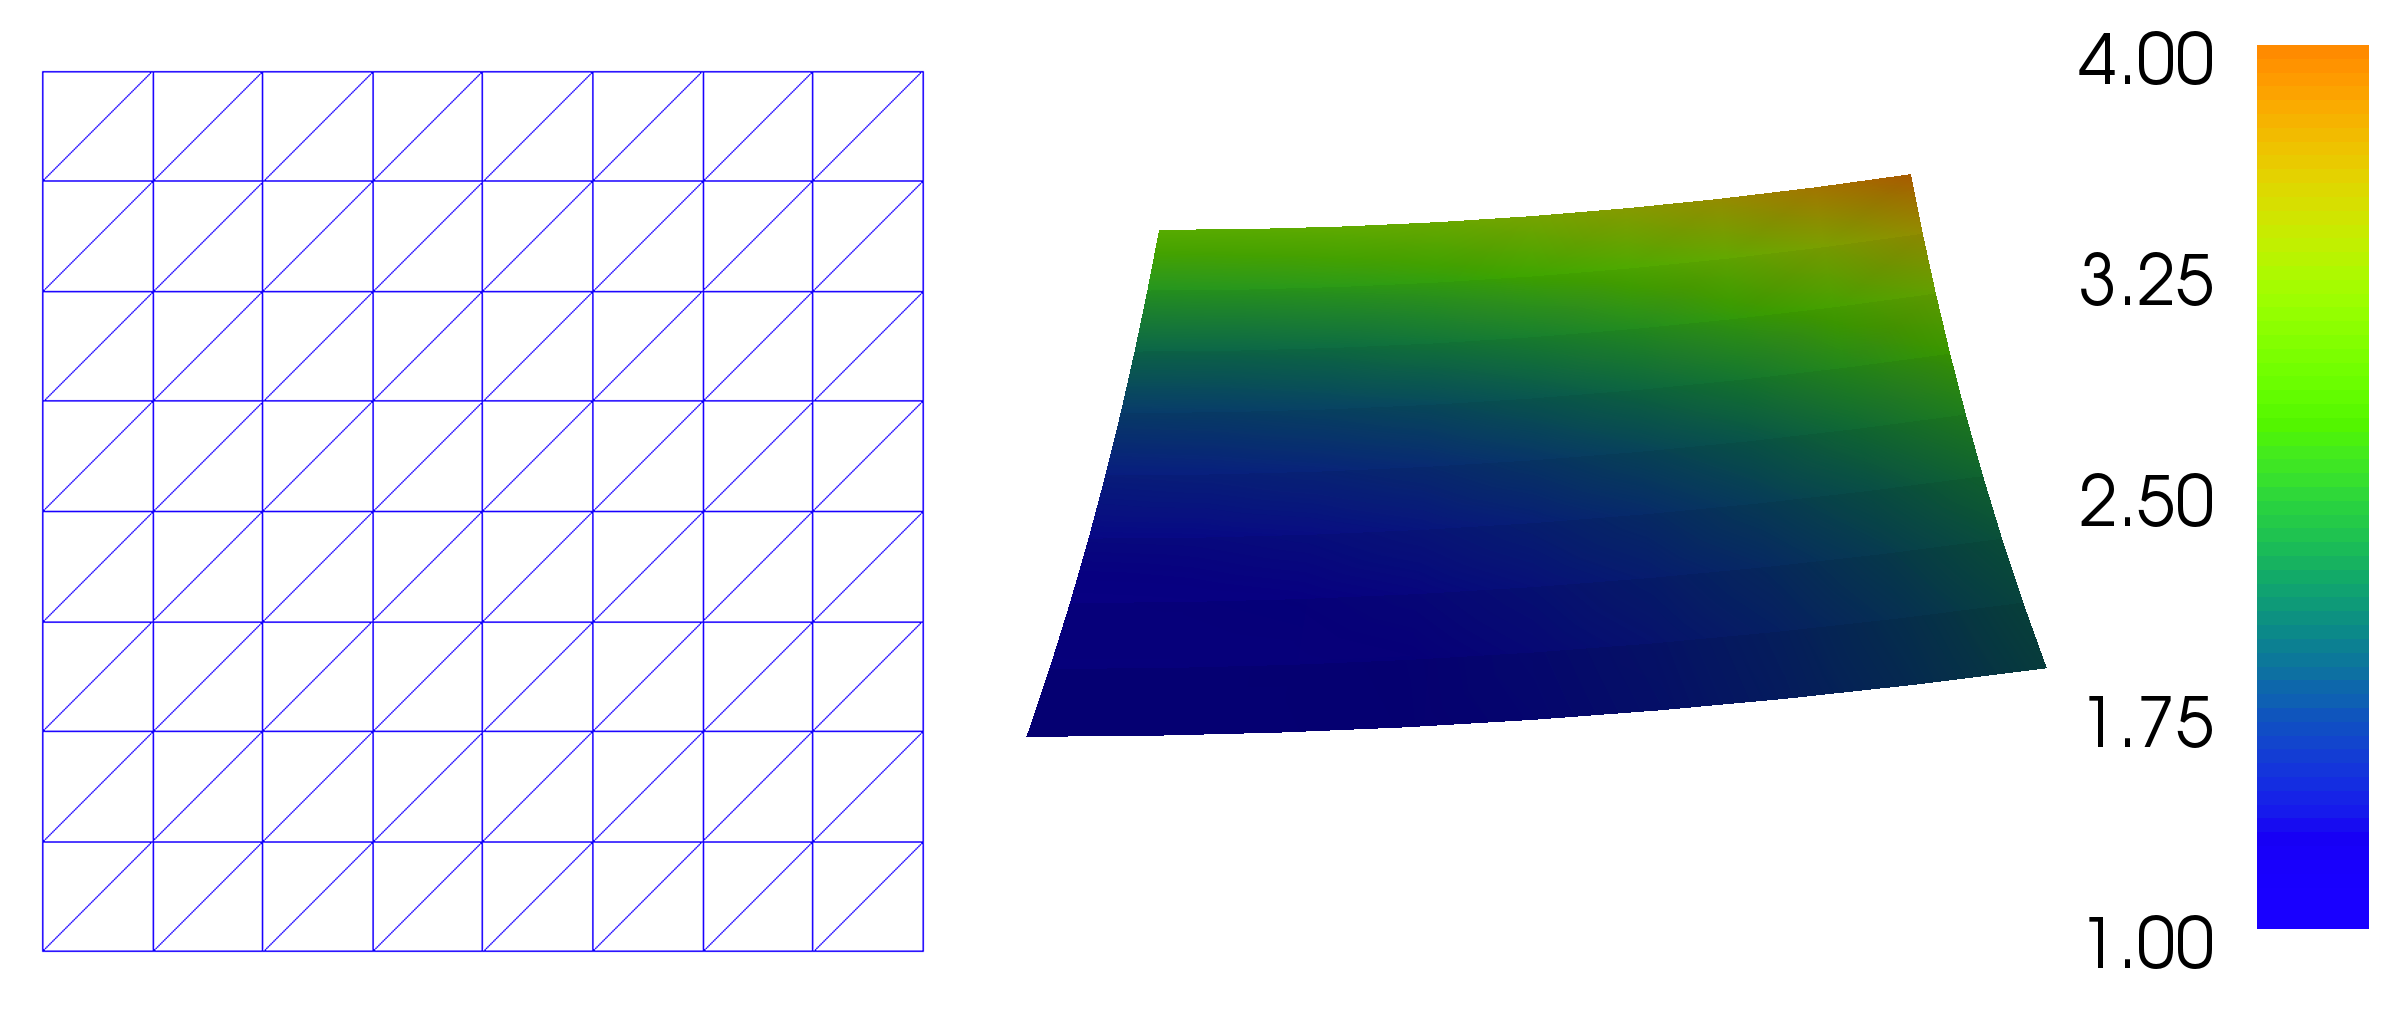
\includegraphics[width=0.95\linewidth]{fig/poisson_plot.png}}
  \caption{
  Plot of the mesh and the solution for the Poisson problem created using the built-in FEniCS visualization tool (\texttt{plot} command). \label{fig:poisson_plot}
  }
\end{figure}
%\clearpage % flush figures fig:poisson_plot

The \texttt{plot} command is useful for debugging and initial scientific
investigations. More advanced visualizations are better created by
exporting the solution to a file and using an advanced visualization
tool like ParaView, as explained in the next section.

By clicking the left mouse button in the plot window, you may rotate
the solution, while the right mouse button is used for zooming. Point
the mouse to the \texttt{Help} text in the lower left corner to display a
list of all available shortcut commands. The help menu may
alternatively be activated by typing \textbf{h} in the plot window. The
\texttt{plot} command also accepts a number of additional arguments, such as
for example setting the title of the plot window:

\begin{lstlisting}[language=Python,style=graycolor]
plot(u, title='Finite element solution')
plot(mesh, title='Finite element mesh')
\end{lstlisting}
For detailed documentation, either run the command \texttt{help(plot)} in
Python or \texttt{pydoc fenics.plot} from a terminal window.


\begin{warning_mdfboxadmon}[Built-in plotting on Mac OS X and in Docker]
The built-in plotting in FEniCS may not work as expected when either
running on Mac OS X or when running inside a FEniCS Docker container.
FEniCS supports plotting using the \texttt{plot} command on Mac OS
X. However, the keyboard shortcuts may fail
to work. When running inside a Docker container, plotting is not
supported since Docker does not interact with your windowing system.
For Docker users who need plotting, it is recommended to either work
within a Jupyter/FEniCS notebook (command \texttt{fenicsproject notebook})
or rely on ParaView or other external tools for visualization.
\end{warning_mdfboxadmon} % title: Built-in plotting on Mac OS X and in Docker

\subsection{Plotting the solution using ParaView}

\index{exporting solutions}
\index{postprocessing}
\index{ParaView}

The simple \texttt{plot} command is useful for quick visualizations, but for
more advanced visualizations an external tool must be used. In this
section we demonstrate how to visualize solutions in ParaView.
\href{{http://www.paraview.org}}{ParaView}\footnote{\texttt{http://www.paraview.org}} is a powerful
tool for visualizing scalar and vector fields, including those
computed by FEniCS.

The first step is to export the solution in VTK format:

\begin{lstlisting}[language=Python,style=graycolor]
vtkfile = File('poisson/solution.pvd')
vtkfile << u
\end{lstlisting}
The following steps demonstrate how to create a plot of the solution
of our Poisson problem in ParaView. The resulting plot is shown in
Figure~\ref{fig:poisson_paraview}.

\begin{enumerate}
\item Start the ParaView application.

\item Click \textbf{File--Open...} in the top menu and navigate to the directory containing the exported solution. This should be inside a subdirectory named \texttt{poisson} below the directory where the FEniCS Python program was started. Select the file named \texttt{solution.pvd} and then click \textbf{OK}.

\item Click \textbf{Apply} in the Properties pane on the left. This will bring up a plot of the solution.

\item To make a 3D plot of the solution, we will make use of one of ParaView's many \emph{filters}. Click \textbf{Filters--Alphabetical--Warp By Scalar} in the top menu and then \textbf{Apply} in the Properties pane on the left. This create an elevated surface with the height determined by the solution value.

\item To show the original plot below the elevated surface, click the little eye icon to the left of \texttt{solution.pvd} in the Pipeline Browser pane on the left. Also click the little 2D button at the top of the plot window to change the visualization to 3D. This lets you interact with the plot by rotating (left mouse button) and zooming (Ctrl + left mouse button).

\item To show the finite element mesh, click on \texttt{solution.pvd} in the Pipeline Browser, navigate to \textbf{Representation} in the Properties pane, and select \textbf{Surface With Edges}. This should make the finite element mesh visible.

\item To change the aspect ratio of the plot, click on \textbf{WarpByScalar1} in the Pipeline Browser and navigate to \textbf{Scale Factor} in the Properties pane. Change the value to 0.2 and click \textbf{Apply}. This will change the scale of the warped plot. We also unclick \textbf{Orientation Axis Visibility} at the bottom of the Properties pane to remove the little 3D axes in the lower left corner of the plot window. You should now see something that resembles the plot in Figure~\ref{fig:poisson_paraview}.

\item Finally, to export the visualization to a file, click \textbf{File--Save Screenshot...} and select a suitable file name such as \texttt{poisson.png}.
\end{enumerate}

\noindent
For more information, we refer to The ParaView Guide \cite{Paraview}
(free PDF available), the \href{{http://www.paraview.org/Wiki/The_ParaView_Tutorial}}{ParaView tutorial}\footnote{\texttt{http://www.paraview.org/Wiki/The\_ParaView\_Tutorial}}, and the instruction
video \href{{https://vimeo.com/34037236}}{Introduction to ParaView}\footnote{\texttt{https://vimeo.com/34037236}}.


\begin{figure}[!ht]  % fig:poisson_paraview
  \centerline{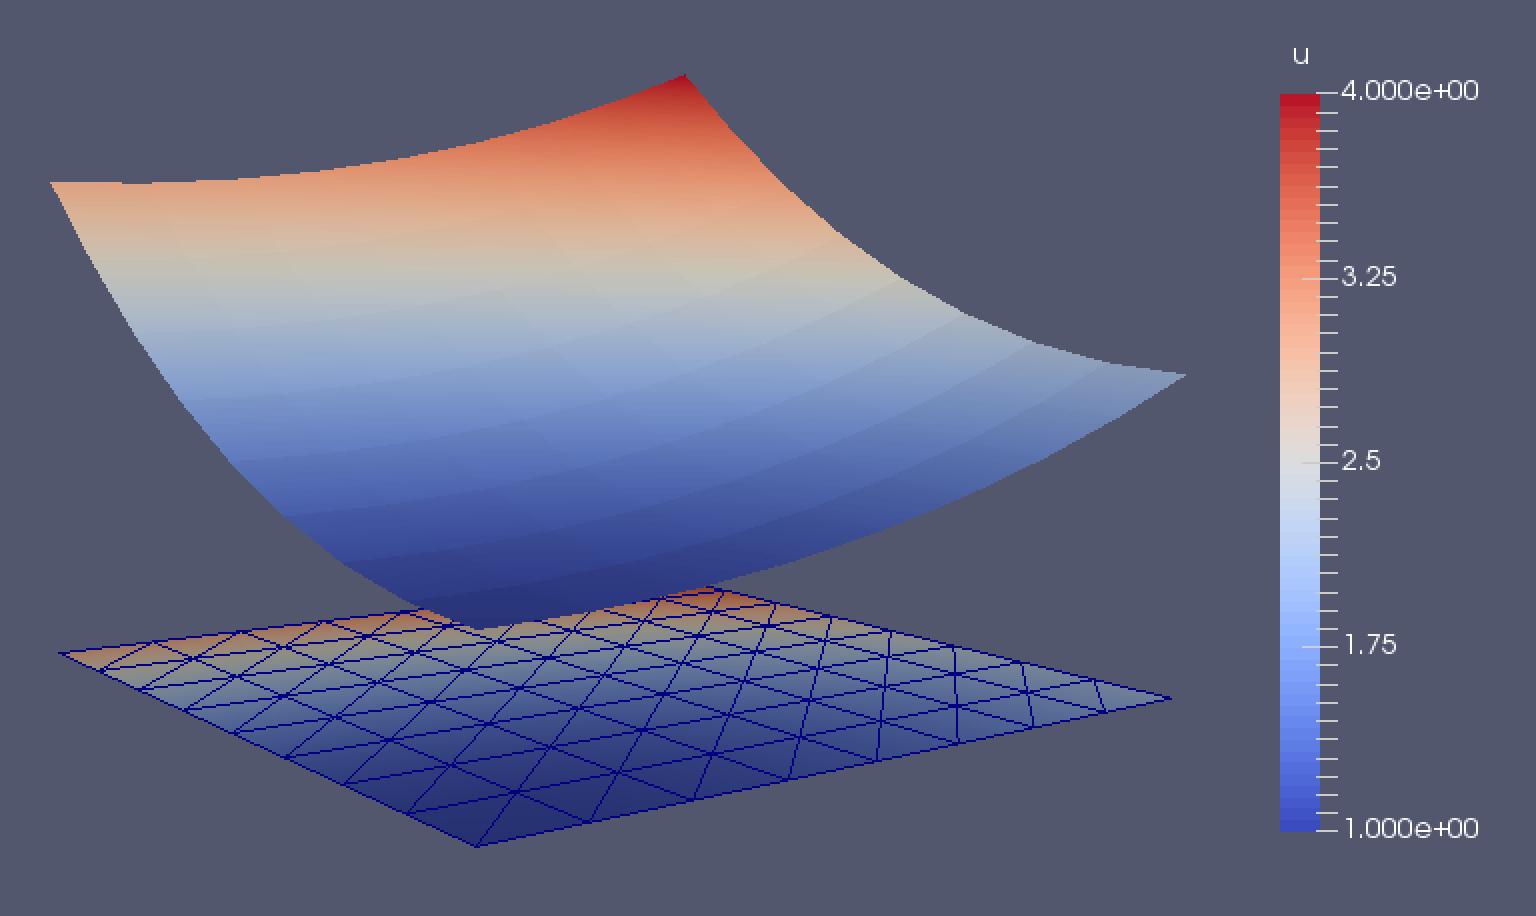
\includegraphics[width=0.95\linewidth]{fig/poisson_paraview.png}}
  \caption{
  Plot of the mesh and the solution for the Poisson problem created using ParaView. \label{fig:poisson_paraview}
  }
\end{figure}
%\clearpage % flush figures fig:poisson_paraview


\subsection{Computing the error}

\index{error}

Finally, we compute the error to check the accuracy of the solution.
We do this by comparing the finite element solution \texttt{u} with the exact
solution, which in this example happens to be the same as the
expression \Verb!u_D! used to set the boundary conditions. We compute the
error in two different ways. First, we compute the $L^2$ norm of the
error, defined by

\[ E = \sqrt{\int_\Omega (\ub - u)^2\dx}\tp\]
Since the exact solution is quadratic and the finite element solution
is piecewise linear, this error will be nonzero. To compute this error
in FEniCS, we simply write

\begin{lstlisting}[language=Python,style=graycolor]
error_L2 = errornorm(u_D, u, 'L2')
\end{lstlisting}
The \texttt{errornorm} function can also compute other error norms such
as the $H^1$ norm. Type \texttt{pydoc fenics.errornorm} in a terminal window
for details.

We also compute the maximum value of the error at all the vertices of
the finite element mesh. As mentioned above, we expect this error to
be zero to within machine precision for this particular example. To
compute the error at the vertices, we first ask FEniCS to compute the
value of both \Verb!u_D! and \texttt{u} at all vertices, and then subtract the
results:

\begin{lstlisting}[language=Python,style=graycolor]
vertex_values_u_D = u_D.compute_vertex_values(mesh)
vertex_values_u = u.compute_vertex_values(mesh)
import numpy as np
error_max = np.max(np.abs(vertex_values_u_D - vertex_values_u))
\end{lstlisting}
We have here used the maximum and absolute value functions from \texttt{numpy},
because these are much more efficient for large arrays (a factor of 30)
than Python's built-in \texttt{max} and \texttt{abs} functions.



\begin{notice_mdfboxadmon}[How to check that the error vanishes]
With inexact (floating point) arithmetic, the maximum
error at the vertices is not zero, but should be a small number. The
machine precision is about $10^{-16}$, but in finite element
calculations, rounding errors of this size may accumulate, to produce
an error larger than $10^{-16}$. Experiments show that increasing the
number of elements and increasing the degree of the finite element
polynomials increases the error. For a mesh with $2\times(20\times
20)$ cubic Lagrange elements (degree 3) the error is about $2\cdot
10^{-12}$, while for 128 linear elements the error is about $2\cdot
10^{-15}$.
\end{notice_mdfboxadmon} % title: How to check that the error vanishes

\subsection{Examining degrees of freedom and vertex values}
\label{ch:poisson0:impl:dofmap}

\index{degrees of freedom}
\index{vertex values}
\index{nodal values}
\index{dofs}

A finite element function like $u$ is expressed as a linear combination
of basis functions $\phi_j$, spanning the space $V$:

\begin{equation}
u = \sum_{j=1}^N U_j \phi_j \label{ch:poisson0:ufem}\tp
\end{equation}
By writing \texttt{solve(a == L, u, bc)} in the program, a linear system will
be formed from $a$ and $L$, and this system is solved for the
values $U_1,\ldots,U_N$. The values $U_1,\ldots,U_N$ are known as the
\emph{degrees of freedom} (``dofs'') or \emph{nodal values} of $u$. For Lagrange
elements (and many other element types) $U_j$ is simply the value of
$u$ at the node with global number $j$. The locations of the nodes and
cell vertices coincide for linear Lagrange elements, while for
higher-order elements there are additional nodes associated with the
facets, edges and sometimes also the interior of cells.

Having \texttt{u} represented as a \texttt{Function} object, we can either evaluate
\texttt{u(x)} at any point \texttt{x} in the mesh (expensive operation!), or we can
grab all the degrees of freedom in the vector $U$ directly by

\begin{lstlisting}[language=Python,style=graycolor]
nodal_values_u = u.vector()
\end{lstlisting}
The result is a \texttt{Vector} object, which is basically an encapsulation
of the vector object used in the linear algebra package that is used
to solve the linear system arising from the variational problem.
Since we program in Python it is convenient to convert the \texttt{Vector}
object to a standard \texttt{numpy} array for further processing:

\index{degrees of freedom}
\index{nodal values}
\index{numbering!degrees of freedom}
\index{numbering!cell vertices}

\begin{lstlisting}[language=Python,style=graycolor]
array_u = nodal_values_u.array()
\end{lstlisting}

With \texttt{numpy} arrays we can write MATLAB-like code to analyze the
data. Indexing is done with square brackets: \Verb!array_u[j]!, where the
index \texttt{j} always starts at \texttt{0}. If the solution is computed with
piecewise linear Lagrange elements ($\mathsf{P}_1$), then the size of
the array \Verb!array_u! is equal to the number of vertices, and each
\Verb!array_u[j]! is the value at some vertex in the mesh. However, the degrees
of freedom are not necessarily numbered in the same way as the
vertices of the
mesh. (This is discussed in some detail in Section~\ref{ch:poisson0:verify1}).
If we therefore want to know the values at the vertices, we need to
call the function \Verb!u.compute_vertex_values!. This function returns
the values at all the vertices of the mesh as a \texttt{numpy} array with the same
numbering as for the vertices of the mesh, for example:

\begin{lstlisting}[language=Python,style=graycolor]
vertex_values_u = u.compute_vertex_values()
\end{lstlisting}
Note that for $\mathsf{P}_1$ elements, the arrays \Verb!array_u! and \Verb!vertex_values_u! have the same lengths and contain the same values, albeit in different order.


% !split
% Stand-alone notebook?

\section{Deflection of a membrane}
\label{ch:poisson0:membrane}

Our first FEniCS program for the Poisson equation targeted a
simple test problem where we could easily verify the
implementation. We now turn our attention to a physically more
relevant problem with solutions of somewhat more exciting shape.

We want to compute the deflection $D(x,y)$ of a two-dimensional,
circular membrane of radius $R$, subject to a load $p$ over the
membrane. The appropriate PDE model is

\begin{equation}
-T\nabla^2 D = p\quad\hbox{in }\Omega = \{ (x,y)\,\vert\, x^2+y^2\leq R\}\tp
\end{equation}
Here, $T$ is the tension in the membrane (constant), and $p$ is the external
pressure load.
The boundary of the membrane has no
deflection, implying $D=0$ as a boundary condition.
A localized load can be modeled as a Gaussian function:

\begin{equation}
p(x,y) = {A\over 2\pi\sigma}\exp{\left(
- {1\over2}\left( {x-x_0\over\sigma}\right)^2
- {1\over2}\left( {y-y_0\over\sigma}\right)^2
\right)}\, .
\end{equation}
The parameter $A$ is the amplitude of the pressure, $(x_0,y_0)$ the
localization of the maximum point of the load, and $\sigma$ the
``width'' of $p$. We will take the center $(x_0,y_0)$ of the pressure
to be $(0, R_0)$ for some $0 < R_0 < R$.

\subsection{Scaling the equation}

There are many physical parameters in this problem, and we can benefit
from grouping them by means of scaling. Let us introduce dimensionless
coordinates $\bar x = x/R$, $\bar y = y/R$, and a dimensionless
deflection $w=D/D_c$, where $D_c$ is a characteristic size of the
deflection. Introducing $\bar R_0=R_0/R$, we obtain

\[ -\frac{\partial^2 w}{\partial\bar x^2}
-\frac{\partial^2 w}{\partial\bar y^2}= \alpha
\exp{\left(
- \beta^2(\bar x^2
+ (\bar y-\bar R_0)^2)\right)}\hbox{ for } \bar x^2 + \bar y^2 < 1,\]
where

\[ \alpha = \frac{R^2A}{2\pi T D_c\sigma},\quad\beta = \frac{R}{\sqrt{2}\sigma}\tp\]
With an appropriate scaling, $w$ and its derivatives are of size
unity, so the left-hand side of the scaled PDE is about unity in size,
while the right-hand side has $\alpha$ as its characteristic size.
This suggest choosing $\alpha$ to be unity, or around unity. We shall
in this particular case choose $\alpha=4$. (One can also find the
analytical solution in scaled coordinates and show that the maximum
deflection $D(0,0)$ is $D_c$ if we choose $\alpha=4$ to determine
$D_c$.) With $D_c=AR^2/(8\pi\sigma T)$ and dropping the bars we obtain
the scaled problem

\begin{equation}
-\nabla^2w = 4\exp{\left(
- \beta^2(x^2
+ (y-R_0)^2)\right)},
\label{ch:poisson0:membrane:scaled:eq}
\end{equation}
to be solved over the unit disc with $w=0$ on the boundary. Now
there are only two parameters to vary: the dimensionless extent of the
pressure, $\beta$, and the localization of the pressure peak, $R_0\in
[0,1]$.  As $\beta\rightarrow 0$, the solution will approach the
special case $w=1-x^2-y^2$.

Given a computed scaled solution $w$, the physical deflection can be computed by

\[ D = \frac{AR^2}{8\pi\sigma T}w\tp\]

Just a few modifications are necessary to our previous program to solve
this new problem.

\subsection{Defining the mesh}

A mesh over the unit disk can be created by the \texttt{mshr} tool in
FEniCS:

\begin{lstlisting}[language=Python,style=graycolor]
from mshr import *
domain = Circle(Point(0, 0), 1)
mesh = generate_mesh(domain, 64)
\end{lstlisting}
The \texttt{Circle} shape from \texttt{mshr} takes the center and radius of the
circle as arguments. The second argument to the \Verb!generate_mesh!
function specifies the desired mesh resolution. The cell size will be
(approximately) equal to the diameter of the domain divided by the
resolution.

\subsection{Defining the load}

\index{Expression@{\rm\texttt{Expression}}}

The right-hand side pressure function
is represented by an \texttt{Expression} object. There
are two physical parameters in the formula for $f$ that enter the
expression string and these parameters must have their values set
by keyword arguments:

\begin{lstlisting}[language=Python,style=graycolor]
beta = 8
R0 = 0.6
p = Expression('4*exp(-pow(beta, 2)*(pow(x[0], 2) + pow(x[1] - R0, 2)))',
               degree=1, beta=beta, R0=R0)
\end{lstlisting}
The coordinates in \texttt{Expression} objects are always an array
\texttt{x} with components \texttt{x[0]}, \texttt{x[1]}, and \texttt{x[2]}, corresponding to
$x$, $y$, and $z$.
Otherwise we are free to introduce names of parameters as long as
these are given default values by keyword arguments. All the
parameters initialized by keyword arguments can at any time have their
values modified. For example, we may set

\begin{lstlisting}[language=Python,style=graycolor]
p.beta = 12
p.R0 = 0.3
\end{lstlisting}

\subsection{Defining the variational problem}

The variational problem and the boundary conditions are the same as in
our first Poisson problem, but we may introduce \texttt{w} instead of \texttt{u} as
primary unknown and \texttt{p} instead of \texttt{f} as right-hand side function:

\begin{lstlisting}[language=Python,style=graycolor]
w = TrialFunction(V)
v = TestFunction(V)
a = dot(grad(w), grad(v))*dx
L = p*v*dx

w = Function(V)
solve(a == L, w, bc)
\end{lstlisting}

% Avoid plot command in notebook. It easily makes the kernel freeze.

\subsection{Plotting the solution}

It is of interest to visualize the pressure $p$ along with the
deflection $w$ so that we may examine the membrane's response to the
pressure. We must then transform the formula (\texttt{Expression}) to a
finite element function (\texttt{Function}). The most natural approach is to
construct a finite element function whose degrees of freedom are
calculated from $p$. That is, we interpolate $p$ to the function space
$V$:

\begin{lstlisting}[language=Python,style=graycolor]
p = interpolate(p, V)
\end{lstlisting}
Note that the assignment to \texttt{p} destroys the previous \texttt{Expression}
object \texttt{p}, so if it is of interest to still have access to this
object, another name must be used for the \texttt{Function} object returned
by \texttt{interpolate}. The two functions \texttt{w} and \texttt{p} may be plotted
using the built-in plot command:

\begin{lstlisting}[language=Python,style=graycolor]
plot(w, title='Deflection')
plot(p, title='Load')
\end{lstlisting}
As before, we also export the solutions in VTK format for
visualization in ParaView:

\begin{lstlisting}[language=Python,style=graycolor]
vtkfile_w = File('poisson_membrane/deflection.pvd')
vtkfile_w << w
vtkfile_p = File('poisson_membrane/load.pvd')
vtkfile_p << p
\end{lstlisting}
Figure~\ref{fig:poisson_membrane_deflection_load} shows a visualization
of the deflection \texttt{w} and the load \texttt{p} created with ParaView.


\begin{figure}[!ht]  % fig:poisson_membrane_deflection_load
  \centerline{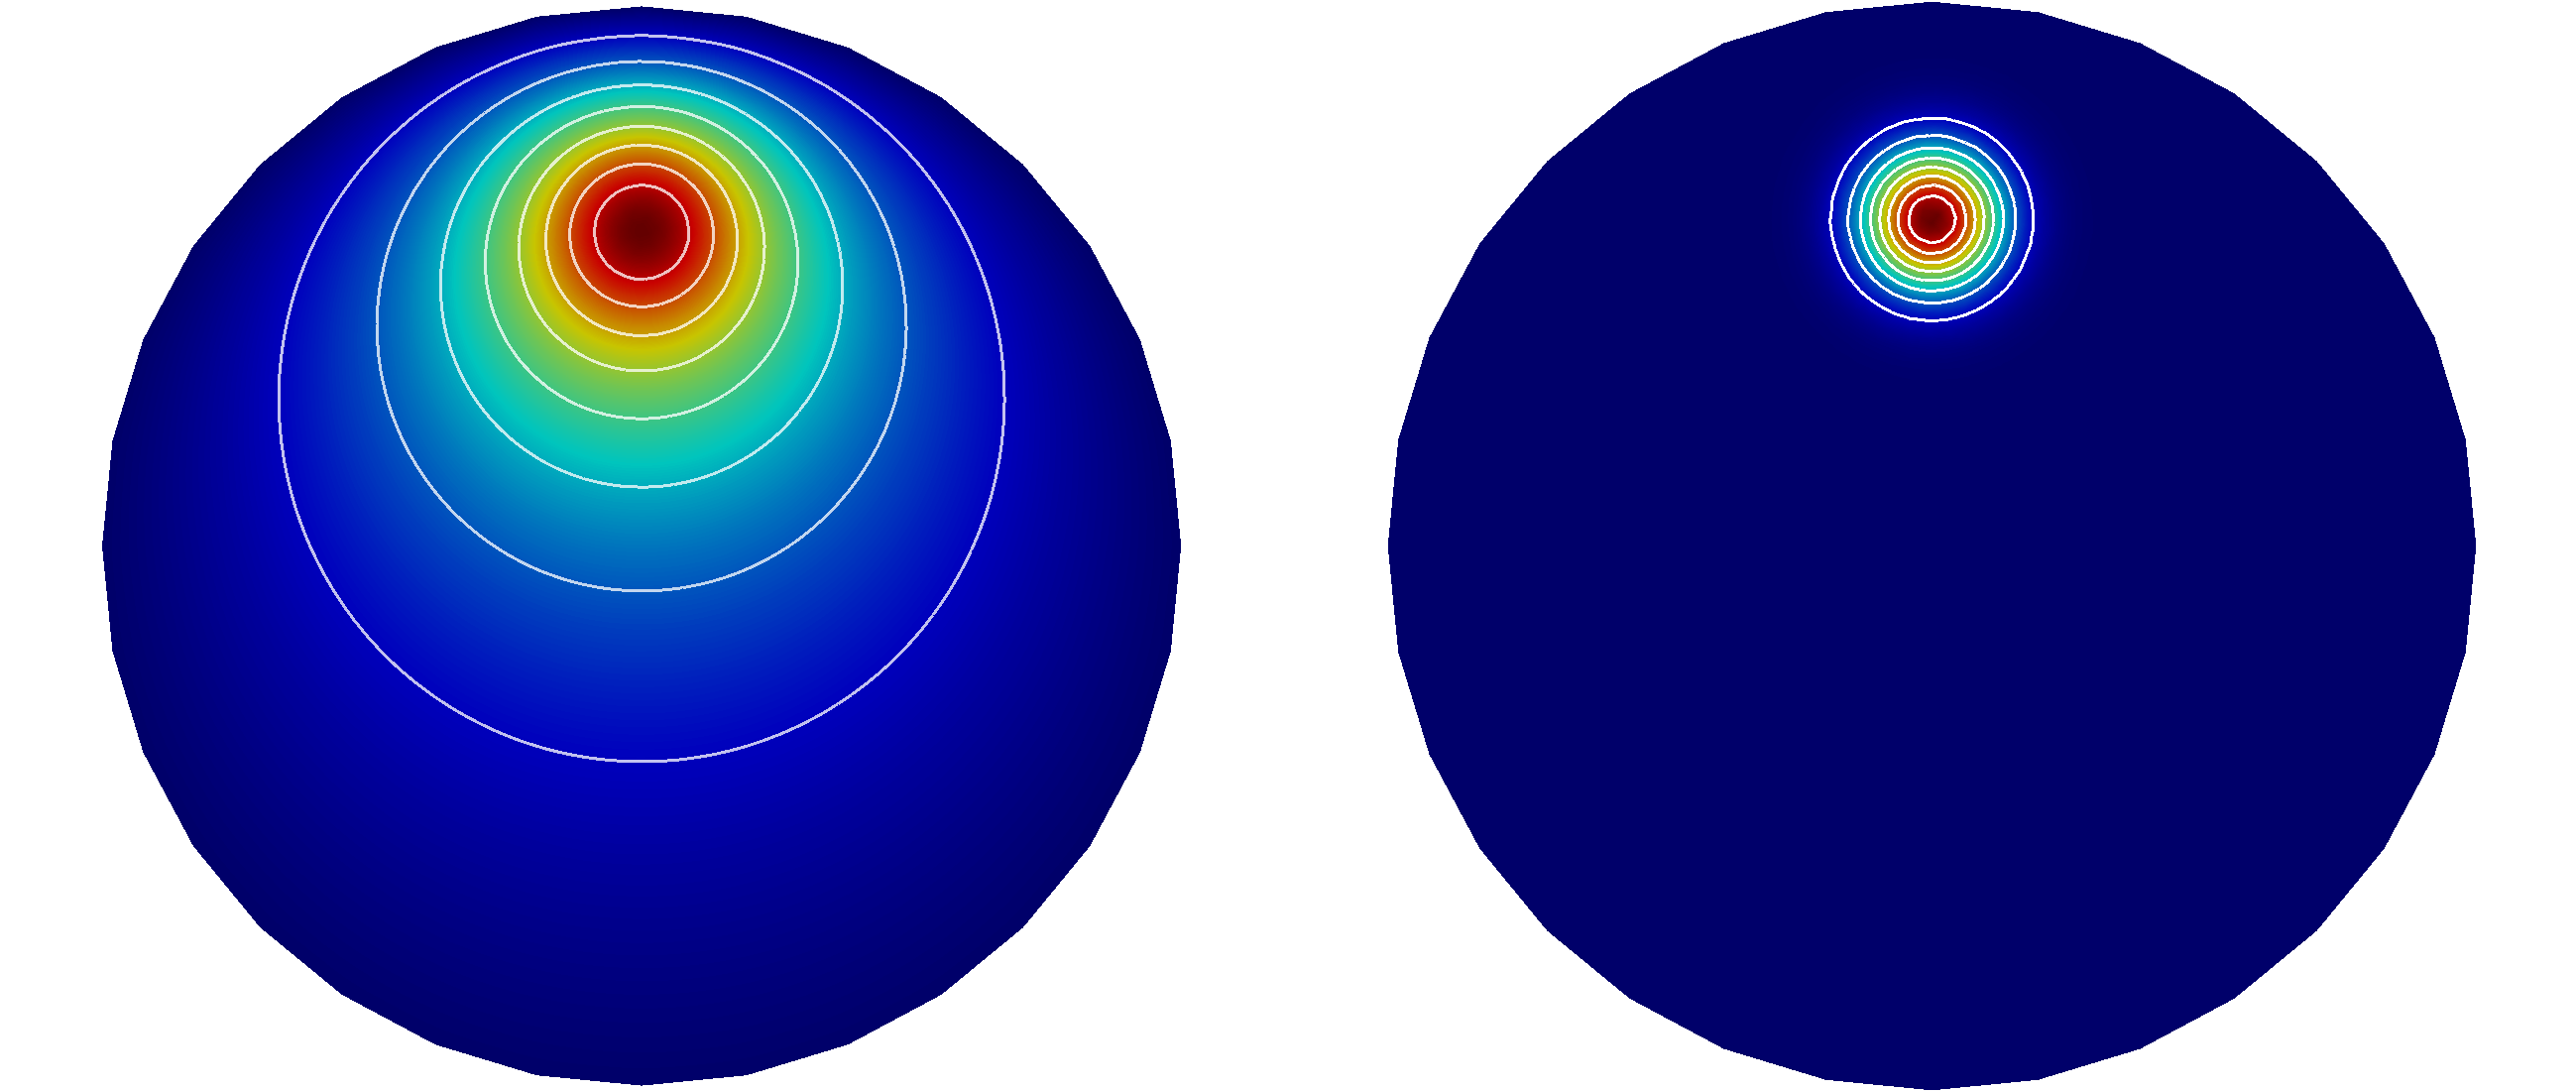
\includegraphics[width=0.95\linewidth]{fig/poisson_membrane_deflection_load.png}}
  \caption{
  Plot of the deflection (left) and load (right) for the membrane problem created using ParaView. The plot uses 10 equispaced isolines for the solution values and the optional \emph{jet} colormap. \label{fig:poisson_membrane_deflection_load}
  }
\end{figure}
%\clearpage % flush figures fig:poisson_membrane_deflection_load

\subsection{Making curve plots through the domain}

\index{curve plots}

% Nice with some matplotlib plots in notebooks...and very useful for
% scientific investigations.

Another way to compare the deflection and the load is to make a curve plot
along the line $x=0$. This is just a matter of defining a set of points
along the $y$-axis and evaluating the finite element functions \texttt{w} and \texttt{p}
at these points:

\begin{lstlisting}[language=Python,style=graycolor]
# Curve plot along x = 0 comparing p and w
import numpy as np
import matplotlib.pyplot as plt
tol = 0.001  # avoid hitting points outside the domain
y = np.linspace(-1 + tol, 1 - tol, 101)
points = [(0, y_) for y_ in y]  # 2D points
w_line = np.array([w(point) for point in points])
p_line = np.array([p(point) for point in points])
plt.plot(y, 50*w_line, 'k', linewidth=2)  # magnify w
plt.plot(y, p_line, 'b--', linewidth=2)
plt.grid(True)
plt.xlabel('$y$')
plt.legend(['Deflection ($\\times 50$)', 'Load'], loc='upper left')
plt.savefig('poisson_membrane/curves.pdf')
plt.savefig('poisson_membrane/curves.png')
\end{lstlisting}
This example program can be found in the file \href{{https://fenicsproject.org/pub/tutorial/python/vol1/ft02_poisson_membrane.py}}{\nolinkurl{ft02_poisson_membrane.py}}.

\index{ft02\_poisson\_membrane.py@{\rm\texttt{ft02\_poisson\_membrane.py}}}
The resulting curve plot is shown in Figure~\ref{fig:poisson_membrane_curves}. The localized input ($p$) is heavily
damped and smoothed in the output ($w$). This reflects a typical
property of the Poisson equation.


\begin{figure}[!ht]  % fig:poisson_membrane_curves
  \centerline{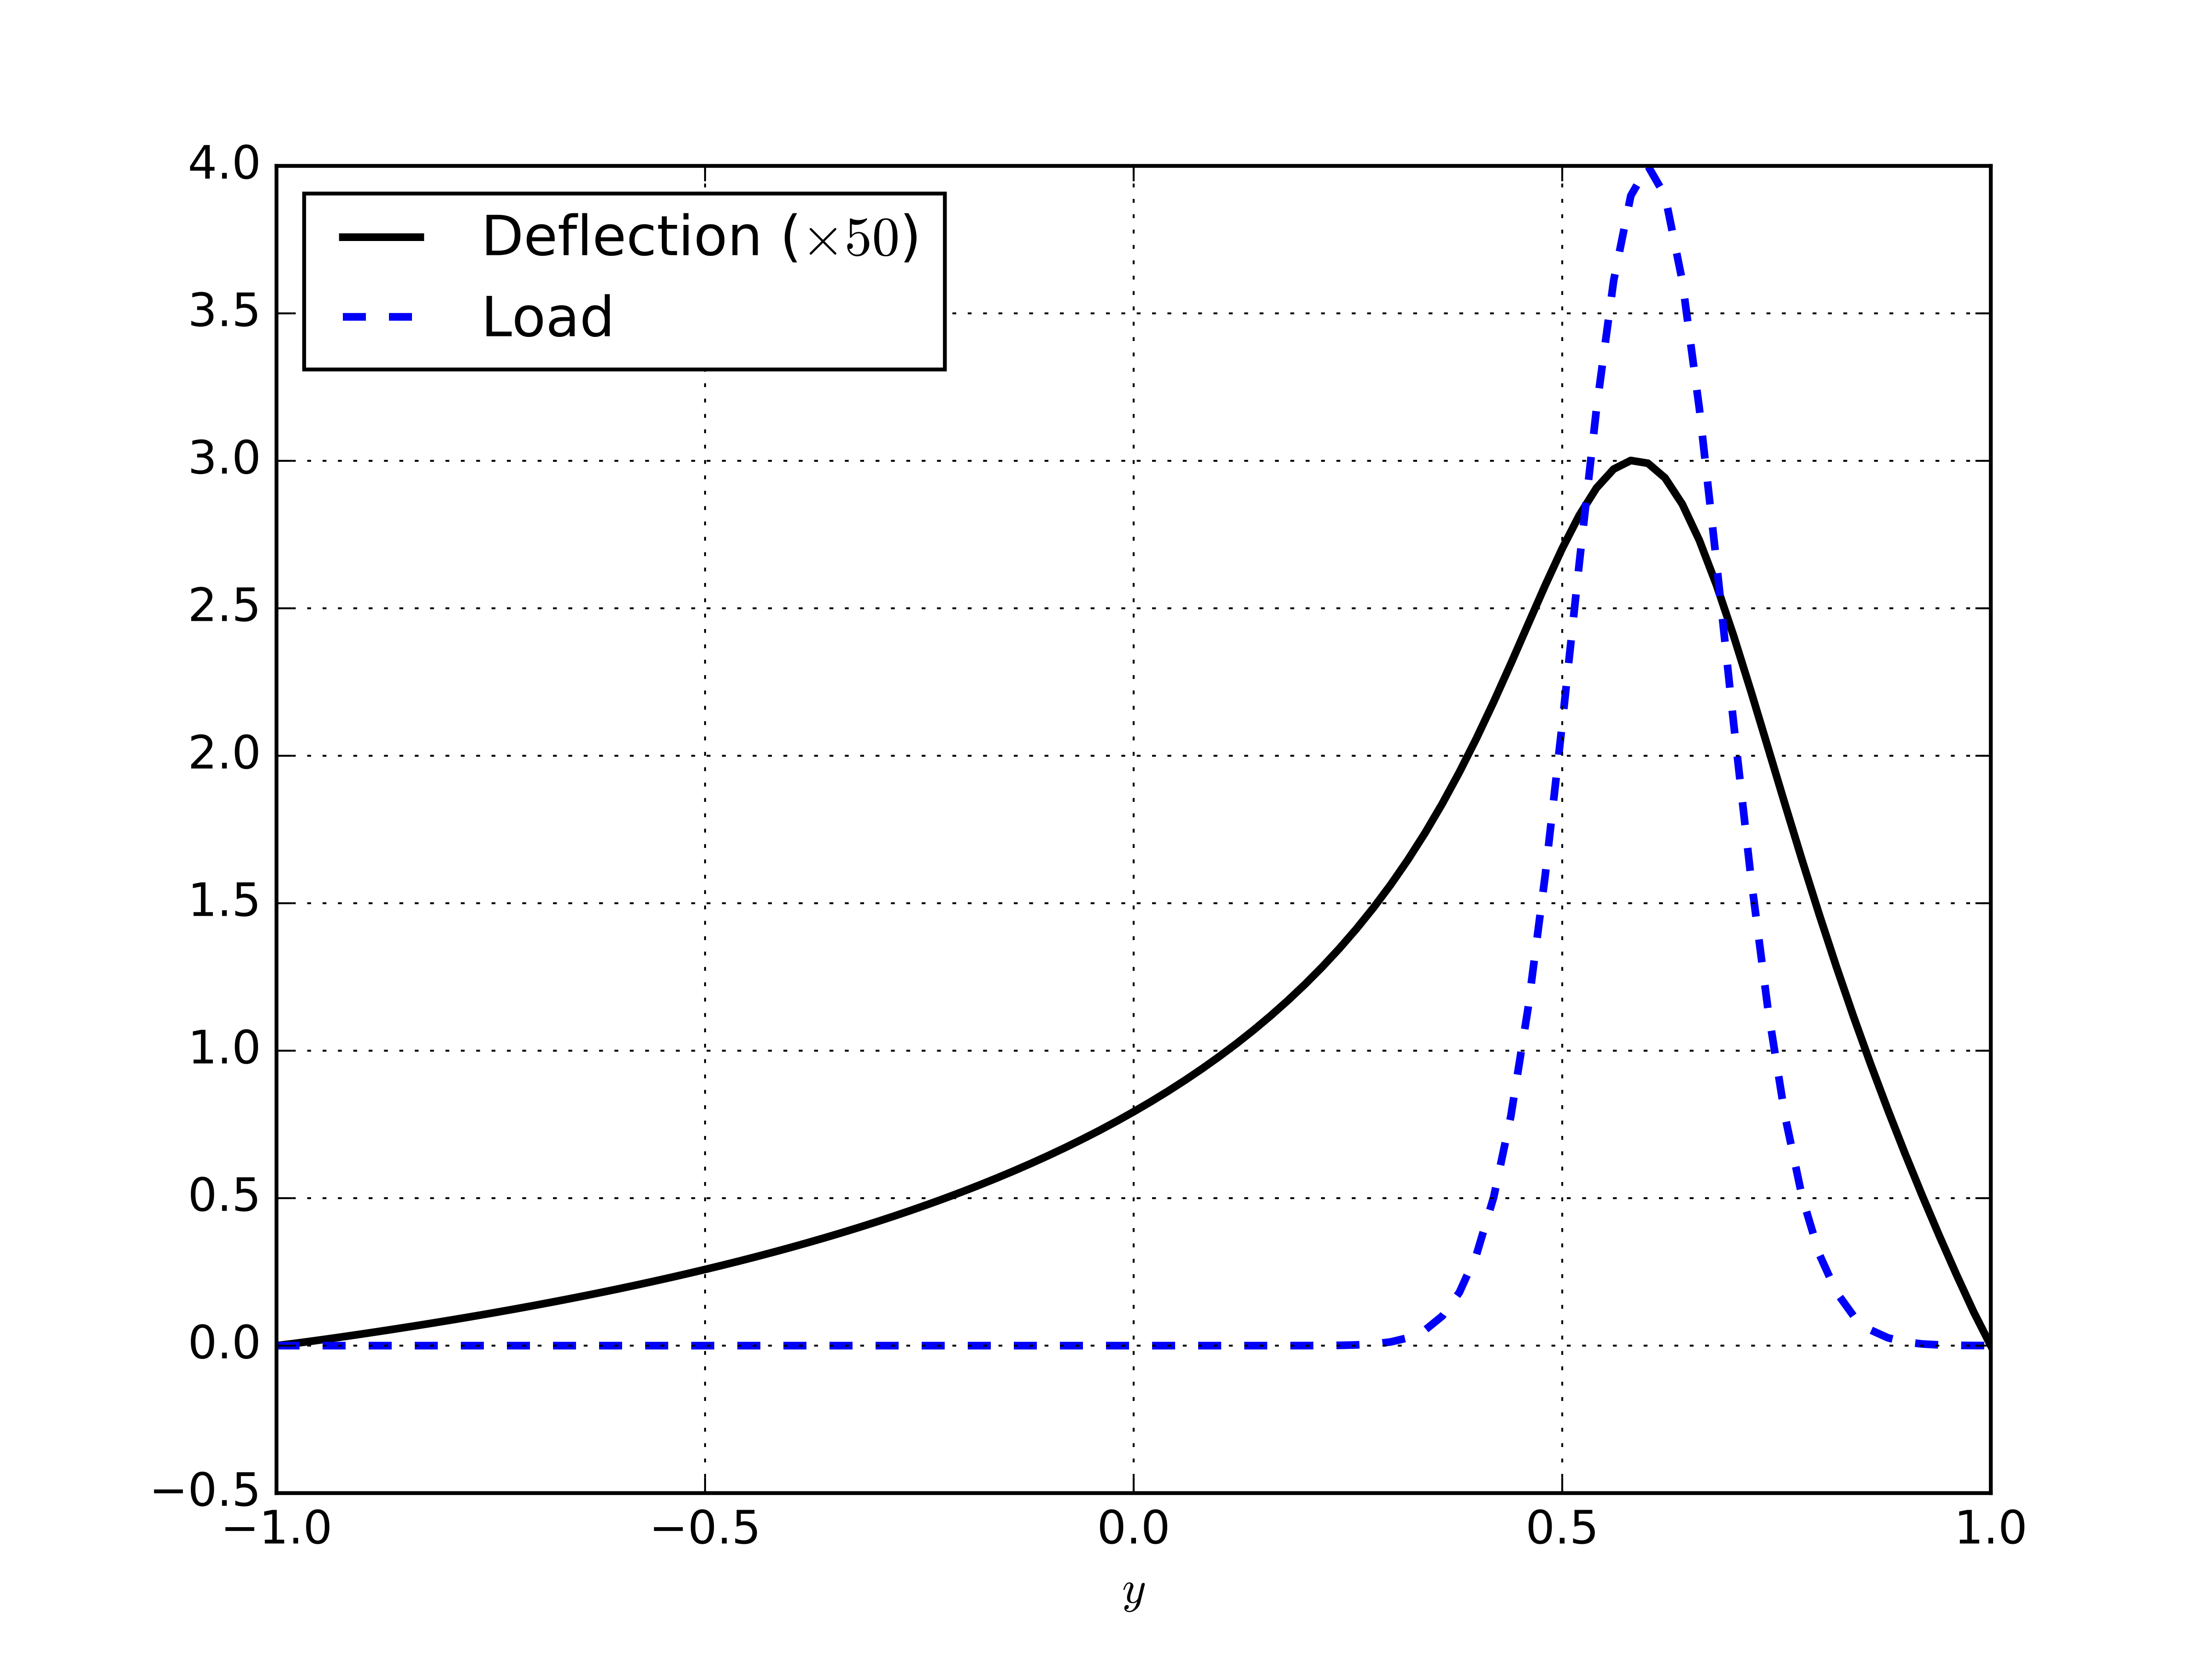
\includegraphics[width=0.95\linewidth]{fig/poisson_membrane_curves.png}}
  \caption{
  Plot of the deflection and load for the membrane problem created using Matplotlib and sampling of the two functions along the $y$-axsis. \label{fig:poisson_membrane_curves}
  }
\end{figure}
%\clearpage % flush figures fig:poisson_membrane_curves

% !split
\chapter{A Gallery of finite element solvers}
\label{ch:gallery}


\begin{quote}
The goal of this chapter is to demonstrate how a range of important
PDEs from science and engineering can be quickly solved with a few
lines of FEniCS code. We start with the heat equation and continue
with a nonlinear Poisson equation, the equations for linear
elasticity, the Navier--Stokes equations, and finally look at how to
solve systems of nonlinear advection--diffusion--reaction
equations. These problems illustrate how to solve time-dependent
problems, nonlinear problems, vector-valued problems, and systems of
PDEs. For each problem, we derive the variational formulation and
express the problem in Python in a way that closely resembles the
mathematics.
\end{quote}


% Stand-alone notebook?

\section{The heat equation}
\label{ch:fundamentals:diffusion}

\index{heat equation}
\index{time-dependent problem}

As a first extension of the Poisson problem from the previous chapter,
we consider the time-dependent heat equation, or the time-dependent
diffusion equation. This is the natural extension of the Poisson
equation describing the stationary distribution of heat in a body to a
time-dependent problem.

We will see that by discretizing time into small time intervals and
applying standard time-stepping methods, we can solve the heat
equation by solving a sequence of variational problems, much like the
one we encountered for the Poisson equation.

\subsection{PDE problem}

Our model problem for time-dependent PDEs reads

\begin{alignat}{2}
{\partial u\over\partial t} &= \nabla^2 u + f \quad &&\hbox{in }\Omega\times(0, T],
\label{ch:diffusion0:pde1}\\
u &= \ub &&\hbox{on } \partial \Omega\times(0, T],
\label{ch:diffusion0:pde1:bc}\\
u &= \uI &&\mbox{at } t=0\tp
\label{ch:diffusion0:pde1:ic}
\end{alignat}
Here, $u$ varies with space and time, e.g., $u=u(x,y,t)$ if the spatial
domain $\Omega$ is two-dimensional. The source function $f$ and the
boundary values $\ub$ may also vary with space and time.
The initial condition $\uI$ is a function of space only.

\subsection{Variational formulation}
\label{ftut:timedep:diffusion1}

A straightforward approach to solving time-dependent PDEs by the
finite element method is to first discretize the time derivative by a
finite difference approximation, which yields a sequence of
stationary problems, and then turn each stationary problem into a
variational formulation.

Let superscript $n$ denote a quantity at time $t_n$, where $n$ is an
integer counting time levels. For example, $u^n$ means $u$ at time
level $n$. A finite difference discretization in time first consists
of sampling the PDE at some time level, say $t_{n+1}$:

\index{time step}

\begin{equation}
\left({\partial u \over\partial t}\right)^{n+1} = \nabla^2 u^{n+1} + f^{n+1}\tp
\label{ch:diffusion0:pde1:tk}
\end{equation}
The time-derivative can be approximated by a difference quotient.
For simplicity and stability reasons, we choose a
simple backward difference:

\index{implicit Euler}
\index{backward difference}

\begin{equation}
\left({\partial u\over\partial t}\right)^{n+1}\approx {{u^{n+1} - u^n}\over{\dt}},
\label{ch:diffusion0:BE}
\end{equation}
where $\dt$ is the time discretization parameter.
Inserting (\ref{ch:diffusion0:BE}) in (\ref{ch:diffusion0:pde1:tk}) yields

\begin{equation}
{{u^{n+1} - u^n}\over{\dt}} = \nabla^2 u^{n+1} + f^{n+1}\tp
\label{ch:diffusion0:pde1:BE}
\end{equation}
This is our time-discrete version of the heat equation
(\ref{ch:diffusion0:pde1}), a so-called \emph{backward Euler} or \emph{implicit
Euler} discretization.

We may reorder (\ref{ch:diffusion0:pde1:BE}) so
that the left-hand side contains the terms with the unknown $u^{n+1}$ and
the right-hand side contains computed terms only. The result
is a sequence of spatial (stationary) problems for $u^{n+1}$, assuming
$u^n$ is known from the previous time step:

\begin{align}
u^0 &= \uI, \label{ch:diffusion0:pde1:u0}\\
u^{n+1} - {\dt}\nabla^2 u^{n+1} &=  u^n + {\dt} f^{n+1},\quad n=0,1,2,\ldots
\label{ch:diffusion0:pde1:uk}
\end{align}
Given $\uI$, we can solve for $u^0$, $u^1$, $u^2$, and so on.

An alternative to (\ref{ch:diffusion0:pde1:uk}), which can be
convenient in implementations, is to collect
all terms on one side of the equality sign:

\begin{equation}
u^{n+1} - {\dt}\nabla^2 u^{n+1} -  u^{n} - {\dt} f^{n+1} = 0,\quad n=0,1,2,\ldots
\label{ch:diffusion0:pde1:uk2}
\end{equation}

We use a finite element method to solve
(\ref{ch:diffusion0:pde1:u0}) and either of the equations
(\ref{ch:diffusion0:pde1:uk}) or (\ref{ch:diffusion0:pde1:uk2}).  This
requires turning the equations into weak forms.  As usual, we multiply
by a test function $v\in \hat V$ and integrate second-derivatives by
parts. Introducing the symbol $u$ for $u^{n+1}$ (which is natural in the
program), the resulting weak form arising from
formulation (\ref{ch:diffusion0:pde1:uk})
can be conveniently written in
the standard notation:

\[ a(u,v)=L_{n+1}(v),\]
where

\begin{align}
a(u,v) &= \int_\Omega\left(uv + {\dt}
\nabla u\cdot \nabla v\right) \dx, \label{ch:diffusion0:pde1:a}\\
L_{n+1}(v) &= \int_\Omega \left(u^n + {\dt}  f^{n+1}\right)v \dx\tp
\label{ch:diffusion0:pde1:L}
\end{align}
The alternative form (\ref{ch:diffusion0:pde1:uk2}) has an
abstract formulation

\[ F_{n+1}(u;v) = 0,\]
where

\begin{equation}
F_{n+1}(u; v) = \int_\Omega \left(uv + {\dt}
\nabla u\cdot \nabla v -
(u^n + {\dt} f^{n+1})v\right) \dx\tp
\label{ch:diffusion0:pde1:F}
\end{equation}

In addition to the variational problem to be solved in each time step,
we also need to approximate the initial condition
(\ref{ch:diffusion0:pde1:u0}). This equation can also be turned into a
variational problem:

\[ a_0(u,v)=L_0(v),\]
with

\begin{align}
a_0(u,v) &= \int_\Omega uv \dx, \label{ch:diffusion0:pde1:a0}\\
L_0(v) &= \int_\Omega \uI v \dx\tp \label{ch:diffusion0:pde1:L0}
\end{align}
When solving this variational problem, $u^0$ becomes the $L^2$
projection of the given initial value $\uI$ into the finite element
space. The alternative is to construct $u^0$ by just interpolating the
initial value $\uI$; that is, if $u^0=\sum_{j=1}^N U^0_j\phi_j$, we
simply set $U_j=\uI(x_j,y_j)$, where $(x_j,y_j)$ are the coordinates
of node number $j$. We refer to these two strategies as computing the
initial condition by either projection or interpolation. Both
operations are easy to compute in FEniCS through a single statement,
using either the \texttt{project} or \texttt{interpolate} function. The most common
choice is \texttt{project}, which computes an approximation to $\uI$, but in
some applications where we want to verify the code by reproducing
exact solutions, one must use \texttt{interpolate} (and we use such a test
problem here!).

\index{interpolate@{\rm\texttt{interpolate}}}
\index{project@{\rm\texttt{project}}}

In summary, we thus need to solve the following sequence of variational
problems to compute the finite element solution to the heat equation:
find $u^0\in V$ such that $a_0(u^0,v)=L_0(v)$ holds for all $v\in\hat V$,
and then find $u^{n+1}\in V$
such that $a(u^{n+1},v)=L_{n+1}(v)$ for all $v\in\hat V$,
or alternatively, $F_{n+1}(u^{n+1},v)=0$ for all $v\in\hat V$,
for $n=0,1,2,\ldots$.

\subsection{FEniCS implementation}
\label{ftut:timedep:diffusion1:impl}

Our program needs to implement the time-stepping manually, but can
rely on FEniCS to easily compute $a_0$, $L_0$, $a$, and $L$ (or
$F_{n+1}$), and solve the linear systems for the unknowns.

\paragraph{Test problem 1: A known analytical solution.}
Just as for the Poisson problem from the previous chapter, we
construct a test problem that makes it easy to determine if the
calculations are correct. Since we know that our first-order
time-stepping scheme is exact for linear functions, we create a test
problem which has a linear variation in time. We combine this with a
quadratic variation in space. We thus take

\begin{equation} u = 1 + x^2 + \alpha y^2 + \beta t,
\label{ch:diffusion0:pde1:u0test}
\end{equation}
which yields a function whose computed values at the nodes will be
exact, regardless of the size of the elements and $\dt$, as long as
the mesh is uniformly partitioned. By inserting
(\ref{ch:diffusion0:pde1:u0test}) into the heat equation
(\ref{ch:diffusion0:pde1}), we find that the right-hand side $f$ must
be given by $f(x,y,t)=\beta - 2 - 2\alpha$. The boundary value
is $\ub(x, y, t) = 1 + x^2 + \alpha y^2 + \beta t$ and the initial
value is $\uI(x, y) = 1 + x^2 + \alpha y^2$.

\paragraph{FEniCS implementation.}
A new programming issue is how to deal with functions that vary in
space \emph{and time}, such as the boundary condition $\ub(x, y,
t) = 1 + x^2 + \alpha y^2 + \beta t$. A natural solution is to use a
FEniCS \texttt{Expression} with time $t$ as a parameter, in addition to the
parameters $\alpha$ and $\beta$:

\index{time-dependent expression}

\begin{lstlisting}[language=Python,style=graycolor]
alpha = 3; beta = 1.2
u_D = Expression('1 + x[0]*x[0] + alpha*x[1]*x[1] + beta*t',
                 degree=2, alpha=alpha, beta=beta, t=0)
\end{lstlisting}
This \texttt{Expression} uses the components of \texttt{x} as independent
variables, while \texttt{alpha}, \texttt{beta}, and \texttt{t} are parameters. The
time \texttt{t} can later be updated by

\begin{lstlisting}[language=Python,style=graycolor]
u_D.t = t
\end{lstlisting}

The essential boundary conditions, along the entire boundary in this case,
are implemented in the same way as we have previously implemented the
boundary conditions for the Poisson problem:

\begin{lstlisting}[language=Python,style=graycolor]
def boundary(x, on_boundary):
    return on_boundary

bc = DirichletBC(V, u_D, boundary)
\end{lstlisting}

We shall use the variable \texttt{u} for the unknown $u^{n+1}$ at the new
time step and the variable \Verb!u_n! for $u^n$ at the previous time
step. The initial value of \Verb!u_n! can be computed by either projection
or interpolation of $\uI$. Since we set \texttt{t = 0} for the boundary value
\Verb!u_D!, we can use \Verb!u_D! to specify the initial condition:

\begin{lstlisting}[language=Python,style=graycolor]
u_n = project(u_D, V)
# or
u_n = interpolate(u_D, V)
\end{lstlisting}

\begin{warning_mdfboxadmon}[Projecting versus interpolating the initial condition]
To actually recover the exact solution
(\ref{ch:diffusion0:pde1:u0test}) to machine precision, it is important
to compute the discrete initial condition by interpolating $\uI$. This
ensures that the degrees of freedom are exact (to machine precision)
at $t=0$. Projection results in approximate values at the nodes.
\end{warning_mdfboxadmon} % title: Projecting versus interpolating the initial condition

\index{lhs@{\rm\texttt{lhs}}}
\index{rhs@{\rm\texttt{rhs}}}
\index{projection}
\index{interpolation}

We may either define $a$ or $L$ according to the formulas above, or we
may just define $F$ and ask FEniCS to figure out which terms should go
into the bilinear form $a$ and which should go into the linear form
$L$. The latter is convenient, especially in more complicated
problems, so we illustrate that construction of $a$ and $L$:

\begin{lstlisting}[language=Python,style=graycolor]
u = TrialFunction(V)
v = TestFunction(V)
f = Constant(beta - 2 - 2*alpha)

F = u*v*dx + dt*dot(grad(u), grad(v))*dx - (u_n + dt*f)*v*dx
a, L = lhs(F), rhs(F)
\end{lstlisting}

Finally, we perform the time-stepping in a loop:

\begin{lstlisting}[language=Python,style=graycolor]
u = Function(V)
t = 0
for n in range(num_steps):

    # Update current time
    t += dt
    u_D.t = t

    # Solve variational problem
    solve(a == L, u, bc)

    # Update previous solution
    u_n.assign(u)
\end{lstlisting}
In the last step of the time-stepping loop, we assign the values of
the variable \texttt{u} (the new computed solution) to the variable \Verb!u_n!
containing the values at the previous time step. This must be done
using the \texttt{assign} member function. If we instead try to do \Verb!u_n = u!,
we will set the \Verb!u_n! variable to be the \emph{same} variable as \texttt{u}
which is not what we want. (We need two variables, one for the values
at the previous time step and one for the values at the current time
step.)

\begin{warning_mdfboxadmon}[Remember to update expression objects with the current time!]
Inside the time loop, observe that \Verb!u_D.t! must be updated before the
\texttt{solve} statement to enforce computation of Dirichlet conditions at
the current time step. A Dirichlet condition defined in terms of an
\texttt{Expression} looks up and applies the value of a parameter such as \texttt{t}
when it gets evaluated and applied to the linear system.
\end{warning_mdfboxadmon} % title: Remember to update expression objects with the current time!



The time-stepping loop above does not contain any comparison of the
numerical and the exact solutions, which we must include in order to
verify the implementation. As for the Poisson equation in
Section~\ref{ch:poisson0:impl:dissect}, we compute the difference
between the array of nodal values for \texttt{u} and the array of nodal
values for the interpolated exact solution. This may be done as
follows:

\begin{lstlisting}[language=Python,style=graycolor]
u_e = interpolate(u_D, V)
error = np.abs(u_e.vector().array() - u.vector().array()).max()
print('t = %.2f: error = %.3g' % (t, error))
\end{lstlisting}
For the Poisson example, we used the function
\Verb!compute_vertex_values! to extract the function values at the
vertices. Here we illustrate an alternative method to extract the
vertex values, by calling the function \texttt{vector}, which returns
the vector of degrees of freedom. For a $\mathsf{P}_1$
function space, this vector of degrees of freedom will be equal to
the array of vertex values obtained by calling
\Verb!compute_vertex_values!, albeit possibly in a different order.

The complete program for solving the heat equation goes as follows:

\begin{lstlisting}[language=Python,style=graycolor]
from fenics import *
import numpy as np

T = 2.0            # final time
num_steps = 10     # number of time steps
dt = T / num_steps # time step size
alpha = 3          # parameter alpha
beta = 1.2         # parameter beta

# Create mesh and define function space
nx = ny = 8
mesh = UnitSquareMesh(nx, ny)
V = FunctionSpace(mesh, 'P', 1)

# Define boundary condition
u_D = Expression('1 + x[0]*x[0] + alpha*x[1]*x[1] + beta*t',
                 degree=2, alpha=alpha, beta=beta, t=0)

def boundary(x, on_boundary):
    return on_boundary

bc = DirichletBC(V, u_D, boundary)

# Define initial value
u_n = interpolate(u_D, V)
#u_n = project(u_D, V)

# Define variational problem
u = TrialFunction(V)
v = TestFunction(V)
f = Constant(beta - 2 - 2*alpha)

F = u*v*dx + dt*dot(grad(u), grad(v))*dx - (u_n + dt*f)*v*dx
a, L = lhs(F), rhs(F)

# Time-stepping
u = Function(V)
t = 0
for n in range(num_steps):

    # Update current time
    t += dt
    u_D.t = t

    # Compute solution
    solve(a == L, u, bc)

    # Plot solution
    plot(u)

    # Compute error at vertices
    u_e = interpolate(u_D, V)
    error = np.abs(u_e.vector().array() - u.vector().array()).max()
    print('t = %.2f: error = %.3g' % (t, error))

    # Update previous solution
    u_n.assign(u)

# Hold plot
interactive()
\end{lstlisting}
This example program can be found in the file \href{{https://fenicsproject.org/pub/tutorial/python/vol1/ft03_heat.py}}{\nolinkurl{ft03_heat.py}}.

\index{ft03\_heat.py@{\rm\texttt{ft03\_heat.py}}}

\paragraph{Test problem 2: Diffusion of a Gaussian function.}
Let us now solve a more interesting test problem, namely the diffusion of
a Gaussian hill. We take the initial value to be

\[ \uI(x,y)= e^{-ax^2 - ay^2}\]
for $a = 5$ on the domain $[-2,2]\times [2,2]$. For this
problem we will use homogeneous Dirichlet boundary conditions ($\ub = 0$).

\paragraph{FEniCS implementation.}
Which are the required changes to our previous program? One major
change is that the domain is no longer a unit square. The new domain can
be created easily in FEniCS using \texttt{RectangleMesh}:

\begin{lstlisting}[language=Python,style=graycolor]
nx = ny = 30
mesh = RectangleMesh(Point(-2, -2), Point(2, 2), nx, ny)
\end{lstlisting}
Note that we have used a much higher resolution than before to better
resolve the features of the solution. We also need to redefine the
initial condition and the boundary condition. Both are easily changed by
defining a new \texttt{Expression} and by setting $u = 0$ on the boundary.

To be able to visualize the solution in an external program such as
ParaView, we will save the solution to a file in VTK format in each time
step. We do this by first creating a \texttt{File} with the suffix \texttt{.pvd}:

\begin{lstlisting}[language=Python,style=graycolor]
vtkfile = File('heat_gaussian/solution.pvd')
\end{lstlisting}
Inside the time loop, we may then append the solution values to
this file:

\begin{lstlisting}[language=Python,style=graycolor]
vtkfile << (u, t)
\end{lstlisting}
This line is called in each time step, resulting in the creation of
a new file with suffix \texttt{.vtu} containing all data for the time
step (the mesh and the vertex values). The file
\Verb!heat_gaussian/solution.pvd! will contain the time values and
references to the \texttt{.vtu} file, which means that the \texttt{.pvd} file will be a
single small file that points to a large number of \texttt{.vtu} files
containing the actual data. Note that we choose to store the solution
to a subdirectory named \Verb!heat_gaussian!. This is to avoid cluttering
our source directory with all the generated data files.
One does not need to create the directory before running the
program as it will be created automatically by FEniCS.

\index{VTK format}
\index{.pvd@{\rm\texttt{.pvd}} file}
\index{.vtu@{\rm\texttt{.vtu}} file}

The complete program appears below.

\begin{lstlisting}[language=Python,style=graycolor]
from fenics import *
import time

T = 2.0            # final time
num_steps = 50     # number of time steps
dt = T / num_steps # time step size

# Create mesh and define function space
nx = ny = 30
mesh = RectangleMesh(Point(-2, -2), Point(2, 2), nx, ny)
V = FunctionSpace(mesh, 'P', 1)

# Define boundary condition
def boundary(x, on_boundary):
    return on_boundary

bc = DirichletBC(V, Constant(0), boundary)

# Define initial value
u_0 = Expression('exp(-a*pow(x[0], 2) - a*pow(x[1], 2))',
                 degree=2, a=5)
u_n = interpolate(u_0, V)

# Define variational problem
u = TrialFunction(V)
v = TestFunction(V)
f = Constant(0)

F = u*v*dx + dt*dot(grad(u), grad(v))*dx - (u_n + dt*f)*v*dx
a, L = lhs(F), rhs(F)

# Create VTK file for saving solution
vtkfile = File('heat_gaussian/solution.pvd')

# Time-stepping
u = Function(V)
t = 0
for n in range(num_steps):

    # Update current time
    t += dt

    # Compute solution
    solve(a == L, u, bc)

    # Save to file and plot solution
    vtkfile << (u, t)
    plot(u)

    # Update previous solution
    u_n.assign(u)

# Hold plot
interactive()
\end{lstlisting}
This example program can be found in the file \href{{https://fenicsproject.org/pub/tutorial/python/vol1/ft04_heat_gaussian.py}}{\nolinkurl{ft04_heat_gaussian.py}}.


\index{ft04\_heat\_gaussian.py@{\rm\texttt{ft04\_heat\_gaussian.py}}}

\paragraph{Visualization in ParaView.}
To visualize the diffusion of the Gaussian hill, start ParaView,
choose \textbf{File--Open...}, open \Verb!heat_gaussian/solution.pvd!, and click
\textbf{Apply} in the Properties pane. Click on the play button to display
an animation of the solution. To save the animation to a file, click
\textbf{File--Save Animation...} and save the file to a desired file format,
for example AVI or Ogg/Theora.
Once the animation has been saved to a file, you can play the animation
offline using a player such as mplayer or VLC, or upload your
animation to YouTube. Figure~\ref{fig:snapshots} shows a sequence
of snapshots of the solution.


\begin{figure}[!ht]  % fig:snapshots
  \centerline{
\includegraphics[width=0.95\linewidth]{fig/heat.png}}
  \caption{
  A sequence of snapshots of the solution of the Gaussian hill problem created with ParaView. \label{fig:snapshots}
  }
\end{figure}
%\clearpage % flush figures fig:snapshots

% !split
% Stand-alone notebook?

\section{A nonlinear Poisson equation}
\label{ftut1:gallery:nonlinearpoisson}

\index{nonlinear problem}

We shall now address how to solve nonlinear PDEs. We will see that
nonlinear problems can be solved just as easily as linear problems in
FEniCS, by simply defining a nonlinear variational problem and calling
the \texttt{solve} function. When doing so, we will encounter a subtle
difference in how the variational problem is defined.

\subsection{PDE problem}

As a model problem for the solution of nonlinear PDEs, we
take the following nonlinear Poisson equation:

\begin{equation}
-\nabla\cdot\left(q(u)\nabla u\right) = f,
\end{equation}
in $\Omega$, with $u=\ub$ on the boundary $\partial\Omega$.
The coefficient $q = q(u)$ makes the equation nonlinear (unless $q(u)$
is constant in $u$).

\subsection{Variational formulation}

As usual, we multiply our PDE by a test function $v\in\hat V$,
integrate over the domain, and integrate the second-order derivatives
by parts. The boundary integral arising from integration by parts
vanishes wherever we employ Dirichlet conditions. The resulting
variational formulation of our model problem becomes: find $u \in V$
such that

\begin{equation}
F(u; v) = 0 \quad \forall v \in \hat{V},
\label{ch:poisson0:nonlinear1}
\end{equation}
where

\begin{equation}
F(u; v) = \int_\Omega (q(u)\nabla u\cdot \nabla v - fv) \dx,
\label{ch:poisson0:nonlinear2}
\end{equation}
and

\begin{align*}
     V      &= \{v \in H^1(\Omega) : v = \ub \mbox{ on } \partial\Omega\},\\
    \hat{V} &= \{v \in H^1(\Omega) : v = 0 \mbox{ on } \partial\Omega\}\tp
\end{align*}

The discrete problem arises as usual by restricting $V$ and $\hat V$
to a pair of discrete spaces. As before, we omit any subscript on
the discrete spaces and discrete solution.
The discrete nonlinear problem is then written as: find $u\in V$ such that

\begin{equation}
  F(u; v) = 0 \quad \forall v \in \hat{V},
\label{ch:poisson0:nonlinear:d}
\end{equation}
with $u = \sum_{j=1}^N U_j \phi_j$. Since $F$ is nonlinear in
$u$, the variational statement gives rise to a system of
nonlinear algebraic equations in the unknowns $U_1,\ldots,U_N$.

\subsection{FEniCS implementation}
\label{ftut:nonlinear:Newton:auto}

\paragraph{Test problem.}
To solve a test problem, we need to choose the right-hand side $f$,
the coefficient $q(u)$ and the boundary value $\ub$.  Previously, we
have worked with manufactured solutions that can be reproduced without
approximation errors. This is more difficult in nonlinear problems,
and the algebra is more tedious. However, we may utilize SymPy for
symbolic computing and integrate such computations in the FEniCS
solver. This allows us to easily experiment with different
manufactured solutions. The forthcoming code with SymPy requires some
basic familiarity with this package. In particular, we will use the
SymPy functions \texttt{diff} for symbolic differentiation and \texttt{ccode} for
C/C++ code generation.

We take $q(u) = 1 + u^2$ and define a two-dimensional manufactured
solution that is linear in $x$ and $y$:

\begin{lstlisting}[language=Python,style=graycolor]
# Warning: from fenics import * will import both `sym` and
# `q` from FEniCS. We therefore import FEniCS first and then
# overwrite these objects.
from fenics import *

def q(u):
    "Return nonlinear coefficient"
    return 1 + u**2

# Use SymPy to compute f from the manufactured solution u
import sympy as sym
x, y = sym.symbols('x[0], x[1]')
u = 1 + x + 2*y
f = - sym.diff(q(u)*sym.diff(u, x), x) - sym.diff(q(u)*sym.diff(u, y), y)
f = sym.simplify(f)
u_code = sym.printing.ccode(u)
f_code = sym.printing.ccode(f)
print('u =', u_code)
print('f =', f_code)
\end{lstlisting}

\index{SymPy}
\index{method of manufactured solutions}

\begin{notice_mdfboxadmon}[Define symbolic coordinates as required in \texttt{Expression} objects]
Note that we would normally write \texttt{x, y = sym.symbols('x, y')}, but
if we want the resulting expressions to have valid syntax for
FEniCS \texttt{Expression} objects, we must use \texttt{x[0]} and \texttt{x[1]}.
This is easily accomplished with \texttt{sympy} by defining the names of \texttt{x} and
\texttt{y} as \texttt{x[0]} and \texttt{x[1]}: \texttt{x, y = sym.symbols('x[0], x[1]')}.
\end{notice_mdfboxadmon} % title: Define symbolic coordinates as required in \texttt{Expression} objects

Turning the expressions for \texttt{u} and \texttt{f} into C or C++ syntax for
FEniCS \texttt{Expression} objects needs two steps. First, we ask for the C
code of the expressions:

\begin{lstlisting}[language=Python,style=graycolor]
u_code = sym.printing.ccode(u)
f_code = sym.printing.ccode(f)
\end{lstlisting}
In some cases, one will need to edit the result to match the required
syntax of \texttt{Expression} objects, but not in this case. (The primary
example is that \Verb!M_PI! for $\pi$ in C/C++ must be replaced by \texttt{pi} for
\texttt{Expression} objects.) In the present case, the output of \Verb!u_code! and
\Verb!f_code! is

\begin{lstlisting}[language=C,style=graycolor]
x[0] + 2*x[1] + 1
-10*x[0] - 20*x[1] - 10
\end{lstlisting}
After having defined the mesh, the function space, and the boundary,
we define the boundary value \Verb!u_D! as

\begin{lstlisting}[language=Python,style=graycolor]
u_D = Expression(u_code, degree=1)
\end{lstlisting}
Similarly, we define the right-hand side function as

\begin{lstlisting}[language=Python,style=graycolor]
f = Expression(f_code, degree=1)
\end{lstlisting}

\begin{warning_mdfboxadmon}[Name clash between FEniCS and program variables]
In a program like the one above, strange errors may occur due to
name clashes. If you define \texttt{sym} and \texttt{q} prior to doing
\texttt{from fenics import *}, the latter statement will also import
variables with the names \texttt{sym} and \texttt{q}, overwriting
the objects you have previously defined! This may lead to strange
errors. The safest solution is to do \texttt{import fenics} instead of
\texttt{from fenics import *} and then prefix all FEniCS
object names by \texttt{fenics}. The next best solution is to do
\texttt{from fenics import *} first and then define your own variables
that overwrite those imported from \texttt{fenics}. This is acceptable
if we do not need \texttt{sym} and \texttt{q} from \texttt{fenics}.
\end{warning_mdfboxadmon} % title: Name clash between FEniCS and program variables

\paragraph{FEniCS implementation.}
A solver for the nonlinear Poisson equation is as easy to
implement as a solver for the linear Poisson equation.
All we need to do is to state the formula for $F$ and call
\texttt{solve(F == 0, u, bc)} instead of \texttt{solve(a == L, u, bc)} as we did
in the linear case. Here is a minimalistic code:

\begin{lstlisting}[language=Python,style=graycolor]
from fenics import *

def q(u):
    return 1 + u**2

mesh = UnitSquareMesh(8, 8)
V = FunctionSpace(mesh, 'P', 1)
u_D = Expression(u_code, degree=1)

def boundary(x, on_boundary):
    return on_boundary

bc = DirichletBC(V, u_D, boundary)

u = Function(V)
v = TestFunction(V)
f = Expression(f_code, degree=1)
F = q(u)*dot(grad(u), grad(v))*dx - f*v*dx

solve(F == 0, u, bc)
\end{lstlisting}
A complete version of this example program can be found in the file \href{{https://fenicsproject.org/pub/tutorial/python/vol1/ft05_poisson_nonlinear.py}}{\nolinkurl{ft05_poisson_nonlinear.py}}.

\index{ft05\_poisson\_nonlinear.py@{\rm\texttt{ft05\_poisson\_nonlinear.py}}}

The major difference from a linear problem is that the unknown function
\texttt{u} in the variational form in the nonlinear case
must be defined as a \texttt{Function}, not as a \texttt{TrialFunction}. In some sense
this is a simplification from the linear case where we must define \texttt{u}
first as a \texttt{TrialFunction} and then as a \texttt{Function}.

\index{Newton's method}
\index{Jacobian}

The \texttt{solve} function takes the nonlinear equations, derives symbolically
the Jacobian matrix, and runs a Newton method to compute the solution.


When we run the code, FEniCS reports on the progress of the Newton
iterations. With $2\cdot(8\times 8)$ cells, we reach convergence in eight
iterations with a tolerance of $10^{-9}$, and the error in the
numerical solution is about $10^{-16}$. These results bring evidence
for a correct implementation. Thinking in terms of finite differences
on a uniform mesh, $\mathsf{P}_1$ elements mimic standard
second-order differences, which compute the derivative of a linear or
quadratic function exactly. Here, $\nabla u$ is a constant vector, but
then multiplied by $(1+u^2)$, which is a second-order polynomial in
$x$ and $y$, which the divergence ``difference operator'' should
compute exactly. We can therefore, even with $\mathcal{P}_1$
elements, expect the manufactured $u$ to be reproduced by the
numerical method. With a nonlinearity like $1+u^4$, this will not be
the case, and we would need to verify convergence rates instead.

The current example shows how easy it is to solve a nonlinear problem
in FEniCS. However, experts on the numerical solution of nonlinear
PDEs know very well that automated procedures may fail for nonlinear
problems, and that it is often necessary to have much better manual
control of the solution process than what we have in the current
case. We return to this problem in \cite{ftut2} and show how we can
implement tailored solution algorithms for nonlinear equations and also
how we can steer the parameters in the automated Newton method used
above.

% !split
% Stand-alone notebook?

\section{The equations of linear elasticity}
\label{ftut:elast}

\index{elasticity}
\index{system of PDEs}

Analysis of structures is one of the major activities of modern
engineering, which likely makes the PDE modeling the deformation of
elastic bodies the most popular PDE in the world. It takes just one
page of code to solve the equations of 2D or 3D elasticity in FEniCS,
and the details follow below.

\subsection{PDE problem}

\index{stress tensor}
\index{tensor}

The equations governing small elastic deformations of a body $\Omega$
can be written as

\begin{align}
-\nabla\cdot\sigma &= f\hbox{ in }\Omega,
\label{ftut:elast:varform:equilibrium}\\
\sigma &= \lambda\,\hbox{tr}\,(\varepsilon) I + 2\mu\varepsilon,
\label{ftut:elast:varform:stresstrain}\\
\varepsilon &= \frac{1}{2}\left(\nabla u + (\nabla u)^{\top}\right),
\label{ftut:elast:varform:strainu}
\end{align}
where $\sigma$ is the stress tensor, $f$ is the body force per unit
volume, $\lambda$ and $\mu$ are $\text{Lam\'e's}$ elasticity parameters for the
material in $\Omega$, $I$ is the identity tensor, $\mathrm{tr}$ is the
trace operator on a tensor, $\varepsilon$ is the symmetric strain-rate
tensor (symmetric gradient), and $u$ is the displacement vector field.
We have here assumed isotropic elastic conditions.

We combine (\ref{ftut:elast:varform:stresstrain}) and
(\ref{ftut:elast:varform:strainu}) to obtain

\begin{equation}
\sigma = \lambda(\nabla\cdot u)I + \mu(\nabla u + (\nabla u)^{\top})\tp
\label{ftut:elast:varform:stressu}
\end{equation}
Note that
(\ref{ftut:elast:varform:equilibrium})--(\ref{ftut:elast:varform:strainu})
can easily be transformed to a single vector PDE for $u$, which is the
governing PDE for the unknown $u$ (Navier's equation).  In the
derivation of the variational formulation, however, it is convenient
to keep the equations split as above.

\subsection{Variational formulation}
\label{ftut:elast:varform}

The variational formulation of
(\ref{ftut:elast:varform:equilibrium})--(\ref{ftut:elast:varform:strainu})
consists of forming the inner product of
(\ref{ftut:elast:varform:equilibrium}) and a \emph{vector} test function
$v\in \hat{V}$, where $\hat{V}$ is a vector-valued test function space, and
integrating over the domain $\Omega$:

\[ -\int_\Omega (\nabla\cdot\sigma) \cdot v \dx =
\int_\Omega f\cdot v\dx\tp\]
Since $\nabla\cdot\sigma$ contains second-order derivatives of the primary
unknown $u$, we integrate this term by parts:

\[ -\int_\Omega (\nabla\cdot\sigma) \cdot v \dx
= \int_\Omega \sigma : \nabla v\dx - \int_{\partial\Omega}
(\sigma\cdot n)\cdot v \ds,\]
where the colon operator is the inner product between tensors (summed
pairwise product of all elements), and $n$ is the outward unit normal
at the boundary. The quantity $\sigma\cdot n$ is known as the
\emph{traction} or stress vector at the boundary, and is often prescribed
as a boundary condition. We here assume that it is prescribed on a part
$\partial\Omega_T$ of the boundary as $\sigma\cdot n = T$. On the
remaining part of the boundary, we assume that the value of the
displacement is given as a Dirichlet condition. We thus obtain

\[
\int_\Omega \sigma : \nabla v \dx =
\int_\Omega f\cdot v \dx
+ \int_{\partial\Omega_T} T\cdot v\ds\tp\]
Inserting the expression (\ref{ftut:elast:varform:stressu}) for
$\sigma$ gives the variational form with $u$ as unknown. Note that the
boundary integral on the remaining part
$\partial\Omega\setminus\partial\Omega_T$ vanishes due to the Dirichlet
condition.

We can now summarize the variational formulation as: find $u\in V$ such that

\begin{equation}
a(u,v) = L(v)\quad\forall v\in\hat{V},
\end{equation}
where

\begin{align}
a(u,v) &= \int_\Omega\sigma(u) :\nabla v \dx,
\label{ftut:elast:varform:sigma_inner_gradv}
\\
\sigma(u) &= \lambda(\nabla\cdot u)I + \mu(\nabla u + (\nabla u)^{\top}),\\
L(v) &= \int_\Omega f\cdot v\dx + \int_{\partial\Omega_T}
T\cdot v\ds\tp
\end{align}

One can show that the inner product of a symmetric tensor $A$ and an
anti-symmetric tensor $B$ vanishes. If we express $\nabla v$ as a sum
of its symmetric and anti-symmetric parts, only the symmetric part will
survive in the product $\sigma :\nabla v$ since $\sigma$ is a
symmetric tensor. Thus replacing $\nabla u$ by the symmetric gradient
$\epsilon(u)$ gives rise to the slightly different variational form

\begin{equation}
a(u,v) = \int_\Omega\sigma(u) :\varepsilon(v) \dx,
\label{ftut:elast:varform:sigma_inner_eps}
\end{equation}
where $\varepsilon(v)$ is the symmetric part of $\nabla v$:

\[ \varepsilon(v) = \frac{1}{2}\left(\nabla v + (\nabla v)^{\top}\right)\tp\]
The formulation (\ref{ftut:elast:varform:sigma_inner_eps}) is what naturally
arises from minimization of elastic potential energy and is a more
popular formulation than (\ref{ftut:elast:varform:sigma_inner_gradv}).

\subsection{FEniCS implementation}

\paragraph{Test problem.}
As a test example, we will model a clamped beam deformed under its
own weight in 3D. This can be modeled by setting the right-hand side
body force per unit volume to $f=(0,0,-\varrho g)$ with $\varrho$ the
density of the beam and $g$ the acceleration of gravity. The beam is
box-shaped with length $L$ and has a square cross section of width $W$. We
set $u=\ub = (0,0,0)$ at the clamped end, $x=0$. The rest of the boundary is
traction free; that is, we set $T = 0$.

\paragraph{FEniCS implementation.}
We first list the code and then comment upon the new constructions
compared to the previous examples we have seen.

\begin{lstlisting}[language=Python,style=graycolor]
from fenics import *

# Scaled variables
L = 1; W = 0.2
mu = 1
rho = 1
delta = W/L
gamma = 0.4*delta**2
beta = 1.25
lambda_ = beta
g = gamma

# Create mesh and define function space
mesh = BoxMesh(Point(0, 0, 0), Point(L, W, W), 10, 3, 3)
V = VectorFunctionSpace(mesh, 'P', 1)

# Define boundary condition
tol = 1E-14

def clamped_boundary(x, on_boundary):
    return on_boundary and x[0] < tol

bc = DirichletBC(V, Constant((0, 0, 0)), clamped_boundary)

# Define strain and stress

def epsilon(u):
    return 0.5*(nabla_grad(u) + nabla_grad(u).T)
    #return sym(nabla_grad(u))

def sigma(u):
    return lambda_*nabla_div(u)*Identity(d) + 2*mu*epsilon(u)

# Define variational problem
u = TrialFunction(V)
d = u.geometric_dimension()  # space dimension
v = TestFunction(V)
f = Constant((0, 0, -rho*g))
T = Constant((0, 0, 0))
a = inner(sigma(u), epsilon(v))*dx
L = dot(f, v)*dx + dot(T, v)*ds

# Compute solution
u = Function(V)
solve(a == L, u, bc)

# Plot solution
plot(u, title='Displacement', mode='displacement')

# Plot stress
s = sigma(u) - (1./3)*tr(sigma(u))*Identity(d)  # deviatoric stress
von_Mises = sqrt(3./2*inner(s, s))
V = FunctionSpace(mesh, 'P', 1)
von_Mises = project(von_Mises, V)
plot(von_Mises, title='Stress intensity')

# Compute magnitude of displacement
u_magnitude = sqrt(dot(u, u))
u_magnitude = project(u_magnitude, V)
plot(u_magnitude, 'Displacement magnitude')
print('min/max u:',
      u_magnitude.vector().array().min(),
      u_magnitude.vector().array().max())
\end{lstlisting}
This example program can be found in the file \href{{https://fenicsproject.org/pub/tutorial/python/vol1/ft06_elasticity.py}}{\nolinkurl{ft06_elasticity.py}}.

\index{ft06\_elasticity.py@{\rm\texttt{ft06\_elasticity.py}}}

\paragraph{Vector function spaces.}
\index{vector-valued functions}
\index{VectorFunctionSpace@{\rm\texttt{VectorFunctionSpace}}}

The primary unknown is now a vector field $u$ and not a scalar field,
so we need to work with a vector function space:

\begin{lstlisting}[language=Python,style=graycolor]
V = VectorFunctionSpace(mesh, 'P', 1)
\end{lstlisting}
With \texttt{u = Function(V)} we get \texttt{u} as a vector-valued finite element
function with three components for this 3D problem.

\paragraph{Constant vectors.}
For the boundary condition $u=(0, 0, 0)$, we must set a vector value
to zero, not just a scalar. Such a vector constant is specified as
\texttt{Constant((0, 0, 0))} in FEniCS. The corresponding 2D code would use
\texttt{Constant((0, 0))}. Later in the code, we also need \texttt{f} as a vector
and specify it as \texttt{Constant((0, 0, rho*g))}.

\paragraph{\protect\Verb!nabla\_grad!.}
\index{nabla\_grad@{\rm\texttt{nabla\_grad}}}

The gradient and divergence operators now have a prefix \Verb!nabla_!.
This is strictly not necessary in the present problem, but
recommended in general for vector PDEs arising from continuum mechanics,
if you interpret $\nabla$ as a vector in the PDE notation;
see the box about \Verb!nabla_grad! in Section~\ref{ftut1:NS:varform}.

\paragraph{Stress computation.}
As soon as the displacement \texttt{u} is computed, we can compute various
stress measures. We will compute the von Mises stress defined as
$\sigma_M = \sqrt{\frac{3}{2}s:s}$ where $s$ is the deviatoric stress
tensor

\[ s = \sigma - \frac{1}{3}\mathrm{tr}\,(\sigma)\,I\tp\]
There is a one-to-one mapping between these formulas and the FEniCS code:

\begin{lstlisting}[language=Python,style=graycolor]
s = sigma(u) - (1./3)*tr(sigma(u))*Identity(d)
von_Mises = sqrt(3./2*inner(s, s))
\end{lstlisting}
The \Verb!von_Mises! variable is now an expression that must be projected to
a finite element space before we can visualize it:

\begin{lstlisting}[language=Python,style=graycolor]
V = FunctionSpace(mesh, 'P', 1)
von_Mises = project(von_Mises, V)
plot(von_Mises, title='Stress intensity')
\end{lstlisting}

\paragraph{Scaling.}
\index{scaling}

It is often
advantageous to scale a problem as it reduces the need for setting
physical parameters, and one obtains dimensionsless numbers that
reflect the competition of parameters and physical effects. We develop
the code for the original model with dimensions, and run the scaled
problem by tweaking parameters appropriately. Scaling reduces the
number of active parameters from 6 to 2 for the present application.

In Navier's equation for $u$, arising from inserting
(\ref{ftut:elast:varform:stresstrain}) and
(\ref{ftut:elast:varform:strainu}) into
(\ref{ftut:elast:varform:equilibrium}),

\[ -(\lambda + \mu)\nabla(\nabla\cdot u) - \mu\nabla^2 u = f,\]
we insert coordinates made dimensionless by $L$, and $\bar u=u/U$,
which results in the dimensionless governing equation

\[
-\beta\bar\nabla(\bar\nabla\cdot \bar u) - \bar\nabla^2 \bar u =
\bar f,\quad \bar f = (0,0,\gamma),\]
where $\beta = 1 + \lambda/\mu$ is a dimensionless elasticity parameter and
where

\[ \gamma = \frac{\varrho gL^2}{\mu U}\]
is a dimensionless variable reflecting the ratio of the load
$\varrho g$ and the shear stress
term $\mu\nabla^2 u\sim \mu U/L^2$ in the PDE.

One option for the scaling is to chose $U$ such that $\gamma$ is of
unit size ($U = \varrho gL^2/\mu$). However, in elasticity, this leads
to displacements of the size of the geometry, which makes plots
look very strange. We therefore want the characteristic displacement
to be a small fraction of the characteristic length of the geometry.
This can be achieved by choosing $U$ equal to the maximum deflection
of a clamped beam, for which there actually exists a formula: $U =
\frac{3}{2}\varrho gL^2\delta^2/E$, where $\delta = L/W$ is a
parameter reflecting how slender the beam is, and $E$ is the modulus
of elasticity. Thus, the dimensionless parameter $\delta$ is very
important in the problem (as expected, since $\delta\gg 1$ is what
gives beam theory!).  Taking $E$ to be of the same order as $\mu$,
which is the case for many materials, we realize that $\gamma \sim
\delta^{-2}$ is an appropriate choice.  Experimenting with the code to
find a displacement that ``looks right'' in plots of the deformed
geometry, points to $\gamma = 0.4\delta^{-2}$ as our final choice of
$\gamma$.

The simulation code implements the problem with dimensions and
physical parameters $\lambda$, $\mu$, $\varrho$, $g$, $L$, and $W$.
However, we can easily reuse this code for a scaled problem: just set
$\mu = \varrho = L = 1$, $W$ as $W/L$ ($\delta^{-1}$), $g=\gamma$, and
$\lambda=\beta$.


\begin{figure}[!ht]  %
  \centerline{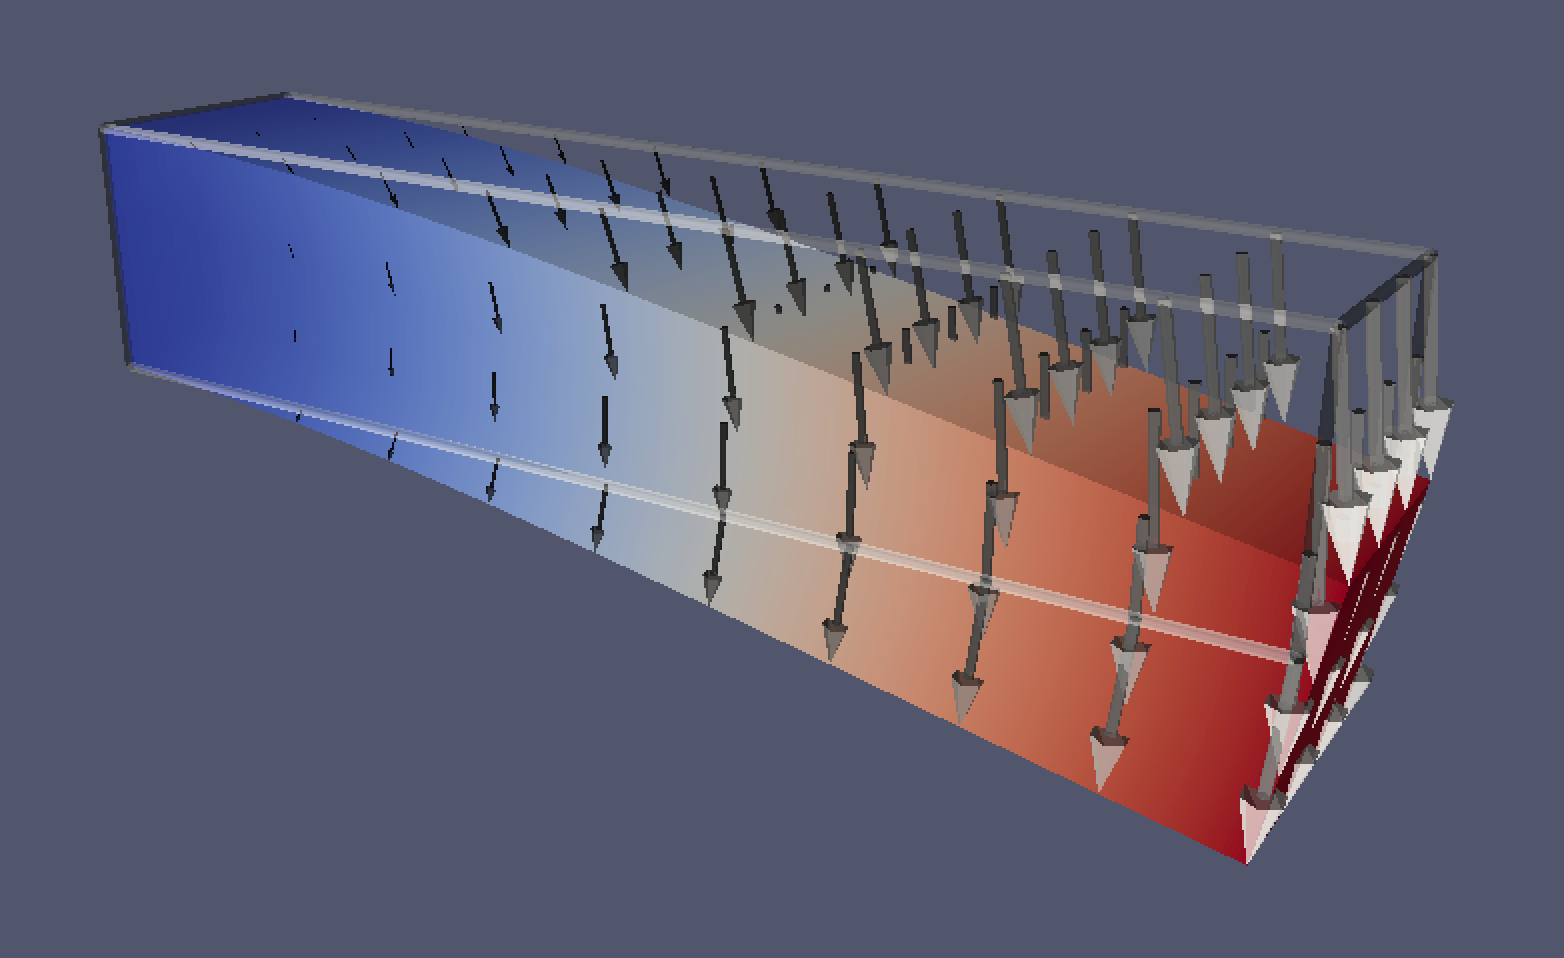
\includegraphics[width=0.95\linewidth]{fig/elasticity.png}}
  \caption{
  Plot of gravity-induced deflection in a clamped beam for the elasticity problem.
  }
\end{figure}
%\clearpage % flush figures


% !split
% Stand-alone notebook?

\section{The Navier--Stokes equations}
\label{ftut1:NS}

\index{Navier-Stokes equations}
\index{CFD}

For the next example, we will solve the incompressible Navier--Stokes
equations. This problem combines many of the challenges from our
previously studied problems: time-dependence, nonlinearity, and
vector-valued variables. We shall touch on a number of FEniCS topics,
many of them quite advanced. But you will see that even a relatively
complex algorithm such as a second-order splitting method for the
incompressible Navier--Stokes equations, can be implemented with
relative ease in FEniCS.

\subsection{PDE problem}

The incompressible Navier--Stokes equations form a system of equations
for the velocity $u$ and pressure $p$ in an incompressible fluid:

\begin{align}
  \label{ftut1:ns:momentum}
  \varrho\left(\frac{\partial u}{\partial t} +
  u \cdot \nabla u\right) &= \nabla\cdot\sigma(u, p) + f, \\
  \label{ftut1:ns:continuity}
  \nabla \cdot u &= 0.
\end{align}
The right-hand side $f$ is a given force per unit volume and
just as for the equations of linear elasticity,
$\sigma(u, p)$ denotes the stress tensor, which for a Newtonian fluid
is given by

\index{stress tensor}

\begin{equation}
  \sigma(u, p) = 2\mu\epsilon(u) - pI,
\end{equation}
where $\epsilon(u)$ is the strain-rate tensor

\index{strain-rate tensor}

\[ \epsilon(u) = \frac{1}{2}\left(\nabla u + (\nabla u)^T\right)\tp\]
The parameter $\mu$ is the dynamic viscosity. Note that the momentum
equation (\ref{ftut1:ns:momentum}) is very similar to the elasticity
equation (\ref{ftut:elast:varform:equilibrium}). The difference is in the
two additional terms $\varrho(\partial u / \partial t + u \cdot \nabla u)$ and the different
expression for the stress tensor. The two extra terms express the
acceleration balanced by the force $F = \nabla\cdot\sigma + f$ per unit volume in Newton's second law of motion.

\subsection{Variational formulation}
\label{ftut1:NS:varform}

The Navier--Stokes equations are different from
the time-dependent heat equation in that we need to solve a system of
equations and this system is of a special type. If we apply the same
technique as for the heat equation; that is, replacing the time
derivative with a simple difference quotient, we obtain a nonlinear
system of equations. This in
itself is not a problem for FEniCS as we saw in Section~\ref{ftut1:gallery:nonlinearpoisson}, but the system has a so-called
\emph{saddle point structure} and requires special techniques
(special preconditioners and iterative methods) to be solved efficiently.

\index{splitting method}
\index{Chorin's method}
\index{incremental pressure correction scheme}

Instead, we will apply a simpler and often very efficient approach,
known as a \emph{splitting method}. The idea is to
consider the two equations (\ref{ftut1:ns:momentum}) and
(\ref{ftut1:ns:continuity}) separately. There exist many splitting
strategies for the incompressible Navier--Stokes equations. One of the
oldest is the method proposed by Chorin \cite{Chorin1968} and
Temam \cite{Temam1969}, often referred to as \emph{Chorin's method}. We will
use a modified version of Chorin's method, the so-called incremental
pressure correction scheme (IPCS) due to \cite{Goda1979} which gives
improved accuracy compared to the original scheme at little extra
cost.

The IPCS scheme involves three steps. First, we compute a \emph{tentative
velocity} $u^{\star}$ by advancing the momentum equation
(\ref{ftut1:ns:momentum}) by a midpoint finite difference scheme in
time, but using the pressure $p^{n}$ from the
previous time interval. We will also linearize the nonlinear convective
term by using the known velocity $u^{n}$ from the previous time step:
$u^{n}\cdot\nabla u^{n}$.
The variational problem for this first step is

\begin{align}
\label{ftut1:ipcs1}
      & \langle {\varrho(u^{\star} - u^{n}) / \dt},{v} \rangle
      + \langle {\varrho u^{n} \cdot \nabla u^{n}},{v} \rangle
      + \nonumber
        \langle {\sigma(u^{n+\frac{1}{2}}, p^{n})},{\epsilon(v)} \rangle \\
      &\quad\quad\quad\quad\quad
      + \langle {p^{n} n},{v} \rangle_{\partial\Omega}
      - \langle {\mu\nabla u^{n+\frac{1}{2}}\cdot n},{v} \rangle_{\partial\Omega}
      = \langle {f^{n+1}},{v} \rangle.
\end{align}
This notation, suitable for problems with many terms in the variational
formulations, requires some explanation. First, we use the short-hand
notation

\[
  \inner{v}{w} = \int_{\Omega} vw \dx, \quad
  \inner{v}{w}_{\partial\Omega} = \int_{\partial\Omega} vw \ds.
\]
This allows us to express the variational problem in a more compact
way. Second, we use the notation $u^{n+\frac{1}{2}}$. This notation
refers to the value of $u$ at the midpoint of the interval, usually
approximated by an arithmetic mean:

\[
  u^{n+\frac{1}{2}} \approx (u^n + u^{n+1}) / 2.
\]
Third, we notice that the variational problem (\ref{ftut1:ipcs1})
arises from the integration by parts of the term
$\inner{-\nabla\cdot\sigma}{v}$. Just as for the elasticity problem in
Section~\ref{ftut:elast}, we obtain

\[
  \inner{-\nabla\cdot\sigma}{v}
  = \inner{\sigma}{\epsilon(v)}
  - \inner{T}{v}_{\partial\Omega},
\]
where $T = \sigma\cdot n$ is the boundary traction. If we solve a
problem with a free boundary, we can take $T = 0$ on the
boundary. However, if we compute the flow through a channel or a pipe
and want to model flow that continues into an ``imaginary channel'' at
the outflow, we need to treat this term with some care. The assumption
we then make is that the derivative of the velocity in the direction
of the channel is zero at the outflow, corresponding to a flow that is
``fully developed'' or doesn't change significantly downstream of the
outflow. Doing so, the remaining boundary term at the outflow becomes
$pn - \mu\nabla u \cdot n$, which is the term appearing in the
variational problem (\ref{ftut1:ipcs1}). Note that this argument and
the implementation depends on the exact definition of $\nabla u$, as
either the matrix with components $\partial u_i / \partial x_j$ or
$\partial u_j / \partial x_i$. We here choose the latter, $\partial
u_j / \partial x_i$, which means that we must use the FEniCS operator
\Verb!nabla_grad! for the implementation. If we use the \texttt{grad} operator and
the definition $\partial u_i / \partial x_j$, we must instead keep the
terms $pn - \mu(\nabla u)^{\top} \cdot n$!

\index{grad@{\rm\texttt{grad}}}
\index{nabla\_grad@{\rm\texttt{nabla\_grad}}}

\begin{warning_mdfboxadmon}[\texttt{grad(u)} vs. \protect\Verb!nabla\_grad(u)!]
For scalar functions, $\nabla u$ has a clear meaning as the vector

\[ \nabla u =\left(\frac{\partial u}{\partial x}, \frac{\partial u}{\partial y},
\frac{\partial u}{\partial z}\right)\tp\]
However, if $u$ is vector-valued, the meaning is less clear.
Some sources define $\nabla u$ as the matrix with elements
$\partial u_j / \partial x_i$, while other sources prefer
$\partial u_i / \partial x_j$. In FEniCS, \texttt{grad(u)} is defined as the
matrix with elements $\partial u_i / \partial x_j$, which is the
natural definition of $\nabla u$ if we think of this as the \emph{gradient} or
\emph{derivative} of $u$. This way, the matrix $\nabla u$ can be applied to
a differential $\dx$ to give an increment $\mathrm{d}u = \nabla u \,
\dx$. Since the alternative interpretation of $\nabla u$ as the matrix
with elements $\partial u_j / \partial x_i$ is very common, in
particular in continuum mechanics, FEniCS
provides the operator \Verb!nabla_grad! for this purpose.
For the Navier--Stokes equations, it is important to consider the
term $u \cdot \nabla u$ which should be interpreted as the vector
$w$ with elements
$w_i = \sum_j \left(u_j \frac{\partial}{\partial x_j}\right) u_i
     = \sum_j u_j \frac{\partial u_i}{\partial x_j}$.
This term can be implemented in FEniCS either as
\texttt{grad(u)*u}, since this is expression becomes
$\sum_j \partial u_i/\partial x_j u_j$, or as
\Verb!dot(u, nabla_grad(u))! since this expression becomes
$\sum_i u_i \partial u_j/\partial x_i$. We will use the notation
\Verb!dot(u, nabla_grad(u))! below since it corresponds more closely
to the standard notation $u \cdot \nabla u$.

To be more precise, there are three different notations used for PDEs
involving gradient, divergence, and curl operators.  One employs
$\mathrm{grad}\, u$, $\mathrm{div}\, u$, and $\mathrm{curl}\, u$
operators. Another employs $\nabla u$ as a synonym for
$\mathrm{grad}\, u$, $\nabla\cdot u$ means $\mathrm{div}\, u$, and
$\nabla\times u$ is the name for $\mathrm{curl}\, u$. The third
operates with $\nabla u$, $\nabla\cdot u$, and $\nabla\times u$ in
which $\nabla$ is a \emph{vector} and, e.g., $\nabla u$ is a dyadic
expression: $(\nabla u)_{i,j} = \partial u_j/\partial x_i =
(\mathrm{grad}\,u)^{\top}$. The latter notation, with $\nabla$ as a
vector operator, is often handy when deriving equations in continuum
mechanics, and if this interpretation of $\nabla$ is the foundation of
your PDE, you must use \Verb!nabla_grad!, \Verb!nabla_div!, and \Verb!nabla_curl! in
FEniCS code as these operators are compatible with dyadic
computations.  From the Navier--Stokes equations we can easily see
what $\nabla$ means: if the convective term has the form $u\cdot
\nabla u$, actually meaning $(u\cdot\nabla) u$, then $\nabla$ is a
vector and the implementation becomes \Verb!dot(u, nabla_grad(u))! in
FEniCS, but if we see $\nabla u\cdot u$ or $(\mathrm{grad} u)\cdot u$,
the corresponding FEniCS expression is \texttt{dot(grad(u), u)}.

Similarly, the divergence of a tensor field like the stress tensor
$\sigma$ can also be expressed in two different ways, as either
\texttt{div(sigma)} or \Verb!nabla_div(sigma)!. The first case corresponds to the
components $\partial \sigma_{ij}/{\partial x_j}$ and the second to
$\partial \sigma_{ij}/{\partial x_i}$. In general, these expressions
will be different but when the stress measure is symmetric, the
expressions have the same value.
\end{warning_mdfboxadmon} % title: \texttt{grad(u)} vs. \protect\Verb!nabla\_grad(u)!

We now move on to the second step in our splitting scheme for the
incompressible Navier--Stokes equations. In the first step, we computed
the tentative velocity $u^{\star}$ based on the pressure from the
previous time step. We may now use the computed tentative velocity to
compute the new pressure $p^n$:

\begin{equation}
\label{ftut1:ipcs2}
  \langle \nabla p^{n+1}, \nabla q \rangle
  = \langle {\nabla p^{n}},{\nabla q} \rangle
  - \dt^{-1} \langle{\nabla \cdot u^{\star}},{q} \rangle.
\end{equation}
Note here that $q$ is a scalar-valued test function from the pressure
space, whereas the test function $v$ in (\ref{ftut1:ipcs1}) is a
vector-valued test function from the velocity space.

One way to think about this step is to subtract the Navier--Stokes
momentum equation (\ref{ftut1:ns:momentum}) expressed in terms of the
tentative velocity $u^{\star}$ and the pressure $p^n$ from the
momentum equation expressed in terms of the velocity $u^{n+1}$ and
pressure $p^{n+1}$. This results in the equation

\begin{equation} \label{ftut1:ipcs:step}
  (u^{n+1} - u^{\star}) / \dt + \nabla p^{n+1} - \nabla p^n = 0.
\end{equation}
Taking the divergence and requiring that $\nabla \cdot u^{n+1} = 0$ by the
Navier--Stokes continuity equation (\ref{ftut1:ns:continuity}), we
obtain the equation $-\nabla\cdot u^{\star} / \dt + \nabla^2 p^{n+1} -
\nabla^2 p^n = 0$, which is a Poisson problem for the pressure $p^{n+1}$
resulting in the variational problem (\ref{ftut1:ipcs2}).

Finally, we compute the corrected velocity $u^{n+1}$ from the equation
(\ref{ftut1:ipcs:step}). Multiplying this equation by a test function
$v$, we obtain

\begin{equation}
\label{ftut1:ipcs3}
  \langle {u^{n+1}},{v} \rangle
  =
  \langle {u^{\star}},{v} \rangle
  - \dt \langle {\nabla(p^{n+1}-p^{n})},{v} \rangle.
\end{equation}

In summary, we may thus solve the incompressible Navier--Stokes
equations efficiently by solving a sequence of three linear variational
problems in each time step.

\subsection{FEniCS implementation}

\paragraph{Test problem 1: Channel flow.}
\index{channel flow}

As a first test problem, we compute the flow between two infinite
plates, so-called channel or Poiseuille flow. As we shall see, this
problem has a known analytical solution. Let $H$ be the distance
between the plates and $L$ the length of the channel. There are no
body forces.

\index{scaling}

We may scale the problem first to get rid of seemingly independent
physical parameters. The physics of this problem is governed by
viscous effects only, in the direction perpendicular to the flow, so a
time scale should be based on diffusion accross the channel: $t_c =
H^2/\nu$. We let $U$, some characteristic inflow velocity, be the
velocity scale and $H$ the spatial scale. The pressure scale is taken
as the characteristic shear stress, $\mu U/H$, since this is a primary
example of shear flow.  Inserting $\bar x = x/H$, $\bar y = y/H$,
$\bar z = z/H$, $\bar u =u/U$, $\bar p = Hp/(\mu U)$, and $\bar t =
H^2/\nu$ in the equations results in the scaled Navier--Stokes
equations (dropping bars after the scaling):

\index{Reynolds number}

\begin{align*}
\frac{\partial u}{\partial t} + \mathrm{Re}\, u\cdot\nabla u
&= -\nabla p + \nabla^2 u,\\
\nabla\cdot u &= 0\tp
\end{align*}
Here, $\mathrm{Re} = \varrho UH/\mu$ is the Reynolds number. Because
of the time and pressure scales, which are different from
convection-dominated fluid flow, the Reynolds number is associated
with the convective term and not the viscosity term.

The exact solution is derived by assuming $u=(u_x(x,y,z),0,0)$, with
the $x$ axis pointing along the channel. Since $\nabla\cdot u=0$, $u$
cannot depend on $x$. The physics of channel flow is also
two-dimensional so we can omit the $z$ coordinate (more precisely:
$\partial/\partial z=0$). Inserting $u=(u_x,0,0)$ in the (scaled)
governing equations gives $u_x''(y) = \partial p/\partial x$.
Differentiating this equation with respect to $x$ shows that $\partial^2
p/\partial^2 x =0$ so $\partial
p/\partial x$ is a constant, here called $-\beta$. This is the driving
force of the flow and can be specified as a known parameter in the
problem.  Integrating $u_x''(y)=-\beta$ over the width of the channel,
$[0,1]$, and requiring $u=(0, 0, 0)$ at the channel walls, results in
$u_x=\frac{1}{2}\beta y(1-y)$. The characteristic inlet velocity
$U$ can be taken as the maximum inflow at $y=1/2$, implying
$\beta = 8$. The length of the channel, $L/H$ in the scaled
model, has no impact on the result, so for simplicity we just compute
on the unit square. Mathematically, the pressure must be prescribed
at a point, but since $p$ does not depend on $y$, we can set $p$ to a
known value, e.g.~zero, along the outlet boundary $x=1$. The result
is $p(x)=8(1-x)$ and $u_x=4y(1-y)$.

The boundary conditions can be set as $p=8$ at $x=0$, $p=0$ at $x=1$
and $u=(0, 0, 0)$ on the walls $y=0,1$. This defines the pressure drop
and should result in unit maximum velocity at the inlet and outlet and
a parabolic velocity profile without further specifications. Note that
it is only meaningful to solve the Navier--Stokes equations in 2D or
3D geometries, although the underlying mathematical problem collapses
to two 1D problems, one for $u_x(y)$ and one for $p(x)$.

The scaled model is not so easy to simulate using a standard
Navier--Stokes solver with dimensions. However, one can argue that the
convection term is zero, so the Re coefficient in front of this term
in the scaled PDEs is not important and can be set to unity. In that
case, setting $\varrho = \mu = 1$ in the original Navier--Stokes equations
resembles the scaled model.

For a specific engineering problem one wants to simulate a specific
fluid and set corresponding parameters. A general solver is therefore
most naturally implemented with dimensions and the original physical
parameters. However, scaling may greatly simplify numerical
simulations. First of all, it shows that all fluids behave in the
same way: it does not matter whether we have oil, gas, or water
flowing between two plates, and it does not matter how fast the flow
is (up to some criticial value of the Reynolds number where the flow
becomes unstable and transitions to a complicated turbulent flow of
totally different nature). This means that one simulation is enough
to cover all types of channel flow! In other applications, scaling
shows that it might be necessary to set just the fraction of some
parameters (dimensionless numbers) rather than the parameters
themselves. This simplifies exploring the input parameter space which
is often the purpose of simulation. Frequently, the scaled problem is
run by setting some of the input parameters with dimension to fixed
values (often unity).

\paragraph{FEniCS implementation.}
Our previous examples have all started out with the creation of a mesh
and then the definition of a \texttt{FunctionSpace} on the mesh. For the
Navier--Stokes splitting scheme we will need to define two function
spaces, one for the velocity and one for the pressure:

\begin{lstlisting}[language=Python,style=graycolor]
V = VectorFunctionSpace(mesh, 'P', 2)
Q = FunctionSpace(mesh, 'P', 1)
\end{lstlisting}
The first space \texttt{V} is a vector-valued function space for the velocity
and the second space \texttt{Q} is a scalar-valued function space for the
pressure. We use piecewise quadratic elements for the velocity and
piecewise linear elements for the pressure. When creating a
\texttt{VectorFunctionSpace} in FEniCS, the value-dimension (the length of
the vectors) will be set equal to the geometric dimension of the
finite element mesh. One can easily create vector-valued function
spaces with other dimensions in FEniCS by adding the keyword parameter
\texttt{dim}:

\index{VectorFunctionSpace@{\rm\texttt{VectorFunctionSpace}}}

\begin{lstlisting}[language=Python,style=graycolor]
V = VectorFunctionSpace(mesh, 'P', 2, dim=10)
\end{lstlisting}


\begin{notice_mdfboxadmon}[Stable finite element spaces for the Navier--Stokes equations]
It is well-known that certain finite element spaces are not \emph{stable}
for the Navier--Stokes equations, or even for the simpler Stokes
equations. The prime example of an unstable pair of finite element
spaces is to use first degree continuous piecewise polynomials for both the
velocity and the pressure. Using an
unstable pair of spaces typically results in a solution with
\emph{spurious} (unwanted, non-physical) oscillations in the pressure
solution. The simple remedy is to use continuous piecewise
quadratic elements for the velocity and continuous piecewise linear
elements for the pressure. Together, these elements form the so-called
\emph{Taylor-Hood} element. Spurious oscillations may occur also for
splitting methods if an unstable element pair is used.
\end{notice_mdfboxadmon} % title: Stable finite element spaces for the Navier--Stokes equations



Since we have two different function spaces, we need to create two sets
of trial and test functions:

\begin{lstlisting}[language=Python,style=graycolor]
u = TrialFunction(V)
v = TestFunction(V)
p = TrialFunction(Q)
q = TestFunction(Q)
\end{lstlisting}

\index{near@{\rm\texttt{near}}}

As we have seen in previous examples, boundaries may be defined in
FEniCS by defining Python functions that return \texttt{True} or \texttt{False}
depending on whether a point should be considered part of the
boundary, for example

\begin{lstlisting}[language=Python,style=graycolor]
def boundary(x, on_boundary):
    return near(x[0], 0)
\end{lstlisting}
This function defines the boundary to be all points with
$x$-coordinate equal to (near) zero. The \texttt{near} function comes from
FEniCS and performs a test with tolerance: \texttt{abs(x[0] - 0) < 3E-16} so we
do not run into rounding troubles.  Alternatively, we may give the
boundary definition as a string of C++ code, much like we have
previously defined expressions such as \Verb!u_D = Expression('1 + x[0]*x[0] + 2*x[1]*x[1]', degree=2)!. The above definition of the boundary in
terms of a Python function may thus be replaced by a simple C++
string:

\begin{lstlisting}[language=Python,style=graycolor]
boundary = 'near(x[0], 0)'
\end{lstlisting}
This has the advantage of moving the computation of which nodes
belong to the boundary from Python to C++, which improves the efficiency
of the program.

For the current example, we will set three different boundary
conditions. First, we will set $u = 0$ at the walls of the channel;
that is, at $y = 0$ and $y = 1$. Second, we will set $p = 8$ at the
inflow ($x = 0$) and, finally, $p = 0$ at the outflow ($x = 1$). This
will result in a pressure gradient that will accelerate the flow from
the initial state with zero velocity. These boundary conditions may be
defined as follows:

\begin{lstlisting}[language=Python,style=graycolor]
# Define boundaries
inflow   = 'near(x[0], 0)'
outflow  = 'near(x[0], 1)'
walls    = 'near(x[1], 0) || near(x[1], 1)'

# Define boundary conditions
bcu_noslip  = DirichletBC(V, Constant((0, 0)), walls)
bcp_inflow  = DirichletBC(Q, Constant(8), inflow)
bcp_outflow = DirichletBC(Q, Constant(0), outflow)
bcu = [bcu_noslip]
bcp = [bcp_inflow, bcp_outflow]
\end{lstlisting}

At the end, we collect the boundary conditions for the velocity and
pressure in Python lists so we can easily access them in the
following computation.

We now move on to the definition of the variational forms. There are
three variational problems to be defined, one for each step in the
IPCS scheme. Let us look at the definition of the first variational
problem. We start with some constants:

\begin{lstlisting}[language=Python,style=graycolor]
U   = 0.5*(u_n + u)
n   = FacetNormal(mesh)
f   = Constant((0, 0))
k   = Constant(dt)
mu  = Constant(mu)
rho = Constant(rho)
\end{lstlisting}

The next step is to set up the variational form for the first step
(\ref{ftut1:ipcs1}) in the solution process.  Since the variational
problem contains a mix of known and unknown quantities we will use the
following naming convention: \texttt{u} is the unknown (mathematically
$u^{n+1}$) as a trial function in the variational form, \Verb!u_! is the
most recently computed approximation ($u^{n+1}$ available as a
\texttt{Function} object), \Verb!u_n! is $u^n$, and the same convention goes for
\texttt{p}, \Verb!p_! ($p^{n+1}$), and \Verb!p_n! ($p^n$).

\begin{lstlisting}[language=Python,style=graycolor]
# Define strain-rate tensor
def epsilon(u):
    return sym(nabla_grad(u))

# Define stress tensor
def sigma(u, p):
    return 2*mu*epsilon(u) - p*Identity(len(u))

# Define variational problem for step 1
F1 = rho*dot((u - u_n) / k, v)*dx + \
     rho*dot(dot(u_n, nabla_grad(u_n)), v)*dx \
   + inner(sigma(U, p_n), epsilon(v))*dx \
   + dot(p_n*n, v)*ds - dot(mu*nabla_grad(U)*n, v)*ds \
   - dot(f, v)*dx
a1 = lhs(F1)
L1 = rhs(F1)
\end{lstlisting}

Note that we take advantage of the Python programming language to
define our own operators \texttt{sigma} and \texttt{epsilon}. Using Python this way
makes it easy to extend the mathematical language of FEniCS with
special operators and constitutive laws.

Also note that FEniCS can sort out the bilinear form $a(u,v)$ and
linear form $L(v)$ forms by the \texttt{lhs}
and \texttt{rhs} functions. This is particularly convenient in longer and
more complicated variational forms.

The splitting scheme requires the solution of a sequence of three
variational problems in each time step. We have previously used the
built-in FEniCS function \texttt{solve} to solve variational problems. Under
the hood, when a user calls \texttt{solve(a == L, u, bc)}, FEniCS will
perform the following steps:

\begin{lstlisting}[language=Python,style=graycolor]
A = assemble(A)
b = assemble(L)
bc.apply(A, b)
solve(A, u.vector(), b)
\end{lstlisting}
In the last step, FEniCS uses the overloaded \texttt{solve} function to solve
the linear system \texttt{AU = b} where \texttt{U} is the vector of degrees of
freedom for the function $u(x) = \sum_{j=1} U_j \phi_j(x)$.

\index{linear system}

In our implementation of the splitting scheme, we will make use of
these low-level commands to first assemble and then call solve. This
has the advantage that we may control when we assemble and when we
solve the linear system. In particular, since the matrices for the
three variational problems are all time-independent, it makes sense to
assemble them once and for all outside of the time-stepping loop:

\index{assemble@{\rm\texttt{assemble}}}

\begin{lstlisting}[language=Python,style=graycolor]
A1 = assemble(a1)
A2 = assemble(a2)
A3 = assemble(a3)
\end{lstlisting}
Within the time-stepping loop, we may then assemble only the
right-hand side vectors, apply boundary conditions, and call the solve
function as here for the first of the three steps:

\begin{lstlisting}[language=Python,style=graycolor]
# Time-stepping
t = 0
for n in range(num_steps):

    # Update current time
    t += dt

    # Step 1: Tentative velocity step
    b1 = assemble(L1)
    [bc.apply(b1) for bc in bcu]
    solve(A1, u_.vector(), b1)
\end{lstlisting}
Notice the Python \emph{list comprehension} \texttt{[bc.apply(b1) for bc in bcu]}
which iterates over all \texttt{bc} in the list \texttt{bcu}. This is a convenient
and compact way to construct a loop that applies
all boundary conditions in a single line. Also, the code works if
we add more Dirichlet boundary conditions in the future. Note that
the boundary conditions only need to be applied to the right-hand side
vectors as they have already been applied to the matrices (not shown).

Finally, let us look at an important detail in how we use parameters
such as the time step \texttt{dt} in the definition of our variational
problems. Since we might want to change these later, for example if we
want to experiment with smaller or larger time steps, we wrap these
using a FEniCS \texttt{Constant}:

\begin{lstlisting}[language=Python,style=graycolor]
k = Constant(dt)
\end{lstlisting}

The assembly of matrices and vectors in FEniCS is based on code
generation. This means that whenever we change a variational problem,
FEniCS will have to generate new code, which may take a little
time. New code will also be generated and compiled when a float value
for the time step is changed. By wrapping this parameter using
\texttt{Constant}, FEniCS will treat the parameter as a generic constant and
not as a specific numerical value, which prevents repeated code
generation. In the case of the time step, we choose a new name \texttt{k}
instead of \texttt{dt} for the \texttt{Constant} since we also want to use the
variable \texttt{dt} as a Python float as part of the time-stepping.

The complete code for simulating 2D channel flow with FEniCS
can be found in the file \href{{https://fenicsproject.org/pub/tutorial/python/vol1/ft07_navier_stokes_channel.py}}{\nolinkurl{ft07_navier_stokes_channel.py}}.

\index{ft07\_navier\_stokes\_channel.py@{\rm\texttt{ft07\_navier\_stokes\_channel.py}}}

\paragraph{Verification.}
\index{verification}

We compute the error at the nodes as we have done before to verify
that our implementation is correct. Our Navier--Stokes solver computes
the solution to the time-dependent incompressible Navier--Stokes
equations, starting from the initial condition $u = (0, 0)$. We have
not specified the initial condition explicitly in our solver which
means that FEniCS will initialize all variables, in particular the
previous and current velocities \Verb!u_n! and \Verb!u_!, to zero. Since the
exact solution is quadratic, we expect the solution to be exact to
within machine precision at the nodes at infinite time. For our
implementation, the error quickly approaches zero and is approximately
$10^{-6}$ at time $T = 10$.


\begin{figure}[!ht]  % ftut1:fig:navier_stokes_channel
  \centerline{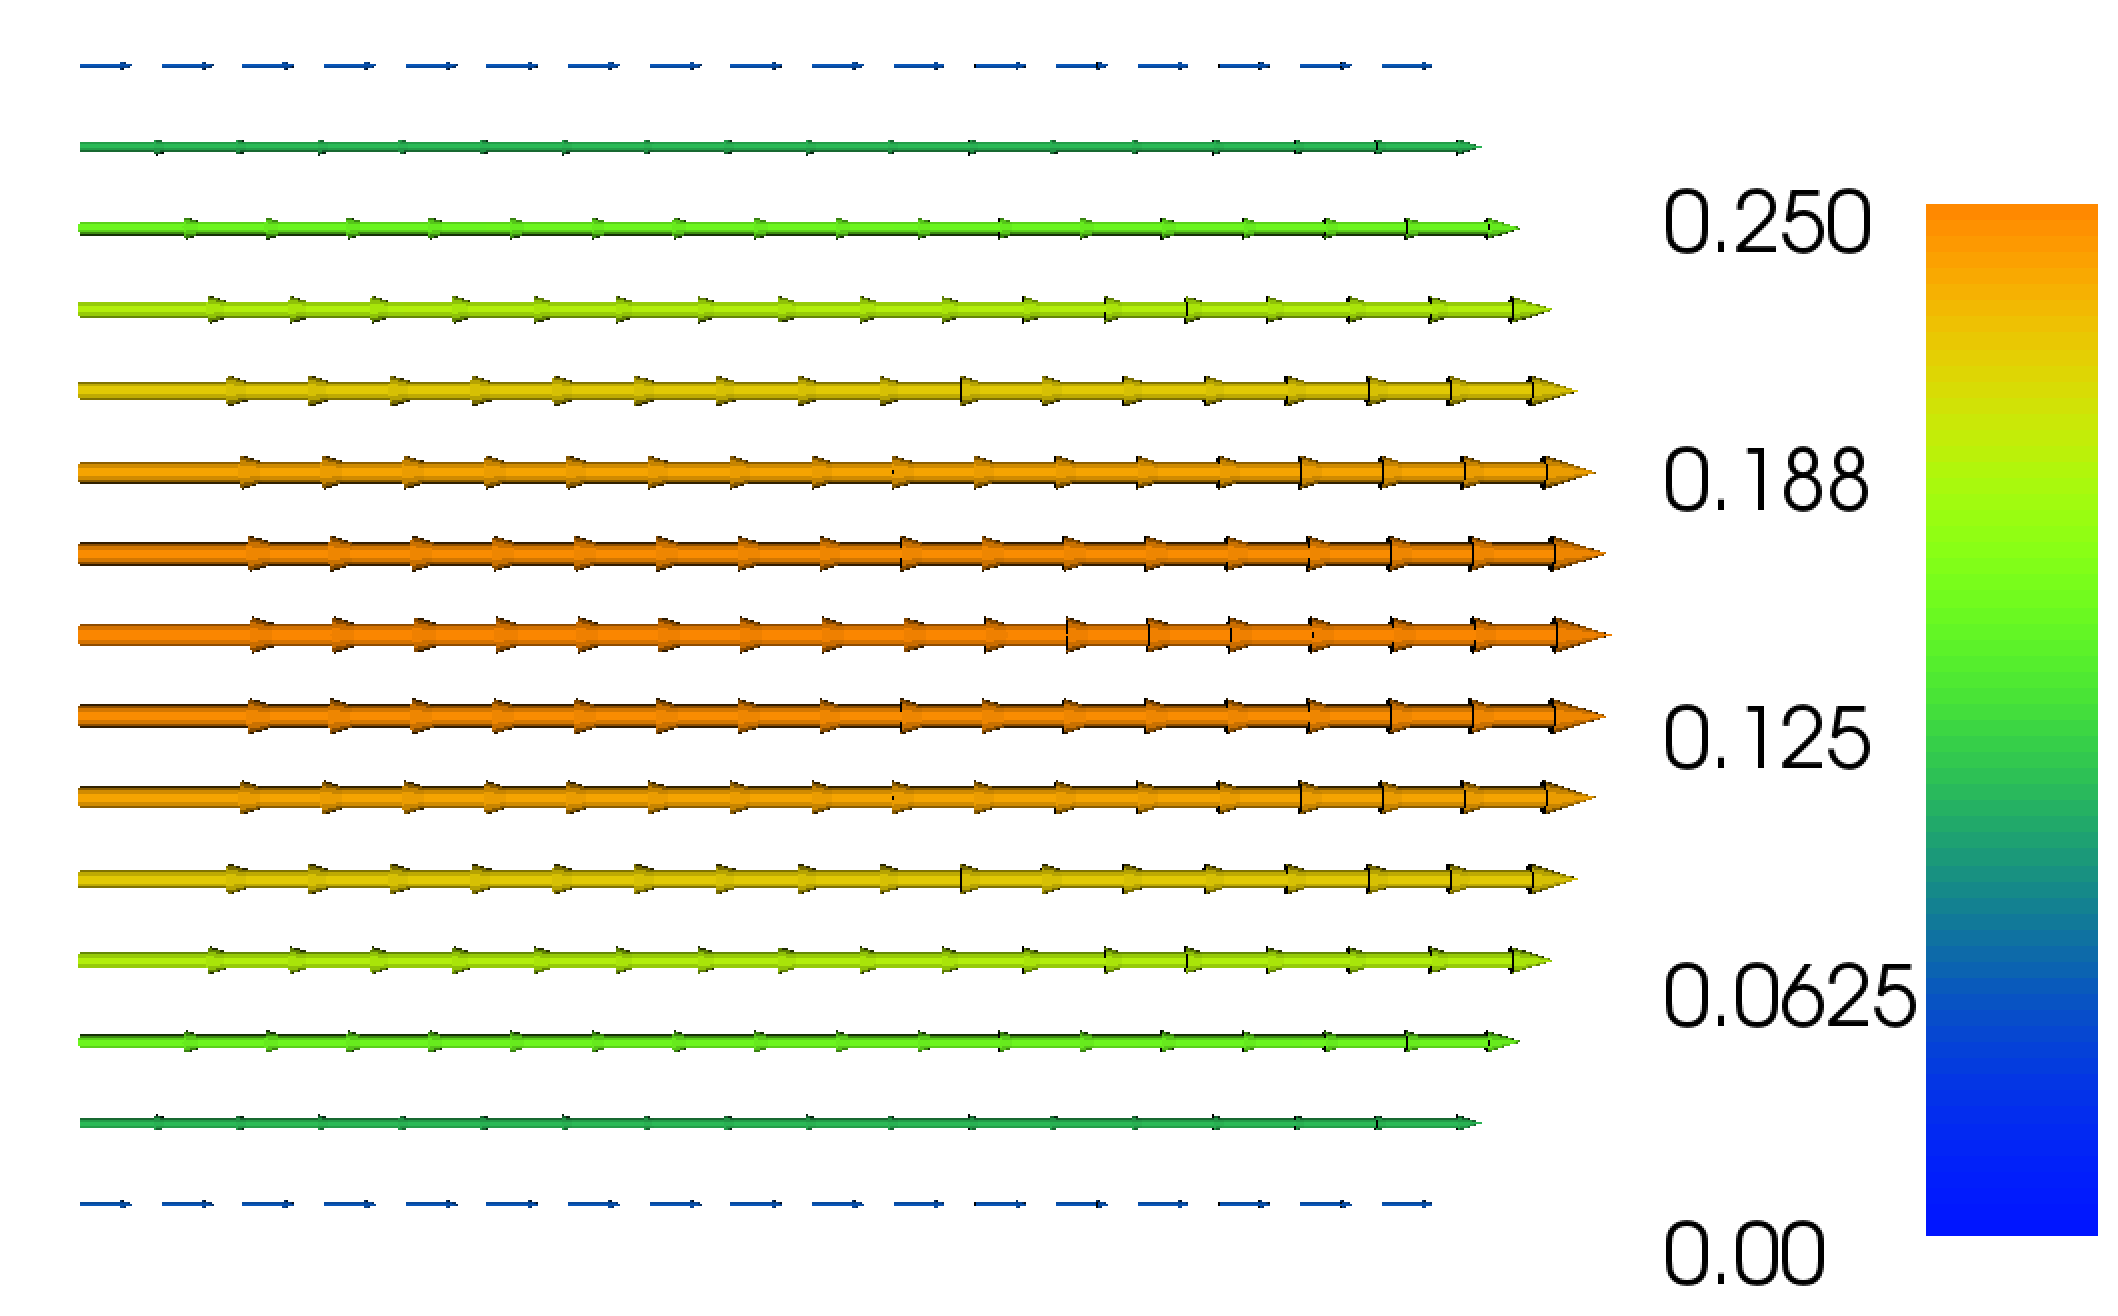
\includegraphics[width=0.95\linewidth]{fig/navier_stokes_channel.png}}
  \caption{
  Plot of the velocity profile at the final time for the Navier--Stokes channel flow example. \label{ftut1:fig:navier_stokes_channel}
  }
\end{figure}
%\clearpage % flush figures ftut1:fig:navier_stokes_channel



\paragraph{Test problem 2: Flow past a cylinder.}
\index{cylinder flow}

We now turn our attention to a more challenging problem: flow
past a circular cylinder. The geometry and parameters are taken from
problem DFG 2D-2 in the \href{{http://www.featflow.de/en/benchmarks/cfdbenchmarking/flow/dfg_benchmark2_re100.html}}{FEATFLOW/1995-DFG benchmark suite}\footnote{\texttt{http://www.featflow.de/en/benchmarks/cfdbenchmarking/flow/dfg\_benchmark2\_re100.html}}
and is illustrated in Figure~\ref{ftut1:navier_stokes_cylinder:geometry}. The kinematic viscosity is
given by $\nu = 0.001 = \mu/\varrho$ and the inflow velocity profile is
specified as

\[
  u(x, y, t) = \left(1.5 \cdot \frac{4y(0.41 - y)}{0.41^2}, 0\right),
\]
which has a maximum magnitude of $1.5$ at $y = 0.41/2$. We do not
use any scaling for this problem since all exact parameters are known.


\begin{figure}[!ht]  % ftut1:navier_stokes_cylinder:geometry
  \centerline{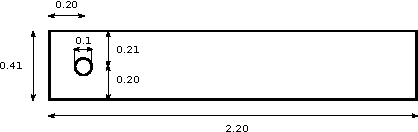
\includegraphics[width=0.95\linewidth]{fig/navier_stokes_cylinder_geometry.pdf}}
  \caption{
  Geometry for the flow past a cylinder test problem. Notice the slightly perturbed and unsymmetric geometry. \label{ftut1:navier_stokes_cylinder:geometry}
  }
\end{figure}
%\clearpage % flush figures ftut1:navier_stokes_cylinder:geometry

\paragraph{FEniCS implementation.}
So far all our domains have been simple shapes such as a unit square or
a rectangular box. A number of such simple meshes may be created
using the built-in mesh classes in FEniCS
(\texttt{UnitIntervalMesh},
\texttt{UnitSquareMesh},
\texttt{UnitCubeMesh},
\texttt{IntervalMesh},
\texttt{RectangleMesh},
\texttt{BoxMesh}).
FEniCS supports the creation of more complex meshes via a technique
called \emph{constructive solid geometry} (CSG), which lets us define
geometries in terms of simple shapes (primitives) and set operations:
union, intersection, and set difference. The set operations are
encoded in FEniCS using the operators \texttt{+} (union), \texttt{*} (intersection),
and \texttt{-} (set difference). To access the CSG functionality in FEniCS,
one must import the FEniCS module \texttt{mshr} which provides the
extended meshing functionality of FEniCS.

\index{mshr}
\index{CSG}
\index{constructive solid geometry}

The geometry for the cylinder flow test problem can be defined easily
by first defining the rectangular channel and then subtracting the
circle:

\begin{lstlisting}[language=Python,style=graycolor]
channel = Rectangle(Point(0, 0), Point(2.2, 0.41))
cylinder = Circle(Point(0.2, 0.2), 0.05)
domain = channel - cylinder
\end{lstlisting}
We may then create the mesh by calling the function \Verb!generate_mesh!:

\begin{lstlisting}[language=Python,style=graycolor]
mesh = generate_mesh(domain, 64)
\end{lstlisting}
Here the argument \texttt{64} indicates that we want to resolve the geometry
with 64 cells across its diameter (the channel length).

\index{generate\_mesh@{\rm\texttt{generate\_mesh}}}

To solve the cylinder test problem, we only need to make a few minor
changes to the code we wrote for the channel flow test
case. Besides defining the new mesh, the only change we need to make
is to modify the boundary conditions and the time step size. The
boundaries are specified as follows:

\begin{lstlisting}[language=Python,style=graycolor]
inflow   = 'near(x[0], 0)'
outflow  = 'near(x[0], 2.2)'
walls    = 'near(x[1], 0) || near(x[1], 0.41)'
cylinder = 'on_boundary && x[0]>0.1 && x[0]<0.3 && x[1]>0.1 && x[1]<0.3'
\end{lstlisting}
The last line may seem cryptic before you catch the idea: we want to pick
out all boundary points (\Verb!on_boundary!) that also lie within the 2D
domain $[0.1,0.3]\times [0.1,0.3]$, see Figure~\ref{ftut1:navier_stokes_cylinder:geometry}. The only possible points are then the points on the
circular boundary!

\index{set\_log\_level@{\rm\texttt{set\_log\_level}}}
\index{DEBUG@{\rm\texttt{DEBUG}} log level}
\index{PROGRESS@{\rm\texttt{PROGRESS}} log level}

In addition to these essential changes, we will make a number of small
changes to improve our solver. First, since we need to choose a
relatively small time step to compute the solution (a time step that
is too large will make the solution blow up) we add a progress bar so
that we can follow the progress of our computation. This can be done
as follows:

\index{Progress@{\rm\texttt{Progress}}}

\begin{lstlisting}[language=Python,style=graycolor]
progress = Progress('Time-stepping')
set_log_level(PROGRESS)

# Time-stepping
t = 0.0
for n in range(num_steps):

    # Update current time
    t += dt

    # Place computation here

    # Update progress bar
    progress.update(t / T)
\end{lstlisting}

\begin{notice_mdfboxadmon}[Log levels and printing in FEniCS]
Notice the call to \Verb!set_log_level(PROGRESS)! which is essential to
make FEniCS actually display the progress bar. FEniCS is actually
quite informative about what is going on during a computation but the
amount of information printed to screen depends on the current log
level. Only messages with a priority higher than or equal to the
current log level will be displayed. The predefined log levels in
FEniCS are
\texttt{DBG},
\texttt{TRACE},
\texttt{PROGRESS},
\texttt{INFO},
\texttt{WARNING},
\texttt{ERROR}, and
\texttt{CRITICAL}. By default, the log level is set to \texttt{INFO} which means
that messages at level \texttt{DBG}, \texttt{TRACE}, and \texttt{PROGRESS} will not be
printed. Users may print messages using the FEniCS functions \texttt{info},
\texttt{warning}, and \texttt{error} which will print messages at the obvious log
level (and in the case of \texttt{error} also throw an exception and
exit). One may also use the call \texttt{log(level, message)} to print a
message at a specific log level.
\end{notice_mdfboxadmon} % title: Log levels and printing in FEniCS

Since the system(s) of linear equations are significantly larger than
for the simple channel flow test problem, we choose to use an
iterative method instead of the default direct (sparse) solver used by
FEniCS when calling \texttt{solve}. Efficient solution of linear systems
arising from the discretization of PDEs requires the choice of both a
good iterative (Krylov subspace) method and a good
preconditioner. For this problem, we will simply use the biconjugate
gradient stabilized method (BiCGSTAB) and the conjugate gradient method. This can be done by adding the
keywords \texttt{bicgstab} or \texttt{cg} in the call to \texttt{solve}. We also specify
suitable preconditioners to speed up the computations:

\index{Krylov solver}
\index{preconditioner}

\begin{lstlisting}[language=Python,style=graycolor]
solve(A1, u1.vector(), b1, 'bicgstab', 'hypre_amg')
solve(A2, p1.vector(), b2, 'bicgstab', 'hypre_amg')
solve(A3, u1.vector(), b3, 'cg', 'sor')
\end{lstlisting}

Finally, to be able to postprocess the computed solution in ParaView,
we store the solution to a file in each time step. We have previously
created files with the suffix \texttt{.pvd} for this purpose. In the example
program
\href{{https://fenicsproject.org/pub/tutorial/python/vol1/ft04_heat_gaussian.py}}{\nolinkurl{ft04_heat_gaussian.py}},
we first created a file named \Verb!heat_gaussian/solution.pvd! and then
saved the solution in each time step using
\begin{lstlisting}[language=Python,style=graycolor]
vtkfile << (u, t)
\end{lstlisting}

For the present example, we will instead choose to save the solution
to XDMF format. This file format works similarly to the \texttt{.pvd} files
we have seen earlier but has several advantages. First, the storage is
much more efficient, both in terms of speed and file sizes. Second,
\texttt{.xdmf} files work in parallell, both for writing and reading
(postprocessing). Much like \texttt{.pvd} files, the actual data will not be
stored in the \texttt{.xdmf} file itself, but will instead be stored in a
(single) separate data file with the suffix \texttt{.hdf5} which is an
advanced file format designed for high-performance computing.
We create the XDMF files as follows:

\begin{lstlisting}[language=Python,style=graycolor]
xdmffile_u = XDMFFile('navier_stokes_cylinder/velocity.xdmf')
xdmffile_p = XDMFFile('navier_stokes_cylinder/pressure.xdmf')
\end{lstlisting}
In each time step, we may then store the velocity and pressure by
\begin{lstlisting}[language=Python,style=graycolor]
xdmffile_u.write(u, t)
xdmffile_p.write(p, t)
\end{lstlisting}

\index{TimeSeries@{\rm\texttt{TimeSeries}}}
\index{HDF5 format}
\index{XDMF format}
\index{.hdf5@{\rm\texttt{.hdf5}} file}
\index{.xdmf@{\rm\texttt{.xdmf}} file}

We also store the solution using a FEniCS \texttt{TimeSeries}. This allows us
to store the solution not for visualization, but for later reuse in a
computation as we will see in the next section. Using a \texttt{TimeSeries}
it is easy and efficient to read in solutions from certain points in
time during a simulation. The \texttt{TimeSeries} class also uses the HDF5
file format for efficient storage and access to data.

Figures~\ref{ftut1:fig:navier_stokes_cylinder:velocity} and~\ref{ftut1:fig:navier_stokes_cylinder:pressure} show the velocity and
pressure at final time visualized in ParaView. For the visualization
of the velocity, we have used the \textbf{Glyph} filter to visualize the
vector velocity field. For the visualization of the pressure, we have
used the \textbf{Warp By Scalar} filter.


\begin{figure}[!ht]  % ftut1:fig:navier_stokes_cylinder:velocity
  \centerline{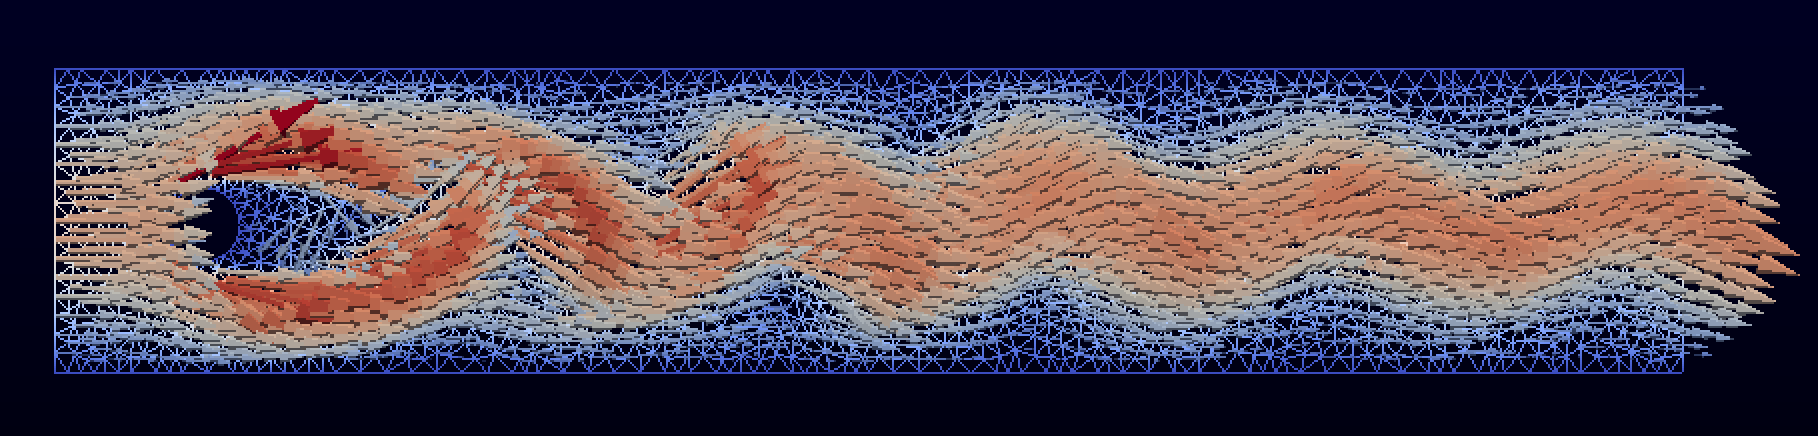
\includegraphics[width=0.95\linewidth]{fig/navier_stokes_cylinder_velocity.png}}
  \caption{
  Plot of the velocity for the cylinder test problem at final time. \label{ftut1:fig:navier_stokes_cylinder:velocity}
  }
\end{figure}
%\clearpage % flush figures ftut1:fig:navier_stokes_cylinder:velocity



\begin{figure}[!ht]  % ftut1:fig:navier_stokes_cylinder:pressure
  \centerline{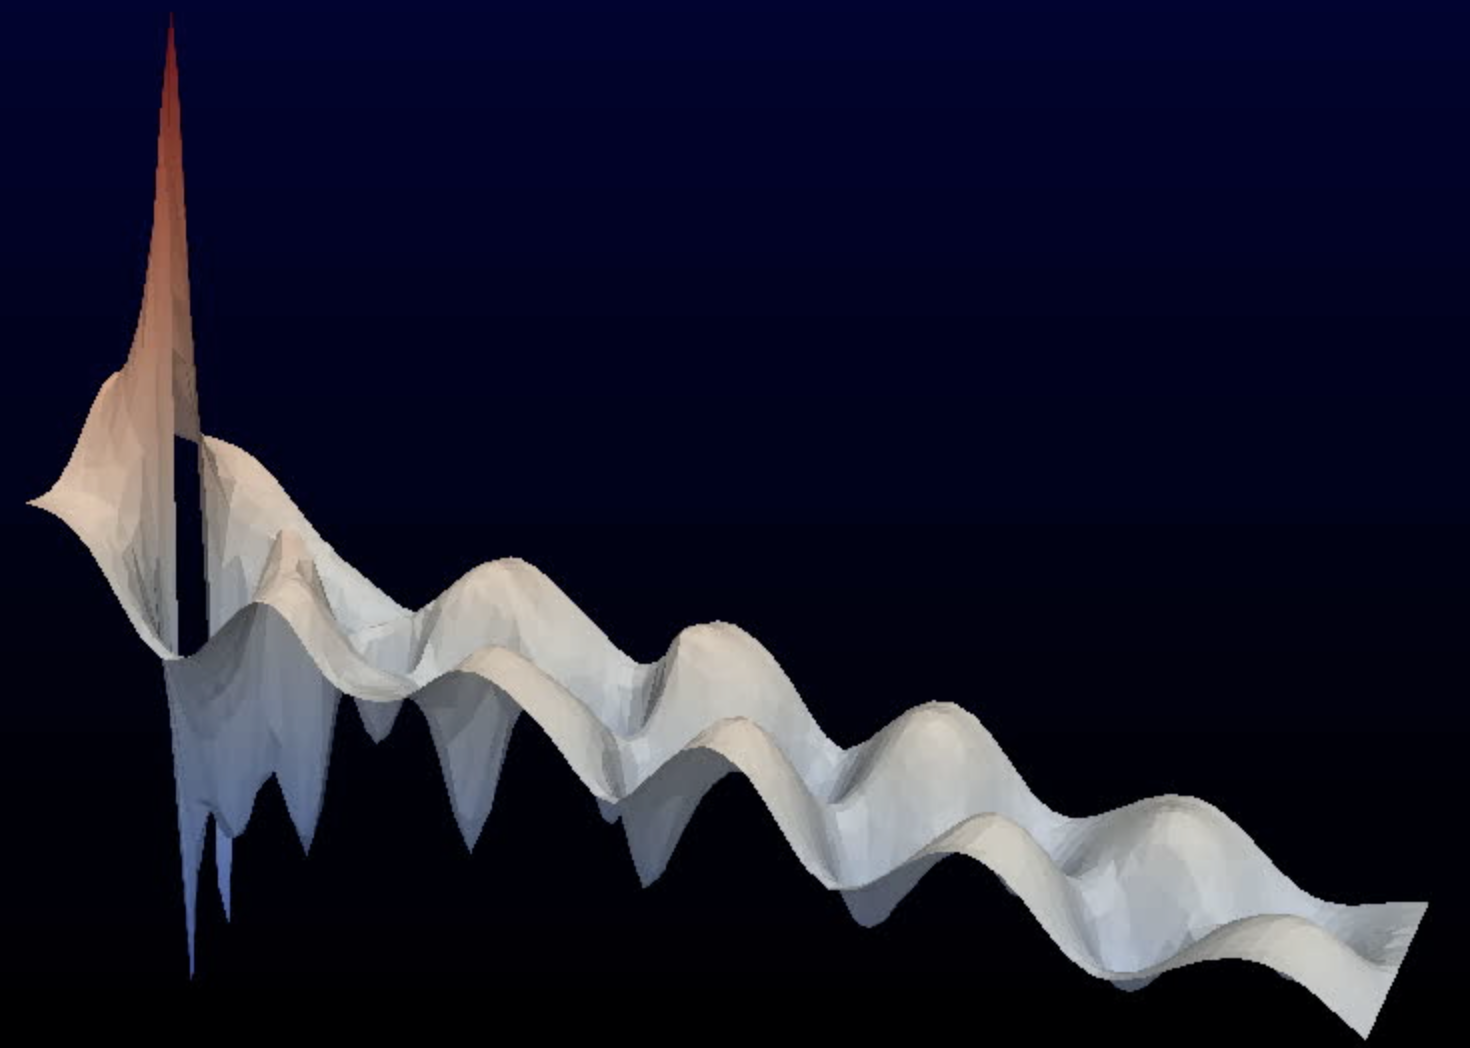
\includegraphics[width=0.95\linewidth]{fig/navier_stokes_cylinder_pressure.png}}
  \caption{
  Plot of the pressure for the cylinder test problem at final time. \label{ftut1:fig:navier_stokes_cylinder:pressure}
  }
\end{figure}
%\clearpage % flush figures ftut1:fig:navier_stokes_cylinder:pressure


The complete code for the cylinder test problem looks as
follows:

\begin{lstlisting}[language=Python,style=graycolor]
from fenics import *
from mshr import *
import numpy as np

T = 5.0            # final time
num_steps = 5000   # number of time steps
dt = T / num_steps # time step size
mu = 0.001         # dynamic viscosity
rho = 1            # density

# Create mesh
channel = Rectangle(Point(0, 0), Point(2.2, 0.41))
cylinder = Circle(Point(0.2, 0.2), 0.05)
domain = channel - cylinder
mesh = generate_mesh(domain, 64)

# Define function spaces
V = VectorFunctionSpace(mesh, 'P', 2)
Q = FunctionSpace(mesh, 'P', 1)

# Define boundaries
inflow   = 'near(x[0], 0)'
outflow  = 'near(x[0], 2.2)'
walls    = 'near(x[1], 0) || near(x[1], 0.41)'
cylinder = 'on_boundary && x[0]>0.1 && x[0]<0.3 && x[1]>0.1 && x[1]<0.3'

# Define inflow profile
inflow_profile = ('4.0*1.5*x[1]*(0.41 - x[1]) / pow(0.41, 2)', '0')

# Define boundary conditions
bcu_inflow = DirichletBC(V, Expression(inflow_profile, degree=2), inflow)
bcu_walls = DirichletBC(V, Constant((0, 0)), walls)
bcu_cylinder = DirichletBC(V, Constant((0, 0)), cylinder)
bcp_outflow = DirichletBC(Q, Constant(0), outflow)
bcu = [bcu_inflow, bcu_walls, bcu_cylinder]
bcp = [bcp_outflow]

# Define trial and test functions
u = TrialFunction(V)
v = TestFunction(V)
p = TrialFunction(Q)
q = TestFunction(Q)

# Define functions for solutions at previous and current time steps
u_n = Function(V)
u_  = Function(V)
p_n = Function(Q)
p_  = Function(Q)

# Define expressions used in variational forms
U  = 0.5*(u_n + u)
n  = FacetNormal(mesh)
f  = Constant((0, 0))
k  = Constant(dt)
mu = Constant(mu)
rho = Constant(rho)

# Define symmetric gradient
def epsilon(u):
    return sym(nabla_grad(u))

# Define stress tensor
def sigma(u, p):
    return 2*mu*epsilon(u) - p*Identity(len(u))

# Define variational problem for step 1
F1 = rho*dot((u - u_n) / k, v)*dx \
   + rho*dot(dot(u_n, nabla_grad(u_n)), v)*dx \
   + inner(sigma(U, p_n), epsilon(v))*dx \
   + dot(p_n*n, v)*ds - dot(mu*nabla_grad(U)*n, v)*ds \
   - dot(f, v)*dx
a1 = lhs(F1)
L1 = rhs(F1)

# Define variational problem for step 2
a2 = dot(nabla_grad(p), nabla_grad(q))*dx
L2 = dot(nabla_grad(p_n), nabla_grad(q))*dx - (1/k)*div(u_)*q*dx

# Define variational problem for step 3
a3 = dot(u, v)*dx
L3 = dot(u_, v)*dx - k*dot(nabla_grad(p_ - p_n), v)*dx

# Assemble matrices
A1 = assemble(a1)
A2 = assemble(a2)
A3 = assemble(a3)

# Apply boundary conditions to matrices
[bc.apply(A1) for bc in bcu]
[bc.apply(A2) for bc in bcp]

# Create XDMF files for visualization output
xdmffile_u = XDMFFile('navier_stokes_cylinder/velocity.xdmf')
xdmffile_p = XDMFFile('navier_stokes_cylinder/pressure.xdmf')

# Create time series (for use in reaction_system.py)
timeseries_u = TimeSeries('navier_stokes_cylinder/velocity_series')
timeseries_p = TimeSeries('navier_stokes_cylinder/pressure_series')

# Save mesh to file (for use in reaction_system.py)
File('navier_stokes_cylinder/cylinder.xml.gz') << mesh

# Create progress bar
progress = Progress('Time-stepping')
set_log_level(PROGRESS)

# Time-stepping
t = 0
for n in range(num_steps):

    # Update current time
    t += dt

    # Step 1: Tentative velocity step
    b1 = assemble(L1)
    [bc.apply(b1) for bc in bcu]
    solve(A1, u_.vector(), b1, 'bicgstab', 'hypre_amg')

    # Step 2: Pressure correction step
    b2 = assemble(L2)
    [bc.apply(b2) for bc in bcp]
    solve(A2, p_.vector(), b2, 'bicgstab', 'hypre_amg')

    # Step 3: Velocity correction step
    b3 = assemble(L3)
    solve(A3, u_.vector(), b3, 'cg', 'sor')

    # Plot solution
    plot(u_, title='Velocity')
    plot(p_, title='Pressure')

    # Save solution to file (XDMF/HDF5)
    xdmffile_u.write(u_, t)
    xdmffile_p.write(p_, t)

    # Save nodal values to file
    timeseries_u.store(u_.vector(), t)
    timeseries_p.store(p_.vector(), t)

    # Update previous solution
    u_n.assign(u_)
    p_n.assign(p_)

    # Update progress bar
    progress.update(t / T)
    print('u max:', u_.vector().array().max())

# Hold plot
interactive()
\end{lstlisting}
This program can be found in the file \href{{https://fenicsproject.org/pub/tutorial/python/vol1/ft08_navier_stokes_cylinder.py}}{\nolinkurl{ft08_navier_stokes_cylinder.py}}.
The reader should be advised that this example program is considerably
more demanding than our previous examples in terms of CPU time and
memory, but it should be possible to run the program on a reasonably
modern laptop.

\index{ft08\_navier\_stokes\_cylinder.py@{\rm\texttt{ft08\_navier\_stokes\_cylinder.py}}}


% !split
% Stand-alone notebook?

\section{A system of advection--diffusion--reaction equations}
\label{ftut1:reactionsystem}

\index{advection--diffusion--reaction}
\index{chemical reactions}
\index{reaction system}

The problems we have encountered so far---with the notable exception
of the Navier--Stokes equations---all share a common feature: they all
involve models expressed by a \emph{single} scalar or vector PDE. In many
situations the model is instead expressed as a system of PDEs,
describing different quantities possibly governed by (very) different
physics. As we saw for the Navier--Stokes equations, one way to solve
a system of PDEs in FEniCS is to use a splitting method where we solve
one equation at a time and feed the solution from one equation into
the next. However, one of the strengths with FEniCS is the ease by
which one can instead define variational problems that couple several
PDEs into one compound system. In this section, we will look at how to use
FEniCS to write solvers for such systems of coupled PDEs.
The goal is to demonstrate how easy it is to implement fully implicit,
also known as monolithic, solvers in FEniCS.

\index{coupled systems}

\subsection{PDE problem}

Our model problem is the following system of
advection--diffusion--reaction equations:

\begin{align}
  \label{ftut1:reactionsystem:system:1}
  \frac{\partial u_1}{\partial t} +
  w \cdot \nabla u_1 - \nabla\cdot(\epsilon\nabla u_1)
    &= f_1 -K u_1 u_2, \\
  \label{ftut1:reactionsystem:system:2}
  \frac{\partial u_2}{\partial t} +
  w \cdot \nabla u_2 - \nabla\cdot(\epsilon\nabla u_2)
    &= f_2 -K u_1 u_2, \\
  \label{ftut1:reactionsystem:system:3}
  \frac{\partial u_3}{\partial t} +
  w \cdot \nabla u_3 - \nabla\cdot(\epsilon\nabla u_3)
    &= f_3 + K u_1 u_2 - K u_3.
\end{align}

This system models the chemical reaction between two species $A$ and
$B$ in some domain $\Omega$:

\[
  A + B \rightarrow C.
\]

We assume that the reaction is \emph{first-order}, meaning that the
reaction rate is proportional to the concentrations $[A]$ and $[B]$ of
the two species $A$ and $B$:

\[
  \frac{\mathrm{d}}{\mathrm{d}t} [C] = K [A] [B].
\]
We also assume that the formed species $C$ spontaneously decays with a
rate proportional to the concentration $[C]$. In the PDE system
(\ref{ftut1:reactionsystem:system:1})--(\ref{ftut1:reactionsystem:system:3}),
we use the variables $u_1$, $u_2$, and $u_3$ to denote the
concentrations of the three species:

\[
  u_1 = [A], \quad u_2 = [B], \quad u_3 = [C].
\]
We see that the chemical reactions are accounted for in the
right-hand sides of the PDE system (\ref{ftut1:reactionsystem:system:1})--(\ref{ftut1:reactionsystem:system:3}).

The chemical reactions take part at each point in the domain
$\Omega$. In addition, we assume that the species $A$, $B$, and $C$
diffuse throughout the domain with diffusivity $\epsilon$ (the terms
$-\nabla\cdot(\epsilon\nabla u_i)$) and are advected with velocity
$w$ (the terms $w\cdot\nabla u_i$).

To make things visually and physically interesting, we shall let the
chemical reaction take place in the velocity field computed from the
solution of the incompressible Navier--Stokes equations around a
cylinder from the previous section. In summary, we will thus be
solving the following coupled system of nonlinear PDEs:

\begin{align}
  \label{ftut1:reactionsystem:full}
  \varrho\left(\frac{\partial w}{\partial t} +
  w \cdot \nabla w\right) &= \nabla\cdot\sigma(w, p) + f, \\
  \nabla \cdot w &= 0, \\
  \frac{\partial u_1}{\partial t} +
  w \cdot \nabla u_1 - \nabla\cdot(\epsilon\nabla u_1)
    &= f_1 - K u_1 u_2, \\
  \frac{\partial u_2}{\partial t} +
  w \cdot \nabla u_2 - \nabla\cdot(\epsilon\nabla u_2)
    &= f_2 - K u_1 u_2, \\
  \frac{\partial u_3}{\partial t} +
  w \cdot \nabla u_3 - \nabla\cdot(\epsilon\nabla u_3)
    &= f_3 + K u_1 u_2 - K u_3.
\end{align}
We assume that $u_1 = u_2 = u_3 = 0$ at $t = 0$ and inject the species
$A$ and $B$ into the system by specifying nonzero source terms $f_1$
and $f_2$ close to the corners at the inflow, and take $f_3 = 0$. The
result will be that $A$ and $B$ are convected by advection and
diffusion throughout the channel, and when they mix the species $C$
will be formed.

Since the system is one-way coupled from the Navier--Stokes subsystem
to the advection--diffusion--reaction subsystem, we do not need to
recompute the solution to the Navier--Stokes equations, but can just
read back the previously computed velocity field $w$ and feed it into
our equations. But we \emph{do} need to learn how to read and write
solutions for time-dependent PDE problems.

\subsection{Variational formulation}

We obtain the variational formulation of our system by multiplying
each equation by a test function, integrating the second-order terms
$-\nabla\cdot(\epsilon\nabla u_i)$ by parts, and summing up the
equations. When working with FEniCS it is convenient to think of the
PDE system as a vector of equations. The test functions are collected in
a vector too, and the variational formulation is the inner product of
the vector PDE and the vector test function.

We also need introduce some discretization in time. We will use the
backward Euler method as before when we solved the heat equation and
approximate the time derivatives by $(u_i^{n+1}-u_i^n) / \dt$. Let
$v_1$, $v_2$, and $v_3$ be the test functions, or the components of
the test vector function. The inner product results in

\begin{align}
  \label{ftut1:reactionsystem:varproblem}
  & \int_{\Omega}
  (\dt^{-1} (u_1^{n+1} - u_1^n) v_1 + w \cdot \nabla u^{n+1}_1 \, v_1
  + \epsilon \nabla u^{n+1}_1 \cdot \nabla v_1) \dx \\
  + & \int_{\Omega} (\dt^{-1} (u_2^{n+1} - u_2^n) v_2
  + w \cdot \nabla u^{n+1}_2 \, v_2
  + \epsilon \nabla u^{n+1}_2 \cdot \nabla v_2) \dx \nonumber \\
  + & \int_{\Omega} (\dt^{-1} (u_3^{n+1} - u_3^n) v_3
  + w \cdot \nabla u^{n+1}_3 \, v_3
  + \epsilon \nabla u^{n+1}_3 \cdot \nabla v_3) \dx \nonumber \\
  - & \int_{\Omega} (f_1 v_1 + f_2 v_2 + f_3 v_3) \dx \nonumber \\
  - & \int_{\Omega} (-K u^{n+1}_1 u^{n+1}_2 v_1 - K u^{n+1}_1
  u^{n+1}_2 v_2 + K u^{n+1}_1 u^{n+1}_2 v_3 - K u^{n+1}_3 v_3) \dx = 0.
  \nonumber
\end{align}
For this problem it is natural to assume homogeneous Neumann boundary
conditions on the entire boundary for $u_1$, $u_2$, and $u_3$; that
is, $\partial u_i/\partial n = 0$ for $i = 1, 2, 3$. This means that
the boundary terms vanish when we integrate by parts.

\subsection{FEniCS implementation}

The first step is to read the mesh from file. Luckily, we made sure to
save the mesh to file in the Navier--Stokes example and can now easily
read it back from file:

\begin{lstlisting}[language=Python,style=graycolor]
mesh = Mesh('navier_stokes_cylinder/cylinder.xml.gz')
\end{lstlisting}
The mesh is stored in the native FEniCS XML format (with additional
gzipping to decrease the file size).

Next, we need to define the finite element function space. For this
problem, we need to define several spaces. The first space we create
is the space for the velocity field $w$ from the Navier--Stokes
simulation. We call this space $W$ and define the space by

\begin{lstlisting}[language=Python,style=graycolor]
W = VectorFunctionSpace(mesh, 'P', 2)
\end{lstlisting}
It is important that this space is exactly the same as the space we
used for the velocity field in the Navier--Stokes solver. To read the
values for the velocity field, we use a \texttt{TimeSeries}:

\index{TimeSeries@{\rm\texttt{TimeSeries}}}

\begin{lstlisting}[language=Python,style=graycolor]
timeseries_w = TimeSeries('navier_stokes_cylinder/velocity_series')
\end{lstlisting}
This will initialize the object \Verb!timeseries_w! which we will call
later in the time-stepping loop to retrieve values from the
file \Verb!velocity_series.h5! (in binary HDF5 format).

\index{mixed function space}
\index{mixed finite element}
\index{MixedElement@{\rm\texttt{MixedElement}}}

For the three concentrations $u_1$, $u_2$, and $u_3$, we want to
create a \emph{mixed space} with functions that represent the full system
$(u_1, u_2, u_3)$ as a single entity. To do this, we need to define a
\texttt{MixedElement} as the product space of three simple finite elements
and then used the mixed element to define the function space:

\begin{lstlisting}[language=Python,style=graycolor]
P1 = FiniteElement('P', triangle, 1)
element = MixedElement([P1, P1, P1])
V = FunctionSpace(mesh, element)
\end{lstlisting}


\begin{warning_mdfboxadmon}[Mixed elements as products of elements]
FEniCS also allows finite elements to be defined as products of simple
elements (or mixed elements). For example, the well-known Taylor--Hood
element, with quadratic velocity components and linear pressure functions,
may be defined as follows:

\begin{lstlisting}[language=Python,style=graycolor]
P2 = VectorElement('P', triangle, 2)
P1 = FiniteElement('P', triangle, 1)
TH = P2 * P1
\end{lstlisting}
This syntax works great for two elements, but for three or more
elements we meet a subtle issue in how the Python interpreter handles
the \texttt{*} operator. For the reaction system, we create the mixed element
by \texttt{element = MixedElement([P1, P1, P1])} and one would be tempted to
write

\begin{lstlisting}[language=Python,style=graycolor]
element = P1 * P1 * P1
\end{lstlisting}
However, this is equivalent to writing \texttt{element = (P1 * P1) * P1} so
the result will be a mixed element consisting of two subsystems, the
first of which in turn consists of two scalar subsystems.

Finally, we remark that for the simple case of a mixed system
consisting of three scalar elements as for the reaction system, the
definition is in fact equivalent to using a standard vector-valued
element:

\index{VectorElement@{\rm\texttt{VectorElement}}}

\begin{lstlisting}[language=Python,style=graycolor]
element = VectorElement('P', triangle, 1, dim=3)
V = FunctionSpace(mesh, element)
\end{lstlisting}
\end{warning_mdfboxadmon} % title: Mixed elements as products of elements


Once the space has been created, we need to define our test functions
and finite element functions. Test functions for a mixed function
space can be created by replacing \texttt{TestFunction} by \texttt{TestFunctions}:

\begin{lstlisting}[language=Python,style=graycolor]
v_1, v_2, v_3 = TestFunctions(V)
\end{lstlisting}

Since the problem is nonlinear, we need to work with functions rather
than trial functions for the unknowns. This can be done by using the
corresponding \texttt{Functions} construction in FEniCS. However, as we will
need to access the \texttt{Function} for the entire system itself, we first
need to create that function and then access its components:

\begin{lstlisting}[language=Python,style=graycolor]
u = Function(V)
u_1, u_2, u_3 = split(u)
\end{lstlisting}
These functions will be used to represent the unknowns $u_1$, $u_2$, and $u_3$
at the new time level $n+1$. The corresponding values at the previous
time level $n$ are denoted by \Verb!u_n1!, \Verb!u_n2!, and \Verb!u_n3! in our program.

When now all functions and test functions have been defined, we can
express the nonlinear variational problem
(\ref{ftut1:reactionsystem:varproblem}):

\begin{lstlisting}[language=Python,style=graycolor]
F = ((u_1 - u_n1) / k)*v_1*dx + dot(w, grad(u_1))*v_1*dx \
  + eps*dot(grad(u_1), grad(v_1))*dx + K*u_1*u_2*v_1*dx  \
  + ((u_2 - u_n2) / k)*v_2*dx + dot(w, grad(u_2))*v_2*dx \
  + eps*dot(grad(u_2), grad(v_2))*dx + K*u_1*u_2*v_2*dx  \
  + ((u_3 - u_n3) / k)*v_3*dx + dot(w, grad(u_3))*v_3*dx \
  + eps*dot(grad(u_3), grad(v_3))*dx - K*u_1*u_2*v_3*dx + K*u_3*v_3*dx \
  - f_1*v_1*dx - f_2*v_2*dx - f_3*v_3*dx
\end{lstlisting}

The time-stepping simply consists of solving this variational problem
in each time step by a call to the \texttt{solve} function:

\begin{lstlisting}[language=Python,style=graycolor]
t = 0
for n in range(num_steps):
    t += dt
    timeseries_w.retrieve(w.vector(), t)
    solve(F == 0, u)
    u_n.assign(u)
\end{lstlisting}
In each time step, we first read the current value for the velocity
field from the time series we have previously stored. We then solve
the nonlinear system, and assign the computed values to the left-hand
side values for the next time interval. When retrieving values from a
\texttt{TimeSeries}, the values will by default be interpolated (linearly) to
the given time \texttt{t} if the time does not exactly match a sample in the
series.

The solution at the final time is shown in Figure~\ref{ftut1:fig:reactionsystem:solution}. We
clearly see the advection of the species $A$ and $B$ and the formation
of $C$ along the center of the channel where $A$ and $B$ meet.


\begin{figure}[!ht]  % ftut1:fig:reactionsystem:solution
  \centerline{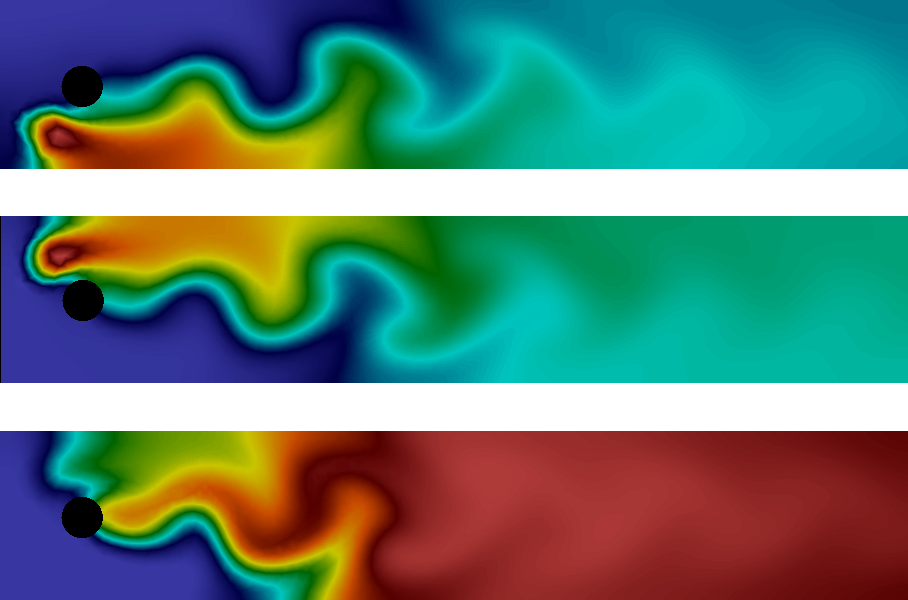
\includegraphics[width=0.95\linewidth]{fig/reaction_system.png}}
  \caption{
  Plot of the concentrations of the three species $A$, $B$, and $C$ (from top to bottom) at final time. \label{ftut1:fig:reactionsystem:solution}
  }
\end{figure}
%\clearpage % flush figures ftut1:fig:reactionsystem:solution

The complete code is presented below.

\begin{lstlisting}[language=Python,style=graycolor]
from fenics import *

T = 5.0            # final time
num_steps = 500    # number of time steps
dt = T / num_steps # time step size
eps = 0.01         # diffusion coefficient
K = 10.0           # reaction rate

# Read mesh from file
mesh = Mesh('navier_stokes_cylinder/cylinder.xml.gz')

# Define function space for velocity
W = VectorFunctionSpace(mesh, 'P', 2)

# Define function space for system of concentrations
P1 = FiniteElement('P', triangle, 1)
element = MixedElement([P1, P1, P1])
V = FunctionSpace(mesh, element)

# Define test functions
v_1, v_2, v_3 = TestFunctions(V)

# Define functions for velocity and concentrations
w = Function(W)
u = Function(V)
u_n = Function(V)

# Split system functions to access components
u_1, u_2, u_3 = split(u)
u_n1, u_n2, u_n3 = split(u_n)

# Define source terms
f_1 = Expression('pow(x[0]-0.1,2)+pow(x[1]-0.1,2)<0.05*0.05 ? 0.1 : 0',
                 degree=1)
f_2 = Expression('pow(x[0]-0.1,2)+pow(x[1]-0.3,2)<0.05*0.05 ? 0.1 : 0',
                 degree=1)
f_3 = Constant(0)

# Define expressions used in variational forms
k = Constant(dt)
K = Constant(K)
eps = Constant(eps)

# Define variational problem
F = ((u_1 - u_n1) / k)*v_1*dx + dot(w, grad(u_1))*v_1*dx \
  + eps*dot(grad(u_1), grad(v_1))*dx + K*u_1*u_2*v_1*dx  \
  + ((u_2 - u_n2) / k)*v_2*dx + dot(w, grad(u_2))*v_2*dx \
  + eps*dot(grad(u_2), grad(v_2))*dx + K*u_1*u_2*v_2*dx  \
  + ((u_3 - u_n3) / k)*v_3*dx + dot(w, grad(u_3))*v_3*dx \
  + eps*dot(grad(u_3), grad(v_3))*dx - K*u_1*u_2*v_3*dx + K*u_3*v_3*dx \
  - f_1*v_1*dx - f_2*v_2*dx - f_3*v_3*dx

# Create time series for reading velocity data
timeseries_w = TimeSeries('navier_stokes_cylinder/velocity_series')

# Create VTK files for visualization output
vtkfile_u_1 = File('reaction_system/u_1.pvd')
vtkfile_u_2 = File('reaction_system/u_2.pvd')
vtkfile_u_3 = File('reaction_system/u_3.pvd')

# Create progress bar
progress = Progress('Time-stepping')
set_log_level(PROGRESS)

# Time-stepping
t = 0
for n in range(num_steps):

    # Update current time
    t += dt

    # Read velocity from file
    timeseries_w.retrieve(w.vector(), t)

    # Solve variational problem for time step
    solve(F == 0, u)

    # Save solution to file (VTK)
    _u_1, _u_2, _u_3 = u.split()
    vtkfile_u_1 << (_u_1, t)
    vtkfile_u_2 << (_u_2, t)
    vtkfile_u_3 << (_u_3, t)

    # Update previous solution
    u_n.assign(u)

    # Update progress bar
    progress.update(t / T)

# Hold plot
interactive()
\end{lstlisting}
This example program can be found in the file \href{{https://fenicsproject.org/pub/tutorial/python/vol1/ft09_reaction_system.py}}{\nolinkurl{ft09_reaction_system.py}}.

\index{ft09\_reaction\_system.py@{\rm\texttt{ft09\_reaction\_system.py}}}

Finally, we comment on three important techniques that are very useful
when working with systems of PDEs: setting initial conditions, setting
boundary conditions, and extracting components of the system for
plotting or postprocessing.

\paragraph{Setting initial conditions for mixed systems.}
\index{initial condition}

In our example, we did not need to worry about setting an initial
condition, since we start with $u_1 = u_2 = u_3 = 0$. This happens
automatically in the code when we set \Verb!u_n = Function(V)!. This
creates a \texttt{Function} for the whole system and all degrees of freedom
are set to zero.

If we want to set initial conditions for the components of the system
separately, the easiest solution is to define the initial conditions
as a vector-valued \texttt{Expression} and then project (or interpolate) this
to the \texttt{Function} representing the whole system. For example,

\begin{lstlisting}[language=Python,style=graycolor]
u_0 = Expression(('sin(x[0])', 'cos(x[0]*x[1])', 'exp(x[1])'), degree=1)
u_n = project(u_0, V)
\end{lstlisting}
This defines $u_1$, $u_2$, and $u_2$ to be the projections of $\sin
x$, $\cos (xy)$, and $\exp(y)$, respectively.

\paragraph{Setting boundary conditions for mixed systems.}
In our example, we also did not need to worry about setting boundary
conditions since we used a natural Neumann condition. If we want to set
Dirichlet conditions for individual components of the system, this can
be done as usual by the class \texttt{DirichletBC}, but we must specify for
which subsystem we set the boundary condition. For example, to specify
that $u_2$ should be equal to $xy$ on the boundary defined by
\texttt{boundary}, we do

\begin{lstlisting}[language=Python,style=graycolor]
u_D = Expression('x[0]*x[1]', degree=1)
bc = DirichletBC(V.sub(1), u_D, boundary)
\end{lstlisting}
The object \texttt{bc} or a list of such objects containing different
boundary conditions, can then be passed to the \texttt{solve} function as usual.
Note that numbering starts at $0$ in FEniCS so the subspace
corresponding to $u_2$ is \texttt{V.sub(1)}.

\paragraph{Accessing components of mixed systems.}
\index{components}
\index{split@{\rm\texttt{split}}}

If \texttt{u} is a \texttt{Function} defined on a mixed function space in FEniCS,
there are several ways in which \texttt{u} can be \emph{split} into components.
Above we already saw an example of the first of these:

\begin{lstlisting}[language=Python,style=graycolor]
u_1, u_2, u_3 = split(u)
\end{lstlisting}
This extracts the components of \texttt{u} as \emph{symbols} that can be used in a
variational problem. The above statement is in fact equivalent to

\begin{lstlisting}[language=Python,style=graycolor]
u_1 = u[0]
u_2 = u[1]
u_3 = u[2]
\end{lstlisting}
Note that \texttt{u[0]} is not really a \texttt{Function} object, but merely a
symbolic expression, just like \texttt{grad(u)} in FEniCS is a symbolic
expression and not a \texttt{Function} representing the gradient.  This means
that \Verb!u_1!, \Verb!u_2!, \Verb!u_3! can be used in a variational problem, but
cannot be used for plotting or postprocessing.

To access the components of \texttt{u} for plotting and saving the solution
to file, we need to use a different variant of the \texttt{split} function:

\begin{lstlisting}[language=Python,style=graycolor]
u_1_, u_2_, u_3_ = u.split()
\end{lstlisting}
This returns three subfunctions as actual objects with access to the
common underlying data stored in \texttt{u}, which makes plotting and saving
to file possible. Alternatively, we can do

\index{deep copy}

\begin{lstlisting}[language=Python,style=graycolor]
u_1_, u_2_, u_3_ = u.split(deepcopy=True)
\end{lstlisting}
which will create \Verb!u_1_!, \Verb!u_2_!, and \Verb!u_3_! as stand-alone \texttt{Function}
objects, each holding a copy of the subfunction data extracted from
\texttt{u}. This is useful in many situations but is not necessary for
plotting and saving solutions to file.

% !split
\chapter{Subdomains and boundary conditions}
\label{ch:subdomains}

\index{subdomains}


\begin{quote}
So far, we have only looked briefly at how to specify boundary
conditions. In this chapter, we look more closely at how to specify
boundary conditions on specific parts (subdomains) of the boundary and
how to combine multiple boundary conditions. We will also look at how to
generate meshes with subdomains and how to define coefficients
with different values in different subdomains.
\end{quote}


% ========= Multiple domains and boundaries =========

\section{Combining Dirichlet and Neumann conditions}
\label{ch:poisson0:DN}

Let's return to the Poisson problem from Chapter~\ref{ch:fundamentals}
and see how to extend the mathematics and the implementation to handle
a Dirichlet condition in combination with a Neumann condition. The
domain is still the unit square, but now we set the Dirichlet
condition $u=\ub$ at the left and right sides, $x=0$ and $x=1$, while
the Neumann condition

\begin{equation*}
-{\partial u\over\partial n}=g
\end{equation*}
is applied to the remaining
sides $y=0$ and $y=1$.

% The Neumann condition is also known as a \emph{natural boundary condition}
% (in contrast to an essential boundary condition).

\index{Neumann boundary condition}

\subsection{PDE problem}

Let $\GD$ and $\GN$ denote the parts of the boundary $\partial\Omega$
where the Dirichlet and Neumann conditions apply, respectively. The
complete boundary-value problem can be written as

\begin{alignat}{2}
    - \nabla^2 u &= f \quad&&\mbox{in } \Omega,  \\
    u &= \ub &&\mbox{on } \GD,       \\
    - {\partial u\over\partial n} &= g &&\mbox{on } \GN  \tp
\end{alignat}
Again, we choose $u=1+x^2 + 2y^2$ as the exact solution and adjust $f$, $g$, and
$\ub$ accordingly:

\begin{align*}
f(x, y) &= -6,\\
g(x, y) &= \left\lbrace\begin{array}{ll}
0, & \quad y=0,\\
4, & \quad y=1,
\end{array}\right.\\
\ub(x, y) &= 1 + x^2 + 2y^2\tp
\end{align*}

For ease of programming, we define $g$ as a function over the whole
domain $\Omega$ such that $g$ takes on the correct values at $y=0$ and
$y=1$. One possible extension is

\begin{equation*}
g(x,y) = 4y\tp
\end{equation*}

\subsection{Variational formulation}

The first task is to derive the variational formulation. This time we cannot
omit the boundary term arising from the integration by parts, because
$v$ is only zero on $\GD$. We have

\begin{equation*}
 -\int_\Omega (\nabla^2 u)v \dx
= \int_\Omega\nabla u\cdot\nabla v \dx - \int_{\partial\Omega}{\partial u\over
\partial n}v \ds,
\end{equation*}
and since $v=0$ on $\GD$,

\begin{equation*}
- \int_{\partial\Omega}{\partial u\over
\partial n}v \ds
=
- \int_{\GN}{\partial u\over
\partial n}v \ds
= \int_{\GN}gv \ds,
\end{equation*}
by applying the boundary condition on $\GN$.
The resulting weak form reads

\begin{equation}
\int_{\Omega} \nabla u \cdot \nabla v \dx
= \int_{\Omega} fv \dx - \int_{\GN} gv \ds\tp
\label{ch:poisson0:2D:DN:weak}
\end{equation}
Expressing this equation
in the standard notation $a(u,v)=L(v)$ is straightforward with

\begin{align}
a(u, v) &= \int_{\Omega} \nabla u \cdot \nabla v \dx,
\label{ftut:poisson2:vard:a}\\
L(v) &= \int_{\Omega} fv \dx -
\int_{\GN} gv \ds\tp  \label{ftut:poisson2:vard:L}
\end{align}

\subsection{FEniCS implementation}

How does the Neumann condition impact the implementation?  Let us
revisit our previous implementation
\href{{https://fenicsproject.org/pub/tutorial/python/vol1/ft01_poisson.py}}{\nolinkurl{ft01_poisson.py}}
from Section~\ref{ch:poisson0:impl} and examine which changes
we need to make to incorporate the Neumann condition. It turns out
that only two changes are necessary:

\begin{itemize}
  \item The function \texttt{boundary} defining the Dirichlet boundary
    must be modified.

  \item The new boundary term must be added to the expression for \texttt{L}.
\end{itemize}

\noindent
The first adjustment can be coded as

\begin{lstlisting}[language=Python,style=graycolor]
tol = 1E-14

def boundary_D(x, on_boundary):
    if on_boundary:
        if near(x[0], 0, tol) or near(x[0], 1, tol):
            return True
        else:
            return False
    else:
        return False
\end{lstlisting}
A more compact implementation reads

\begin{lstlisting}[language=Python,style=graycolor]
def boundary_D(x, on_boundary):
    return on_boundary and (near(x[0], 0, tol) or near(x[0], 1, tol))
\end{lstlisting}

\index{near@{\rm\texttt{near}}}

The second adjustment of our program concerns the definition of \texttt{L},
which needs to include the Neumann condition:

\begin{lstlisting}[language=Python,style=graycolor]
g = Expression('4*x[1]', degree=1)
L = f*v*dx - g*v*ds
\end{lstlisting}
The \texttt{ds} variable implies a boundary integral, while \texttt{dx}
implies an integral over the domain $\Omega$.
No other modifications are necessary.

Note that the integration \texttt{*ds} is carried out over the entire
boundary, including the Dirichlet boundary. However, since the test
function \texttt{v} vanishes on the Dirichlet boundary (as a result
specifying a \texttt{DirichletBC}), the integral will only include the
contribution from the Neumann boundary.

% !split
\section{Setting multiple Dirichlet conditions}
\label{ch:poisson0:multiple:Dirichlet}

In the previous section, we used a single function $\ub(x,y)$ for
setting Dirichlet conditions on two parts of the boundary. Often it
is more practical to use multiple functions, one for each subdomain of the
boundary. Let us return to the case from Section~\ref{ch:poisson0:DN}
and redefine the problem in terms of two Dirichlet conditions:

\begin{alignat*}{2}
    - \nabla^2 u &= f \quad&&\mbox{in } \Omega, \\
    u &= u_{_\mathrm{L}} &&\mbox{on } \GD^{^{\mathrm{L}}}, \\
    u &= u_{_\mathrm{R}} &&\mbox{on } \GD^{^{\mathrm{R}}}, \\
    - {\partial u\over\partial n} &= g &&\mbox{on } \GN \tp
\end{alignat*}
Here, $\GD^{^{\mathrm{L}}}$ is the left boundary $x=0$, while
$\GD^{^{\mathrm{R}}}$ is the right boundary $x=1$. We note that
$u_{_\mathrm{L}}(x, y) = 1 + 2y^2$,
$u_{_\mathrm{R}}(x, y) = 2 + 2y^2$, and
$g(x, y)=4y$.

For the boundary condition on $\GD^{^{\mathrm{L}}}$, we define the
usual triple of an expression for the boundary value, a function
defining the location of the boundary, and a \texttt{DirichletBC} object:

\begin{lstlisting}[language=Python,style=graycolor]
u_L = Expression('1 + 2*x[1]*x[1]', degree=2)

def boundary_L(x, on_boundary):
    tol = 1E-14
    return on_boundary and near(x[0], 0, tol)

bc_L = DirichletBC(V, u_L, boundary_L)
\end{lstlisting}
For the boundary condition on $\GD^{^{\mathrm{R}}}$, we write a
similar code snippet:

\begin{lstlisting}[language=Python,style=graycolor]
u_R = Expression('2 + 2*x[1]*x[1]', degree=2)

def boundary_R(x, on_boundary):
    tol = 1E-14
    return on_boundary and near(x[0], 1, tol)

bc_R = DirichletBC(V, u_R, boundary_R)
\end{lstlisting}
We collect the two boundary conditions in a list which
we can pass to the \texttt{solve} function to compute the solution:

\begin{lstlisting}[language=Python,style=graycolor]
bcs = [bc_L, bc_R]
...
solve(a == L, u, bcs)
\end{lstlisting}

Note that for boundary values that do not depend on $x$ or $y$, we
might replace the \texttt{Expression} objects by \texttt{Constant} objects.

% !split
\section{Defining subdomains for different materials}
\label{ftut:possion:2D:2mat:impl}

\index{heterogeneous media}
\index{multi-material domain}

Solving PDEs in domains made up of different materials is a frequently
encountered task. In FEniCS, these kinds of problems are handled by
defining subdomains inside the domain. A simple example with two
materials (subdomains) in 2D will demonstrate the idea. We consider
the following variable-coefficient extension of the Poisson equation
from Chapter~\ref{ch:fundamentals}:

\begin{equation} \label{ch:poisson0:2D:2mat:varcoeff2}
  -\nabla \cdot \left\lbrack \kappa(x,y)\nabla u(x,y)\right\rbrack =
  f(x, y),
\end{equation}
in some domain $\Omega$.
Physically, this problem may be viewed as a model of heat conduction,
with variable heat conductivity $\kappa(x, y) \geq
\underline{\kappa} > 0$.

For illustration purposes, we consider the domain $\Omega =
[0,1]\times [0,1]$ and divide it into two equal subdomains, as
depicted in Figure~\ref{fig:subdomains}:

\begin{equation*}
\Omega_0 = [0, 1]\times [0,1/2],\quad
\Omega_1 = [0, 1]\times (1/2,1]\tp
\end{equation*}
We define $\kappa(x,y)=\kappa_0$ in $\Omega_0$ and $\kappa(x,y)=\kappa_1$ in $\Omega_1$,
where $\kappa_0, \kappa_1 > 0$ are given constants.


\begin{figure}[!ht]  % fig:subdomains
  \centerline{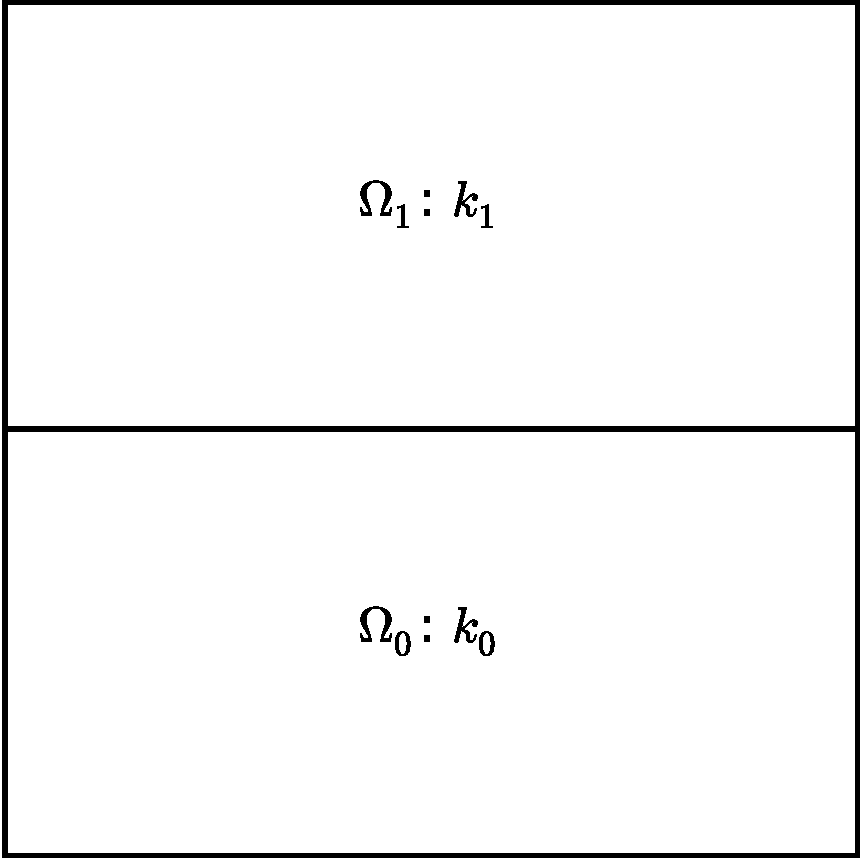
\includegraphics[width=0.5\linewidth]{fig/subdomains.pdf}}
  \caption{
  Two subdomains with different material parameters. \label{fig:subdomains}
  }
\end{figure}
%\clearpage % flush figures fig:subdomains


The variational formulation may be easily expressed in FEniCS as
follows:
\begin{lstlisting}[language=Python,style=graycolor]
a = kappa*dot(grad(u), grad(v))*dx
L = f*v*dx
\end{lstlisting}
In the remainder of this section, we will discuss different strategies
for defining the coefficient \texttt{kappa} as an \texttt{Expression} that takes on
different values in the two subdomains.

\subsection{Using expressions to define subdomains}

The simplest way to implement a variable coefficient $\kappa =
\kappa(x, y)$ is to define an \texttt{Expression} which depends on the
coordinates $x$ and $y$. We have previously used the \texttt{Expression}
class to define expressions based on simple formulas. Aternatively,
an \texttt{Expression} can be defined as a Python class which allows for more
complex logic. The following code snippet illustrates this
construction:

\begin{lstlisting}[language=Python,style=graycolor]
class K(Expression):
    def set_k_values(self, k_0, k_1):
        self.k_0, self.k_1 = k_0, k_1

    def eval(self, value, x):
        "Set value[0] to value at point x"
        tol = 1E-14
        if x[1] <= 0.5 + tol:
            value[0] = self.k_0
        else:
            value[0] = self.k_1

# Initialize kappa
kappa = K(degree=0)
kappa.set_k_values(1, 0.01)
\end{lstlisting}
The \texttt{eval} method gives great flexibility in defining functions, but a
downside is that FEniCS will call \texttt{eval} in Python for each node \texttt{x},
which is a slow process.

An alternative method is to use a C++ string expression as we have
seen before, which is much more efficient in FEniCS. This can be done
using an inline if test:

\begin{lstlisting}[language=Python,style=graycolor]
tol = 1E-14
k_0 = 1.0
k_1 = 0.01
kappa = Expression('x[1] <= 0.5 + tol ? k_0 : k_1', degree=0,
               tol=tol, k_0=k_0, k_1=k_1)
\end{lstlisting}

This method of defining variable coefficients works if the subdomains
are simple shapes that can be expressed in terms of geometric
inequalities. However, for more complex subdomains, we will need to
use a more general technique, as we will see next.

\index{boundary specification (class)}

\subsection{Using mesh functions to define subdomains}

\index{boundary markers}
\index{MeshFunction@{\rm\texttt{MeshFunction}}}
\index{CellFunction@{\rm\texttt{CellFunction}}}
\index{FacetFunction@{\rm\texttt{FacetFunction}}}

We now address how to specify the subdomains $\Omega_0$ and $\Omega_1$
using a more general technique. This technique involves the use of two
classes that are essential in FEniCS when working with subdomains:
\texttt{SubDomain} and \texttt{MeshFunction}. Consider the following definition of the
boundary $x = 0$:

\begin{lstlisting}[language=Python,style=graycolor]
def boundary(x, on_boundary):
    tol = 1E-14
    return on_boundary and near(x[0], 0, tol)
\end{lstlisting}
This boundary definition is actually a shortcut to the more general
FEniCS concept \texttt{SubDomain}. A \texttt{SubDomain} is a class which defines a
region in space (a subdomain) in terms of a member function \texttt{inside}
which returns \texttt{True} for points that belong to the subdomain and
\texttt{False} for points that don't belong to the subdomain. Here is how to
specify the boundary $x = 0$ as a \texttt{SubDomain}:

\begin{lstlisting}[language=Python,style=graycolor]
class Boundary(SubDomain):
    def inside(self, x, on_boundary):
        tol = 1E-14
        return on_boundary and near(x[0], 0, tol)

boundary = Boundary()
bc = DirichletBC(V, Constant(0), boundary)
\end{lstlisting}
We notice that the \texttt{inside} function of the class \texttt{Boundary} is
(almost) identical to the previous boundary definition in terms of the
\texttt{boundary} function. Technically, our class \texttt{Boundary} is a
\emph{subclass} of the FEniCS class \texttt{SubDomain}.

% A word about computer science terminology may be in order here: The term
% \emph{instance} means a Python object of a particular type (such as
% \texttt{SubDomain}, \texttt{Function}, \texttt{FunctionSpace}, etc.).  Many use \emph{instance}
% and \emph{object} as interchangeable terms. In other computer programming
% languages one may also use the term \emph{variable} for the same thing. We
% mostly use the well-known term \emph{object} in this text.

We will use two \texttt{SubDomain} subclasses to define the two subdomains
$\Omega_0$ and $\Omega_1$:

\begin{lstlisting}[language=Python,style=graycolor]
tol = 1E-14

class Omega_0(SubDomain):
    def inside(self, x, on_boundary):
        return x[1] <= 0.5 + tol

class Omega_1(SubDomain):
    def inside(self, x, on_boundary):
        return x[1] >= 0.5 - tol
\end{lstlisting}
Notice the use of \texttt{<=} and \texttt{>=} in both tests. FEniCS will call the
\texttt{inside} function for each vertex in a cell to determine whether or
not the cell belongs to a particular subdomain. For this reason, it is
important that the test holds for all vertices in cells aligned with
the boundary. In addition, we use a tolerance to make sure that
vertices on the internal boundary at $y = 0.5$ will belong to \emph{both}
subdomains. This is a little counter-intuitive, but is necessary to
make the cells both above and below the internal boundary belong to
either $\Omega_0$ or $\Omega_1$.

To define the variable coefficient $\kappa$, we will use a powerful tool in
FEniCS called a \texttt{MeshFunction}. A \texttt{MeshFunction} is a discrete
function that can be evaluated at a set of so-called \emph{mesh
entities}. A mesh entity in FEniCS is either a vertex, an edge, a
face, or a cell (triangle or tetrahedron). A \texttt{MeshFunction} over cells
is suitable to represent subdomains (materials), while a
\texttt{MeshFunction} over facets (edges or faces) is used to represent
pieces of external or internal boundaries. A \texttt{MeshFunction} over cells
can also be used to represent boundary markers for mesh refinement. A
FEniCS \texttt{MeshFunction} is parameterized both over its data type (like
integers or booleans) and its dimension (0 = vertex, 1 = edge
etc.). Special subclasses \texttt{VertexFunction}, \texttt{EdgeFunction} etc. are
provided for easy definition of a \texttt{MeshFunction} of a particular
dimension.

Since we need to define subdomains of $\Omega$ in the present example,
we make use of a \texttt{CellFunction}. The constructor
is given two arguments: (1) the type of value: \texttt{'int'} for integers,
\Verb!'size_t'! for non-negative (unsigned) integers, \texttt{'double'} for real
numbers, and \texttt{'bool'} for logical values; (2) a \texttt{Mesh} object.
Alternatively, the constructor can take just a filename and initialize
the \texttt{CellFunction} from data in a file.

We first create a \texttt{CellFunction} with non-negative
integer values (\Verb!'size_t'!):

\begin{lstlisting}[language=Python,style=graycolor]
materials = CellFunction('size_t', mesh)
\end{lstlisting}

Next, we use the two subdomains to \emph{mark} the cells belonging to each
subdomain:
\begin{lstlisting}[language=Python,style=graycolor]
subdomain_0 = Omega_0()
subdomain_1 = Omega_1()
subdomain_0.mark(materials, 0)
subdomain_1.mark(materials, 1)
\end{lstlisting}

This will set the values of the mesh function \texttt{materials} to $0$ on
each cell belonging to $\Omega_0$ and $1$ on all cells belonging to
$\Omega_1$. Alternatively, we can use the following equivalent code to
mark the cells:

\begin{lstlisting}[language=Python,style=graycolor]
materials.set_all(0)
subdomain_1.mark(materials, 1)
\end{lstlisting}
To examine the values of the mesh function and see that we have indeed
defined our subdomains correctly, we can simply plot the mesh
function:

\begin{lstlisting}[language=Python,style=graycolor]
plot(materials, interactive=True)
\end{lstlisting}
We may also wish to store the values of the mesh function for later
use:
\begin{lstlisting}[language=Python,style=graycolor]
File('materials.xml.gz') << materials
\end{lstlisting}
which can later be read back from file as follows:
\begin{lstlisting}[language=Python,style=graycolor]
File('materials.xml.gz') >> materials
\end{lstlisting}

Now, to use the values of the mesh function \texttt{materials} to define the
variable coefficient $\kappa$, we create a FEniCS \texttt{Expression}:

\begin{lstlisting}[language=Python,style=graycolor]
class K(Expression):
    def __init__(self, materials, k_0, k_1, **kwargs):
        self.materials = materials
        self.k_0 = k_0
        self.k_1 = k_1

def eval_cell(self, values, x, cell):
        if self.materials[cell.index] == 0:
            values[0] = self.k_0
        else:
            values[0] = self.k_1

kappa = K(materials, k_0, k_1, degree=0)
\end{lstlisting}

This is similar to the \texttt{Expression} subclass we defined above, but we
make use of the member function \Verb!eval_cell! in place of the regular
\texttt{eval} function. This version of the evaluation function has an
additional \texttt{cell} argument which we can use to check on which cell we
are currently evaluating the function.  We also defined the special
function \Verb!__init__! (the constructor) so that we can pass all data to
the \texttt{Expression} when it is created.

Since we make use of geometric tests to define the two \texttt{SubDomains}
for $\Omega_0$ and $\Omega_1$, the \texttt{MeshFunction} method may seem like
an unnecessary complication of the simple method using an
\texttt{Expression} with an if-test. However, in general the definition of
subdomains may be available as a \texttt{MeshFunction} (from a data file),
perhaps generated as part of the mesh generation process, and not as a
simple geometric test. In such cases the method demonstrated here is
the recommended way to work with subdomains.

\index{CompiledSubDomain@{\rm\texttt{CompiledSubDomain}}}

% May not work if the dofs are renumbered
% ===== Vectorized version of subdomain definitions =====
%
% To speed up this code, we can vectorize the expressions:
%
% !bc pycod
% materials = CellFunction('size_t', mesh)
% materials.set_all(0)  # "the rest"
% for m, subdomain in enumerate(subdomains[1:], 1):
% subdomain.mark(materials, m)
%
% kappa_values = kappa
% V0 = FunctionSpace(mesh, 'DG', 0)
% kappa = Function(V0)
% help = np.asarray(materials.array(), dtype=np.int32)
% kappa.vector()[:] = np.choose(help, kappa_values)
% !ec
% The \texttt{help} array is required since \texttt{choose} cannot work with
% \texttt{materials.array()} because this array has elements of
% type \texttt{uint32}. We must therefore transform this array to an array
% \texttt{help} with standard \texttt{int32} integers.

\subsection{Using C++ code snippets to define subdomains}

The \texttt{SubDomain} and \texttt{Expression} Python classes are very convenient,
but their use leads to function calls from C++ to Python for each node
in the mesh. Since this involves a significant cost, we need to make
use of C++ code if performance is an issue.

Instead of writing the \texttt{SubDomain} subclass in Python, we may instead use
the \texttt{CompiledSubDomain} tool in FEniCS to specify the subdomain in C++
code and thereby speed up our code. Consider
the definition of the classes \Verb!Omega_0! and \Verb!Omega_1! above in Python. The
key strings that define these subdomains can be expressed in C++ syntax
and given as arguments to \texttt{CompiledSubDomain} as follows:

\begin{lstlisting}[language=Python,style=graycolor]
tol = 1E-14
subdomain_0 = CompiledSubDomain('x[1] <= 0.5 + tol', tol=tol)
subdomain_1 = CompiledSubDomain('x[1] >= 0.5 - tol', tol=tol)
\end{lstlisting}
As seen, parameters can be specified using keyword arguments.
The resulting objects, \Verb!subdomain_0! and \Verb!subdomain_1!, can be used
as ordinary \texttt{SubDomain} objects.

Compiled subdomain strings can be applied for specifying boundaries as
well:

\begin{lstlisting}[language=Python,style=graycolor]
boundary_R = CompiledSubDomain('on_boundary && near(x[0], 1, tol)',
                               tol=1E-14)
\end{lstlisting}

It is also possible to feed the C++ string (without parameters)
directly as the third argument to \texttt{DirichletBC} without explicitly
constructing a \texttt{CompiledSubDomain} object:

\begin{lstlisting}[language=Python,style=graycolor]
bc1 = DirichletBC(V, value, 'on_boundary && near(x[0], 1, tol)')
\end{lstlisting}

Python \texttt{Expression} classes may also be redefined using C++ for more
efficient code. Consider again the definition of the class \texttt{K} above
for the variable coefficient $\kappa = \kappa(x)$. This may be redefined using a
C++ code snippet and the keyword \texttt{cppcode} to the regular FEniCS
\texttt{Expression} class:

\begin{lstlisting}[language=Python,style=graycolor]
cppcode = """
class K : public Expression
{
public:

  void eval(Array<double>& values,
            const Array<double>& x,
            const ufc::cell& cell) const
  {
    if ((*materials)[cell.index] == 0)
      values[0] = k_0;
    else
      values[0] = k_1;
  }

  std::shared_ptr<MeshFunction<std::size_t>> materials;
  double k_0;
  double k_1;

};
"""

kappa = Expression(cppcode=cppcode, degree=0)
kappa.materials = materials
kappa.k_0 = k_0
kappa.k_1 = k_1
\end{lstlisting}

% !split
\section{Setting multiple Dirichlet, Neumann, and Robin conditions}
\label{ch:poisson0:multi:bc}
\index{Dirichlet boundary condition}
\index{Neumann boundary condition}
\index{Robin boundary condition}
\index{boundary conditions}

Consider again the variable-coefficient Poisson problem
from Section~\ref{ftut:possion:2D:2mat:impl}. We will now discuss
how to implement general combinations of boundary conditions of
Dirichlet, Neumann, and Robin type for this model problem.

\subsection{Three types of boundary conditions}

We extend our repertoire of boundary conditions to three types:
Dirichlet, Neumann, and Robin. Dirichlet conditions apply to some
parts $\GD^0, \GD^1, \ldots$, of the boundary:

\[ u = \ub^0\hbox{ on }\GD^0,\quad
   u = \ub^1\hbox{ on }\GD^1, \quad \ldots,\]
where $\ub^i$ are prescribed functions, $i=0,1,\ldots$.
On other parts, $\GN^0, \GN^1, \ldots$, we have
Neumann conditions:

\[ -\kappa{\partial u\over\partial n} = g_{0}\hbox{ on }\GN^0,\quad
-\kappa{\partial u\over\partial n} = g_{1}\hbox{ on }\GN^1,\quad \ldots,
\]
Finally, we have \emph{Robin conditions}:

\begin{equation*}
-\kappa{\partial u\over\partial n} = r(u-s),
\label{ch:poisson0:multi:bc:Robin}
\end{equation*}
where $r$ and $s$ are specified functions.  The Robin condition is
most often used to model heat transfer to the surroundings and arise
naturally from Newton's cooling law. In that case, $r$ is a heat
transfer coefficient, and $s$ is the temperature of the
surroundings. Both can be space and time-dependent.
The Robin conditions apply
at some parts $\GR^0, \GR^1, \ldots$, of the boundary:

\[ -\kappa{\partial u\over\partial n} = r_0(u-s_0)\hbox{ on }\GR^0,\quad
-\kappa{\partial u\over\partial n} = r_1(u-s_1)\hbox{ on }\GR^1,\quad \ldots
\]

\subsection{PDE problem}

With the notation above, the model problem to be solved with multiple
Dirichlet, Neumann, and Robin conditions can be formulated as follows:

\begin{alignat}{2}
-\nabla\cdot(\kappa\nabla u) &= f \quad&&\mbox{in } \Omega, \label{ch:poisson0:2D:DN3}\\
u &= \ub^i &&\mbox{on } \GD^i,\quad i=0,1,\ldots
\label{ch:poisson0:2D:DN3:bcD}\\
-\kappa{\partial u\over\partial n} &= g_i &&\mbox{on } \GN^i,\quad
i=0,1,\ldots
\label{ch:poisson0:2D:DN3:bcN}\\
-\kappa{\partial u\over\partial n} &= r_i(u-s_i) \quad&&\mbox{on } \GR^i,\quad
i=0,1,\ldots
\label{ch:poisson0:2D:DN3:bcR}
\end{alignat}

\subsection{Variational formulation}

As usual, we multiply by a test function $v$ and integrate by parts:

\begin{equation*}
 -\int_\Omega \nabla\cdot(\kappa\nabla u) v \dx
= \int_\Omega \kappa\nabla u\cdot \nabla v \dx -
\int_{\partial\Omega}\kappa\frac{\partial u}{\partial n}v \ds\tp
\end{equation*}
On the Dirichlet part of the boundary ($\GD^i$), the boundary integral
vanishes since $v = 0$. On the remaining part of the boundary, we
split the boundary integral into contributions from the Neumann parts
($\GN^i$) and Robin parts ($\GR^i$). Inserting the boundary conditions,
we obtain

\begin{align*}
-\int_{\partial\Omega} \kappa\frac{\partial u}{\partial n}v \ds
&=
-\sum_i\int_{\GN^i} \kappa\frac{\partial u}{\partial n} \ds
-\sum_i\int_{\GR^i} \kappa\frac{\partial u}{\partial n} \ds\\
&=
\sum_i\int_{\GN^i}g_i \ds +
\sum_i\int_{\GR^i}r_i(u-s_i) \ds\tp
\end{align*}
We thus obtain the following variational problem:

\begin{equation}
F = \int_{\Omega} \kappa\nabla u\cdot \nabla v \dx +
\sum_i\int_{\GN^i} g_iv \ds +
\sum_i\int_{\GR^i}r_i(u-s_i)v \ds
- \int_{\Omega} fv \dx =0\tp
\label{ch:poisson0:multi:bc:varform}
\end{equation}

We have been used to writing this variational formulation in the
standard notation $a(u,v)=L(v)$, which requires that we identify all
integral depending on the trial function $u$, and collect these in
$a(u,v)$, while the remaining integrals go into $L(v)$. The integrals
from the Robin condition must for this reason be split into two parts:

\begin{equation*}
\int_{\GR^i}r_i(u-s_i)v \ds
= \int_{\GR^i} r_iuv \ds - \int_{\GR^i}r_is_iv \ds\tp
\end{equation*}
We then have

\begin{align}
a(u, v) &= \int_{\Omega} \kappa\nabla u\cdot \nabla v \dx
+ \sum_i\int_{\GR^i}r_iuv \ds,
\label{ch:poisson0:2D:DN3:var:a}\\
L(v) &= \int_{\Omega} fv \dx -
\sum_i\int_{\GN^i} g_i v \ds + \sum_i\int_{\GR^i}r_is_iv \ds\tp
\label{ch:poisson0:2D:DN3:var:L}
\end{align}
Alternatively, we may keep the formulation
(\ref{ch:poisson0:multi:bc:varform}) and either solve the variational
problem as a nonlinear problem (\texttt{F == 0}) in FEniCS or use the FEniCS
functions \texttt{lhs} and \texttt{rhs} to extract the bilinear and linear parts of
\texttt{F}:

\begin{lstlisting}[language=Python,style=graycolor]
a = lhs(F)
L = rhs(F)
\end{lstlisting}
Note that if we choose to solve this linear problem as a nonlinear
problem, the Newton iteration will converge in a single iteration.

\subsection{FEniCS implementation}

Let us examine how to extend our Poisson solver to handle general
combinations of Dirichlet, Neumann, and Robin boundary conditions.
Compared to our previous code, we must consider the following
extensions:

\begin{itemize}
  \item Defining markers for the different parts of the boundary.

  \item Splitting the boundary integral into parts using the markers.
\end{itemize}

\noindent
A general approach to the first task is to mark each of the desired
boundary parts with markers 0, 1, 2, and so forth. Here we aim at the
four sides of the unit square, marked with 0 ($x=0$), 1 ($x=1$), 2
($y=0$), and 3 ($y=1$).  The markers will be defined using a
\texttt{MeshFunction}, but contrary to Section~\ref{ftut:possion:2D:2mat:impl}, this is not a function over cells, but
a function over the facets of the mesh. We use a \texttt{FacetFunction} for
this purpose:

\begin{lstlisting}[language=Python,style=graycolor]
boundary_markers = FacetFunction('size_t', mesh)
\end{lstlisting}
As in Section~\ref{ftut:possion:2D:2mat:impl} we use a subclass of
\texttt{SubDomain} to identify the various parts of the mesh
function. Problems with domains of more complicated geometries may set
the mesh function for marking boundaries as part of the mesh
generation.  In our case, the boundary $x = 0$ can be marked
as follows:

\begin{lstlisting}[language=Python,style=graycolor]
class BoundaryX0(SubDomain):
    tol = 1E-14
    def inside(self, x, on_boundary):
        return on_boundary and near(x[0], 0, tol)

bx0 = BoundaryX0()
bx0.mark(boundary_markers, 0)
\end{lstlisting}
Similarly, we create the classes \texttt{BoundaryX1} ($x=1$), \texttt{BoundaryY0}
($y=0$), and \texttt{BoundaryY1} ($y=1$) boundary, and mark these as
subdomains 1, 2, and 3, respectively.

For generality of the implementation, we let the user specify
what kind of boundary condition that applies to each of the four
boundaries. We set up a Python dictionary for this purpose, with
the key as subdomain number and the value as a dictionary specifying
the kind of condition as key and a function as its value.
For example,

\begin{lstlisting}[language=Python,style=graycolor]
boundary_conditions = {0: {'Dirichlet': u_D},
                       1: {'Robin':     (r, s)},
                       2: {'Neumann':   g},
                       3: {'Neumann',   0}}
\end{lstlisting}
specifies

\begin{itemize}
 \item a Dirichlet condition $u = \ub$ for $x = 0$;

 \item a Robin condition $-\kappa\partial_n u = r(u-s)$ for $x = 1$;

 \item a Neumann condition $-\kappa\partial_n u = g$ for $y = 0$;

 \item a Neumann condition $-\kappa\partial_n u = 0$ for $y = 1$.
\end{itemize}

\noindent
As explained in Section~\ref{ch:poisson0:multiple:Dirichlet}, multiple
Dirichlet conditions must be collected in a list of \texttt{DirichletBC}
objects. Based on the \Verb!boundary_conditions! data structure above, we
can construct this list by the following code snippet:

\begin{lstlisting}[language=Python,style=graycolor]
bcs = []
for i in boundary_conditions:
    if 'Dirichlet' in boundary_conditions[i]:
        bc = DirichletBC(V, boundary_conditions[i]['Dirichlet'],
                         boundary_markers, i)
        bcs.append(bc)
\end{lstlisting}

A new aspect of the variational problem is the two distinct
boundary integrals over $\GN^i$ and $\GR^i$.
Having a mesh function over exterior cell facets (our
\Verb!boundary_markers! object), where subdomains (boundary parts) are
numbered as $0,1,2,\ldots$, the special symbol \texttt{ds(0)}
implies integration over subdomain (part) 0, \texttt{ds(1)} denotes
integration over subdomain (part) 1, and so on.
The idea of multiple \texttt{ds}-type objects generalizes to volume
integrals too: \texttt{dx(0)}, \texttt{dx(1)}, etc., are used to
integrate over subdomain 0, 1, etc.,  inside $\Omega$.

To express integrals over the boundary parts using \texttt{ds(i)}, we must
first redefine the measure \texttt{ds} in terms of our boundary markers:

\begin{lstlisting}[language=Python,style=graycolor]
ds = Measure('ds', domain=mesh, subdomain_data=boundary_markers)
\end{lstlisting}
Similarly, if we want integration over different parts of the domain,
we redefine \texttt{dx} as

\begin{lstlisting}[language=Python,style=graycolor]
dx = Measure('dx', domain=mesh, subdomain_data=domain_markers)
\end{lstlisting}
where \Verb!domain_markers! is a \texttt{CellFunction} defining subdomains in $\Omega$.

Suppose we have a Robin condition with values \texttt{r} and \texttt{s} on subdomain
\texttt{R}, and a Neumann condition with value \texttt{g} on subdomain \texttt{N}. The
variational form can then be written

\begin{lstlisting}[language=Python,style=graycolor]
a = kappa*dot(grad(u), grad(v))*dx + r*u*v*ds(R)
L = f*v*dx - g*v*ds(N) + r*s*v*ds(R)
\end{lstlisting}

In our case, things get a bit more complicated since the
information about integrals in Neumann and Robin conditions
are in the \Verb!boundary_conditions! data structure. We can collect
all Neumann conditions by the following code snippet:

\begin{lstlisting}[language=Python,style=graycolor]
integrals_N = []
for i in boundary_conditions:
    if 'Neumann' in boundary_conditions[i]:
        if boundary_conditions[i]['Neumann'] != 0:
            g = boundary_conditions[i]['Neumann']
            integrals_N.append(g*v*ds(i))
\end{lstlisting}
Applying \Verb!sum(integrals_N)! will apply the \texttt{+} operator to
the variational forms in the \Verb!integrals_N! list and result
in the integrals we need for the right-hand side \texttt{L} of the
variational form.

The integrals in the Robin condition can similarly be collected
in lists:

\begin{lstlisting}[language=Python,style=graycolor]
integrals_R_a = []
integrals_R_L = []
for i in boundary_conditions:
    if 'Robin' in boundary_conditions[i]:
        r, s = boundary_conditions[i]['Robin']
        integrals_R_a.append(r*u*v*ds(i))
        integrals_R_L.append(r*s*v*ds(i))
\end{lstlisting}

We are now in a position to define the \texttt{a} and \texttt{L} expressions
in the variational formulation:

\begin{lstlisting}[language=Python,style=graycolor]
a = kappa*dot(grad(u), grad(v))*dx + sum(integrals_R_a)
L = f*v*dx - sum(integrals_N) + sum(integrals_R_L)
\end{lstlisting}

\index{lhs@{\rm\texttt{lhs}}}
\index{rhs@{\rm\texttt{rhs}}}

Alternatively, we may use the FEniCS functions \texttt{lhs} and \texttt{rhs} as
mentioned above to simplify the extraction of terms for the Robin
integrals:

\begin{lstlisting}[language=Python,style=graycolor]
integrals_R = []
for i in boundary_conditions:
    if 'Robin' in boundary_conditions[i]:
        r, s = boundary_conditions[i]['Robin']
        integrals_R.append(r*(u - s)*v*ds(i))

F = kappa*dot(grad(u), grad(v))*dx + \
    sum(integrals_R) - f*v*dx + sum(integrals_N)
a, L = lhs(F), rhs(F)
\end{lstlisting}
This time we can more naturally define the integrals from the
Robin condition as \texttt{r*(u - s)*v*ds(i)}.

The complete code can be found in the function
\Verb!solver_bcs! in the program
\href{{https://fenicsproject.org/pub/tutorial/python/vol1/ft10_poisson_extended.py}}{\nolinkurl{ft10_poisson_extended.py}}.

\index{ft10\_poisson\_extended.py@{\rm\texttt{ft10\_poisson\_extended.py}}}

\subsection{Test problem}

We will use the same exact solution $\uex=1+x^2+2y^2$ as in Chapter~\ref{ch:fundamentals}, and thus take $\kappa=1$ and $f=-6$. Our domain
is the unit square, and we assign Dirichlet conditions at $x=0$ and
$x=1$, a Robin condition at $y=0$, and a Neumann condition at
$y=1$. With the given exact solution $\uex$, we realize that the
Neumann condition at $y=1$ is $-\partial u / \partial n = - \partial u /
\partial y = 4y = 4$, while the Robin condition at $y=0$ can be selected in
many ways. Since $-\partial u/\partial n=\partial u/\partial y=0$ at
$y=0$, we can select $s=\uex$ and specify $r \neq 0$ arbitrarily in the
Robin condition. We will set $r = 1000$ and $s = \uex$.

The boundary parts are thus $\GD^0$: $x=0$, $\GD^1$: $x=1$,
$\GR^0$: $y=0$, and $\GN^0$: $y=1$.

When implementing this test problem, and especially other test
problems with more complicated expressions, it is advantageous to use
symbolic computing. Below we define the exact solution as a \texttt{sympy}
expression and derive other functions from their mathematical
definitions.  Then we turn these expressions into C/C++ code, which
can then be used to define \texttt{Expression} objects.

\begin{lstlisting}[language=Python,style=graycolor]
# Define manufactured solution in sympy and derive f, g, etc.
import sympy as sym
x, y = sym.symbols('x[0], x[1]')            # needed by UFL
u = 1 + x**2 + 2*y**2                       # exact solution
u_e = u                                     # exact solution
u_00 = u.subs(x, 0)                         # restrict to x = 0
u_01 = u.subs(x, 1)                         # restrict to x = 1
f = -sym.diff(u, x, 2) - sym.diff(u, y, 2)  # -Laplace(u)
f = sym.simplify(f)                         # simplify f
g = -sym.diff(u, y).subs(y, 1)              # compute g = -du/dn
r = 1000                                    # Robin data, arbitrary
s = u                                       # Robin data, u = s

# Collect variables
variables = [u_e, u_00, u_01, f, g, r, s]

# Turn into C/C++ code strings
variables = [sym.printing.ccode(var) for var in variables]

# Turn into FEniCS Expressions
variables = [Expression(var, degree=2) for var in variables]

# Extract variables
u_e, u_00, u_01, f, g, r, s = variables

# Define boundary conditions
boundary_conditions = {0: {'Dirichlet': u_00},   # x = 0
                       1: {'Dirichlet': u_01},   # x = 1
                       2: {'Robin':     (r, s)}, # y = 0
                       3: {'Neumann':   g}}      # y = 1
\end{lstlisting}

The complete code can be found in the function
\Verb!demo_bcs! in the program
\href{{https://fenicsproject.org/pub/tutorial/python/vol1/ft10_poisson_extended.py}}{\nolinkurl{ft10_poisson_extended.py}}.

\subsection{Debugging boundary conditions}

It is easy to make mistakes when implementing a problem with many
different types of boundary conditions, as in the present case. One
method to debug boundary conditions is to run through all vertex
coordinates and check if the \texttt{SubDomain.inside} method marks the
vertex as on the boundary. Another useful method is to list which
degrees of freedom that are subject to Dirichlet conditions, and for
first-order Lagrange ($\mathsf{P}_1$) elements, print the
corresponding vertex coordinates as illustrated by the following
code snippet:

\begin{lstlisting}[language=Python,style=graycolor]
if debug1:

    # Print all vertices that belong to the boundary parts
    for x in mesh.coordinates():
        if bx0.inside(x, True): print('%s is on x = 0' % x)
        if bx1.inside(x, True): print('%s is on x = 1' % x)
        if by0.inside(x, True): print('%s is on y = 0' % x)
        if by1.inside(x, True): print('%s is on y = 1' % x)

    # Print the Dirichlet conditions
    print('Number of Dirichlet conditions:', len(bcs))
    if V.ufl_element().degree() == 1:  # P1 elements
        d2v = dof_to_vertex_map(V)
        coor = mesh.coordinates()
        for i, bc in enumerate(bcs):
            print('Dirichlet condition %d' % i)
            boundary_values = bc.get_boundary_values()
            for dof in boundary_values:
                print('   dof %2d: u = %g' % (dof, boundary_values[dof]))
                if V.ufl_element().degree() == 1:
                    print('    at point %s' %
                          (str(tuple(coor[d2v[dof]].tolist()))))
\end{lstlisting}


\begin{notice_mdfboxadmon}[Calls to the \texttt{inside} method]
In the code snippet above, we call the inside method for each
coordinate of the mesh. We could also place a printout inside the
\texttt{inside} method. Then it will be surprising to see that this method is
called not only for the points assoicated with degrees of freedom.
For $\mathsf{P}_1$ elements the method is also called for each
midpoint on each facet of the cells. This is because a Dirichlet
condition is by default set only if the entire facet can be said to be
subject to the condition defining the boundary.
\end{notice_mdfboxadmon} % title: Calls to the \texttt{inside} method



% !split
\section{Generating meshes with subdomains}

So far, we have worked mostly with simple meshes (the unit square) and
defined boundaries and subdomains in terms of simple geometric tests
like $x = 0$ or $y \leq 0.5$. For more complex geometries, it is not
realistic to specify boundaries and subdomains in this way. Instead,
the boundaries and subdomains must be defined as part of the mesh
generation process. We will now look at how to use the FEniCS mesh
generation tool \texttt{mshr} to generate meshes and define subdomains.

\subsection{PDE problem}

\index{magnetostatics}
\index{Maxwell's equations}

We will again solve the Poisson equation, but this time for a
different application. Consider an iron cylinder with copper wires
wound around the cylinder as in Figure~\ref{ftut1:fig:magnetostatics:geometry}. Through the copper wires a
static current $J = 1\,\mathrm{A}$ is flowing and we want to compute
the magnetic field $B$ in the iron cylinder, the copper wires, and the
surrounding vacuum.


\begin{figure}[!ht]  % ftut1:fig:magnetostatics:geometry
  \centerline{
\includegraphics[width=0.5\linewidth]{fig/magnetostatics_geometry.pdf}}
  \caption{
  Cross-section of an iron cylinder with copper wires wound around the cylinder, here with $n = 8$ windings. The inner circles are cross-sections of the copper wire coming up (`\protect `north'') and the outer circles are cross-sections of the copper wire going down into the plane (``south''). \label{ftut1:fig:magnetostatics:geometry}
  }
\end{figure}
%\clearpage % flush figures ftut1:fig:magnetostatics:geometry


First, we simplify the problem to a 2D problem. We can do this by
assuming that the cylinder extends far along the $z$-axis and as a
consequence the field is virtually independent of the
$z$-coordinate. Next, we consider Maxwell's equation to derive a
Poisson equation for the magnetic field (or rather its potential):

\begin{align}
  \nabla\cdot  D &= \varrho, \\
  \nabla\cdot  B &= 0, \\
  \nabla\times E &= -\frac{\partial B}{\partial t}, \\
  \nabla\times H &= \frac{\partial D}{\partial t} + J.
\end{align}
Here, $D$ is the displacement field, $B$ is the magnetic
field, $E$ is the electric field, and $H$ is the magnetizing field. In
addition to Maxwell's equations, we also need a constitutive relation
between $B$ and $H$,

\begin{equation}
  B = \mu H,
\end{equation}
which holds for an isotropic linear magnetic medium. Here, $\mu$ is the
magnetic permeability of the material. Now, since $B$ is solenoidal
(divergence free) according to Maxwell's equations, we know that $B$
must be the curl of some vector field $A$. This field is called the
magnetic vector potential. Since the problem is static and thus
$\partial D/\partial t = 0$, it follows that

\begin{equation}
  J = \nabla \times H
    = \nabla \times (\mu^{-1} B)
    = \nabla \times (\mu^{-1} \nabla \times A)
    = -\nabla \cdot (\mu^{-1} \nabla A).
\end{equation}
In the last step, we have expanded the second derivatives and used the
gauge freedom of $A$ to simplify the equations to a simple
vector-valued Poisson problem for the magnetic vector potential; if $B
= \nabla \times A$, then $B = \nabla \times (A + \nabla \psi)$ for any
scalar field $\psi$ (the gauge function). For the current problem, we
thus need to solve the following 2D Poisson problem for the
$z$-component $A_z$ of the magnetic vector potential:

\begin{align}
  - \nabla \cdot (\mu^{-1} \nabla A_z) &= J_z \quad \text{in } \Real^2, \\
  \lim_{|(x, y)| \rightarrow \infty} A_z &= 0.
\end{align}
Since we cannot solve this problem on an infinite domain, we will
truncate the domain using a large disk and set $A_z = 0$ on the
boundary. The current $J_z$ is set to $+1\,\mathrm{A}$ in the interior
set of circles (copper wire cross-sections) and to $-1\,\mathrm{A}$ in
the exterior set of circles in Figure~\ref{ftut1:fig:magnetostatics:geometry}.

\index{infinite domain}

Once the magnetic vector potential has been computed, we can
compute the magnetic field $B = B(x, y)$ by

\begin{align}
  B(x, y) =
  \left(\frac{\partial A_z}{\partial y},
       -\frac{\partial A_z}{\partial x}\right).
\end{align}

\subsection{Variational formulation}

The variational problem is derived as before by multiplying the PDE
with a test function $v$ and integrating by parts. Since the boundary
integral vanishes due to the Dirichlet condition, we obtain

\begin{equation}
  \int_{\Omega} \mu^{-1} \nabla A_z \cdot \nabla v \dx
  = \int_{\Omega} J_z v \dx,
\end{equation}
or, in other words, $a(A_z, v) = L(v)$ with

\begin{align}
  a(A_z, v) &= \int_{\Omega} \mu^{-1} \nabla A_z \cdot \nabla v \dx, \\
  L(v) &= \int_{\Omega} J_z v \dx.
\end{align}

\subsection{FEniCS implementation}

The first step is to generate a mesh for the geometry described in
Figure~\ref{ftut1:fig:magnetostatics:geometry}. We let $a$ and $b$ be the
inner and outer radii of the iron cylinder and let $c_1$ and $c_2$
be the radii of the two concentric distributions of copper wire
cross-sections. Furthermore, we let $r$ be the radius of a copper
wire, $R$ be the radius of our domain, and $n$ be the number of
windings (giving a total of $2n$ copper-wire cross-sections). This
geometry can be described easily using \texttt{mshr} and a little bit of
Python programming:

\index{mshr}
\index{Circle@{\rm\texttt{Circle}}}
\index{generate\_mesh@{\rm\texttt{generate\_mesh}}}
\index{mesh generation}

\begin{lstlisting}[language=Python,style=graycolor]
# Define geometry for background
domain = Circle(Point(0, 0), R)

# Define geometry for iron cylinder
cylinder = Circle(Point(0, 0), b) - Circle(Point(0, 0), a)

# Define geometry for wires (N = North (up), S = South (down))
angles_N = [i*2*pi/n for i in range(n)]
angles_S = [(i + 0.5)*2*pi/n for i in range(n)]
wires_N = [Circle(Point(c_1*cos(v), c_1*sin(v)), r) for v in angles_N]
wires_S = [Circle(Point(c_2*cos(v), c_2*sin(v)), r) for v in angles_S]
\end{lstlisting}

The mesh that we generate will be a mesh of the entire disk with
radius $R$ but we need the mesh generation to respect the internal
boundaries defined by the iron cylinder and the copper wires. We also
want \texttt{mshr} to label the subdomains so that we can easily specify
material parameters ($\mu$) and currents. To do this, we use the
\texttt{mshr} function \Verb!set_subdomain! as follows:

\begin{lstlisting}[language=Python,style=graycolor]
# Set subdomain for iron cylinder
domain.set_subdomain(1, cylinder)

# Set subdomains for wires
for (i, wire) in enumerate(wires_N):
    domain.set_subdomain(2 + i, wire)
for (i, wire) in enumerate(wires_S):
    domain.set_subdomain(2 + n + i, wire)
\end{lstlisting}
Once the subdomains have been created, we can generate the mesh:

\begin{lstlisting}[language=Python,style=graycolor]
mesh = generate_mesh(domain, 32)
\end{lstlisting}
A detail of the mesh is shown in Figure~\ref{ftut1:fig:magnetostatics:mesh}.


\begin{figure}[!ht]  % ftut1:fig:magnetostatics:mesh
  \centerline{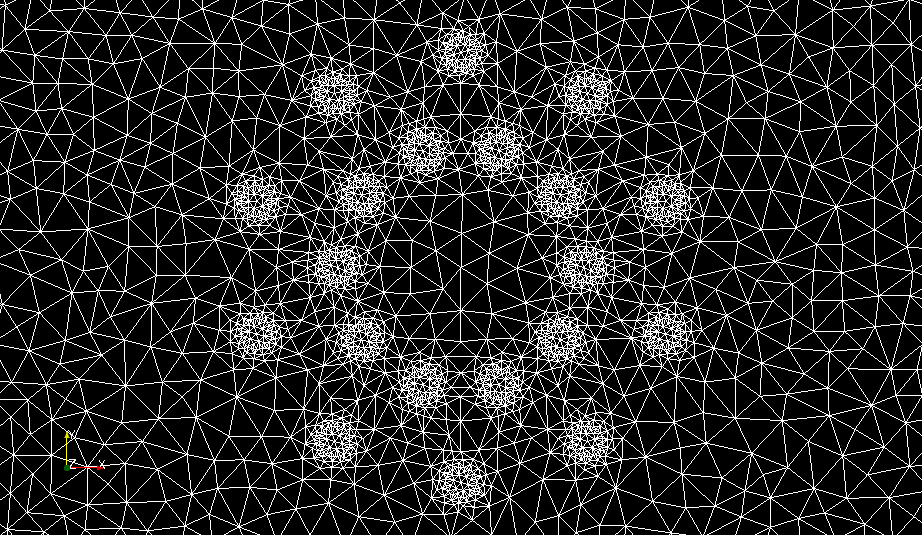
\includegraphics[width=0.95\linewidth]{fig/magnetostatics_mesh.png}}
  \caption{
  Plot of (part of) the mesh generated for the magnetostatics test problem. The subdomains for the iron cylinder and copper wires are clearly visible \label{ftut1:fig:magnetostatics:mesh}
  }
\end{figure}
%\clearpage % flush figures ftut1:fig:magnetostatics:mesh

The mesh generated with \texttt{mshr} will contain information about the
subdomains we have defined. To use this information in the definition of
our variational problem and subdomain-dependent parameters, we will need to
create a \texttt{MeshFunction} that marks the subdomains. This can be easily
created by a call to the member function \texttt{mesh.domains}, which holds
the subdomain data generated by \texttt{mshr}:

\begin{lstlisting}[language=Python,style=graycolor]
markers = MeshFunction('size_t', mesh, 2, mesh.domains())
\end{lstlisting}
This line creates a \texttt{MeshFunction} with unsigned integer values (the
subdomain numbers) with dimension 2, which is the cell dimension for
this 2D problem.

We can now use the markers as we have done before to redefine the
integration measure \texttt{dx}:

\index{Measure@{\rm\texttt{Measure}}}

\begin{lstlisting}[language=Python,style=graycolor]
dx = Measure('dx', domain=mesh, subdomain_data=markers)
\end{lstlisting}
Integrals over subdomains can then be expressed by \texttt{dx(0)}, \texttt{dx(1)},
and so on. We use this to define the current $J_z = \pm 1\,\mathrm{A}$
in the coppper wires:

\begin{lstlisting}[language=Python,style=graycolor]
J_N = Constant(1.0)
J_S = Constant(-1.0)
A_z = TrialFunction(V)
v = TestFunction(V)
a = (1 / mu)*dot(grad(A_z), grad(v))*dx
L_N = sum(J_N*v*dx(i) for i in range(2, 2 + n))
L_S = sum(J_S*v*dx(i) for i in range(2 + n, 2 + 2*n))
L = L_N + L_S
\end{lstlisting}

The permeability is defined as an \texttt{Expression} that depends on the
subdomain number:
\begin{lstlisting}[language=Python,style=graycolor]
class Permeability(Expression):
    def __init__(self, mesh, **kwargs):
        self.markers = markers
    def eval_cell(self, values, x, ufc_cell):
        if markers[ufc_cell.index] == 0:
            values[0] = 4*pi*1e-7 # vacuum
        elif markers[ufc_cell.index] == 1:
            values[0] = 1e-5      # iron (should really be 2.5e-1)
        else:
            values[0] = -6.4e-6   # copper (yes, it's negative!)

mu = Permeability(mesh, degree=1)
\end{lstlisting}
As seen in this code snippet, we have used a somewhat less extreme
value for the magnetic permeability of iron. This is to make the
solution a little more interesting. It would otherwise be completely
dominated by the field in the iron cylinder.

Finally, when $A_z$ has been computed, we can compute the magnetic
field:

\begin{lstlisting}[language=Python,style=graycolor]
W = VectorFunctionSpace(mesh, 'P', 1)
B = project(as_vector((A_z.dx(1), -A_z.dx(0))), W)
\end{lstlisting}
We use \Verb!as_vector! to interpret
\Verb!(A_z.dx(1), -A_z.dx(0))! as a vector in the sense of the UFL
form language, and not as a Python tuple. The resulting plots of the
magnetic vector potential and magnetic field are shown in Figures~\ref{ftut1:fig:magnetostatics:potential} and~\ref{ftut1:fig:magnetostatics:field}.


\begin{figure}[!ht]  % ftut1:fig:magnetostatics:potential
  \centerline{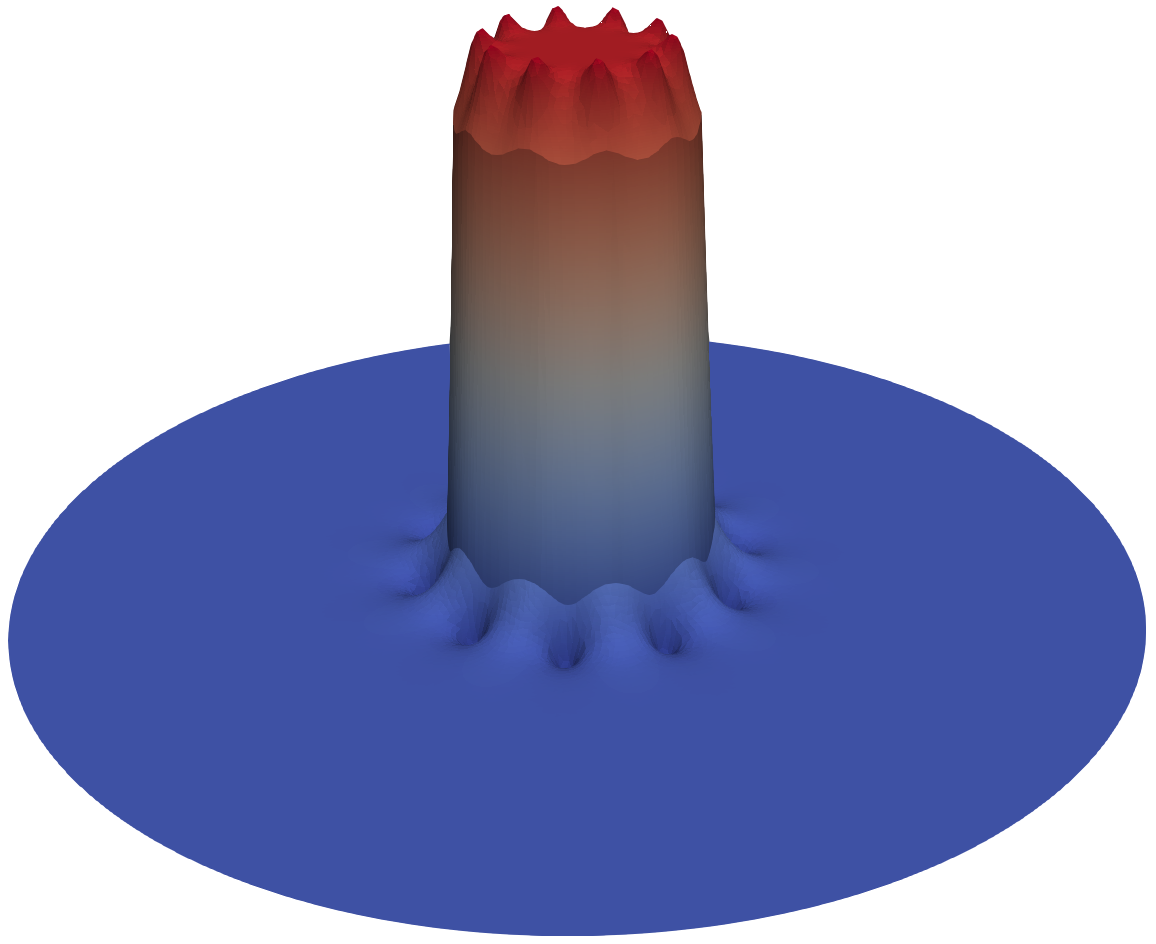
\includegraphics[width=0.95\linewidth]{fig/magnetostatics_potential.png}}
  \caption{
  Plot of the $z$-component $A_z$ of the magnetic vector potential. \label{ftut1:fig:magnetostatics:potential}
  }
\end{figure}
%\clearpage % flush figures ftut1:fig:magnetostatics:potential



\begin{figure}[!ht]  % ftut1:fig:magnetostatics:field
  \centerline{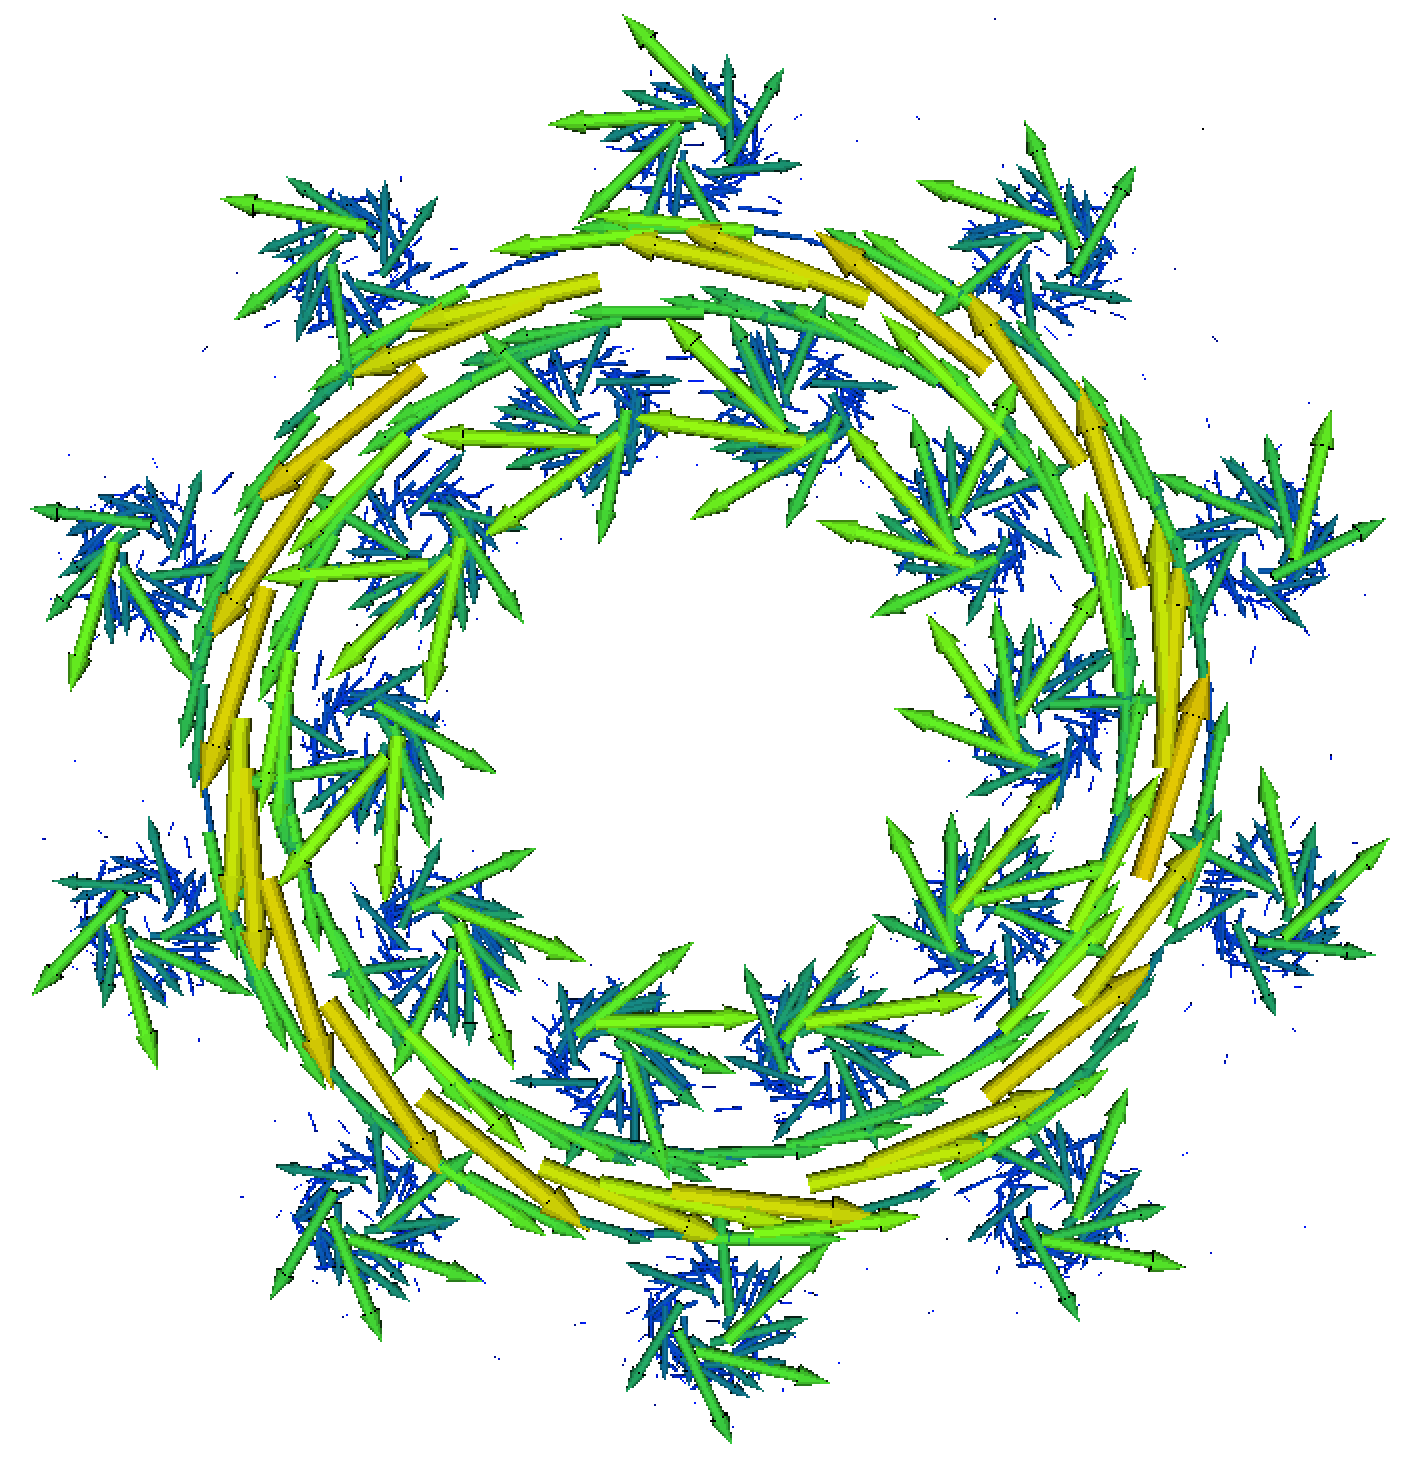
\includegraphics[width=0.75\linewidth]{fig/magnetostatics_field.png}}
  \caption{
  Plot of the magnetic field $B$ in the $xy$-plane. \label{ftut1:fig:magnetostatics:field}
  }
\end{figure}
%\clearpage % flush figures ftut1:fig:magnetostatics:field


The complete code for computing the magnetic field follows below.

\begin{lstlisting}[language=Python,style=graycolor]
from fenics import *
from mshr import *
from math import sin, cos, pi

a = 1.0   # inner radius of iron cylinder
b = 1.2   # outer radius of iron cylinder
c_1 = 0.8 # radius for inner circle of copper wires
c_2 = 1.4 # radius for outer circle of copper wires
r = 0.1   # radius of copper wires
R = 5.0   # radius of domain
n = 10    # number of windings

# Define geometry for background
domain = Circle(Point(0, 0), R)

# Define geometry for iron cylinder
cylinder = Circle(Point(0, 0), b) - Circle(Point(0, 0), a)

# Define geometry for wires (N = North (up), S = South (down))
angles_N = [i*2*pi/n for i in range(n)]
angles_S = [(i + 0.5)*2*pi/n for i in range(n)]
wires_N = [Circle(Point(c_1*cos(v), c_1*sin(v)), r) for v in angles_N]
wires_S = [Circle(Point(c_2*cos(v), c_2*sin(v)), r) for v in angles_S]

# Set subdomain for iron cylinder
domain.set_subdomain(1, cylinder)

# Set subdomains for wires
for (i, wire) in enumerate(wires_N):
    domain.set_subdomain(2 + i, wire)
for (i, wire) in enumerate(wires_S):
    domain.set_subdomain(2 + n + i, wire)

# Create mesh
mesh = generate_mesh(domain, 32)

# Define function space
V = FunctionSpace(mesh, 'P', 1)

# Define boundary condition
bc = DirichletBC(V, Constant(0), 'on_boundary')

# Define subdomain markers and integration measure
markers = MeshFunction('size_t', mesh, 2, mesh.domains())
dx = Measure('dx', domain=mesh, subdomain_data=markers)

# Define current densities
J_N = Constant(1.0)
J_S = Constant(-1.0)

# Define magnetic permeability
class Permeability(Expression):
    def __init__(self, mesh, **kwargs):
        self.markers = markers
    def eval_cell(self, values, x, cell):
        if markers[cell.index] == 0:
            values[0] = 4*pi*1e-7 # vacuum
        elif markers[cell.index] == 1:
            values[0] = 1e-5      # iron (should really be 2.5e-1)
        else:
            values[0] = -6.4e-6   # copper (yes, it's negative!)

mu = Permeability(mesh, degree=1)

# Define variational problem
A_z = TrialFunction(V)
v = TestFunction(V)
a = (1 / mu)*dot(grad(A_z), grad(v))*dx
L_N = sum(J_N*v*dx(i) for i in range(2, 2 + n))
L_S = sum(J_S*v*dx(i) for i in range(2 + n, 2 + 2*n))
L = L_N + L_S

# Solve variational problem
A_z = Function(V)
solve(a == L, A_z, bc)

# Compute magnetic field (B = curl A)
W = VectorFunctionSpace(mesh, 'P', 1)
B = project(as_vector((A_z.dx(1), -A_z.dx(0))), W)

# Plot solution
plot(A_z)
plot(B)

# Save solution to file
vtkfile_A_z = File('magnetostatics/potential.pvd')
vtkfile_B = File('magnetostatics/field.pvd')
vtkfile_A_z << A_z
vtkfile_B << B

# Hold plot
interactive()
\end{lstlisting}
This example program can be found in the file \href{{https://fenicsproject.org/pub/tutorial/python/vol1/ft11_magnetostatics.py}}{\nolinkurl{ft11_magnetostatics.py}}.

\index{ft11\_magnetostatics.py@{\rm\texttt{ft11\_magnetostatics.py}}}

% !split
\chapter{Extensions: Improving the Poisson solver}
\label{ch:poisson}


\begin{quote}
The FEniCS programs we have written so far have been designed as flat
Python scripts. This works well for solving simple demo
problems. However, when you build a solver for an advanced
application, you will quickly find the need for more structured
programming. In particular, you may want to reuse your solver to solve
a large number of problems where you vary the boundary conditions, the
domain, and coefficients such as material parameters. In this chapter,
we will see how to write general solver functions to improve the
usability of FEniCS programs. We will also discuss how to
utilize iterative solvers with preconditioners for solving linear
systems, how to compute derived quantities, such as, e.g., the flux
on a part of the boundary, and how to compute errors and convergence
rates.
\end{quote}


\section{Refactoring the Poisson solver}
\label{ch:poisson0:impl2}

\index{flat program}

Most programs discussed in this book are ``flat''; that is, they are
not organized into logical, reusable units in terms of Python
functions. Such flat programs are useful for quickly testing ideas and
sketching solution algorithms, but are not well suited for serious
problem solving. We shall therefore look at how to \emph{refactor} the
Poisson solver from Chapter~\ref{ch:fundamentals}. For a start, this
means splitting the code into functions. But refactoring is not just a
reordering of existing statements. During refactoring, we also try to
make the functions we create as reusable as possible in other
contexts. We will also encapsulate statements specific to a certain
problem into (non-reusable) functions. Being able to distinguish
reusable code from specialized code is a key issue when refactoring
code, and this ability depends on a good mathematical understanding of
the problem at hand (what is general, what is special?).  In a flat
program, general and specialized code (and mathematics) are often
mixed together, which tends to give a blurred understanding of the
problem at hand.

\subsection{A more general solver function}
\label{ch:poisson0:impl2:func}

We consider the flat program
\href{{https://fenicsproject.org/pub/tutorial/python/vol1/ft01_poisson.py}}{\nolinkurl{ft01_poisson.py}}
for solving the Poisson problem developed
in Chapter~\ref{ch:fundamentals}.
Some of the code in this program
is needed to solve any Poisson problem $-\nabla^2 u=f$ on $[0,1]\times
[0,1]$ with $u=\ub$ on the boundary, while other statements arise from
our simple test problem. Let us collect the general, reusable code in
a function called \texttt{solver}. Our special test problem will then just be
an application of our \texttt{solver} with some additional statements. We limit
the \texttt{solver} function to just \emph{compute the numerical
solution}. Plotting and comparing the solution with the exact solution
are considered to be problem-specific activities to be performed
elsewhere.

We parameterize \texttt{solver} by $f$, $\ub$, and the resolution of the
mesh. Since it is so trivial to use higher-order finite element
functions by changing the third argument to \texttt{FunctionSpace}, we
also add the polynomial degree of the finite element function space
as an argument to \texttt{solver}.

\begin{lstlisting}[language=Python,style=graycolor]
from fenics import *
import numpy as np

def solver(f, u_D, Nx, Ny, degree=1):
    """
    Solve -Laplace(u) = f on [0,1] x [0,1] with 2*Nx*Ny Lagrange
    elements of specified degree and u = u_D (Expresssion) on
    the boundary.
    """

    # Create mesh and define function space
    mesh = UnitSquareMesh(Nx, Ny)
    V = FunctionSpace(mesh, 'P', degree)

    # Define boundary condition
    def boundary(x, on_boundary):
        return on_boundary

    bc = DirichletBC(V, u_D, boundary)

    # Define variational problem
    u = TrialFunction(V)
    v = TestFunction(V)
    a = dot(grad(u), grad(v))*dx
    L = f*v*dx

    # Compute solution
    u = Function(V)
    solve(a == L, u, bc)

    return u
\end{lstlisting}

The remaining tasks of our initial program, such as calling the \texttt{solver}
function with problem-specific parameters and plotting,
can be placed in a separate function. Here we choose to put this code
in a function named \Verb!run_solver!:

\begin{lstlisting}[language=Python,style=graycolor]
def run_solver():
    "Run solver to compute and post-process solution"

    # Set up problem parameters and call solver
    u_D = Expression('1 + x[0]*x[0] + 2*x[1]*x[1]', degree=2)
    f = Constant(-6.0)
    u = solver(f, u_D, 8, 8, 1)

    # Plot solution and mesh
    plot(u)
    plot(u.function_space().mesh())

    # Save solution to file in VTK format
    vtkfile = File('poisson_solver/solution.pvd')
    vtkfile << u
\end{lstlisting}

The solution can now be computed, plotted, and saved to file by
simply calling the \Verb!run_solver! function.

\subsection{Writing the solver as a Python module}

\index{Python module}

The refactored code is placed in a file
\href{{https://fenicsproject.org/pub/tutorial/python/vol1/ft12_poisson_solver.py}}{\nolinkurl{ft12_poisson_solver.py}}.
We should make sure that such a file can be imported (and hence
reused) in other programs. This means that all statements in the main
program that are not inside functions should appear within a test
\Verb!if __name__ == '__main__':!. This test is true if the file is executed as
a program, but false if the file is imported.  If we want to run this
file in the same way as we can run \Verb!ft01_poisson.py!, the
main program is simply a call to \Verb!run_solver! followed by a call to
\texttt{interactive} to hold the plot:

\begin{lstlisting}[language=Python,style=graycolor]
if __name__ == '__main__':
    run_solver()
    interactive()
\end{lstlisting}
This complete program can be found in the file \href{{https://fenicsproject.org/pub/tutorial/python/vol1/ft12_poisson_solver.py}}{\nolinkurl{ft12_poisson_solver.py}}.

\index{ft12\_poisson\_solver.py@{\rm\texttt{ft12\_poisson\_solver.py}}}
\index{unit testing}

\subsection{Verification and unit tests}

\index{verification}

The remaining part of our first program is to compare the numerical
and the exact solutions. Every time we edit the code we must rerun the
test and examine that \Verb!error_max! is sufficiently small so we know
that the code still works. To this end, we shall adopt \emph{unit testing},
meaning that we create a mathematical test and corresponding software
that can run all our tests automatically and check that all tests
pass.  Python has several tools for unit testing. Two very popular
ones are pytest and nose. These are almost identical and very easy
to use.  More classical unit testing with test classes is offered by
the built-in module \texttt{unittest}, but here we are going to use pytest
(or nose) since that will result in shorter and clearer code.

Mathematically, our unit test is that the finite element solution of
our problem when $f=-6$ equals the exact solution $u=\ub=1+x^2+2y^2$
at the vertices of the mesh.
We have already created a code that finds the error at the vertices for
our numerical solution. Because of rounding errors, we cannot demand this
error to be zero, but we have to use a tolerance, which
depends on the number of elements and the degrees of the polynomials
in the finite element basis. If we want to test that the
\texttt{solver} function works for meshes up to $2\times(20\times 20)$
elements and cubic Lagrange elements, $10^{-10}$ is an appropriate
tolerance for testing that the maximum error vanishes.

To make our test case work together with pytest and nose, we have to
make a couple of small adjustments to our program. The simple
rule is that each test must be placed in a function that

\begin{itemize}
 \item has a name starting with \Verb!test_!,

 \item has no arguments, and

 \item implements a test expressed as \texttt{assert success, msg}.
\end{itemize}

\noindent
Regarding the last point, \texttt{success} is a boolean expression that is
\texttt{False} if the test fails, and in that case the string \texttt{msg} is
written to the screen. When the test fails, \texttt{assert} raises an
\texttt{AssertionError} exception in Python, and otherwise runs
silently. The \texttt{msg} string is optional, so \texttt{assert success} is the
minimal test. In our case, we will write \Verb!assert error_max < tol!,
where \texttt{tol} is the tolerance mentioned above.

A proper \emph{test function} for implementing this unit test in the
pytest or nose testing frameworks has the following form. Note
that we perform the test for different mesh resolutions and degrees of
finite elements.

\begin{lstlisting}[language=Python,style=graycolor]
def test_solver():
    "Test solver by reproducing u = 1 + x^2 + 2y^2"

    # Set up parameters for testing
    tol = 1E-10
    u_D = Expression('1 + x[0]*x[0] + 2*x[1]*x[1]', degree=2)
    f = Constant(-6.0)

    # Iterate over mesh sizes and degrees
    for Nx, Ny in [(3, 3), (3, 5), (5, 3), (20, 20)]:
        for degree in 1, 2, 3:
            print('Solving on a 2 x (%d x %d) mesh with P%d elements.'
                  % (Nx, Ny, degree))

            # Compute solution
            u = solver(f, u_D, Nx, Ny, degree)

            # Extract the mesh
            mesh = u.function_space().mesh()

            # Compute maximum error at vertices
            vertex_values_u_D = u_D.compute_vertex_values(mesh)
            vertex_values_u  = u.compute_vertex_values(mesh)
            error_max = np.max(np.abs(vertex_values_u_D - \
                                      vertex_values_u))

            # Check maximum error
            msg = 'error_max = %g' % error_max
            assert error_max < tol, msg
\end{lstlisting}

To run the test, we type the following command:

\begin{Verbatim}[frame=lines,label=\fbox{{\tiny Terminal}},framesep=2.5mm,framerule=0.7pt,fontsize=\fontsize{9pt}{9pt}]
Terminal> py.test ft12_poisson_solver.py
\end{Verbatim}
This will run all functions named \Verb!test_*! (currently only the
\Verb!test_solver! function) found in the file and report the results.
For more verbose output, add the flags \texttt{-s -v}.

We shall make it a habit to encapsulate numerical test problems in
unit tests as above, and we strongly encourage the reader to create
similar unit tests whenever a FEniCS solver is implemented.


\begin{notice_mdfboxadmon}[Tip: Print messages in test functions]
The \texttt{assert} statement runs silently when the test passes so users may
become uncertain if all the statements in a test function are really
executed. A psychological help is to print out something before \texttt{assert}
(as we do in the example above) such that it is clear that the
test really takes place.
Note that \texttt{py.test} needs the \texttt{-s} option to show printout
from the test functions.
\end{notice_mdfboxadmon} % title: Tip: Print messages in test functions




\begin{notice_mdfboxadmon}[Tip: Debugging with iPython]
One can easily enter iPython from a Python script by adding the following
line anywhere in the code:
\begin{lstlisting}[language=Python,style=graycolor]
from IPython import embed; embed()
\end{lstlisting}
This line starts an interactive Python session which lets you
print and plot variables, which can be very helpful for debugging.
\end{notice_mdfboxadmon} % title: Tip: Debugging with iPython

\subsection{Parameterizing the number of space dimensions}
\label{ch:poisson0:nD}
\index{dimension-independent code}

\index{space dimensions}

FEniCS makes it is easy to write a unified simulation code that can
operate in 1D, 2D, and 3D. As an appetizer, go back to the
previous programs
\href{{https://fenicsproject.org/pub/tutorial/python/vol1/ft01_poisson.py}}{\nolinkurl{ft01_poisson.py}}
or
\href{{https://fenicsproject.org/pub/tutorial/python/vol1/ft12_poisson_solver.py}}{\nolinkurl{ft12_poisson_solver.py}}
and change the mesh construction from \texttt{UnitSquareMesh(8, 8)} to
\texttt{UnitCubeMesh(8, 8, 8)}. Now the domain is the unit cube
partitioned into $8\times 8\times 8$ boxes, and each box
is divided into six tetrahedron-shaped finite elements for
computations. Run the program and observe that we can solve a 3D
problem without any other modifications! (In 1D, expressions must be
modified to not depend on \texttt{x[1]}.) The visualization allows you to
rotate the cube and observe the function values as colors on the
boundary.

If we want to parameterize the creation of unit interval, unit square,
or unit cube over dimension, we can do so by encapsulating this part
of the code in a function. Given a list or tuple specifying the division
into cells in the spatial coordinates, the following function
returns the mesh for a $d$-dimensional cube:

\begin{lstlisting}[language=Python,style=graycolor]
def UnitHyperCube(divisions):
    mesh_classes = [UnitIntervalMesh, UnitSquareMesh, UnitCubeMesh]
    d = len(divisions)
    mesh = mesh_classes[d - 1](*divisions)
    return mesh
\end{lstlisting}
The construction \Verb!mesh_class[d - 1]! will pick the right name of the
object used to define the domain and generate the mesh.  Moreover, the
argument \texttt{*divisions} sends all the components of the list \texttt{divisions}
as separate arguments to the constructor of the mesh construction
class picked out by \Verb!mesh_class[d - 1]!. For example, in a 2D problem
where \texttt{divisions} has two elements, the statement

\begin{lstlisting}[language=Python,style=graycolor]
mesh = mesh_classes[d - 1](*divisions)
\end{lstlisting}
is equivalent to

\begin{lstlisting}[language=Python,style=graycolor]
mesh = UnitSquareMesh(divisions[0], divisions[1])
\end{lstlisting}

The \texttt{solver} function from
\href{{https://fenicsproject.org/pub/tutorial/python/vol1/ft12_poisson_solver.py}}{\nolinkurl{ft12_poisson_solver.py}}
may be modified to solve $d$-dimensional problems by replacing the
\texttt{Nx} and \texttt{Ny} parameters by \texttt{divisions}, and calling the function
\texttt{UnitHyperCube} to create the mesh. Note that \texttt{UnitHyperCube} is a
\emph{function} and not a \emph{class}, but we have named it using so-called
\emph{CamelCase notation} to make it look like a class:

\begin{lstlisting}[language=Python,style=graycolor]
mesh = UnitHyperCube(divisions)
\end{lstlisting}

% !split
\section{Working with linear solvers}
\label{ch:poisson0:solve:prm}

Sparse LU decomposition (Gaussian elimination) is used by default to
solve linear systems of equations in FEniCS programs.  This is a very
robust and simple method. It is the recommended method for systems
with up to a few thousand unknowns and may hence be the method of
choice for many 2D and smaller 3D problems. However, sparse LU
decomposition becomes slow and one quickly runs out of memory for
larger problems. For large problems, we instead need to use \emph{iterative
methods} which are faster and require much less memory. We will now
look at how to take advantage of state-of-the-art iterative solution
methods in FEniCS.

\subsection{Choosing a linear solver and preconditioner}

\index{linear solver}
\index{preconditioner}
\index{Krylov solver}

Preconditioned Krylov solvers is a type of popular iterative methods
that are easily accessible in FEniCS programs. The Poisson equation
results in a symmetric, positive definite system matrix, for which the
optimal Krylov solver is the Conjugate Gradient (CG) method. For
non-symmetric problems, a Krylov solver for non-symmetric systems,
such as GMRES, is a better choice. Incomplete LU factorization (ILU)
is a popular and robust all-round preconditioner, so let us try the
GMRES-ILU pair:

\begin{lstlisting}[language=Python,style=graycolor]
solve(a == L, u, bc,
      solver_parameters={'linear_solver': 'gmres',
                         'preconditioner': 'ilu'})
# Alternative syntax
solve(a == L, u, bc,
      solver_parameters=dict(linear_solver='gmres',
                             preconditioner='ilu'))
\end{lstlisting}
Section~\ref{ftut:app:solver:prec} lists the most popular choices of
Krylov solvers and preconditioners available in FEniCS.

\index{linear algebra backend}
\index{PETSc} \index{Eigen}

\subsection{Choosing a linear algebra backend}

The actual GMRES and ILU implementations that are brought into action
depend on the choice of linear algebra package. FEniCS interfaces
several linear algebra packages, called \emph{linear algebra backends} in
FEniCS terminology. PETSc is the default choice if FEniCS is compiled
with PETSc. If PETSc is not available, then FEniCS falls back to using
the Eigen backend. The linear algebra backend in FEniCS can be set
using the following command:

\begin{lstlisting}[language=Python,style=graycolor]
parameters.linear_algebra_backend = backendname
\end{lstlisting}
where \texttt{backendname} is a string. To see which linear algebra backends
are available, you can call the FEniCS function
\Verb!list_linear_algebra_backends!. Similarly, one may check which
linear algebra backend is currently being used by the following
command:

\begin{lstlisting}[language=Python,style=graycolor]
print(parameters.linear_algebra_backend)
\end{lstlisting}

\index{parameters@{\rm\texttt{parameters}}}
\index{info@{\rm\texttt{info}}}

\subsection{Setting solver parameters}

We will normally want to control the tolerance in the stopping
criterion and the maximum number of iterations when running an
iterative method. Such parameters can be controlled at both a \emph{global}
and a \emph{local} level. We will start by looking at how to set global
parameters. For more advanced programs, one may want to use a number
of different linear solvers and set different tolerances and other
parameters. Then it becomes important to control the parameters at a
\emph{local} level. We will return to this issue in Section~\ref{ch:poisson0:solver:problem}.

Changing a parameter in the global FEniCS parameter database affects
all linear solvers (created \emph{after} the parameter has been set).
The global FEniCS parameter database is simply called \texttt{parameters} and
it behaves as a nested dictionary. Write

\begin{lstlisting}[language=Python,style=graycolor]
info(parameters, verbose=True)
\end{lstlisting}
to list all parameters and their default values in the database.
The nesting of parameter sets is indicated through indentation in the
output from \texttt{info}.
According to this output, the relevant parameter set is
named \Verb!'krylov_solver'!, and the parameters are set like this:

\begin{lstlisting}[language=Python,style=graycolor]
prm = parameters.krylov_solver  # short form
prm.absolute_tolerance = 1E-10
prm.relative_tolerance = 1E-6
prm.maximum_iterations = 1000
\end{lstlisting}
Stopping criteria for Krylov solvers usually involve some norm of
the residual, which must be smaller than the absolute tolerance
parameter \emph{or} smaller than the relative tolerance parameter times
the initial residual.

% To get a printout of the number of actual iterations to reach the
% topping criterion, we can insert
%
% !bc pycod
% set_log_level(PROGRESS)
% set_log_level(DEBUG)
% !ec
% A message with the equation system size, solver type, and number of
% iterations arises from specifying the argument \texttt{PROGRESS}, while
% \texttt{DEBUG} results in more information, including CPU time spent in
% the various parts of the matrix assembly and solve process.

We remark that default values for the global parameter database can be
defined in an XML file. To generate such a file from the current set
of parameters in a program, run

\begin{lstlisting}[language=Python,style=graycolor]
File('parameters.xml') << parameters
\end{lstlisting}
If a \Verb!dolfin_parameters.xml! file is found in the directory where a
FEniCS program is run, this file is read and used to initialize the
\texttt{parameters} object. Otherwise, the file
\Verb!.config/fenics/dolfin_parameters.xml! in the user's home directory is
read, if it exists.  Another alternative is to load the XML file (with any
name) manually in the program:

\begin{lstlisting}[language=Python,style=graycolor]
File('parameters.xml') >> parameters
\end{lstlisting}
The XML file can also be in gzip'ed form with the extension \texttt{.xml.gz}.

\subsection{An extended solver function}

We may extend the previous solver function from
\href{{https://fenicsproject.org/pub/tutorial/python/vol1/ft12_poisson_solver.py}}{\nolinkurl{ft12_poisson_solver.py}}
in Section~\ref{ch:poisson0:impl2:func}
such that it also offers the GMRES+ILU
preconditioned Krylov solver:

% @@@CODE vol1/python/poisson_extended.py fromto: def solver(@def solver_objects

\index{ft10\_poisson\_extended.py@{\rm\texttt{ft10\_poisson\_extended.py}}}

This new \texttt{solver} function, found in the file
\href{{https://fenicsproject.org/pub/tutorial/python/vol1/ft10_poisson_extended.py}}{\nolinkurl{ft10_poisson_extended.py}},
replaces the one in
\href{{https://fenicsproject.org/pub/tutorial/python/vol1/ft12_poisson_solver.py}}{\nolinkurl{ft12_poisson_solver.py}}.
It has all the functionality of the previous \texttt{solver} function, but
can also solve the linear system with iterative methods.

\subsection{A remark regarding unit tests}

Regarding verification of the new \texttt{solver} function in terms of unit
tests, it turns out that unit testing for a problem where the
approximation error vanishes gets more complicated when we use
iterative methods. The problem is to keep the error due to iterative
solution smaller than the tolerance used in the verification
tests. First of all, this means that the tolerances used in the Krylov
solvers must be smaller than the tolerance used in the \texttt{assert} test,
but this is no guarantee to keep the linear solver error this small.
For linear elements and small meshes, a tolerance of $10^{-11}$ works
well in the case of Krylov solvers too (using a tolerance $10^{-12}$
in those solvers). The interested reader is referred to the
\Verb!demo_solvers! function in
\href{{https://fenicsproject.org/pub/tutorial/python/vol1/ft10_poisson_extended.py}}{\nolinkurl{ft10_poisson_extended.py}}
for details:
this function tests the numerical solution for direct and iterative
linear solvers, for different meshes, and different degrees of the
polynomials in the finite element basis functions.

\subsection{List of linear solver methods and preconditioners}
\label{ftut:app:solver:prec}

\index{linear solver}
\index{Krylov solver}
\index{preconditioner}

Which linear solvers and preconditioners that are available
in FEniCS depends on how FEniCS has been configured and which
linear algebra backend is currently active. The following table
shows an example of which linear solvers that can be available
through FEniCS when the PETSc backend is active:

{\small   % for Springer style: small table font and more vspace

\vspace{4mm}

\begin{tabular}{ll}
\hline\noalign{\smallskip}
\multicolumn{1}{c}{ Name } & \multicolumn{1}{c}{ Method } \\
\noalign{\smallskip}\svhline\noalign{\smallskip}
\texttt{'bicgstab'}     & Biconjugate gradient stabilized method       \\
\texttt{'cg'}           & Conjugate gradient method                    \\
\texttt{'gmres'}        & Generalized minimal residual method          \\
\texttt{'minres'}       & Minimal residual method                      \\
\texttt{'petsc'}        & PETSc built in LU solver                     \\
\texttt{'richardson'}   & Richardson method                            \\
\Verb!'superlu_dist'! & Parallel SuperLU                             \\
\texttt{'tfqmr'}        & Transpose-free quasi-minimal residual method \\
\texttt{'umfpack'}      & UMFPACK                                      \\
\noalign{\smallskip}\hline\noalign{\smallskip}
\end{tabular}

\vspace{4mm}

}

\noindent
The set of available preconditioners also depends on configuration and
linear algebra backend. The following table shows an example of which
preconditioners may be available:



{\small   % for Springer style: small table font and more vspace

\vspace{4mm}

\begin{tabular}{ll}
\hline\noalign{\smallskip}
\multicolumn{1}{c}{ Name } & \multicolumn{1}{c}{ Method } \\
\noalign{\smallskip}\svhline\noalign{\smallskip}
\texttt{'icc'}       & Incomplete Cholesky factorization \\
\texttt{'ilu'}       & Incomplete LU factorization       \\
\Verb!'petsc_amg'! & PETSc algebraic multigrid         \\
\texttt{'sor'}       & Successive over-relaxation        \\
\noalign{\smallskip}\hline\noalign{\smallskip}
\end{tabular}

\vspace{4mm}

}


\noindent
An up-to-date list of the available solvers and preconditioners
for your FEniCS installation can be produced by

\begin{lstlisting}[language=Python,style=graycolor]
list_linear_solver_methods()
list_krylov_solver_preconditioners()
\end{lstlisting}

% !split
\section{High-level and low-level solver interfaces}

The FEniCS interface allows different ways to access the core
functionality, ranging from very high-level to low-level access. So
far, we have mostly used the high-level call \texttt{solve(a == L, u, bc)} to
solve a variational problem \texttt{a == L} with a certain boundary condition
\texttt{bc}. However, sometimes you may need more fine-grained control of
the solution process. In particular, the call to \texttt{solve} will create
certain objects that are thrown away after the solution has been
computed, and it may be practical or efficient to \emph{reuse} those
objects.

\subsection{Linear variational problem and solver objects}
\label{ch:poisson0:solver:problem}
\index{LinearVariationalProblem}
\index{LinearVariationalSolver}

In this section, we will look at an alternative interface to solving
linear variational problems in FEniCS, which may be preferable in
many situations compared to the high-level \texttt{solve} function interface.
This interface uses the two classes \texttt{LinearVariationalProblem} and
\texttt{LinearVariationalSolver}. Using this interface, the equivalent of
\texttt{solve(a == L, u, bc)} looks as follows:

\begin{lstlisting}[language=Python,style=graycolor]
u = Function(V)
problem = LinearVariationalProblem(a, L, u, bc)
solver = LinearVariationalSolver(problem)
solver.solve()
\end{lstlisting}

Many FEniCS objects have an attribute \texttt{parameters}, similar to
the global \texttt{parameters} database,
but local to the object. Here, \texttt{solver.parameters} play that
role. Setting the CG method with ILU preconditioning as the solution
method and specifying solver-specific parameters can be done
like this:

\begin{lstlisting}[language=Python,style=graycolor]
solver.parameters.linear_solver = 'gmres'
solver.parameters.preconditioner = 'ilu'
prm = solver.parameters.krylov_solver  # short form
prm.absolute_tolerance = 1E-7
prm.relative_tolerance = 1E-4
prm.maximum_iterations = 1000
\end{lstlisting}
Settings in the global \texttt{parameters} database are
propagated to parameter sets in individual objects, with the
possibility of being overwritten as above. Note that global parameter
values can only affect local parameter values if set before the time
of creation of the local object. Thus, changing the value of the
tolerance in the global parameter database will not affect the
parameters for already created solvers.

\subsection{Explicit assembly and solve}
\label{ch:poisson0:linalg}

\index{assembly}
\index{assemble@{\rm\texttt{assemble}}}

As we saw already in Section~\ref{ftut1:NS}, linear variational
problems can be assembled explicitly in FEniCS into matrices and
vectors using the \texttt{assemble} function. This allows even more
fine-grained control of the solution process compared to using the
high-level \texttt{solve} function or using the classes
\texttt{LinearVariationalProblem} and
\texttt{LinearVariationalSolver}. We will now look more closely into how to
use the \texttt{assemble} function and how to combine this with low-level
calls for solving the assembled linear systems.

Given a variational problem $a(u,v)=L(v)$, the discrete solution $u$
is computed by inserting $u=\sum_{j=1}^N U_j \phi_j$ into $a(u,v)$ and
demanding $a(u,v)=L(v)$ to be fulfilled for $N$ test functions
$\hat\phi_1,\ldots,\hat\phi_N$. This implies

\begin{equation*}
\sum_{j=1}^N a(\phi_j,\hat\phi_i) U_j = L(\hat\phi_i),\quad i=1,\ldots,N,
\end{equation*}
which is nothing but a linear system,

\begin{equation*}
  AU = b,
\end{equation*}
where the entries of $A$ and $b$ are given by

\begin{align*}
  A_{ij} &= a(\phi_j, \hat{\phi}_i), \\
  b_i &= L(\hat\phi_i)\tp
\end{align*}

\index{assemble@{\rm\texttt{assemble}}}
\index{linear system}

The examples so far have specified the left- and right-hand sides of
the variational formulation and then asked FEniCS to assemble the
linear system and solve it. An alternative is to explicitly call
functions for assembling the coefficient matrix $A$ and the right-hand
side vector $b$, and then solve the linear system $AU=b$ for
the vector $U$. Instead of \texttt{solve(a == L, U, b)} we now write

\begin{lstlisting}[language=Python,style=graycolor]
A = assemble(a)
b = assemble(L)
bc.apply(A, b)
u = Function(V)
U = u.vector()
solve(A, U, b)
\end{lstlisting}
The variables \texttt{a} and \texttt{L} are the same as before; that is, \texttt{a} refers
to the bilinear form involving a \texttt{TrialFunction} object \texttt{u}
and a \texttt{TestFunction} object \texttt{v}, and \texttt{L} involves the same \texttt{TestFunction}
object \texttt{v}. From \texttt{a} and \texttt{L}, the \texttt{assemble} function can compute
$A$ and $b$.

Creating the linear system explicitly in a program can have some
advantages in more advanced problem settings. For example, $A$ may
be constant throughout a time-dependent simulation, so we can avoid
recalculating $A$ at every time level and save a significant amount
of simulation time.

The matrix $A$ and vector $b$ are first assembled without
incorporating essential (Dirichlet) boundary conditions. Thereafter,
the call \texttt{bc.apply(A, b)} performs the necessary modifications of the
linear system such that \texttt{u} is guaranteed to equal the prescribed
boundary values. When we have multiple Dirichlet conditions stored in
a list \texttt{bcs}, we must apply each condition in \texttt{bcs} to the system:

\begin{lstlisting}[language=Python,style=graycolor]
for bc in bcs:
    bc.apply(A, b)

# Alternative syntax using list comprehension
[bc.apply(A, b) for bc in bcs]
\end{lstlisting}

\index{assemble\_system@{\rm\texttt{assemble\_system}}}

Alternatively, we can use the function \Verb!assemble_system!, which takes
the boundary conditions into account when assembling the linear
system. This method preserves the symmetry of the linear system for a
symmetric bilinear form. Even if the matrix \texttt{A} that comes out
of the call to \texttt{assemble} is symmetric (for a symmetric bilinear form
\texttt{a}), the call to \texttt{bc.apply} will break the symmetry. Preserving the
symmetry of a variational problem is important when using particular
linear solvers designed for symmetric systems, such as the conjugate
gradient method.

% That is, for each degree of freedom
% that is known, the corresponding row and column is zero'ed out and 1
% is placed on the main diagonal, and the right-hand side \texttt{b} is
% modified by subtracting the column in \texttt{A} times the value of the
% degree of, and then the corresponding entry in \texttt{b} is replaced by the
% known value of the degree of freedom.
% With \texttt{bc.apply(A, b)} the
% matrix \texttt{A} is modified in an nonsymmetric way.
% : The row is zero'ed out
% and 1 is placed on the main diagonal, and the degree of freedom value
% is inserted in \texttt{b}.

Once the linear system has been assembled, we need to compute the
solution $U=A^{-1}b$ and store the solution $U$ in the vector
\texttt{U = u.vector()}. In the same way as linear variational problems can be
programmed using different interfaces in FEniCS---the high-level
\texttt{solve} function, the class \texttt{LinearVariationalSolver}, and the
low-level \texttt{assemble} function---linear systems can also be programmed
using different interfaces in FEniCS. The high-level interface to
solving a linear system in FEniCS is also named \texttt{solve}:

\begin{lstlisting}[language=Python,style=graycolor]
solve(A, U, b)
\end{lstlisting}

By default, \texttt{solve(A, U, b)} uses sparse LU decomposition to compute
the solution. Specification of an iterative solver and preconditioner
can be made through two optional arguments:

\begin{lstlisting}[language=Python,style=graycolor]
solve(A, U, b, 'cg', 'ilu')
\end{lstlisting}
Appropriate names of solvers and preconditioners are found in
Section~\ref{ftut:app:solver:prec}.

\index{KrylovSolver@{\rm\texttt{KrylovSolver}}}

This high-level interface is useful for many applications, but
sometimes more fine-grained control is needed. One can then create one
or more \texttt{KrylovSolver} objects that are then used to solve linear
systems. Each different solver object can have its own set of
parameters and selection of iterative method and preconditioner. Here
is an example:

\begin{lstlisting}[language=Python,style=graycolor]
solver = KrylovSolver('cg', 'ilu')
prm = solver.parameters
prm.absolute_tolerance = 1E-7
prm.relative_tolerance = 1E-4
prm.maximum_iterations = 1000
u = Function(V)
U = u.vector()
solver.solve(A, U, b)
\end{lstlisting}
The function \Verb!solver_linalg! in the program file
\href{{https://fenicsproject.org/pub/tutorial/python/vol1/ft10_poisson_extended.py}}{\nolinkurl{ft10_poisson_extended.py}}
implements such a solver.

The choice of start vector for the iterations in a linear solver is
often important. By default, the values of \texttt{u} and thus the vector \texttt{U = u.vector()} will be initialized to zero. If we instead wanted to
initialize \texttt{U} with random numbers in the interval $[-100,100]$ this
can be done as follows:

\begin{lstlisting}[language=Python,style=graycolor]
n = u.vector().array().size
U = u.vector()
U[:] = numpy.random.uniform(-100, 100, n)
solver.parameters.nonzero_initial_guess = True
solver.solve(A, U, b)
\end{lstlisting}
Note that we must both turn off the default behavior of setting the start
vector (``initial guess'') to zero, and also set the values of the
vector \texttt{U} to nonzero values. This is useful if we happen to
know a good initial guess for the solution.

Using a nonzero initial guess can be particularly important for
time-dependent problems or when solving a linear system as part of a
nonlinear iteration, since then the previous solution vector \texttt{U} will
often be a good initial guess for the solution in the next time step
or iteration. In this case, the values in the vector \texttt{U} will
naturally be initialized with the previous solution vector (if we just
used it to solve a linear system), so the only extra step necessary is
to set the parameter \Verb!nonzero_initial_guess! to \texttt{True}.

% In other problems, we may divide the variational
% problem and linear system into different terms, say $A=M + {\dt} K$,
% where $M$ is a matrix arising from a term like $\partial u/\partial t$,
% $K$ is a term corresponding to a Laplace operator, and $\dt$ is
% a time discretization parameter. When $\dt$ is changed in time,
% we can efficiently recompute $A = M + {\dt} K$ without
% reassembling the constant matrices $M$ and $K$. This strategy may
% speed up simulations significantly.

\subsection{Examining matrix and vector values}

When calling \texttt{A = assemble(a)} and \texttt{b = assemble(L)}, the object \texttt{A}
will be of type \texttt{Matrix}, while \texttt{b} and \texttt{u.vector()} are of type
\texttt{Vector}. To examine the values, we may convert the matrix and vector
data to \texttt{numpy} arrays by calling the \texttt{array} method as shown
before. For example, if you wonder how essential boundary conditions are
incorporated into linear systems, you can print out \texttt{A} and \texttt{b}
before and after the \texttt{bc.apply(A, b)} call:

\begin{lstlisting}[language=Python,style=graycolor]
A = assemble(a)
b = assemble(L)
if mesh.num_cells() < 16:  # print for small meshes only
    print(A.array())
    print(b.array())
bc.apply(A, b)
if mesh.num_cells() < 16:
    print(A.array())
    print(b.array())
\end{lstlisting}

With access to the elements in \texttt{A} through a \texttt{numpy} array, we can easily
perform computations on this matrix, such as computing the eigenvalues
(using the \texttt{eig} function in \texttt{numpy.linalg}). We can alternatively dump
\texttt{A.array()} and \texttt{b.array()} to file in MATLAB format and invoke
MATLAB or Octave to analyze the linear system.
Dumping the arrays to MATLAB format is done by

\index{MATLAB}

\begin{lstlisting}[language=Python,style=graycolor]
import scipy.io
scipy.io.savemat('Ab.mat', {'A': A.array(), 'b': b.array()})
\end{lstlisting}
Writing \texttt{load Ab.mat} in MATLAB or Octave will then make
the array variables \texttt{A} and \texttt{b} available for computations.

\index{SLEPc}

Matrix processing in Python or MATLAB/Octave is only feasible for
small PDE problems since the \texttt{numpy} arrays or matrices in MATLAB file
format are dense matrices. FEniCS also has an interface to the
eigensolver package SLEPc, which is the preferred tool for computing
the eigenvalues of large, sparse matrices of the type encountered in
PDE problems (see \texttt{demo/documented/eigenvalue/python/} in the
FEniCS/DOLFIN source code tree for a demo).

% !split
\section{Degrees of freedom and function evaluation}

\subsection{Examining the degrees of freedom}
\label{ch:poisson0:verify1}

\index{degrees of freedrom}
\index{vertex values}
\index{coordinates}

We have seen before how to grab the degrees of freedom array from a
finite element function \texttt{u}:

\begin{lstlisting}[language=Python,style=graycolor]
nodal_values = u.vector().array()
\end{lstlisting}

For a finite element function from a standard continuous piecewise linear
function space ($\mathsf{P}_1$ Lagrange elements), these values will
be the same as the values we get by the following statement:

\begin{lstlisting}[language=Python,style=graycolor]
vertex_values = u.compute_vertex_values(mesh)
\end{lstlisting}
Both \Verb!nodal_values! and \Verb!vertex_values! will be \texttt{numpy} arrays and
they will be of the same length and contain the same values (for
$\mathsf{P}_1$ elements), but with possibly different ordering. The
array \Verb!vertex_values! will have the same ordering as the vertices of
the mesh, while \Verb!nodal_values! will be ordered in a way that (nearly)
minimizes the bandwidth of the system matrix and thus improves the
efficiency of linear solvers.

A fundamental question is: what are the
coordinates of the vertex whose value is \Verb!nodal_values[i]!? To answer this
question, we need to understand how to get our hands on the
coordinates, and in particular, the numbering of degrees of freedom
and the numbering of vertices in the mesh.

The function \texttt{mesh.coordinates} returns the coordinates of the
vertices as a \texttt{numpy} array with shape ($M,d$), $M$ being the number
of vertices in the mesh and $d$ being the number of space dimensions:

\begin{lstlisting}[language=Python,style=graycolor]
>>> from fenics import *
>>> mesh = UnitSquareMesh(2, 2)
>>> coordinates = mesh.coordinates()
>>> coordinates
array([[ 0. ,  0. ],
       [ 0.5,  0. ],
       [ 1. ,  0. ],
       [ 0. ,  0.5],
       [ 0.5,  0.5],
       [ 1. ,  0.5],
       [ 0. ,  1. ],
       [ 0.5,  1. ],
       [ 1. ,  1. ]])
\end{lstlisting}
We see from this output that for this particular mesh, the vertices
are first numbered along $y=0$
with increasing $x$ coordinate, then along $y=0.5$, and so on.

Next we compute a function \texttt{u} on this mesh. Let's take $u=x+y$:

\begin{lstlisting}[language=Python,style=graycolor]
>>> V = FunctionSpace(mesh, 'P', 1)
>>> u = interpolate(Expression('x[0] + x[1]', degree=1), V)
>>> plot(u, interactive=True)
>>> nodal_values = u.vector().array()
>>> nodal_values
array([ 1. ,  0.5,  1.5,  0. ,  1. ,  2. ,  0.5,  1.5,  1. ])
\end{lstlisting}
We observe that \Verb!nodal_values[0]! is \emph{not} the value of $x+y$ at
vertex number 0, since this vertex has coordinates $x=y=0$. The
numbering of the nodal values (degrees of freedom) $U_1,\ldots,U_{N}$
is obviously not the same as the numbering of the vertices.

The vertex numbering may be examined by using the FEniCS \texttt{plot}
command. To do this, plot the function \texttt{u}, press \texttt{w} to turn on
wireframe instead of a fully colored surface, \texttt{m} to show the mesh,
and then \texttt{v} to show the numbering of the vertices.



\vspace{6mm}

% inline figure
\centerline{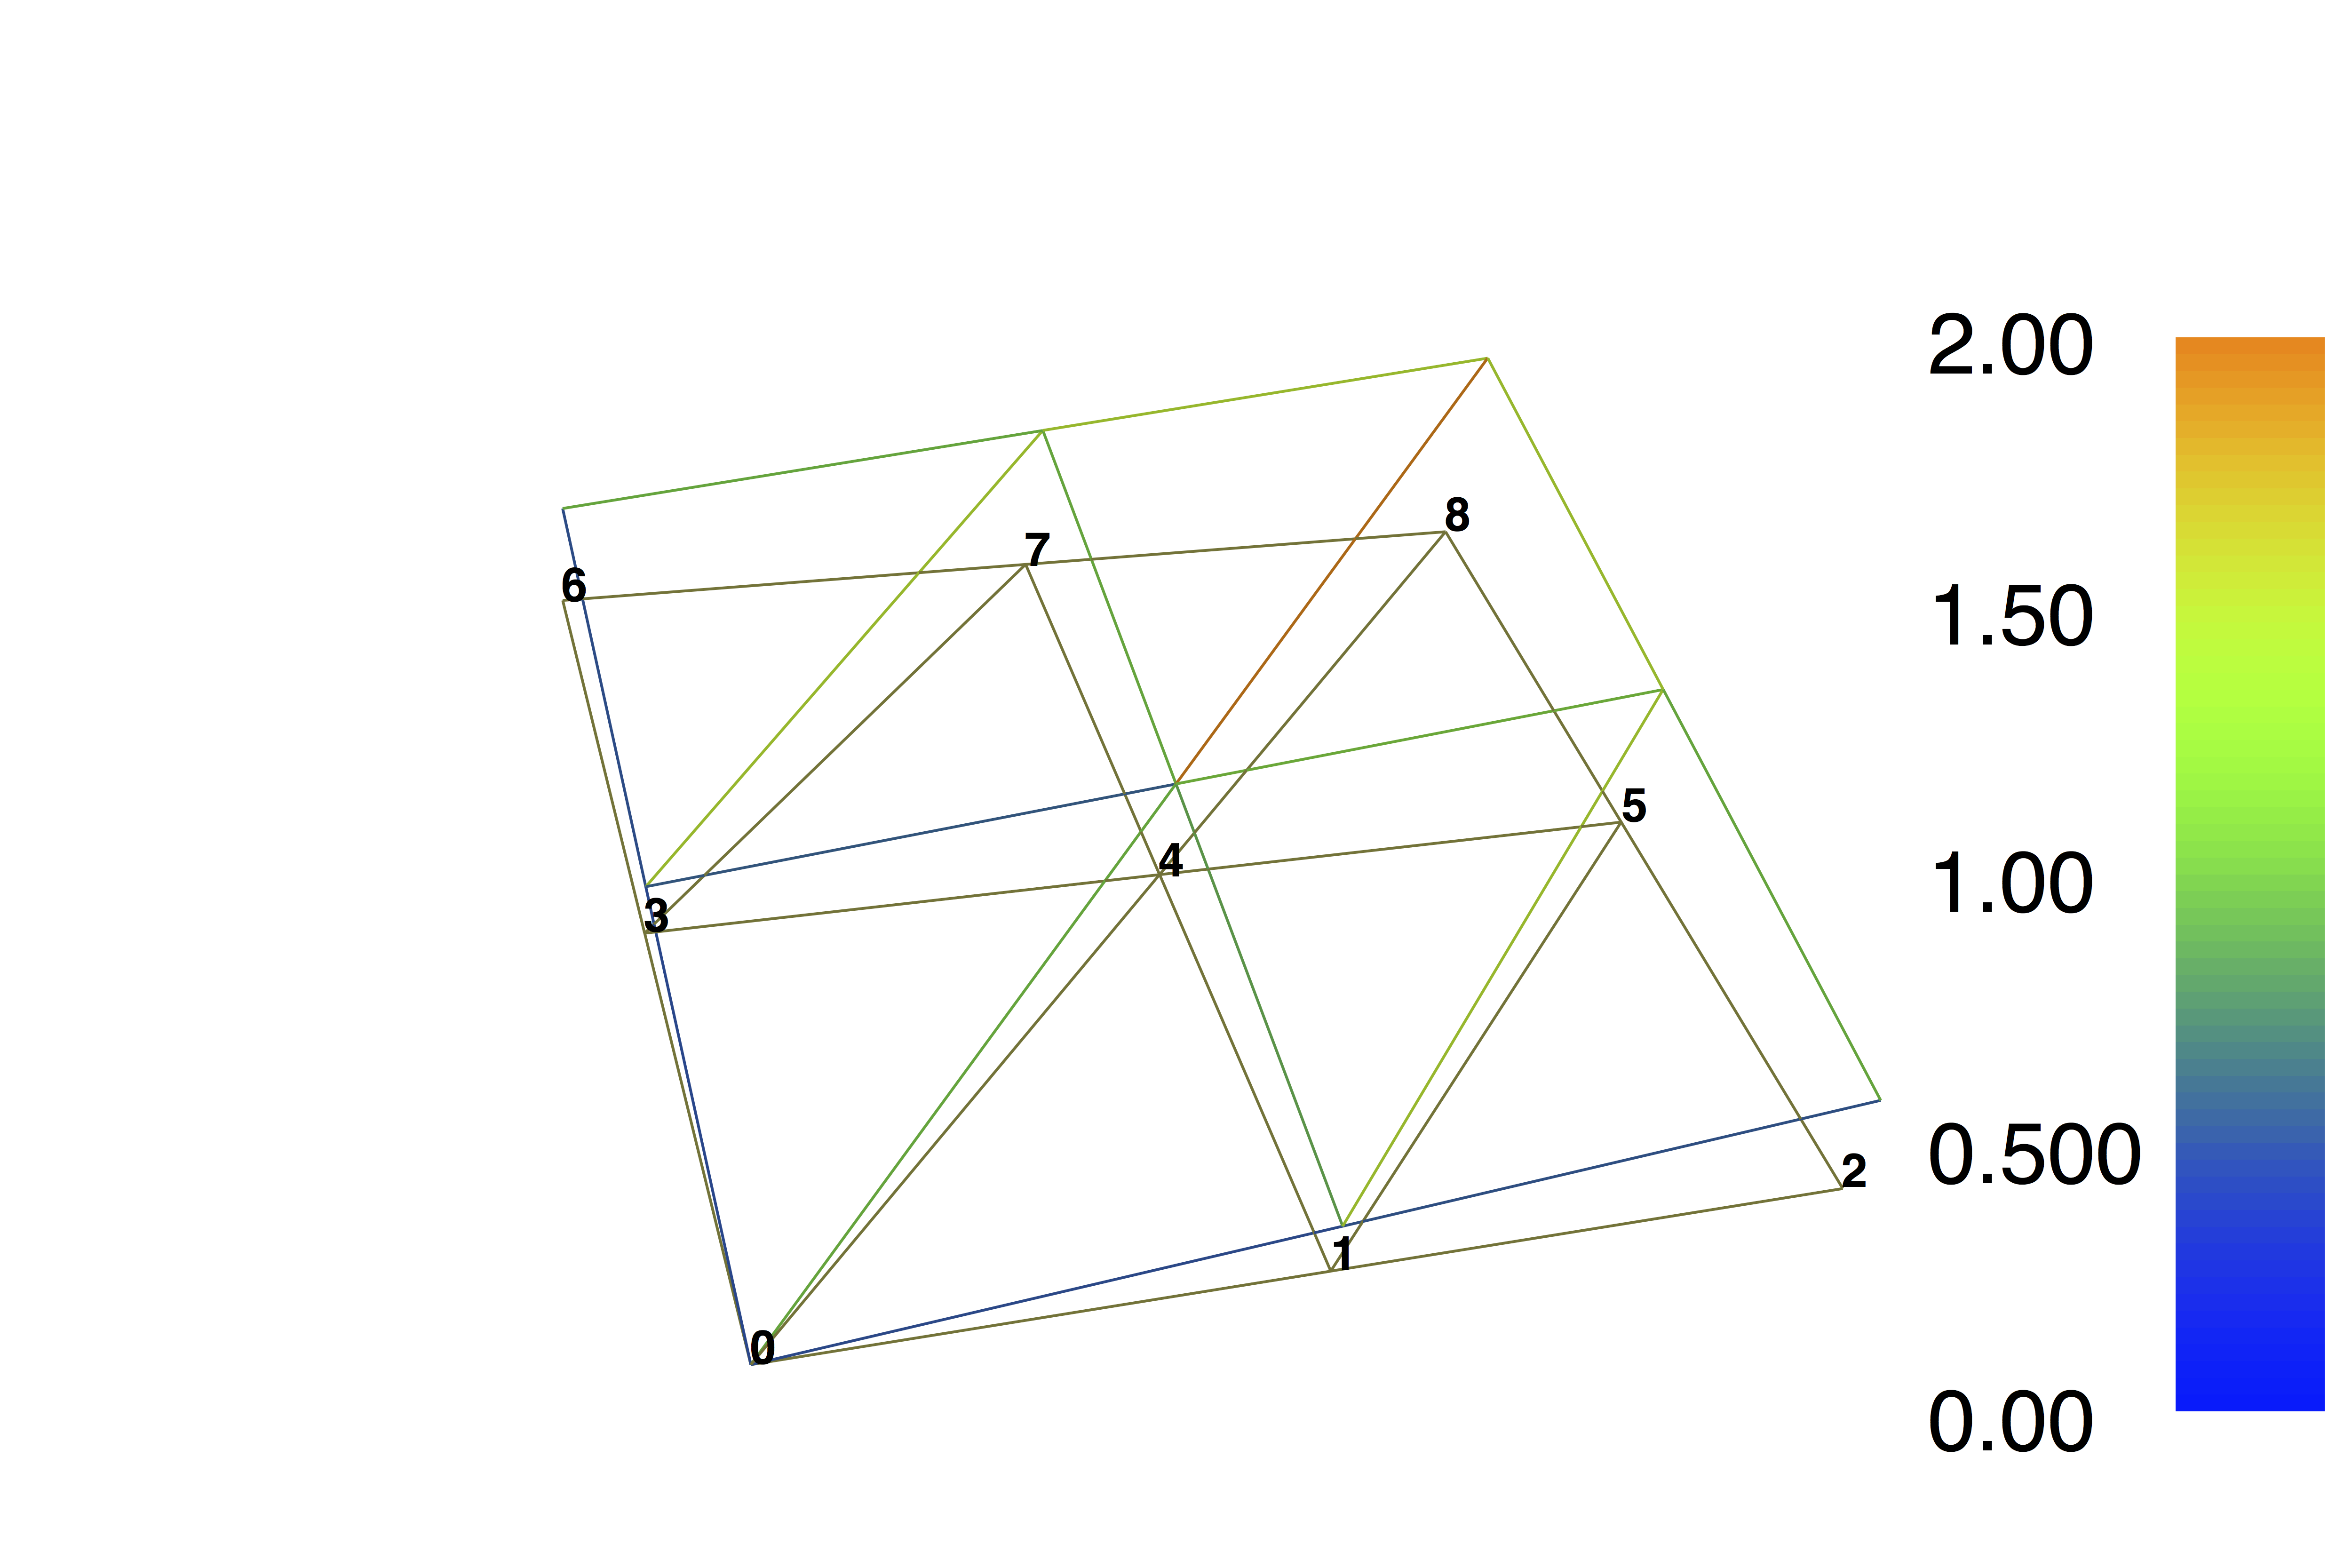
\includegraphics[width=0.75\linewidth]{fig/vertex_numbering.png}}

\vspace{6mm}



\index{vertex values}

Let's instead examine the values by calling
\Verb!u.compute_vertex_values!:

\begin{lstlisting}[language=Python,style=graycolor]
>>> vertex_values = u.compute_vertex_values()
>>> for i, x in enumerate(coordinates):
...     print('vertex %d: vertex_values[%d] = %g\tu(%s) = %g' %
...           (i, i, vertex_values[i], x, u(x)))
vertex 0: vertex_values[0] = 0          u([ 0.  0.]) = 8.46545e-16
vertex 1: vertex_values[1] = 0.5        u([ 0.5  0. ]) = 0.5
vertex 2: vertex_values[2] = 1          u([ 1.  0.]) = 1
vertex 3: vertex_values[3] = 0.5        u([ 0.   0.5]) = 0.5
vertex 4: vertex_values[4] = 1          u([ 0.5  0.5]) = 1
vertex 5: vertex_values[5] = 1.5        u([ 1.   0.5]) = 1.5
vertex 6: vertex_values[6] = 1          u([ 0.  1.]) = 1
vertex 7: vertex_values[7] = 1.5        u([ 0.5  1. ]) = 1.5
vertex 8: vertex_values[8] = 2          u([ 1.  1.]) = 2
\end{lstlisting}

\index{vertex to dof map}
\index{dof to vertex map}

We can ask FEniCS to give us the mapping from vertices to degrees of
freedom for a certain function space $V$:

\begin{lstlisting}[language=Python,style=graycolor]
v2d = vertex_to_dof_map(V)
\end{lstlisting}
Now, \Verb!nodal_values[v2d[i]]! will give us the value of the degree of
freedom
corresponding to vertex \texttt{i} (\texttt{v2d[i]}). In particular, \Verb!nodal_values[v2d]!
is an array with all the elements in the same (vertex numbered) order
as \texttt{coordinates}. The inverse map, from degrees of freedom number to
vertex number is given by \Verb!dof_to_vertex_map(V)!. This means that
we may call
\Verb!coordinates[dof_to_vertex_map(V)]! to get an array of all the
coordinates in the same order as the degrees of freedom. Note that
these mappings are only available in FEniCS for $\mathsf{P}_1$ elements.

For Lagrange elements of degree larger than 1, there are degrees of
freedom (nodes) that do not correspond to vertices. For these
elements, we may get the vertex values by calling
\Verb!u.compute_vertex_values(mesh)!, and we can get the degrees of freedom
by the call \texttt{u.vector().array()}. To get the coordinates associated
with all degrees of freedom, we need to iterate over the elements of
the mesh and ask FEniCS to return the coordinates and dofs associated
with each element (cell). This information is stored in the
\texttt{FiniteElement} and \texttt{DofMap} object of a \texttt{FunctionSpace}. The
following code illustrates how to iterate over all elements of a mesh
and print the coordinates and degrees of freedom associated with the
element.

\begin{lstlisting}[language=Python,style=graycolor]
element = V.element()
dofmap = V.dofmap()
for cell in cells(mesh):
    print(element.tabulate_dof_coordinates(cell))
    print(dofmap.cell_dofs(cell.index()))
\end{lstlisting}

%----------I AM HERE ----------


\subsection{Setting the degrees of freedom}

We have seen how to extract the nodal values in a \texttt{numpy} array.
If desired, we can adjust the nodal values too. Say we want to
normalize the solution such that $\max_j |U_j| = 1$. Then we
must divide all $U_j$ values
by $\max_j |U_j|$. The following function performs the task:

\begin{lstlisting}[language=Python,style=graycolor]
def normalize_solution(u):
    "Normalize u: return u divided by max(u)"
    u_array = u.vector().array()
    u_max = np.max(np.abs(u_array))
    u_array /= u_max
    u.vector()[:] = u_array
    #u.vector().set_local(u_array)  # alternative
    return u
\end{lstlisting}
When using Lagrange elements, this (approximately) ensures that the
maximum value of the function $u$ is $1$.

The \texttt{/=} operator implies an
in-place modification of the object on the left-hand side: all
elements of the array \Verb!nodal_values! are divided by the value \Verb!u_max!.
Alternatively, we could do \Verb!nodal_values = nodal_values / u_max!, which
implies creating a new array on the right-hand side and assigning this
array to the name \Verb!nodal_values!.


\begin{warning_mdfboxadmon}[Be careful when manipulating degrees of freedom]
A call like \texttt{u.vector().array()} returns a \emph{copy} of the data in
\texttt{u.vector()}. One must therefore never perform assignments like
\texttt{u.vector.array()[:] = ...}, but instead extract the \texttt{numpy} array
(i.e., a copy), manipulate it, and insert it back with \texttt{u.vector()[:] = } or use \Verb!u.set_local(...)!.
\end{warning_mdfboxadmon} % title: Be careful when manipulating degrees of freedom



\subsection{Function evaluation}

\index{function evaluation}

A FEniCS \texttt{Function} object is uniquely defined in the interior
of each cell of the finite element mesh. For continuous (Lagrange)
function spaces, the function values are also uniquely defined on
cell boundaries. A \texttt{Function} object \texttt{u} can be evaluated by simply
calling

\begin{lstlisting}[language=Python,style=graycolor]
u(x)
\end{lstlisting}
where \texttt{x} is either a \texttt{Point} or a Python tuple of the correct space
dimension. When a \texttt{Function} is evaluated, FEniCS must first find
which cell of the mesh that contains the given point (if any), and
then evaluate a linear combination of basis functions at the given
point inside the cell in question. FEniCS uses efficient data
structures (bounding box trees) to quickly find the point, but
building the tree is a relatively expensive operation so the cost of
evaluating a \texttt{Function} at a single point is costly. Repeated
evaluation will reuse the computed data structures and thus be
relatively less expensive.


\begin{warning_mdfboxadmon}[Cheap vs expensive function evaluation]
A \texttt{Function} object \texttt{u} can be evaluated in various ways:

\begin{enumerate}
\item \texttt{u(x)} for an arbitrary point \texttt{x}

\item \texttt{u.vector().array()[i]} for degree of freedom number \texttt{i}

\item \Verb!u.compute_vertex_values()[i]! at vertex number \texttt{i}
\end{enumerate}

\noindent
The first method, though very flexible, is in general expensive
while the other two are very efficient (but limited to certain points).
\end{warning_mdfboxadmon} % title: Cheap vs expensive function evaluation



To demonstrate the use of point evaluation of \texttt{Function} objects, we
print the value of the computed finite element solution \texttt{u} for the
Poisson problem at the center point of the domain and compare it with
the exact solution:

\begin{lstlisting}[language=Python,style=graycolor]
center = (0.5, 0.5)
error = u_D(center) - u(center)
print('Error at %s: %g' % (center, error))
\end{lstlisting}
For a $2\times(3\times 3)$ mesh, the output from the
previous snippet becomes

\begin{lstlisting}[language=Python,style=graycolor]
Error at (0.5, 0.5): -0.0833333
\end{lstlisting}
The discrepancy is due to the fact that the center point is not a node
in this particular mesh, but a point in the interior of a cell, and
\texttt{u} varies linearly over the cell while \Verb!u_D! is a quadratic
function. When the center point is a node, as in a $2\times(2\times
2)$ or $2\times(4\times 4)$ mesh, the error is of the order
$10^{-15}$.

% !split
\section{Postprocessing computations}
\label{ftut:possion:2D:varcoeff}

\index{postprocessing}
\index{ft10\_poisson\_extended.py@{\rm\texttt{ft10\_poisson\_extended.py}}}

As the final theme in this chapter, we will look at how to
\emph{postprocess computations}; that is, how to compute various derived
quantities from the computed solution of a PDE. The solution $u$
itself may be of interest for visualizing general features of the
solution, but sometimes one is interested in computing the solution of
a PDE to compute a specific quantity that derives from the solution,
such as, e.g., the flux, a point-value, or some average of the
solution.

\subsection{Test problem}

As a test problem, we consider again the variable-coefficient Poisson
problem with a single Dirichlet boundary condition:

\begin{alignat}{2}
    - \nabla\cdot(\kappa\nabla u) &= f \quad &&\mbox{in } \Omega,
\label{ch:poisson0:2D:varcoeff} \\
    u &= \ub \quad &&\mbox{on}\  \partial\Omega\tp
\end{alignat}
Let us continue to use our favorite solution $u(x,y)=1+x^2+2y^2$ and
then prescribe $\kappa(x,y)=x+y$. It follows that
$\ub(x,y) = 1 + x^2 + 2y^2$ and $f(x,y)=-8x-10y$.

As before, the variational formulation for this model problem
can be specified in FEniCS as

\begin{lstlisting}[language=Python,style=graycolor]
a = kappa*dot(grad(u), grad(v))*dx
L = f*v*dx
\end{lstlisting}
with the coefficient $\kappa$ and right-hand side $f$ given by

\begin{lstlisting}[language=Python,style=graycolor]
kappa = Expression('x[0] + x[1]', degree=1)
f = Expression('-8*x[0] - 10*x[1]', degree=1)
\end{lstlisting}

\subsection{Flux computations}
\label{ch:poisson0:gradu}

It is often of interest to compute the flux $Q = -\kappa\nabla u$.
Since $u = \sum_{j=1}^N U_j \phi_j$, it follows that

\begin{equation*}
Q = -\kappa\sum_{j=1}^N U_j \nabla \phi_j\tp
\end{equation*}
We note that the gradient of a piecewise continuous finite element scalar
field is a discontinuous vector field since the basis functions
$\{\phi_j\}$ have discontinuous derivatives at the boundaries of the
cells. For example, using Lagrange elements of degree 1, $u$ is linear
over each cell, and the gradient becomes a piecewise
constant vector field. On the contrary, the exact gradient is
continuous. For visualization and data analysis purposes, we often
want the computed gradient to be a continuous vector field. Typically,
we want each component of $\nabla u$ to be represented in the same way
as $u$ itself. To this end, we can project the components of $\nabla
u$ onto the same function space as we used for $u$. This means that
we solve $w = \nabla u$ approximately by a finite element method,
using the same elements for the components of $w$ as we used for
$u$. This process is known as \emph{projection}.

\index{project@{\rm\texttt{project}}}

Projection is a common operation in finite element analysis and, as
we have already seen, FEniCS
has a function for easily performing the projection:
\texttt{project(expression, W)}, which returns the projection of some
expression into the space \texttt{W}.

In our case, the flux $Q = -\kappa\nabla u$
is vector-valued and we need to pick \texttt{W} as the vector-valued function
space of the same degree as the space \texttt{V} where \texttt{u} resides:

\begin{lstlisting}[language=Python,style=graycolor]
V = u.function_space()
mesh = V.mesh()
degree = V.ufl_element().degree()
W = VectorFunctionSpace(mesh, 'P', degree)

grad_u = project(grad(u), W)
flux_u = project(-k*grad(u), W)
\end{lstlisting}

The applications of projection are many, including turning discontinuous
gradient fields into continuous ones, comparing higher- and lower-order
function approximations, and transforming a higher-order finite element
solution down to a piecewise linear field, which is required by many
visualization packages.

Plotting the flux vector field is naturally as easy as plotting
anything else:

\begin{lstlisting}[language=Python,style=graycolor]
plot(flux_u, title='flux field')

flux_x, flux_y = flux_u.split(deepcopy=True)  # extract components
plot(flux_x, title='x-component of flux (-kappa*grad(u))')
plot(flux_y, title='y-component of flux (-kappa*grad(u))')
\end{lstlisting}
The \texttt{deepcopy=True} argument signifies a \emph{deep copy}, which is
a general term in computer science implying that a copy of the data is
returned. (The opposite, \texttt{deepcopy=False},
means a \emph{shallow copy}, where
the returned objects are just pointers to the original data.)

\index{degrees of freedom}
\index{nodal values}

For data analysis of the nodal values of the flux field, we can
grab the underlying \texttt{numpy} arrays (which demands a \texttt{deepcopy=True}
in the split of \texttt{flux}):

\begin{lstlisting}[language=Python,style=graycolor]
flux_x_nodal_values = flux_x.vector().dofs()
flux_y_nodal_values = flux_y.vector().dofs()
\end{lstlisting}
The degrees of freedom of the \Verb!flux_u! vector field can also be
reached by

\begin{lstlisting}[language=Python,style=graycolor]
flux_u_nodal_values = flux_u.vector().array()
\end{lstlisting}
However, this is a flat \texttt{numpy} array containing the degrees of
freedom for both the $x$ and $y$ components of the flux and the
ordering of the components may be mixed up by FEniCS in order to
improve computational efficiency.

The function \Verb!demo_flux! in the program
\href{{https://fenicsproject.org/pub/tutorial/python/vol1/ft10_poisson_extended.py}}{\nolinkurl{ft10_poisson_extended.py}}
demonstrates the computations described above.


\begin{notice_mdfboxadmon}[Manual projection.]
Although you will always use \texttt{project} to project a finite element
function, it can be instructive to look at how to formulate the
projection mathematically and implement its steps manually in FEniCS.

Let's say we have an expression $g = g(u)$ that we want to project
into some space $W$. The mathematical formulation of the ($L^2$)
projection $w = P_W g$ into $W$ is the variational problem

\begin{equation}
  \int_{\Omega} w v \dx = \int_{\Omega} g v \dx
\end{equation}
for all test functions $v\in W$. In other words, we have a
standard variational problem $a(w, v) = L(v)$ where now
\begin{align}
a(w, v) &= \int_\Omega w v \dx,\\
L(v) &= \int_\Omega g v \dx\tp
\end{align}
Note that when the functions in $W$ are vector-valued, as is the case
when we project the gradient $g(u) = \nabla u$, we must replace the
products above by $w\cdot v$ and $g\cdot v$.

The variational problem is easy to define in FEniCS.
\begin{lstlisting}[language=Python,style=graycolor]
w = TrialFunction(W)
v = TestFunction(W)

a = w*v*dx  # or dot(w, v)*dx when w is vector-valued
L = g*v*dx  # or dot(g, v)*dx when g is vector-valued
w = Function(W)
solve(a == L, w)
\end{lstlisting}
The boundary condition argument to \texttt{solve} is dropped since there are
no essential boundary conditions in this problem.
\end{notice_mdfboxadmon} % title: Manual projection.



\subsection{Computing functionals}
\label{ch:poisson0:functionals}
\index{functionals}

After the solution $u$ of a PDE is computed, we occasionally want to compute
functionals of $u$, for example,

\begin{equation}
{1\over2}||\nabla u||^2 = {1\over2}\int_\Omega \nabla u\cdot \nabla u \dx,
\label{ch:poisson0:functionals:energy}
\end{equation}
which often reflects some energy quantity.
Another frequently occurring functional is the error

\begin{equation}
||\uex-u|| = \left(\int_\Omega (\uex-u)^2 \dx\right)^{1/2},
\label{ch:poisson0:functionals:error}
\end{equation}
where $\uex$ is the exact solution. The error is of particular
interest when studying convergence properties of finite element
methods. Other times, we may instead be interested in computing
the flux out through a part
$\Gamma$ of the boundary $\partial\Omega$,

\begin{equation}
F = -\int_\Gamma \kappa\nabla u\cdot n \ds,
\label{ch:poisson0:functionals:flux}
\end{equation}
where $n$ is the outward-pointing unit normal on $\Gamma$.

All these functionals are easy to compute with FEniCS, as we shall see
in the examples below.

\index{energy functional}

\paragraph{Energy functional.}
The integrand of the energy functional
(\ref{ch:poisson0:functionals:energy}) is described in the UFL
language in the same manner as we describe weak forms:

\begin{lstlisting}[language=Python,style=graycolor]
energy = 0.5*dot(grad(u), grad(u))*dx
E = assemble(energy)
\end{lstlisting}
The functional \texttt{energy} is evaluated by calling the \texttt{assemble}
function that we have previously used to assemble matrices and
vectors. FEniCS will recognize that the form has ''rank 0'' (since it
contains no trial and test functions) and return the result as a
scalar value.


\index{error functional}

\paragraph{Error functional.}
The functional (\ref{ch:poisson0:functionals:error}) can be
computed as follows:

\begin{lstlisting}[language=Python,style=graycolor]
error = (u_e - u)**2*dx
E = sqrt(abs(assemble(error)))
\end{lstlisting}
The exact solution $\uex$ is here represented by a \texttt{Function} or
\texttt{Expression} object \Verb!u_e!, while \texttt{u} is the finite element
approximation (and thus a \texttt{Function}). Sometimes, for very small
error values, the result of \texttt{assemble(error)} can be a (very small)
negative number, so we have used \texttt{abs} in the expression for \texttt{E} above
to ensure a positive value for the \texttt{sqrt} function.

\index{errornorm@{\rm\texttt{errornorm}}}

As will be explained and demonstrated in Section~\ref{ch:poisson0:convrates}, the integration of \Verb!(u_e - u)**2*dx!
can result in too optimistic convergence rates unless one is careful
how the difference \Verb!u_e - u! is evaluated. The general recommendation
for reliable error computation is to use the \texttt{errornorm} function:

\begin{lstlisting}[language=Python,style=graycolor]
E = errornorm(u_e, u)
\end{lstlisting}

\index{flux functional}

\paragraph{Flux Functional.}
To compute flux integrals like $F = -\int_\Gamma \kappa\nabla
u\cdot n \ds$, we need to define the $n$ vector,
referred to as a \emph{facet normal} in FEniCS. If the surface domain
$\Gamma$ in the flux integral is the complete boundary, we can perform
the flux computation by

\begin{lstlisting}[language=Python,style=graycolor]
n = FacetNormal(mesh)
flux = -k*dot(grad(u), n)*ds
total_flux = assemble(flux)
\end{lstlisting}
Although \texttt{grad(u)} and \Verb!nabla_grad(u)! are interchangeable in the above
expression when \texttt{u} is a scalar function, we have chosen to write
\texttt{grad(u)} because this is the right expression if we generalize the
underlying equation to a vector PDE. With \Verb!nabla_grad(u)! we
must in that case write \Verb!dot(n, nabla_grad(u))!.

It is possible to restrict the integration to a part of the boundary
by using a mesh function to mark the relevant part, as explained in
Section~\ref{ch:poisson0:multi:bc}. Assuming that the part corresponds
to subdomain number \texttt{i}, the relevant syntax for the variational
formulation of the flux is \texttt{-k*dot(grad(u), n)*ds(i)}.


\begin{notice_mdfboxadmon}[A note on the accuracy of integration]
As we have seen before, FEniCS \texttt{Expressions} must be defined using
a particular \texttt{degree}. The degree tells FEniCS into which local
finite element space the expression should be interpolated when
performing local computations (integration). As an illustration,
consider the computation of the integral $\int_0^1 \cos x \dx = \sin
1$. This may be computed in FEniCS by
\begin{lstlisting}[language=Python,style=graycolor]
mesh = UnitIntervalMesh(1)
I = assemble(Expression('cos(x[0])', degree=degree)*dx(domain=mesh))
\end{lstlisting}
Note that we must here specify the argument \texttt{domain=mesh} to the
measure \texttt{dx}. This is normally not necessary when defining forms
in FEniCS but is necessary here since \texttt{cos(x[0])} is not associated
with any domain (as is the case when we integrate a \texttt{Function}
from some \texttt{FunctionSpace} defined on some \texttt{Mesh}).

Varying the degree between 0 and 5, the value of $|\sin(1) - I|$ is
\texttt{0.036},
\texttt{0.071},
\texttt{0.00030},
\texttt{0.00013},
\texttt{4.5E-07}, and
\texttt{2.5E-07}.

FEniCS also allows expressions to be expressed directly as part of
a form. This requires the creation of a \texttt{SpatialCoordinate}.
In this case, the accuracy is dictated by the accuracy of the
integration, which may be controlled by a \texttt{degree} argument to
the integration measure \texttt{dx}. The \texttt{degree} argument specifies
that the integration should be exact for polynomials of that degree.

The following code snippet shows
how to compute the integral $\int_0^1 \cos x \dx$ using this approach:
\begin{lstlisting}[language=Python,style=graycolor]
mesh = UnitIntervalMesh(1)
x = SpatialCoordinate(mesh)
I = assemble(cos(x[0])*dx(degree=degree))
\end{lstlisting}
Varying the degree between 0 and 5, the value of $|\sin(1) - I|$ is
\texttt{0.036},
\texttt{0.036},
\texttt{0.00020},
\texttt{0.00020},
\texttt{4.3E-07},
\texttt{4.3E-07}.
Note that the quadrature degrees are only available for
odd degrees so that degree $0$ will use the same quadrature
rule as degree $1$,
degree $2$ will give the same quadrature rule as degree $3$ and so on.
\end{notice_mdfboxadmon} % title: A note on the accuracy of integration



\subsection{Computing convergence rates}
\label{ch:poisson0:convrates}

\index{convergence rate}

A central question for any numerical method is its \emph{convergence rate}:
how fast does the error approach zero when the resolution is
increased? For finite element methods, this typically corresponds to
proving, theoretically or empirically, that the error $e = \uex - u$
is bounded by the mesh size $h$ to some power $r$; that is, $\|e\|
\leq C h^r$ for some constant $C$. The number $r$ is called the
\emph{convergence rate} of the method. Note that different norms, like the
$L^2$-norm $\|e\|$ or $H^1_0$-norm $\|\nabla e\|$ typically have
different convergence rates.

To illustrate how to compute errors and convergence rates in FEniCS,
we have included the function \Verb!compute_convergence_rates! in the
tutorial program
\href{{https://fenicsproject.org/pub/tutorial/python/vol1/ft10_poisson_extended.py}}{\nolinkurl{ft10_poisson_extended.py}}.
This is a tool that is very handy when verifying finite element codes
and will therefore be explained in detail here.

\paragraph{Computing error norms.}
\index{error}
\index{norm}

As we have already seen, the $L^2$-norm of the error $\uex - u$ can
be implemented in FEniCS by

\begin{lstlisting}[language=Python,style=graycolor]
error = (u_e - u)**2*dx
E = sqrt(abs(assemble(error)))
\end{lstlisting}
As above, we have used \texttt{abs} in the expression for \texttt{E} above to ensure
a positive value for the \texttt{sqrt} function.

It is important to understand how FEniCS computes the error from the
above code, since we may otherwise run into subtle issues when using
the value for computing convergence rates. The first subtle issue is
that if \Verb!u_e! is not already a finite element function (an object created
using \texttt{Function(V)}), which is the case if \Verb!u_e! is defined as an
\texttt{Expression}, FEniCS must interpolate \Verb!u_e! into some local finite
element space on each element of the mesh. The degree used for the
interpolation is determined by the mandatory keyword argument to the
\texttt{Expression} class, for example:

\begin{lstlisting}[language=Python,style=graycolor]
u_e = Expression('sin(x[0])', degree=1)
\end{lstlisting}
This means that the error computed will not be equal to the actual
error $\|\uex - u\|$ but rather the difference between the finite
element solution $u$ and the piecewise linear interpolant of
$\uex$. This may yield a too optimistic (too small) value for the
error. A better value may be achieved by interpolating the exact
solution into a higher-order function space, which can be done by
simply increasing the degree:

\begin{lstlisting}[language=Python,style=graycolor]
u_e = Expression('sin(x[0])', degree=3)
\end{lstlisting}

The second subtle issue is that when FEniCS evaluates the expression
\Verb!(u_e - u)**2!, this will be expanded into \Verb!u_e**2 + u**2 - 2*u_e*u!. If the error is small (and the solution itself is of
moderate size), this calculation will correspond to the subtraction of
two positive numbers (\Verb!u_e**2 + u**2! $\sim 1$ and \Verb!2*u_e*u! $\sim
1$) yielding a small number. Such a computation is very prone to
round-off errors, which may again lead to an unreliable value for the
error. To make this situation worse, FEniCS may expand this
computation into a large number of terms, in particular for higher
order elements, making the computation very unstable.

To help with these issues, FEniCS provides the built-in function
\texttt{errornorm} which computes the error norm in a more intelligent
way. First, both \Verb!u_e! and \texttt{u} are interpolated into a higher-order
function space. Then, the degrees of freedom of \Verb!u_e! and \texttt{u} are
subtracted to produce a new function in the higher-order function
space. Finally, FEniCS integrates the square of the difference
function and then takes the square root to get the value of the error
norm. Using the \texttt{errornorm} function is simple:

\begin{lstlisting}[language=Python,style=graycolor]
E = errornorm(u_e, u, normtype='L2')
\end{lstlisting}
It is illustrative to look at a short implementation of \texttt{errornorm}:

\begin{lstlisting}[language=Python,style=graycolor]
def errornorm(u_e, u):
    V = u.function_space()
    mesh = V.mesh()
    degree = V.ufl_element().degree()
    W = FunctionSpace(mesh, 'P', degree + 3)
    u_e_W = interpolate(u_e, W)
    u_W = interpolate(u, W)
    e_W = Function(W)
    e_W.vector()[:] = u_e_W.vector().array() - u_W.vector().array()
    error = e_W**2*dx
    return sqrt(abs(assemble(error)))
\end{lstlisting}

Sometimes it is of interest to compute the error of the
gradient field: $||\nabla (\uex-u)||$,
often referred to as the $H^1_0$ or $H^1$ seminorm of the error.
This can either be expressed as above, replacing the expression for
\texttt{error} by \Verb!error = dot(grad(e_W), grad(e_W))*dx!, or by calling
\texttt{errornorm} in FEniCS:

\begin{lstlisting}[language=Python,style=graycolor]
E = errornorm(u_e, u, norm_type='H10')
\end{lstlisting}
Type \texttt{help(errornorm)} in Python for more information about available
norm types.

The function \Verb!compute_errors! in
\href{{https://fenicsproject.org/pub/tutorial/python/vol1/ft10_poisson_extended.py}}{\nolinkurl{ft10_poisson_extended.py}}
illustrates the computation of various error norms in FEniCS.

% @@@CODE vol1/python/poisson_extended.py fromto: def compute_errors@def compute_convergence_rates

\paragraph{Computing convergence rates.}
Let's examine how to compute convergence rates in FEniCS.
The \texttt{solver} function in
\href{{https://fenicsproject.org/pub/tutorial/python/vol1/ft10_poisson_extended.py}}{\nolinkurl{ft10_poisson_extended.py}}
allows us to easily compute solutions for finer and finer meshes and
enables us to study the convergence rate. Define the element size
$h=1/n$, where $n$ is the number of cell divisions in the $x$ and $y$
directions (\texttt{n = Nx = Ny} in the code). We perform experiments with
$h_0>h_1>h_2>\cdots$ and compute the corresponding errors $E_0, E_1,
E_2$ and so forth. Assuming $E_i=Ch_i^r$ for unknown constants $C$ and
$r$, we can compare two consecutive experiments, $E_{i-1}=Ch_{i-1}^r$
and $E_i=Ch_i^r$, and solve for $r$:

\begin{equation*}
r = {\ln(E_i/E_{i-1})\over\ln (h_i/h_{i-1})}\tp
\end{equation*}
The $r$ values should approach the expected convergence rate
(typically the polynomial degree + 1 for the $L^2$-error) as $i$
increases.

The procedure above can easily be turned into Python code. Here
we run through a list of element degrees ($\mathsf{P}_1$,
$\mathsf{P}_2$, and $\mathsf{P}_3$),
perform experiments over a series of refined meshes, and for
each experiment report the six error types as returned by \Verb!compute_errors!.

\paragraph{Test problem.}
To demonstrate the computation of convergence rates, we pick an
exact solution $\uex$, this time a little more interesting than
for the test problem in Chapter~\ref{ch:fundamentals}:

\begin{equation*}
\uex(x,y) = \sin(\omega\pi x)\sin(\omega\pi y).
\end{equation*}
This choice implies $f(x,y)=2\omega^2\pi^2 u(x,y)$.
With $\omega$ restricted to an integer,
it follows that the boundary value is given by $\ub=0$.

We need to define the appropriate boundary conditions, the exact
solution, and the $f$ function in the code:

\begin{lstlisting}[language=Python,style=graycolor]
def boundary(x, on_boundary):
    return on_boundary

bc = DirichletBC(V, Constant(0), boundary)

omega = 1.0
u_e = Expression('sin(omega*pi*x[0])*sin(omega*pi*x[1])',
                 degree=6, omega=omega)

f = 2*pi**2*omega**2*u_e
\end{lstlisting}

\paragraph{Experiments.}
An implementation of the computation of the convergence rate can be
found in the function \Verb!demo_convergence_rates! in the demo program
\href{{https://fenicsproject.org/pub/tutorial/python/vol1/ft10_poisson_extended.py}}{\nolinkurl{ft10_poisson_extended.py}}.
We achieve some interesting results.
Using the infinity norm of the difference of the degrees of freedom,
we obtain the following table:



{\small   % for Springer style: small table font and more vspace

\vspace{4mm}

\begin{tabular}{lrrrr}
\hline\noalign{\smallskip}
\multicolumn{1}{c}{ element } & \multicolumn{1}{c}{ $n=8\ $ } & \multicolumn{1}{c}{ $n=16\ $ } & \multicolumn{1}{c}{ $n=32\ $ } & \multicolumn{1}{c}{ $n=64\ $ } \\
\noalign{\smallskip}\svhline\noalign{\smallskip}
$\mathsf{P}_1$ & 1.99    & 2.00     & 2.00     & 2.00     \\
$\mathsf{P}_2$ & 3.99    & 4.00     & 4.00     & 4.01     \\
$\mathsf{P}_3$ & 3.95    & 3.99     & 3.99     & 3.92     \\
\noalign{\smallskip}\hline\noalign{\smallskip}
\end{tabular}

\vspace{4mm}

}


\noindent
An entry like 3.99 for $n=32$ and $\mathsf{P}_3$ means that we
estimate the rate 3.99 by comparing two meshes, with resolutions
$n=32$ and $n=16$, using $\mathsf{P}_3$ elements. Note the
superconvergence for $\mathsf{P}_2$ at the nodes. The best estimates
of the rates appear in the right-most column, since these rates are
based on the finest resolutions and are hence deepest into the
asymptotic regime (until we reach a level where round-off errors and
inexact solution of the linear system starts to play a role).

The $L^2$-norm errors computed using the FEniCS
\texttt{errornorm} function show the
expected $h^{d+1}$ rate for $u$:



{\small   % for Springer style: small table font and more vspace

\vspace{4mm}

\begin{tabular}{lrrrr}
\hline\noalign{\smallskip}
\multicolumn{1}{c}{ element } & \multicolumn{1}{c}{ $n=8\ $ } & \multicolumn{1}{c}{ $n=16\ $ } & \multicolumn{1}{c}{ $n=32\ $ } & \multicolumn{1}{c}{ $n=64\ $ } \\
\noalign{\smallskip}\svhline\noalign{\smallskip}
$\mathsf{P}_1$ & 1.97    & 1.99     & 2.00     & 2.00     \\
$\mathsf{P}_2$ & 3.00    & 3.00     & 3.00     & 3.00     \\
$\mathsf{P}_3$ & 4.04    & 4.02     & 4.01     & 4.00     \\
\noalign{\smallskip}\hline\noalign{\smallskip}
\end{tabular}

\vspace{4mm}

}


\noindent
However, using \Verb!(u_e - u)**2! for the error computation, with the same
degree for the interpolation of \Verb!u_e! as for \texttt{u}, gives strange
results:



{\small   % for Springer style: small table font and more vspace

\vspace{4mm}

\begin{tabular}{lrrrr}
\hline\noalign{\smallskip}
\multicolumn{1}{c}{ element } & \multicolumn{1}{c}{ $n=8\ $ } & \multicolumn{1}{c}{ $n=16\ $ } & \multicolumn{1}{c}{ $n=32\ $ } & \multicolumn{1}{c}{ $n=64\ $ } \\
\noalign{\smallskip}\svhline\noalign{\smallskip}
$\mathsf{P}_1$ & 1.97    & 1.99     & 2.00     & 2.00     \\
$\mathsf{P}_2$ & 3.00    & 3.00     & 3.00     & 3.01     \\
$\mathsf{P}_3$ & 4.04    & 4.07     & 1.91     & 0.00     \\
\noalign{\smallskip}\hline\noalign{\smallskip}
\end{tabular}

\vspace{4mm}

}


\noindent
This is an example where it is important to interpolate \Verb!u_e! to a
higher-order space (polynomials of degree 3 are sufficient here). This
is handled automatically by using the \texttt{errornorm} function.

% Problems with interpolate(u,Ve) - interpolate(u_e, Ve) for
% high degree and large meshes. Rounding errors? errornorm is the
% remedy?
% interpolate(u,Ve) - interpolate(u_e, Ve)
% P1: 1.98, 1.96, 1.99, 2.0, 2.0
% P2: 3.01, 3.03, 3.01, 3.0, 3.02
% P3: 2.7, 4.02, 4.0, 2.63, 0.17
% P4: 1.54, 5.11, 0.91, 0.15, -0.01

Checking convergence rates is an excellent method for verifying PDE
codes.

\subsection{Taking advantage of structured mesh data}
\label{ftut:structviz}
\index{structured mesh}
\index{visualization, structured mesh}
\index{scitools@{\rm\texttt{scitools}}}

Many readers have extensive experience with visualization and data
analysis of 1D, 2D, and 3D scalar and vector fields on \emph{uniform,
structured meshes}, while FEniCS solvers exclusively work with
\emph{unstructured} meshes. Since it can many times be practical to
work with structured data, we discuss in this section how to
extract structured data for finite element solutions computed with
FEniCS.

\index{BoxField@{\rm\texttt{BoxField}}}

A necessary first step is to transform our \texttt{Mesh} object to an object
representing a rectangle (or a 3D box) with equally-shaped
\emph{rectangular} cells.  The second step is to transform the
one-dimensional array of nodal values to a two-dimensional array
holding the values at the corners of the cells in the structured
mesh. We want to access a value by its $i$ and $j$ indices, $i$
counting cells in the $x$ direction, and $j$ counting cells in the $y$
direction.  This transformation is in principle straightforward, yet
it frequently leads to obscure indexing errors, so using software
tools to ease the work is advantageous.

In the directory of example programs included with this book, we have
included the Python module
\href{{https://fenicsproject.org/pub/tutorial/python/vol1/boxfield.py}}{\nolinkurl{boxfield}}
which provides utilities for working with structured mesh data in
FEniCS. Given a finite element function \texttt{u}, the following function
returns a \texttt{BoxField} object that represents \texttt{u} on a structured mesh:

\begin{lstlisting}[language=Python,style=graycolor]
from boxfield import *
u_box = FEniCSBoxField(u, (nx, ny))
\end{lstlisting}

The \Verb!u_box! object contains several useful data structures:

\begin{itemize}
 \item \Verb!u_box.grid!: object for the structured mesh

 \item \Verb!u_box.grid.coor[X]!: grid coordinates in \texttt{X=0} direction

 \item \Verb!u_box.grid.coor[Y]!: grid coordinates in \texttt{Y=1} direction

 \item \Verb!u_box.grid.coor[Z]!: grid coordinates in \texttt{Z=2} direction

 \item \Verb!u_box.grid.coorv[X]!: vectorized version of \Verb!u_box.grid.coor[X]!

 \item \Verb!u_box.grid.coorv[Y]!: vectorized version of \Verb!u_box.grid.coor[Y]!

 \item \Verb!u_box.grid.coorv[Z]!: vectorized version of \Verb!u_box.grid.coor[Z]!

 \item \Verb!u_box.values!: \texttt{numpy} array holding the \texttt{u} values;
   \Verb!u_box.values[i,j]! holds \texttt{u} at the mesh point with coordinates \\
   \Verb!(u_box.grid.coor[X][i], u_box.grid.coor[Y][j])!
\end{itemize}

\noindent
\paragraph{Iterating over points and values.}
Let us now use the \texttt{solver} function from the
\href{{https://fenicsproject.org/pub/tutorial/python/vol1/ft10_poisson_extended.py}}{\nolinkurl{ft10_poisson_extended.py}}
code to compute \texttt{u}, map it onto a \texttt{BoxField} object for a structured
mesh representation, and print the coordinates and function values
at all mesh points:

\begin{lstlisting}[language=Python,style=graycolor]
u = solver(p, f, u_b, nx, ny, 1, linear_solver='direct')
u_box = structured_mesh(u, (nx, ny))
u_ = u_box.values

# Iterate over 2D mesh points (i, j)
for j in range(u_.shape[1]):
    for i in range(u_.shape[0]):
        print('u[%d, %d] = u(%g, %g) = %g' %
              (i, j,
               u_box.grid.coor[X][i], u_box.grid.coor[Y][j],
               u_[i, j]))
\end{lstlisting}

\paragraph{Computing finite difference approximations.}
Using the multidimensional array \Verb!u_ = u_box.values!, we can easily
express finite difference approximations of derivatives:

\begin{lstlisting}[language=Python,style=graycolor]
x = u_box.grid.coor[X]
dx = x[1] - x[0]
u_xx = (u_[i - 1, j] - 2*u_[i, j] + u_[i + 1, j]) / dx**2
\end{lstlisting}

\index{surface plot (structured mesh)}

\paragraph{Making surface plots.}
The ability to access a finite element field as structured data
is handy in many occasions, e.g., for visualization and data analysis.
Using Matplotlib, we can create a surface plot, as shown in
Figure~\ref{ftut:structviz:fig1} (upper left):

\begin{lstlisting}[language=Python,style=graycolor]
import matplotlib.pyplot as plt
from mpl_toolkits.mplot3d import Axes3D  # necessary for 3D plotting
from matplotlib import cm
fig = plt.figure()
ax = fig.gca(projection='3d')
cv = u_box.grid.coorv  # vectorized mesh coordinates
ax.plot_surface(cv[X], cv[Y], u_, cmap=cm.coolwarm,
                rstride=1, cstride=1)
plt.title('Surface plot of solution')
\end{lstlisting}
The key issue is to know that the coordinates needed for the surface
plot is in \Verb!u_box.grid.coorv! and that the values are in \Verb!u_!.


\begin{figure}[!ht]  % ftut:structviz:fig1
  \centerline{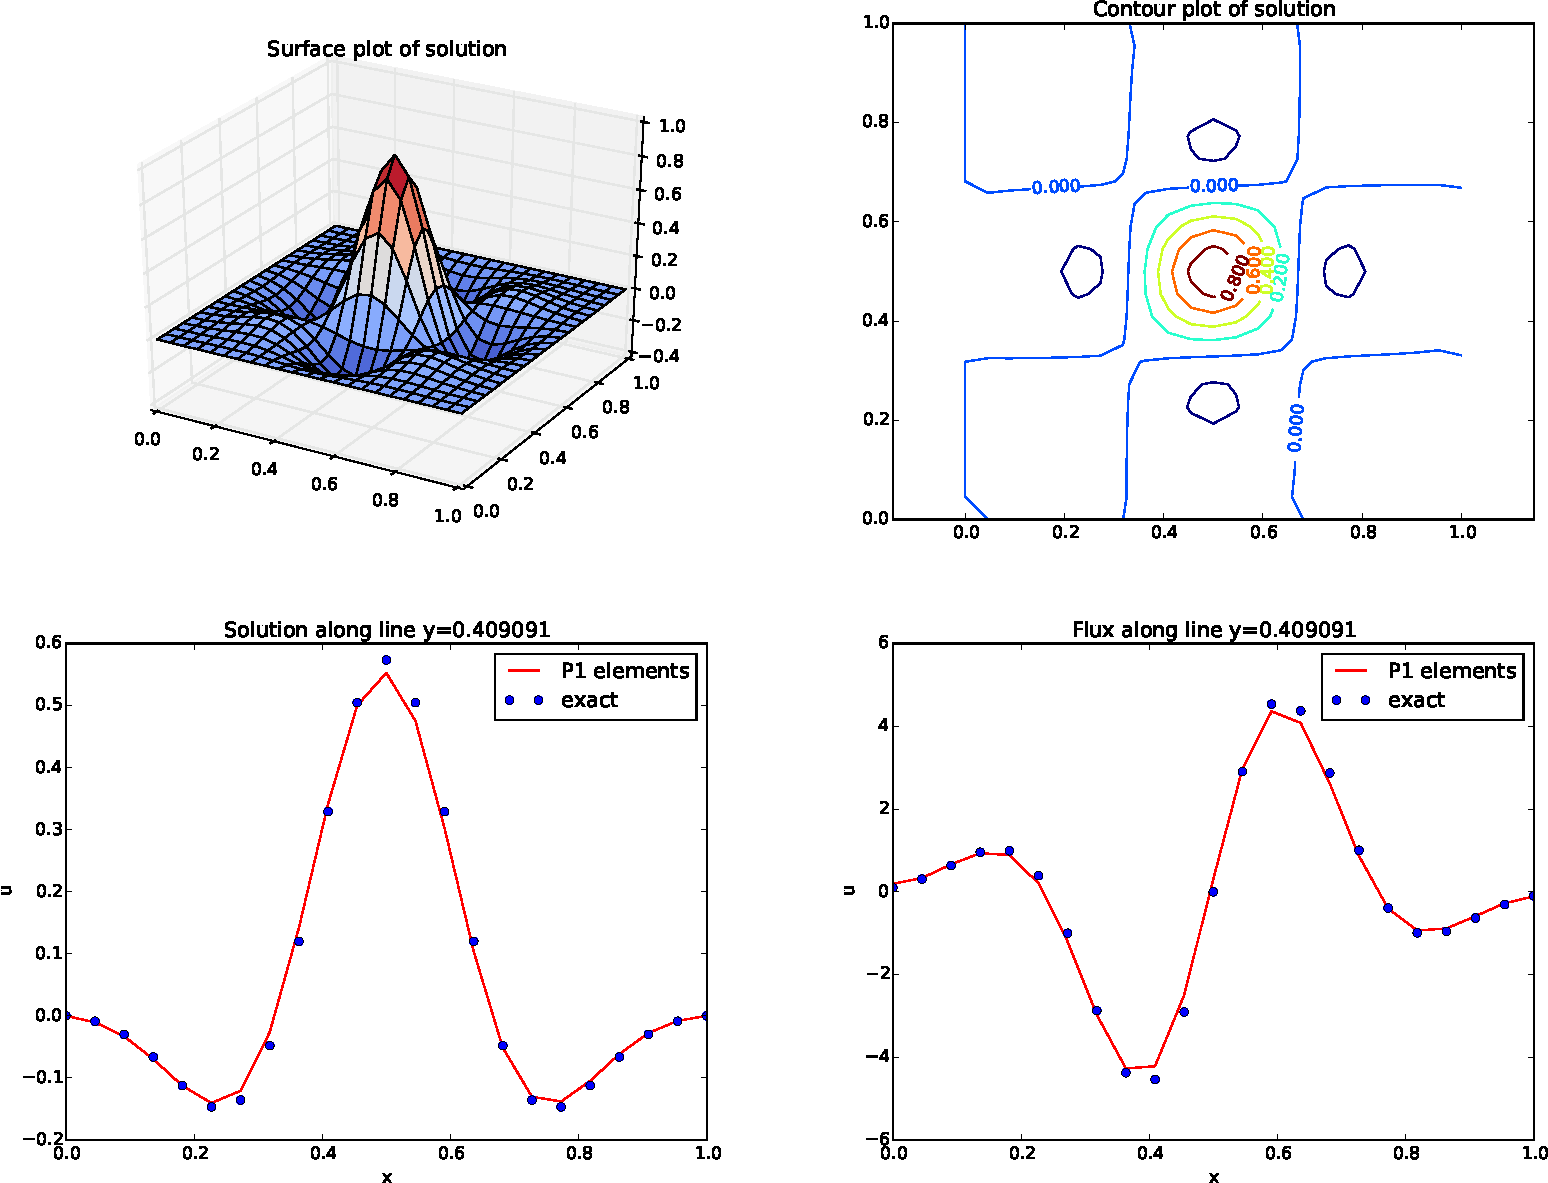
\includegraphics[width=0.95\linewidth]{fig/poisson_extended.pdf}}
  \caption{
  Various plots of the solution on a structured mesh. \label{ftut:structviz:fig1}
  }
\end{figure}
%\clearpage % flush figures ftut:structviz:fig1


\index{contour plot}

\paragraph{Making contour plots.}
A contour plot can also be made by Matplotlib:

\begin{lstlisting}[language=Python,style=graycolor]
fig = plt.figure()
ax = fig.gca()
levels = [1.5, 2.0, 2.5, 3.5]
cs = ax.contour(cv[X], cv[Y], u_, levels=levels)
plt.clabel(cs)  # add labels to contour lines
plt.axis('equal')
plt.title('Contour plot of solution')
\end{lstlisting}
The result appears in Figure~\ref{ftut:structviz:fig1} (upper right).


\paragraph{Making curve plots through the domain.}
A handy feature of \texttt{BoxField} objects is the ability to give a starting
point in the domain and a direction, and then extract the field and
corresponding coordinates along the nearest line of \emph{mesh points}. We have
already seen how to interpolate the solution along a line in the mesh, but
with \texttt{BoxField} you can pick out the computational points (vertices) for
examination of these points. Numerical methods often show improved behavior
at such points so this is of interest. For 3D fields
one can also extract data in a plane.

Say we want to plot $u$ along
the line $y=0.4$. The mesh points, \texttt{x}, and the $u$ values
along this line, \Verb!u_val!, can be extracted by

\begin{lstlisting}[language=Python,style=graycolor]
start = (0, 0.4)
x, u_val, y_fixed, snapped = u_box.gridline(start, direction=X)
\end{lstlisting}
The variable \texttt{snapped} is true if the line is snapped onto to nearest
gridline and in that case \Verb!y_fixed! holds the snapped
(altered) $y$ value. The keyword argument \texttt{snap} is by default \texttt{True}
to avoid interpolation and force snapping.

A comparison of the numerical and exact solution along the line
$y\approx 0.41$ (snapped from $y=0.4$) is made by the following code:

\begin{lstlisting}[language=Python,style=graycolor]
    # Plot u along a line y = const and compare with exact solution
    start = (0, 0.4)
    x, u_val, y_fixed, snapped = u_box.gridline(start, direction=X)
    u_e_val = [u_D((x_, y_fixed)) for x_ in x]
    plt.figure()
    plt.plot(x, u_val, 'r-')
    plt.plot(x, u_e_val, 'bo')
    plt.legend(['P1 elements', 'exact'], loc='best')
    plt.title('Solution along line y=%g' % y_fixed)
    plt.xlabel('x');  plt.ylabel('u')
\end{lstlisting}
See Figure~\ref{ftut:structviz:fig1} (lower left) for the resulting curve plot.

\paragraph{Making curve plots of the flux.}
Let us also compare the numerical and
exact fluxes $-\kappa\partial u/\partial x$ along the same line as above:

\begin{lstlisting}[language=Python,style=graycolor]
    # Plot the numerical and exact flux along the same line
    flux_u = flux(u, kappa)
    flux_u_x, flux_u_y = flux_u.split(deepcopy=True)
    flux2_x = flux_u_x if flux_u_x.ufl_element().degree() == 1 \
              else interpolate(flux_x,
                   FunctionSpace(u.function_space().mesh(), 'P', 1))
    flux_u_x_box = FEniCSBoxField(flux_u_x, (nx,ny))
    x, flux_u_val, y_fixed, snapped = \
       flux_u_x_box.gridline(start, direction=X)
    y = y_fixed
    plt.figure()
    plt.plot(x, flux_u_val, 'r-')
    plt.plot(x, flux_u_x_exact(x, y_fixed), 'bo')
    plt.legend(['P1 elements', 'exact'], loc='best')
    plt.title('Flux along line y=%g' % y_fixed)
    plt.xlabel('x');  plt.ylabel('u')
\end{lstlisting}

The function \texttt{flux} called at the beginning of the code snippet is
defined in the example program
\href{{https://fenicsproject.org/pub/tutorial/python/vol1/ft10_poisson_extended.py}}{\nolinkurl{ft10_poisson_extended.py}}
and interpolates the flux back into the function space.

Note that Matplotlib is one choice of plotting package. With the
unified interface in the \href{{https://github.com/hplgit/scitools}}{SciTools package}\footnote{\texttt{https://github.com/hplgit/scitools}} one can access Matplotlib,
Gnuplot, MATLAB, OpenDX, VisIt, and other plotting engines through the
same API.

\index{sympy@{\rm\texttt{sympy}}}

\paragraph{Test problem.}
The graphics referred to in Figure~\ref{ftut:structviz:fig1} correspond to
a test problem with prescribed solution $\uex = H(x)H(y)$, where

\[ H(x) = e^{-16(x-\frac{1}{2})^2}\sin(3\pi x)\tp\]
The corresponding right-hand side $f$ is obtained by inserting the exact
solution into the PDE and differentiating as before.
Although it is easy to carry out the
differentiation of $f$ by hand and hardcode the resulting expressions
in an \texttt{Expression} object, a more reliable habit is to use Python's
symbolic computing engine, SymPy, to perform mathematics and
automatically turn formulas into C++ syntax for \texttt{Expression} objects.
A short introduction was given in
Section~\ref{ftut:nonlinear:Newton:auto}.

We start out with defining the exact solution in \texttt{sympy}:

\begin{lstlisting}[language=Python,style=graycolor]
from sympy import exp, sin, pi  # for use in math formulas
import sympy as sym

H = lambda x: exp(-16*(x-0.5)**2)*sin(3*pi*x)
x, y = sym.symbols('x[0], x[1]')
u = H(x)*H(y)
\end{lstlisting}
Turning the expression for \texttt{u} into C or C++ syntax for \texttt{Expression} objects
needs two steps. First we ask for the C code of the expression:

\begin{lstlisting}[language=Python,style=graycolor]
u_code = sym.printing.ccode(u)
\end{lstlisting}
Printing \Verb!u_code! gives (the output is here manually broken into two
lines):

\begin{lstlisting}[language=Python,style=graycolor]
-exp(-16*pow(x[0] - 0.5, 2) - 16*pow(x[1] - 0.5, 2))*
sin(3*M_PI*x[0])*sin(3*M_PI*x[1])
\end{lstlisting}
The necessary syntax adjustment is replacing
the symbol \Verb!M_PI! for $\pi$ in C/C++ by \texttt{pi} (or \Verb!DOLFIN_PI!):

\begin{lstlisting}[language=Python,style=graycolor]
u_code = u_code.replace('M_PI', 'pi')
u_b = Expression(u_code, degree=1)
\end{lstlisting}
Thereafter, we can progress with the computation of
$f = -\nabla\cdot(\kappa\nabla u)$:

\begin{lstlisting}[language=Python,style=graycolor]
kappa = 1
f = sym.diff(-kappa*sym.diff(u, x), x) + \
    sym.diff(-kappa*sym.diff(u, y), y)
f = sym.simplify(f)
f_code = sym.printing.ccode(f)
f_code = f_code.replace('M_PI', 'pi')
f = Expression(f_code, degree=1)
\end{lstlisting}
We also need a Python function for the exact flux
$-\kappa\partial u/\partial x$:

\begin{lstlisting}[language=Python,style=graycolor]
flux_u_x_exact = sym.lambdify([x, y], -kappa*sym.diff(u, x),
                              modules='numpy')
\end{lstlisting}
It remains to define \texttt{kappa = Constant(1)} and set \texttt{nx} and \texttt{ny} before calling
\texttt{solver} to compute the finite element solution of this problem.

% FIGURE: [fig/poisson_vc_structmesh, width=800 frac=1] Various plots of the solution on a structured mesh. \label{ftut:structviz:fig1a}


% !split
\section{Taking the next step}

If you have come this far, you have learned how to both write simple
script-like solvers for a range of PDEs, and how to structure Python
solvers using functions and unit tests. Solving a more complex PDE
and writing a more full-featured PDE solver is not much harder and the
first step is typically to write a solver for a stripped-down test
case as a simple Python script. As the script matures and becomes more
complex, it is time to think about design, in particular how to
modularize the code and organize it into reusable pieces that can be
used to build a flexible and extensible solver.

On the FEniCS web site you will find more extensive documentation,
more example programs, and links to advanced solvers and applications
written on top of FEniCS. Get inspired and develop your own solver
for your favorite application, publish your code and share your
knowledge with the FEniCS community and the world!

PS: \emph{Stay tuned for the FEniCS Tutorial Volume 2!}

% !split

\clearemptydoublepage
\markboth{Bibliography}{Bibliography}
\thispagestyle{empty}

\bibliographystyle{plain}
\bibliography{bib/papers}


% ------------------- end of main content ---------------

\backmatter

% #ifdef PREAMBLE
\cleardoublepage\phantomsection  % trick to get correct link to Index
\printindex

\end{document}
% #endif
